% Copyright 2019 by Till Tantau
%
% This file may be distributed and/or modified
%
% 1. under the LaTeX Project Public License and/or
% 2. under the GNU Free Documentation License.
%
% See the file doc/generic/pgf/licenses/LICENSE for more details.


\begin{document}

% The titlepage

\pgfmathsetseed{1}
\newbox\mybox
{
  \parindent0pt
  \null
  \colorlet{mintgreen}{green!50!black!50}

  \thispagestyle{empty}
  \vskip3cm
  \vfill
  \hfil
  \begin{tikzpicture}[overlay]
    \coordinate (front) at (0,0);
    \coordinate (horizon) at (0,.31\paperheight);
    \coordinate (bottom) at (0,-.6\paperheight);
    \coordinate (sky) at (0,.57\paperheight);
    \coordinate (left) at (-.51\paperwidth,0);
    \coordinate (right) at (.51\paperwidth,0);

    \shade [bottom color=blue!30!black!10,top color=blue!30!black!50]
      ([yshift=-5mm]horizon -|  left) rectangle (sky -| right);
    \shade [bottom color=black!70!green!25,top color=black!70!green!10]
      (front -| left) -- (horizon -| left)
      decorate [decoration=random steps] { -- (horizon -| right) }
      -- (front -| right) -- cycle;
    \shade [top color=black!70!green!25,bottom color=black!25]
      ([yshift=-5mm-1pt]front -| left) rectangle ([yshift=1pt]front -| right);
    \fill [black!25] (bottom -| left) rectangle ([yshift=-5mm]front -| right);

    \def\nodeshadowed[#1]#2;{\node[scale=2,above,#1]{\global\setbox\mybox=\hbox{#2}\copy\mybox};
      \node[scale=2,above,#1,yscale=-1,scope fading=south,opacity=0.4]{\box\mybox};}

    \nodeshadowed [at={(-5,5  )},yslant=0.05] {\Huge Ti\textcolor{orange}{\emph{k}}Z};
    \nodeshadowed [at={( 0,5.3)}] {\huge \textcolor{mintgreen}{\&}};
    \nodeshadowed [at={( 5,5  )},yslant=-0.05] {\Huge \textsc{PGF}};
    \nodeshadowed [at={( 0,2  )}] {Manual for Version \pgftypesetversion};

    \foreach \where in {-9cm,9cm}
    {\nodeshadowed [at={(\where,5cm)}] {
    % TODO: Nesting tikzpictures is NOT supported
    \tikz \draw [green!20!black, rotate=90]
    [l-system={rule set={F -> FF-[-F+F]+[+F-F]}, axiom=F, order=4,
      step=2pt, randomize step percent=50, angle=30, randomize angle percent=5}]
    lindenmayer system;};}

    \foreach \i in {0.5,0.6,...,2}
      \fill [white,decoration=Koch snowflake,opacity=.9]
            [shift=(horizon),shift={(rand*11,rnd*7)},scale=\i]
            [double copy shadow={opacity=0.2,shadow xshift=0pt,shadow
              yshift=3*\i pt,fill=white,draw=none}]
        decorate {
          decorate {
            decorate {
              (0,0) -- ++(60:1) -- ++(-60:1) -- cycle
            }
          }
        };

  \node (left text) [text width=.5\paperwidth-2cm,below right,at={(-.5\paperwidth+1cm,-1.5cm)}]
  {
    \fontencoding{T1}
    \fontfamily{pcr}
    \def\textbraceleft{\char`\{}
    \def\textbraceright{\char`\}}
    \def\textbackslash{\char`\\}
    \begin{lstlisting}[basicstyle=\scriptsize\color{black},
                       keywordstyle=\bfseries\color{white},
                       identifierstyle=\bfseries\color{black},
                       keywords={tikzpicture,shade,fill,draw,path,node},
                       literate={-}{{-}}1]
\begin{tikzpicture}
  \coordinate (front) at (0,0);
  \coordinate (horizon) at (0,.31\paperheight);
  \coordinate (bottom) at (0,-.6\paperheight);
  \coordinate (sky) at (0,.57\paperheight);
  \coordinate (left) at (-.51\paperwidth,0);
  \coordinate (right) at (.51\paperwidth,0);

  \shade [bottom color=white,
          top color=blue!30!black!50]
              ([yshift=-5mm]horizon -|  left)
    rectangle (sky -| right);

  \shade [bottom color=black!70!green!25,
          top color=black!70!green!10]
    (front -| left) -- (horizon -| left)
    decorate [decoration=random steps] {
      -- (horizon -| right)  }
    -- (front -| right) -- cycle;

  \shade [top color=black!70!green!25,
         bottom color=black!25]
              ([yshift=-5mm-1pt]front -| left)
    rectangle ([yshift=1pt]front -| right);

  \fill [black!25]
              (bottom -| left)
    rectangle ([yshift=-5mm]front -| right);

  \def\nodeshadowed[#1]#2;{
    \node[scale=2,above,#1]{
      \global\setbox\mybox=\hbox{#2}
      \copy\mybox};
    \node[scale=2,above,#1,yscale=-1,
          scope fading=south,opacity=0.4]{\box\mybox};
  }
\end{lstlisting}
};

  \node (right text) [text width=.5\paperwidth-2cm,below right,at={(1cm,-1.5cm)}]
  {
    \fontencoding{T1}
    \fontfamily{pcr}
    \def\textbraceleft{\char`\{}
    \def\textbraceright{\char`\}}
    \def\textbackslash{\char`\\}
    \begin{lstlisting}[basicstyle=\scriptsize\color{black},
                       keywordstyle=\bfseries\color{white},
                       identifierstyle=\bfseries\color{black},
                       keywords={tikzpicture,shade,fill,draw,path,node},
                       literate={-}{{-}}1]
  \nodeshadowed [at={(-5,8  )},yslant=0.05]
    {\Huge Ti\textcolor{orange}{\emph{k}}Z};
  \nodeshadowed [at={( 0,8.3)}]
    {\huge \textcolor{green!50!black!50}{\&}};
  \nodeshadowed [at={( 5,8  )},yslant=-0.05]
    {\Huge \textsc{PGF}};
  \nodeshadowed [at={( 0,5  )}]
    {Manual for Version \pgftypesetversion};

  \foreach \where in {-9cm,9cm} {
    \nodeshadowed [at={(\where,5cm)}] { \tikz
      \draw [green!20!black, rotate=90,
             l-system={rule set={F -> FF-[-F+F]+[+F-F]},
               axiom=F, order=4,step=2pt,
               randomize step percent=50, angle=30,
               randomize angle percent=5}] l-system; }}

  \foreach \i in {0.5,0.6,...,2}
    \fill
      [white,opacity=\i/2,
       decoration=Koch snowflake,
       shift=(horizon),shift={(rand*11,rnd*7)},
       scale=\i,double copy shadow={
         opacity=0.2,shadow xshift=0pt,
         shadow yshift=3*\i pt,fill=white,draw=none}]
      decorate {
        decorate {
          decorate {
            (0,0)- ++(60:1) -- ++(-60:1) -- cycle
          } } };

   \node (left text) ...
   \node (right text) ...

   \fill [decorate,decoration={footprints,foot of=gnome},
          opacity=.5,brown]        (rand*8,-rnd*10)
     to [out=rand*180,in=rand*180] (rand*8,-rnd*10);
\end{tikzpicture}
  \end{lstlisting}
  };

  \fill [decorate,decoration=footprints,
         decoration={footprints,foot of=gnome},
         opacity=.5,brown]        (rand*8,-rnd*10)
    to [out=rand*180,in=rand*180] (rand*8,-rnd*10);
\end{tikzpicture}
\vfill
\vbox{}
\clearpage
}

{
  \vbox{}
  \vskip0pt plus 1fill
  Für meinen Vater, damit er noch viele schöne \TeX-Graphiken
  erschaffen kann.
  \vskip1em
  \hfill\emph{Till}
  \vskip0pt plus 3fill

  \parindent=0pt
  Copyright 2007 to 2013 by Till Tantau

  \medskip
  Permission is granted to copy, distribute and/or modify \emph{the
  documentation} under the terms of the \textsc{gnu} Free Documentation
  License, Version 1.2 or any later version published by the Free Software
  Foundation; with no Invariant Sections, no Front-Cover Texts, and no
  Back-Cover Texts. A copy of the license is included in the section entitled
  \textsc{gnu} Free Documentation License.

  \medskip
  Permission is granted to copy, distribute and/or modify \emph{the code of the
  package} under the terms of the \textsc{gnu} Public License, Version 2 or any
  later version published by the Free Software Foundation. A copy of the
  license is included in the section entitled \textsc{gnu} Public License.

  \medskip
  Permission is also granted to distribute and/or modify \emph{both the
  documentation and the code} under the conditions of the LaTeX Project Public
  License, either version 1.3 of this license or (at your option) any later
  version. A copy of the license is included in the section entitled \LaTeX\
  Project Public License.

  \vbox{}
  \clearpage
}


\title{\bfseries \tikzname\ 和 {\Large PGF} 宏包\\
  \large 版本 \pgfversion{} 的文档\\[1mm]
\large\href{https://github.com/pgf-tikz/pgf}{\texttt{https://github.com/pgf-tikz/pgf}}}
\author{Till Tantau\footnote{Editor of this documentation. Parts of
    this documentation have been written by other authors as indicated
    in these parts or chapters and in Section~\ref{section-authors}.}\\
  \normalsize Institut für Theoretische Informatik\\[-1mm]
  \normalsize Universität zu Lübeck}

\maketitle
\label{table-of-contents}

\tableofcontents

\clearpage


% Copyright 2019 by Till Tantau
%
% This file may be distributed and/or modified
%
% 1. under the LaTeX Project Public License and/or
% 2. under the GNU Free Documentation License.
%
% See the file doc/generic/pgf/licenses/LICENSE for more details.


\section{介绍}

欢迎来到 \tikzname\ 和底层 \pgfname\ 系统的文档。
What began as a small \LaTeX\ style for creating the graphics in my (Till
Tantau's) PhD thesis directly with pdf\LaTeX\ has now grown to become a
full-blown graphics language with a manual of over a thousand pages. The wealth
of options offered by \tikzname\ is often daunting to beginners; but
fortunately this documentation comes with a number of slowly-paced tutorials that
will teach you almost all you should know about \tikzname\ without your having
to read the rest.

I wish to start with the question ``What is \tikzname?'' Basically, it just
defines a number of \TeX\ commands that draw graphics. For example, the code
|\tikz \draw (0pt,0pt) -- (20pt,6pt);| yields the line \tikz \draw (0pt,0pt) --
(20pt,6pt); and the code |\tikz \fill[orange] (1ex,1ex) circle (1ex);| yields
\tikz \fill[orange] (1ex,1ex) circle (1ex);. In a sense, when you use
\tikzname\ you ``program'' your graphics, just as you ``program'' your document
when you use \TeX. This also explains the name: \tikzname\ is a recursive
acronym in the tradition of ``\textsc{gnu}'s Not Unix'' and means ``\tikzname\
ist \emph{kein} Zeichenprogramm'', which translates to ``\tikzname\ is not a
drawing program'', cautioning the reader as to what to expect. With \tikzname\
you get all the advantages of the ``\TeX-approach to typesetting'' for your
graphics: quick creation of simple graphics, precise positioning, the use of
macros, often superior typography. You also inherit all the disadvantages:
steep learning curve, no \textsc{wysiwyg}, small changes require a long
recompilation time, and the code does not really ``show'' how things will look
like.

Now that we know what \tikzname\ is, what about ``\pgfname''? As mentioned
earlier, \tikzname\ started out as a project to implement \TeX\ graphics macros
that can be used both with pdf\LaTeX\ and also with the classical
(PostScript-based) \LaTeX. In other words, I wanted to implement a ``portable
graphics format'' for \TeX\ -- hence the name \pgfname. These early macros are
still around and they form the ``basic layer'' of the system described in this
manual, but most of the interaction an author has these days is with
\tikzname\ -- which has become a whole language of its own.


\subsection{The Layers Below \tikzname}

It turns out that there are actually \emph{two} layers below \tikzname:
%
\begin{description}
    \item[System layer:] This layer provides a complete abstraction of what
        is going on ``in the driver''. The driver is a program like |dvips|
        or |dvipdfm| that takes a |.dvi| file as input and generates a |.ps|
        or a |.pdf| file. (The |pdftex| program also counts as a driver, even
        though it does not take a |.dvi| file as input. Never mind.) Each
        driver has its own syntax for the generation of graphics, causing
        headaches to everyone who wants to create graphics in a portable way.
        \pgfname's system layer ``abstracts away'' these differences. For
        example, the system command |\pgfsys@lineto{10pt}{10pt}| extends the
        current path  to the coordinate $(10\mathrm{pt},10\mathrm{pt})$ of
        the current |{pgfpicture}|. Depending on whether |dvips|, |dvipdfm|,
        or |pdftex| is used to process the document, the system command will
        be converted to different |\special| commands. The system layer is as
        ``minimalistic'' as possible since each additional command makes it
        more work to port \pgfname\ to a new driver.

        As a user, you will not use the system layer directly.
    \item[Basic layer:] The basic layer provides a set of basic commands that
        allow you to produce complex graphics in a much easier manner than by
        using the system layer directly. For example, the system layer provides
        no commands for creating circles since circles can be composed from the
        more basic Bézier curves (well, almost). However, as a user you will
        want to have a simple command to create circles (at least I do) instead
        of having to write down half a page of Bézier curve support
        coordinates. Thus, the basic layer provides a command |\pgfpathcircle|
        that generates the necessary curve coordinates for you.

        The basic layer consists of a \emph{core}, which consists of several
        interdependent packages that can only be loaded \emph{en bloc}, and
        additional \emph{modules} that extend the core by more
        special-purpose commands like node management or a plotting
        interface. For instance, the \textsc{beamer} package uses only the
        core and not, say, the |shapes| modules.
\end{description}

In theory, \tikzname\ itself is just one of several possible ``frontends''.
which are sets of commands or a special syntax that makes using the basic layer
easier. A problem with directly using the basic layer is that code written for
this layer is often too ``verbose''. For example, to draw a simple triangle,
you may need as many as five commands when using the basic layer: One for
beginning a path at the first corner of the triangle, one for extending the
path to the second corner, one for going to the third, one for closing the
path, and one for actually painting the triangle (as opposed to filling it).
With the \tikzname\ frontend all this boils down to a single simple
\textsc{metafont}-like command:
%
\begin{verbatim}
\draw (0,0) -- (1,0) -- (1,1) -- cycle;
\end{verbatim}

In practice, \tikzname\ is the only ``serious'' frontend for \pgfname. It gives
you access to all features of \pgfname, but it is intended to be easy to use.
The syntax is a mixture of \textsc{metafont} and \textsc{pstricks} and some
ideas of myself. There are other frontends besides \tikzname, but they are intended
more as ``technology studies'' and less as serious alternatives to
\tikzname. In particular, the |pgfpict2e| frontend   reimplements the standard
\LaTeX\ |{picture}|  environment and commands like |\line| or |\vector| using
the \pgfname\ basic layer. This layer is not really ``necessary'' since the
|pict2e.sty| package does at least as good a job at reimplementing the
|{picture}| environment. Rather, the idea behind this package is to have a
simple demonstration of how a frontend can be implemented.

Since most users will only use \tikzname\ and almost no one will use the system
layer directly, this manual is mainly about \tikzname\ in the first parts; the
basic layer and the system layer are explained at the end.


\subsection{Comparison with Other Graphics Packages}

\tikzname\ is not the only graphics package for \TeX. In the following, I try
to give a reasonably fair comparison of \tikzname\ and other packages.
%
\begin{enumerate}
    \item The standard \LaTeX\ |{picture}| environment allows you to create
        simple graphics, but little more. This is certainly not due to a lack
        of knowledge or imagination on the part of \LaTeX's designer(s).
        Rather, this is the price paid for the |{picture}| environment's
        portability: It works together with all backend drivers.
    \item The |pstricks| package is certainly powerful enough to create any
        conceivable kind of graphic, but it is not really portable. Most
        importantly, it does not work with |pdftex| nor with any other driver
        that produces anything but PostScript code.

        Compared to \tikzname, |pstricks| has a similar support base. There
        are many nice extra packages for special purpose situations that have
        been contributed by users over the last decade. The \tikzname\ syntax
        is more consistent than the |pstricks| syntax as \tikzname\ was
        developed ``in a more centralized manner'' and also ``with the
        shortcomings on |pstricks| in mind''.
    \item The |xypic| package is an older package for creating graphics.
        However, it is more difficult to use and to learn because the syntax
        and the documentation are a bit cryptic.
    \item The |dratex| package is a small graphic package for creating a
        graphics. Compared to the other package, including \tikzname, it is
        very small, which may or may not be an advantage.
    \item The |metapost| program is a powerful alternative to \tikzname. It
        used to be an external program, which entailed a bunch of problems,
        but in Lua\TeX\ it is now built in. An obstacle with |metapost| is
        the inclusion of labels. This is \emph{much} easier to achieve using
        \pgfname.
    \item The |xfig| program is an important alternative to \tikzname\ for
        users who do not wish to ``program'' their graphics as is necessary
        with \tikzname\ and the other packages above. There is a conversion
        program that will convert |xfig| graphics to \tikzname.
\end{enumerate}


\subsection{Utility Packages}

The \pgfname\ package comes along with a number of utility package that are not
really about creating graphics and which can be used independently of \pgfname.
However, they are bundled with \pgfname, partly out of convenience, partly
because their functionality is closely intertwined with \pgfname. These utility
packages are:
%
\begin{enumerate}
    \item The |pgfkeys| package defines a powerful key management facility.
        It can be used completely independently of \pgfname.
    \item The |pgffor| package defines a useful |\foreach| statement.
    \item The |pgfcalendar| package defines macros for creating calendars.
        Typically, these calendars will be rendered using \pgfname's graphic
        engine, but you can use |pgfcalendar| also typeset calendars using
        normal text. The package also defines commands for ``working'' with
        dates.
    \item The |pgfpages| package is used to assemble several pages into a
        single page. It provides commands for assembling several ``virtual
        pages'' into a single ``physical page''. The idea is that whenever
        \TeX\ has a page ready for ``shipout'', |pgfpages| interrupts this
        shipout and instead stores the page to be shipped out in a special
        box. When enough ``virtual pages'' have been accumulated in this way,
        they are scaled down and arranged on a ``physical page'', which then
        \emph{really} shipped out. This mechanism allows you to create ``two
        page on one page'' versions of a document directly inside \LaTeX\
        without the use of any external programs. However, |pgfpages| can do
        quite a lot more than that. You can use it to put logos and watermark
        on pages, print up to 16 pages on one page, add borders to pages, and
        more.
\end{enumerate}


\subsection{How to Read This Manual}

This manual describes both the design of \tikzname\ and its usage. The
organization is very roughly according to ``user-friendliness''. The commands
and subpackages that are easiest and most frequently used are described first,
more low-level and esoteric features are discussed later.

If you have not yet installed \tikzname, please read the installation first.
Second, it might be a good idea to read the tutorial. Finally, you might wish
to skim through the description of \tikzname. Typically, you will not need to
read the sections on the basic layer. You will only need to read the part on
the system layer if you intend to write your own frontend or if you wish to
port \pgfname\ to a new driver.

The ``public'' commands and environments provided by the system are described
throughout the text. In each such description, the described command,
environment or option is printed in red. Text shown in green is optional and
can be left out.


\subsection{Authors and Acknowledgements}
\label{section-authors}

The bulk of the \pgfname\ system and its documentation was written by Till
Tantau. A further member of the main team is Mark Wibrow, who is responsible,
for example, for the \pgfname\ mathematical engine, many shapes, the decoration
engine, and matrices. The third member is Christian Feuers\"anger who
contributed the floating point library, image externalization, extended key
processing, and automatic hyperlinks in the manual.

Furthermore, occasional contributions have been made by Christophe Jorssen,
Jin-Hwan Cho, Olivier Binda, Matthias Schulz, Ren\'ee Ahrens, Stephan Schuster,
and Thomas Neumann.

Additionally, numerous people have contributed to the \pgfname\ system by
writing emails, spotting bugs, or sending libraries and patches. Many thanks to
all these people, who are too numerous to name them all!


\subsection{Getting Help}

When you need help with \pgfname\ and \tikzname, please do the following:

\begin{enumerate}
    \item Read the manual, at least the part that has to do with your
        problem.
    \item If that does not solve the problem, try having a look at the
        GitHub development page for \pgfname\ and \tikzname\ (see the
        title of this document). Perhaps someone has already reported a
        similar problem and someone has found a solution.
    \item On the website you will find numerous forums for getting help.
        There, you can write to help forums, file bug reports, join mailing
        lists, and so on.
    \item Before you file a bug report, especially a bug report concerning
        the installation, make sure that this is really a bug. In particular,
        have a look at the |.log| file that results when you \TeX\ your
        files. This |.log| file should show that all the right files are
        loaded from the right directories. Nearly all installation problems
        can be resolved by looking at the |.log| file.
    \item \emph{As a last resort} you can try to email me (Till Tantau) or,
        if the problem concerns the mathematical engine, Mark Wibrow. I do
        not mind getting emails, I simply get way too many of them. Because
        of this, I cannot guarantee that your emails will be answered in a 
        timely fashion or even at all. Your chances that your problem will
        be fixed are somewhat higher if you mail to the \pgfname\ mailing
        list (naturally, I read this list and answer questions when I have
        the time).
\end{enumerate}


\end{document} % for quick test


\part{Tutorials and Guidelines}

{\Large \emph{by Till Tantau}}

\bigskip
\noindent To help you get started with \tikzname, instead of a long
installation and configuration section, this manual starts with tutorials. They
explain all the basic and some of the more advanced features of the system,
without going into all the details. This part also contains some guidelines on
how you should proceed when creating graphics using \tikzname.

\vskip3cm

\begin{codeexample}[graphic=white,width=0pt]
\tikz \draw[thick,rounded corners=8pt]
  (0,0) -- (0,2) -- (1,3.25) -- (2,2) -- (2,0) -- (0,2) -- (2,2) -- (0,0) -- (2,0);
\end{codeexample}


\include{pgfmanual-en-tutorial}
\include{pgfmanual-en-tutorial-nodes}
\include{pgfmanual-en-tutorial-Euclid}
\include{pgfmanual-en-tutorial-chains}
\include{pgfmanual-en-tutorial-map}
\include{pgfmanual-en-guidelines}



\part{Installation and Configuration}

{\Large \emph{by Till Tantau}}


\bigskip
\noindent This part explains how the system is installed. Typically, someone
has already done so for your system, so this part can be skipped; but if this
is not the case and you are the poor fellow who has to do the installation,
read the present part.


\vskip1cm

\begin{codeexample}[graphic=white,preamble={\usetikzlibrary{arrows.meta,automata,positioning,shadows}}]
\begin{tikzpicture}[->,>={Stealth[round]},shorten >=1pt,auto,node distance=2.8cm,on grid,semithick,
                    every state/.style={fill=red,draw=none,circular drop shadow,text=white}]

  \node[initial,state] (A)                    {$q_a$};
  \node[state]         (B) [above right=of A] {$q_b$};
  \node[state]         (D) [below right=of A] {$q_d$};
  \node[state]         (C) [below right=of B] {$q_c$};
  \node[state]         (E) [below=of D]       {$q_e$};

  \path (A) edge              node {0,1,L} (B)
            edge              node {1,1,R} (C)
        (B) edge [loop above] node {1,1,L} (B)
            edge              node {0,1,L} (C)
        (C) edge              node {0,1,L} (D)
            edge [bend left]  node {1,0,R} (E)
        (D) edge [loop below] node {1,1,R} (D)
            edge              node {0,1,R} (A)
        (E) edge [bend left]  node {1,0,R} (A);

   \node [right=1cm,text width=8cm] at (C)
   {
     The current candidate for the busy beaver for five states. It is
     presumed that this Turing machine writes a maximum number of
     $1$'s before halting among all Turing machines with five states
     and the tape alphabet $\{0, 1\}$. Proving this conjecture is an
     open research problem.
   };
\end{tikzpicture}
\end{codeexample}


\include{pgfmanual-en-installation}
\include{pgfmanual-en-license}
\include{pgfmanual-en-drivers}



\part{Ti\emph{k}Z ist \emph{kein} Zeichenprogramm}
\label{part-tikz}

{\Large \emph{by Till Tantau}}


\bigskip
\noindent
\vskip3cm
\begin{codeexample}[graphic=white,preamble={\usetikzlibrary{angles,calc,quotes}}]
\begin{tikzpicture}[angle radius=.75cm]

  \node (A) at (-2,0)     [red,left]   {$A$};
  \node (B) at ( 3,.5)    [red,right]  {$B$};
  \node (C) at (-2,2)     [blue,left]  {$C$};
  \node (D) at ( 3,2.5)   [blue,right] {$D$};
  \node (E) at (60:-5mm)  [below]      {$E$};
  \node (F) at (60:3.5cm) [above]      {$F$};

  \coordinate (X) at (intersection cs:first line={(A)--(B)}, second line={(E)--(F)});
  \coordinate (Y) at (intersection cs:first line={(C)--(D)}, second line={(E)--(F)});

  \path
    (A) edge [red, thick]  (B)
    (C) edge [blue, thick] (D)
    (E) edge [thick]       (F)
      pic ["$\alpha$", draw, fill=yellow]   {angle = F--X--A}
      pic ["$\beta$",  draw, fill=green!30] {angle = B--X--F}
      pic ["$\gamma$", draw, fill=yellow]   {angle = E--Y--D}
      pic ["$\delta$", draw, fill=green!30] {angle = C--Y--E};

  \node at ($ (D)!.5!(B) $) [right=1cm,text width=6cm,rounded corners,fill=red!20,inner sep=1ex]
    {
      When we assume that $\color{red}AB$ and $\color{blue}CD$ are
      parallel, i.\,e., ${\color{red}AB} \mathbin{\|} \color{blue}CD$,
      then $\alpha = \gamma$ and $\beta = \delta$.
    };
\end{tikzpicture}
\end{codeexample}


\include{pgfmanual-en-tikz-design}
\include{pgfmanual-en-tikz-scopes}
\include{pgfmanual-en-tikz-coordinates}
\include{pgfmanual-en-tikz-paths}
\include{pgfmanual-en-tikz-actions}
\include{pgfmanual-en-tikz-arrows}
% Copyright 2019 by Till Tantau
%
% This file may be distributed and/or modified
%
% 1. under the LaTeX Project Public License and/or
% 2. under the GNU Free Documentation License.
%
% See the file doc/generic/pgf/licenses/LICENSE for more details.


\section{Nodes and Edges}
\label{section-nodes}

\subsection{Overview}

In the present section, the usage of \emph{nodes} in \tikzname\ is explained. A
node is typically a rectangle or circle or another simple shape with some text
on it.

Nodes are added to paths using the special path operation |node|. Nodes
\emph{are not part of the path itself}. Rather, they are added to the picture
just before or after the path has been drawn.

In Section~\ref{section-nodes-basic} the basic syntax of the node operation is
explained, followed in Section~\ref{section-nodes-multi} by the syntax for
multi-part nodes, which are nodes that contain several different text parts.
After this, the different options for the text in nodes are explained. In
Section~\ref{section-nodes-anchors} the concept of \emph{anchors} is introduced
along with their usage. In Section~\ref{section-nodes-transformations} the
different ways transformations affect nodes are studied.
Sections~\ref{section-nodes-placing-1} and~\ref{section-nodes-placing-2} are
about placing nodes on or next to straight lines and curves.
Section~\ref{section-nodes-connecting} explains how a node can be used as a
``pseudo-coordinate''. Section~\ref{section-nodes-edges} introduces the |edge|
operation, which works similar to the |to| operation and also similar to the
|node| operation.


\subsection{Nodes and Their Shapes}
\label{section-nodes-basic}

In the simplest case, a node is just some text that is placed at some
coordinate. However, a node can also have a border drawn around it or have a
more complex background and foreground. Indeed, some nodes do not have a text
at all, but consist solely of the background. You can name nodes so that you
can reference their coordinates later in the same picture or, if certain
precautions are taken as explained in Section~\ref{section-cross-picture-tikz},
also in different pictures.

There are no special \TeX\ commands for adding a node to a picture; rather,
there is path operation called |node| for this. Nodes are created whenever
\tikzname\ encounters |node| or |coordinate| at a point on a path where it
would expect a normal path operation (like |-- (1,1)| or |rectangle (1,1)|). It
is also possible to give node specifications \emph{inside} certain path
operations as explained later.

The node operation is typically followed by some options, which apply only to
the node. Then, you can optionally \emph{name} the node by providing a name in
parentheses. Lastly, for the |node| operation you must provide some label text
for the node in curly braces, while for the |coordinate| operation you may not.
The node is placed at the current position of the path either \emph{after the
path has been drawn} or (more seldomly and only if you add the |behind path|
option) \emph{just before the path is drawn.} Thus, all nodes are drawn ``on
top'' or ``behind'' the path and are retained until the path is complete. If
there are several nodes on a path, perhaps some behind and some on top of the
path, first come the nodes behind the path in the order they were encountered,
then comes that path, and then come the remaining node, again in the order they
are encountered.
%
\begin{codeexample}[]
\tikz \fill [fill=yellow!80!black]
     (0,0) node              {first node}
  -- (1,1) node[behind path] {second node}
  -- (2,0) node              {third node};
\end{codeexample}


\subsubsection{Syntax of the Node Command}

The syntax for specifying nodes is the following:
%
\begin{pathoperation}{node}{
    \opt{\meta{foreach statements}}
    \opt{|[|\meta{options}|]|}
    \opt{|(|\meta{name}|)|}
    \opt{|at(|\meta{coordinate}|)|}
    \opt{|:|\meta{animation attribute}|=|\marg{options}}
    \opt{\marg{node contents}}%
}
    Since this path operation is one of the most involved around, let us go
    over it step by step.

    \medskip
    \textbf{Order of the parts of the specification.}
    Everything between ``|node|'' and the opening brace of a node is optional.
    If there are \meta{foreach statements}, they must come first, directly
    following ``|node|''. Other than that, the ordering of all the other
    elements of a node specification (the \meta{options}, the  \meta{name},
    \meta{coordinate}, and \meta{animation attribute}) is arbitrary, indeed,
    there can be multiple occurrences of any of these elements (although for
    the name and the coordinate this makes no sense).

    \medskip
    \textbf{The text of a node.}
    At the end of a node, you must (normally) provide some \meta{node contents}
    in curly braces; indeed, the ``end'' of the node specification is detected
    by the opening curly brace. For normal nodes it is possible to use
    ``fragile'' stuff inside the \meta{node contents} like the |\verb| command
    (for the technically savvy: code inside the \meta{node contents} is allowed
    to change catcodes; however, this rule does not apply to ``nodes on a
    path'' to be discussed later).

    Instead of giving \meta{node contents} at the end of the node in curly
    braces, you can also use the following key:
    %
    \begin{key}{/tikz/node contents=\meta{node contents}}
    \label{option-node-contents}%
        This key sets the contents of the node to the given text as if you had
        given it at the end in curly braces. When the option is used inside the
        options of a node, the parsing of the node stops immediately after the
        end of the option block. In particular, the option block cannot be
        followed by further option blocks or curly braces (or, rather, these do
        not count as part of the node specification.) Also note that the
        \meta{node contents} may not contain fragile stuff since the catcodes
        get fixed upon reading the options. Here is an example:
        %
\begin{codeexample}[]
\tikz {
  \path (0,0) node [red]                    {A}
        (1,0) node [blue]                   {B}
        (2,0) node [green, node contents=C]
        (3,0) node [node contents=D]           ;
}
\end{codeexample}
        %
\end{key}

    \medskip
    \textbf{Specifying the location of the node.}
    Nodes are placed at the last position mentioned on the path. The effect of
    adding ``|at|'' to a node specification is that the coordinate given after
    |at| is used instead. The |at| syntax is not available when a node is given
    inside a path operation (it would not make any sense there).

    \begin{key}{/tikz/at=\meta{coordinate}}
        This is another way of specifying the |at| coordinate. Note that,
        typically, you will have to enclose the \meta{coordinate} in curly
        braces so that a comma inside the \meta{coordinate} does not confuse
        \TeX.
    \end{key}

    Another aspect of the ``location'' of a node is whether it appears \emph{in
    front of} or \emph{behind} the current path. You can change which of these
    two possibilities happens on a node-by-node basis using the following keys:
    %
    \begin{key}{/tikz/behind path}
        When this key is set, either as a local option for the node or some
        surrounding scope, the node will be drawn behind the current path. For
        this, \tikzname\ collects all nodes defined on the current path with
        this option set and then inserts all of them, in the order they appear,
        just before it draws the path. Thus, several nodes with this option set
        may obscure one another, but never the path itself. ``Just before it
        draws the path'' actually means that the nodes are inserted into the
        page output just before any pre-actions are applied to the path (see
        below for what pre-actions are).
        %
\begin{codeexample}[]
\tikz \fill [fill=blue!50, draw=blue, very thick]
      (0,0)   node [behind path, fill=red!50]   {first node}
   -- (1.5,0) node [behind path, fill=green!50] {second node}
   -- (1.5,1) node [behind path, fill=brown!50] {third node}
   -- (0,1)   node [             fill=blue!30]  {fourth node};
\end{codeexample}

        Note that |behind path| only applies to the current path; not to the
        current scope or picture. To put a node ``behind everything'' you need
        to use layers and options like |on background layer|, see the
        |backgrounds| library in Section~\ref{section-tikz-backgrounds}.
    \end{key}

    \begin{key}{/tikz/in front of path}
        This is the opposite of |behind path|: It causes nodes to be drawn on
        top of the path. Since this is the default behavior, you usually do
        not need this option; it is only needed when an enclosing scope has
        used |behind path| and you now wish to ``switch back'' to the normal
        behavior.
    \end{key}

    \medskip
    \textbf{The name of a node.}
    The |(|\meta{name}|)| is a name for later reference and it is optional. You
    may also add the option |name=|\meta{name} to the \meta{option} list; it
    has the same effect.

    \begin{key}{/tikz/name=\meta{node name}}
        Assigns a name to the node for later reference. Since this is a
        ``high-level'' name (drivers never know of it), you can use spaces,
        number, letters, or whatever you like when naming a node. Thus, you can
        name a node just |1| or perhaps |start of chart| or even |y_1|. Your
        node name should \emph{not} contain any punctuation like a dot, a
        comma, or a colon since these are used to detect what kind of
        coordinate you mean when you reference a node.
    \end{key}

    \begin{key}{/tikz/alias=\meta{another node name}}
        This option allows you to provide another name for the node. Giving
        this option multiple times will allow you to access the node via
        several aliases. Using the |node also| syntax, you can also assign an
        alias name to a node at a later point, see
        Section~\ref{section-node-also}.
    \end{key}

    \medskip
    \textbf{The options of a node.}
    The \meta{options} is an optional list of options that \emph{apply only to
    the node} and have no effect outside. The other way round, most ``outside''
    options also apply to the node, but not all. For example, the ``outside''
    rotation does not apply to nodes (unless some special options are used,
    sigh). Also, the outside path action, like |draw| or |fill|, never applies
    to the node and must be given in the node (unless some special other
    options are used, deep sigh).

    \medskip
    \textbf{The shape of a node.}
    As mentioned before, we can add a border and even a background to a node:
    %
\begin{codeexample}[]
\tikz \fill[fill=yellow!80!black]
      (0,0) node {first node}
   -- (1,1) node[draw, behind path] {second node}
   -- (0,2) node[fill=red!20,draw,double,rounded corners] {third node};
\end{codeexample}

    The ``border'' is actually just a special case of a much more general
    mechanism. Each node has a certain \emph{shape} which, by default, is a
    rectangle. However, we can also ask \tikzname\ to use a circle shape
    instead or an ellipse shape (you have to include one of the
    |shapes.geometric| library for the latter shape):
    %
\begin{codeexample}[preamble={\usetikzlibrary{shapes.geometric}}]
\tikz \fill[fill=yellow!80!black]
      (0,0) node                            {first node}
   -- (1,1) node[ellipse,draw, behind path] {second node}
   -- (0,2) node[circle,fill=red!20]        {third node};
\end{codeexample}

    There are many more shapes available such as, say, a shape for a resistor
    or a large arrow, see the |shapes| library in
    Section~\ref{section-libs-shapes} for details.

    To select the shape of a node, the following option is used:
    %
    \begin{key}{/tikz/shape=\meta{shape name} (initially rectangle)}
        Select the shape either of the current node or, when this option is not
        given inside a node but somewhere outside, the shape of all nodes in
        the current scope.%
        \indexoption{\meta{shape name}}

        Since this option is used often, you can leave out the |shape=|. When
        \tikzname\ encounters an option like |circle| that it does not know, it
        will, after everything else has failed, check whether this option is
        the name of some shape. If so, that shape is selected as if you had
        said |shape=|\meta{shape name}.

        By default, the following shapes are available: |rectangle|, |circle|,
        |coordinate|. Details of these shapes, like their anchors and size
        options, are discussed in Section~\ref{section-the-shapes}.
    \end{key}

    \medskip
    \textbf{Animating a node.}
    When you say |:|\meta{animation attribute}|={|\meta{options}|}|, an
    \emph{animation} of the specified attribute is added to the node.
    Animations are discussed in detail in
    Section~\ref{section-tikz-animations}. Here is a typical example of how
    this syntax can be used:
    %
\begin{codeexample}[preamble={\usetikzlibrary{animations}},animation list={0.5,1,1.5,2}]
\tikz
  \node  :fill opacity = { 0s="1", 2s="0", begin on=click }
         :rotate = { 0s="0", 2s="90", begin on=click }
         [fill = blue!20, draw = blue, ultra thick, circle]
    {Click me!};
\end{codeexample}

    \medskip
    \textbf{The foreach statement for nodes.}
    At the beginning of a node specification (and only there) you can provide
    multiple \meta{foreach statements}, each of which has the form |foreach|
    \meta{var} |in| \meta{list} (note that there is no backslash before
    |foreach|). When they are given, instead of a single node, multiple nodes
    will be created: The \meta{var} will iterate over all values of \meta{list}
    and for each of them, a new node is created. These nodes are all created
    using all the text following the \meta{foreach statements}, but in each
    copy the \meta{var} will have the current value of the current element in
    the \meta{list}.

    As an example, the following two codes have the same effect:
    %
\begin{codeexample}[]
\tikz \draw (0,0) node foreach \x in {1,2,3} at (\x,0) {\x};
\end{codeexample}
\begin{codeexample}[]
\tikz \draw (0,0) node at (1,0) {1} node at (2,0) {2} node at (3,0) {3};
\end{codeexample}
%
    When you provide several |foreach| statements, they work like ``nested
    loops'':
    %
\begin{codeexample}[]
\tikz \node foreach \x in {1,...,4} foreach \y in {1,2,3}
            [draw] at (\x,\y) {\x,\y};
\end{codeexample}
    %
    As the example shows, a \meta{list} can contain ellipses (three dots) to
    indicate that a larger number of numbers is meant. Indeed, you can use the
    full power of the |\foreach| command here, including multiple parameters
    and options, see Section~\ref{section-foreach}.

    \medskip
    \textbf{Styles for nodes.}
    The following styles influence how nodes are rendered:
    %
    \begin{stylekey}{/tikz/every node (initially \normalfont empty)}
        This style is installed at the beginning of every node.
        %
\begin{codeexample}[]
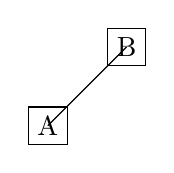
\begin{tikzpicture}[every node/.style={draw}]
  \draw (0,0) node {A} -- (1,1) node {B};
\end{tikzpicture}
\end{codeexample}
    \end{stylekey}
    %
    \begin{stylekey}{/tikz/every \meta{shape} node (initially \normalfont empty)}
        These styles are installed at the beginning of a node of a given
        \meta{shape}. For example, |every rectangle node| is used for rectangle
        nodes, and so on.
        %
\begin{codeexample}[]
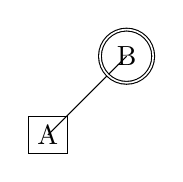
\begin{tikzpicture}
  [every rectangle node/.style={draw},
   every circle node/.style={draw,double}]
  \draw (0,0) node[rectangle] {A} -- (1,1) node[circle] {B};
\end{tikzpicture}
\end{codeexample}
    \end{stylekey}

    \begin{key}{/tikz/execute at begin node=\meta{code}}
        This option causes \meta{code} to be executed at the beginning of a
        node. Using this option multiple times will cause the code to
        accumulate.
    \end{key}

    \begin{key}{/tikz/execute at end node=\meta{code}}
        This option installs \meta{code} that will be executed at the end of
        the node. Using this option multiple times will cause the code to
        accumulate.
        %
\begin{codeexample}[]

\begin{tikzpicture}
  [execute at begin node={A},
   execute at end node={D}]
  \node[execute at begin node={B}] {C};
\end{tikzpicture}
\end{codeexample}
    %
    \end{key}

    \medskip
    \textbf{Name scopes.}
    It turns out that the name of a node can further be influenced using two
    keys:
    %
    \begin{key}{/tikz/name prefix=\meta{text} (initially \normalfont empty)}
        The value of this key is prefixed to every node inside the current
        scope. This includes both the naming of the node (via the |name| key or
        via the implicit |(|\meta{name}|)| syntax) as well as any referencing
        of the node. Outside the scope, the nodes can (and need to) be
        referenced using ``full name'' consisting of the prefix and the node
        name.

        The net effect of this is that you can set the name prefix at the
        beginning of a scope to some value and then use short and simple names
        for the nodes inside the scope. Later, outside the scope, you can
        reference the nodes via their full name:
        %
\begin{codeexample}[]
\tikz {
  \begin{scope}[name prefix = top-]
    \node (A) at (0,1) {A};
    \node (B) at (1,1) {B};
    \draw (A) -- (B);
  \end{scope}
  \begin{scope}[name prefix = bottom-]
    \node (A) at (0,0) {A};
    \node (B) at (1,0) {B};
    \draw (A) -- (B);
  \end{scope}

  \draw [red] (top-A) -- (bottom-B);
}
\end{codeexample}
        %
        As can be seen, name prefixing makes it easy to write reusable code.
    \end{key}
    %
    \begin{key}{/tikz/name suffix=\meta{text} (initially \normalfont empty)}
        Works as |name prefix|, only the \meta{text} is appended to every node
        name in the current scope.
    \end{key}
\end{pathoperation}

There is a special syntax for specifying ``light-weight'' nodes:

\begin{pathoperation}{coordinate}{\opt{|[|\meta{options}|]|}|(|\meta{name}|)|\opt{|at(|\meta{coordinate}|)|}}
    This has the same effect as

    |\node[shape=coordinate]|\verb|[|\meta{options}|](|\meta{name}|)at(|\meta{coordinate}|){}|,

    where the |at| part may be omitted.
\end{pathoperation}

Since nodes are often the only path operation on paths, there are two special
commands for creating paths containing only a node:

\begin{command}{\node}
    Inside |{tikzpicture}| this is an abbreviation for |\path node|.
\end{command}

\begin{command}{\coordinate}
    Inside |{tikzpicture}| this is an abbreviation for |\path coordinate|.
\end{command}


\subsubsection{Predefined Shapes}
\label{section-nodes-predefined}
\label{section-the-shapes}

\pgfname\ \todosp{why two labels for the same point? The first doesn't seem to
be used anywhere} and \tikzname\ define three shapes, by default:
%
\begin{itemize}
    \item |rectangle|,
    \item |circle|, and
    \item |coordinate|.
\end{itemize}
%
By loading library packages, you can define more shapes like ellipses or
diamonds; see Section~\ref{section-libs-shapes} for the complete list of
shapes.

\label{section-tikz-coordinate-shape}%
The |coordinate| shape is handled in a special way by \tikzname. When a node
|x| whose shape is |coordinate| is used as a coordinate |(x)|, this has the
same effect as if you had said |(x.center)|. None of the special ``line
shortening rules'' apply in this case. This can be useful since, normally, the
line shortening causes paths to be segmented and they cannot be used for
filling. Here is an example that demonstrates the difference:
%
\begin{codeexample}[]
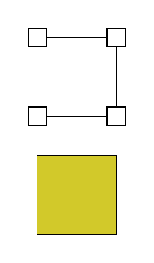
\begin{tikzpicture}[every node/.style={draw}]
  \path[yshift=1.5cm,shape=rectangle]
    (0,0) node(a1){} (1,0) node(a2){}
    (1,1) node(a3){} (0,1) node(a4){};
  \filldraw[fill=yellow!80!black] (a1) -- (a2) -- (a3) -- (a4);

  \path[shape=coordinate]
    (0,0) coordinate(b1) (1,0) coordinate(b2)
    (1,1) coordinate(b3) (0,1) coordinate(b4);
  \filldraw[fill=yellow!80!black] (b1) -- (b2) -- (b3) -- (b4);
\end{tikzpicture}
\end{codeexample}


\subsubsection{Common Options: Separations, Margins, Padding and
               Border Rotation}
\label{section-shape-seps}
\label{section-shape-common-options}

The \todosp{why two labels for the same point?} exact behavior of shapes
differs, shapes defined for more special purposes (like a, say, transistor
shape) will have even more custom behaviors. However, there are some options
that apply to most shapes:

\begin{key}{/pgf/inner sep=\meta{dimension} (initially .3333em)}
        \keyalias{tikz}
    An additional (invisible) separation space of \meta{dimension} will be
    added inside the shape, between the text and the shape's background path.
    The effect is as if you had added appropriate horizontal and vertical skips
    at the beginning and end of the text to make it a bit ``larger''.

    For those familiar with \textsc{css}, this is the same as \emph{padding}.
    %
\begin{codeexample}[]
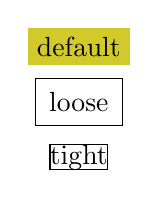
\begin{tikzpicture}
  \draw (0,0)     node[inner sep=0pt,draw] {tight}
        (0cm,2em) node[inner sep=5pt,draw] {loose}
        (0cm,4em) node[fill=yellow!80!black]   {default};
\end{tikzpicture}
\end{codeexample}
    %
\end{key}

\begin{key}{/pgf/inner xsep=\meta{dimension} (initially .3333em)}
        \keyalias{tikz}
    Specifies the inner separation in the $x$-direction, only.
\end{key}

\begin{key}{/pgf/inner ysep=\meta{dimension} (initially .3333em)}
        \keyalias{tikz}
    Specifies the inner separation in the $y$-direction, only.
\end{key}

\begin{key}{/pgf/outer sep=\meta{dimension or ``auto''}}
        \keyalias{tikz}
    This option adds an additional (invisible) separation space of
    \meta{dimension} outside the background path. The main effect of this
    option is that all anchors will move a little ``to the outside''.

    For those familiar with \textsc{css}, this is same as \emph{margin}.

    The default for this option is half the line width. When the default is
    used and when the background path is draw, the anchors will lie exactly on
    the ``outside border'' of the path (not on the path itself).
    %
\begin{codeexample}[]
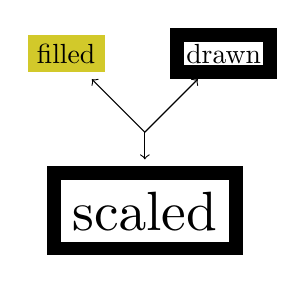
\begin{tikzpicture}
  \draw[line width=5pt]
    (0,0)  node[fill=yellow!80!black] (f) {filled}
    (2,0)  node[draw]                 (d) {drawn}
    (1,-2) node[draw,scale=2]         (s) {scaled};

  \draw[->] (1,-1) -- (f);
  \draw[->] (1,-1) -- (d);
  \draw[->] (1,-1) -- (s);
\end{tikzpicture}
\end{codeexample}

    As the above example demonstrates, the standard settings for the outer sep
    are not always ``correct''. First, when a shape is filled, but not drawn,
    the outer sep should actually be |0|. Second, when a node is scaled, for
    instance by a factor of 5, the outer separation also gets scaled by a
    factor of 5, while the line width stays at its original width; again
    causing problems.

    In such cases, you can say |outer sep=auto| to make \tikzname\ \emph{try}
    to compensate for the effects described above. This is done by, firstly,
    setting the outer sep to |0| when no drawing is done and, secondly, setting
    the outer separations to half the line width (as before) times two
    adjustment factors, one for the horizontal separations and one for the
    vertical separations (see Section~\ref{section-adjustment-transformations}
    for details on these factors). Note, however, that these factors can
    compensate only for transformations that are either scalings plus rotations
    or scalings with different magnitudes in the horizontal and the vertical
    direction. If you apply slanting, the factors will only approximate the
    correct values.

    In general, it is a good idea to say |outer sep=auto| at some early stage.
    It is not the default mainly for compatibility with earlier versions.
    %
\begin{codeexample}[]
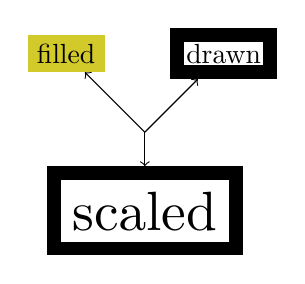
\begin{tikzpicture}[outer sep=auto]
  \draw[line width=5pt]
    (0,0)  node[fill=yellow!80!black] (f) {filled}
    (2,0)  node[draw]                 (d) {drawn}
    (1,-2) node[draw,scale=2]         (s) {scaled};

  \draw[->] (1,-1) -- (f);
  \draw[->] (1,-1) -- (d);
  \draw[->] (1,-1) -- (s);
\end{tikzpicture}
\end{codeexample}
    %
\end{key}

\begin{key}{/pgf/outer xsep=\meta{dimension} (initially .5\string\pgflinewidth)}
        \keyalias{tikz}
    Specifies the outer separation in the $x$-direction, only. This value will
    be overwritten when |outer sep| is set, either to the value given there or
    a computed value in case of |auto|.
\end{key}

\begin{key}{/pgf/outer ysep=\meta{dimension} (initially .5\string\pgflinewidth)}
        \keyalias{tikz}
    Specifies the outer separation in the $y$-direction, only.
\end{key}

\begin{key}{/pgf/minimum height=\meta{dimension} (initially 1pt)}
        \keyalias{tikz}
    This option ensures that the height of the shape (including the inner, but
    ignoring the outer separation) will be at least \meta{dimension}. Thus, if
    the text plus the inner separation is not at least as large as
    \meta{dimension}, the shape will be enlarged appropriately. However, if the
    text is already larger than \meta{dimension}, the shape will not be shrunk.
    %
\begin{codeexample}[]
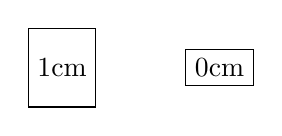
\begin{tikzpicture}
  \draw (0,0) node[minimum height=1cm,draw] {1cm}
        (2,0) node[minimum height=0cm,draw] {0cm};
\end{tikzpicture}
\end{codeexample}
    %
\end{key}

\begin{key}{/pgf/minimum width=\meta{dimension} (initially 1pt)}
        \keyalias{tikz}
    Same as |minimum height|, only for the width.
    %
\begin{codeexample}[]
\begin{tikzpicture}
  \draw (0,0) node[minimum height=2cm,minimum width=3cm,draw] {$3 \times 2$};
\end{tikzpicture}
\end{codeexample}
    %
\end{key}

\begin{key}{/pgf/minimum size=\meta{dimension}}
        \keyalias{tikz}
    Sets both the minimum height and width at the same time.
    %
\begin{codeexample}[]
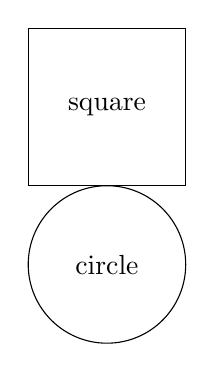
\begin{tikzpicture}
  \draw (0,0)  node[minimum size=2cm,draw] {square};
  \draw (0,-2) node[minimum size=2cm,draw,circle] {circle};
\end{tikzpicture}
\end{codeexample}
    %
\end{key}

\begin{key}{/pgf/shape aspect=\meta{aspect ratio} (initially none)}
        \keyalias{tikz}
    Sets a desired aspect ratio for the shape. For the |diamond| shape, this
    option sets the ratio between width and height of the shape. Unlike
    |/pgf/aspect| which only recommends the ratio, this key ensures it.

    If the special value |none| is given, the ratio assurance is canceled.
    %
\begin{codeexample}[preamble={\usetikzlibrary{shapes.geometric}}]
\begin{tikzpicture}
  \draw (0,0)  node[shape aspect=1,diamond,draw] {aspect 1};
  \draw (0,-2) node[shape aspect=2,diamond,draw] {aspect 2};
\end{tikzpicture}
\end{codeexample}
    %
\end{key}

    \label{section-rotating-shape-borders}

Some shapes (but not all), support a special kind of rotation. This rotation
affects only the border of a shape and is independent of the node contents, but
\emph{in addition} to any other transformations.
%
\begin{codeexample}[preamble={\usetikzlibrary{shapes.geometric}}]
\tikzset{every node/.style={dart, shape border uses incircle,
  inner sep=1pt, draw}}
\tikz \node foreach \a/\b/\c in {A/0/0, B/45/0, C/0/45, D/45/45}
            [shape border rotate=\b, rotate=\c] at (\b/36,-\c/36) {\a};
\end{codeexample}

There are two types of rotation: restricted and unrestricted. Which type of
rotation is applied is determined by on how the shape border is constructed. If
the shape border is constructed using an incircle, that is, a circle that
tightly fits the node contents (including the |inner sep|), then the rotation
can be unrestricted. If, however, the border is constructed using the natural
dimensions of the node contents, the rotation is restricted to integer
multiples of 90 degrees.

Why should there be two kinds of rotation and border construction? Borders
constructed using the natural dimensions of the node contents provide a much
tighter fit to the node contents, but to maintain this tight fit, the border
rotation must be restricted to integer multiples of 90 degrees. By using an
incircle, unrestricted rotation is possible, but the border will not make a
very tight fit to the node contents.
%
\begin{codeexample}[preamble={\usetikzlibrary{shapes.geometric}}]
\tikzset{every node/.style={isosceles triangle, draw}}
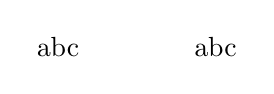
\begin{tikzpicture}
  \node {abc};
  \node [shape border uses incircle] at (2,0) {abc};
\end{tikzpicture}
\end{codeexample}

There are \pgfname{} keys that determine how a shape border is constructed, and
to specify its rotation. It should be noted that not all shapes support these
keys, so reference should be made to the documentation for individual shapes.

\begin{key}{/pgf/shape border uses incircle=\opt{\meta{boolean}} (default true)}
        \keyalias{tikz}
    Determines if the border of a shape is constructed using the incircle. If
    no value is given \meta{boolean} will take the default value |true|.
\end{key}

\begin{key}{/pgf/shape border rotate=\meta{angle} (initially 0)}
        \keyalias{tikz}
    Rotates the border of a shape independently of the node contents, but in
    addition to any other transformations. If the shape border is not
    constructed using the incircle, the rotation will be rounded to the nearest
    integer multiple of 90 degrees when the shape is drawn.
\end{key}

Note that if the border of the shape is rotated, the compass point anchors, and
`text box' anchors (including |mid east|, |base west|, and so on), \emph{do not
rotate}, but the other anchors do:
%
\begin{codeexample}[preamble={\usetikzlibrary{shapes.geometric}}]
\tikzset{every node/.style={shape=trapezium, draw, shape border uses incircle}}
\begin{tikzpicture}
  \node at (0,0)  (A) {A};
  \node [shape border rotate=30] at (1.5,0) (B) {B};
  \foreach \s/\t in
    {left side/base east, bottom side/north, bottom left corner/base}{
       \fill[red]  (A.\s) circle(1.5pt) (B.\s) circle(1.5pt);
       \fill[blue] (A.\t) circle(1.5pt) (B.\t) circle(1.5pt);
  }
\end{tikzpicture}
\end{codeexample}

Finally, a somewhat unfortunate side-effect of rotating shape borders is that
the supporting shapes do not distinguish between |outer xsep| and |outer ysep|,
and typically, the larger of the two values will be used.


\subsection{Multi-Part Nodes}
\label{section-nodes-multi}

Most nodes just have a single simple text label. However, nodes of a more
complicated shape might be made up from several \emph{node parts}. For example,
in automata theory a so-called Moore state has a state name, drawn in the upper
part of the state circle, and an output text, drawn in the lower part of the
state circle. These two parts are quite independent. Similarly, a \textsc{uml}
class shape would have a name part, a method part, and an attributes part.
Different molecule shapes might use parts for the different atoms to be drawn
at the different positions, and so on.

Both \pgfname\ and \tikzname\ support such multipart nodes. On the lower level,
\pgfname\ provides a system for specifying that a shape consists of several
parts. On the \tikzname\ level, you specify the different node parts by using
the following command:

\begin{command}{\nodepart\opt{|[|\meta{options}|]|}\marg{part name}}
    This command can only be used inside the \meta{text} argument of a |node|
    path operation. It works a little bit like a |\part| command in \LaTeX. It
    will stop the typesetting of whatever node part was typeset until now and
    then start putting all following text into the node part named \meta{part
    name} -- until another |\partname| is encountered or until the node
    \meta{text} ends. The \meta{options} will be local to this part.
    %
\begin{codeexample}[preamble={\usetikzlibrary{shapes.multipart}}]
\begin{tikzpicture}
  \node [circle split,draw,double,fill=red!20]
  {
    % No \nodepart has been used, yet. So, the following is put in the
    % ``text'' node part by default.
    $q_1$
    \nodepart{lower} % Ok, end ``text'' part, start ``output'' part
    $00$
  }; % output part ended.
\end{tikzpicture}
\end{codeexample}

    You will have to lookup which parts are defined by a shape.

    The following styles influences node parts:
    %
    \begin{stylekey}{/tikz/every \meta{part name} node part (initially \normalfont empty)}
        This style is installed at the beginning of every node part named
        \meta{part name}.
        %
\begin{codeexample}[preamble={\usetikzlibrary{shapes.multipart}}]
\tikz [every lower node part/.style={red}]
  \node [circle split,draw] {$q_1$ \nodepart{lower} $00$};
\end{codeexample}
    \end{stylekey}
\end{command}


\subsection{The Node Text}
\label{section-nodes-options}

\subsubsection{Text Parameters: Color and Opacity}

The simplest option for the text in nodes is its color. Normally, this color is
just the last color installed using |color=|, possibly inherited from another
scope. However, it is possible to specifically set the color used for text
using the following option:

\begin{key}{/tikz/text=\meta{color}}
    Sets the color to be used for text labels. A |color=| option will
    immediately override this option.
    %
\begin{codeexample}[]
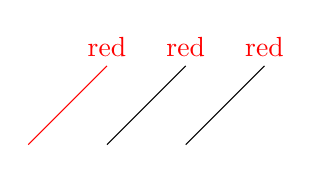
\begin{tikzpicture}
  \draw[red]       (0,0) -- +(1,1) node[above]     {red};
  \draw[text=red]  (1,0) -- +(1,1) node[above]     {red};
  \draw            (2,0) -- +(1,1) node[above,red] {red};
\end{tikzpicture}
\end{codeexample}
    %
\end{key}

Just like the color itself, you may also wish to set the opacity of the text
only. For this, use the |text opacity| option, which is detailed in
Section~\ref{section-tikz-transparency}.


\subsubsection{Text Parameters: Font}

Next, you may wish to adjust the font used for the text. Naturally, you can
just use a font command like |\small| or |\rm| at the beginning of a node.
However, the following two options make it easier to set the font used in nodes
on a general basis. Let us start with:

\begin{key}{/tikz/node font=\meta{font commands}}
    This option sets the font used for all text used in a node.
    %
\begin{codeexample}[]
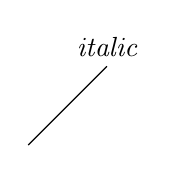
\begin{tikzpicture}
  \draw[node font=\itshape] (1,0) -- +(1,1) node[above] {italic};
\end{tikzpicture}
\end{codeexample}
    %
    Since the \meta{font commands} are executed at a very early stage in the
    construction of the node, the font selected using this command will also
    dictate the values of dimensions defined in terms of |em| or |ex|. For
    instance, when the |minimum height| of a node is |3em|, the actual height
    will be (at least) three times the line distance selected by the \meta{font
    commands}:
\begin{codeexample}[]
\tikz \node [node font=\tiny,  minimum height=3em, draw] {tiny};
\tikz \node [node font=\small, minimum height=3em, draw] {small};
\end{codeexample}
    %
\end{key}

The other font command is:
%
\begin{key}{/tikz/font=\meta{font commands}}
    Sets the font used for the text inside nodes. However, this font will
    \emph{not} (yet) be installed when any of the dimensions of the node are
    being computed, so dimensions like |1em| will be with respect to the font
    used outside the node (usually the font that was in force when the picture
    started).
    %
\begin{codeexample}[]

\begin{tikzpicture}
  \node [font=\itshape] {italic};
\end{tikzpicture}
\end{codeexample}

\begin{codeexample}[]
\tikz \node [font=\tiny,  minimum height=3em, draw] {tiny};
\tikz \node [font=\small, minimum height=3em, draw] {small};
\end{codeexample}

    A useful example of how the |font| option can be used is the following:
    %
\begin{codeexample}[preamble={\usetikzlibrary{shapes.multipart}}]
\tikz [every text node part/.style={font=\itshape},
       every lower node part/.style={font=\footnotesize}]
  \node [circle split,draw] {state \nodepart{lower} output};
\end{codeexample}

    As can be seen, the font can be changed for each node part. This does
    \emph{not} work with the |node font| command since, as the name suggests,
    this command can only be used to select the ``overall'' font for the node
    and this is done very early.
\end{key}


\subsubsection{Text Parameters: Alignment and Width for Multi-Line Text}

Normally, when a node is typeset, all the text you give in the braces is put in
one long line (in an |\hbox|, to be precise) and the node will become as wide
as necessary.

From time to time you may wish to create nodes that contain multiple lines of
text. There are three different ways of achieving this:
%
\begin{enumerate}
    \item Inside the node, you can put some standard environment that produces
        multi-line, aligned text. For instance, you can use a |{tabular}|
        inside a node:
        %
\begin{codeexample}[width=5cm]
\tikz \node [draw] {
  \begin{tabular}{cc}
    upper left & upper right\\
    lower left & lower right
  \end{tabular}
};
\end{codeexample}
        %
        This approach offers the most flexibility in the sense that it allows
        you to use all of the alignment commands offered by your format of
        choice.
    \item You use |\\| inside your node to mark the end of lines and then
        request \tikzname\ to arrange these lines in some manner. This will
        only be done, however, if the |align| option has been given.
        %
\begin{codeexample}[]
\tikz[align=left] \node[draw] {This is a\\demonstration.};
\end{codeexample}
        %
\begin{codeexample}[]
\tikz[align=center] \node[draw] {This is a\\demonstration.};
\end{codeexample}
        %
        The |\\| command takes an optional extra space as an argument in square
        brackets.
        %
\begin{codeexample}[]
\tikz \node[fill=yellow!80!black,align=right]
  {This is a\\[-2pt] demonstration text for\\[1ex] alignments.};
\end{codeexample}
        %
    \item You can request that \tikzname\ does an automatic line-breaking for
        you inside the node by specifying a fixed |text width| for the node. In
        this case, you can still use |\\| to enforce a line-break. Note that
        when you specify a text width, the node will have this width,
        independently of whether the text actually ``reaches the end'' of the
        node.
\end{enumerate}

Let us now first have a look at the |text width| command.
    %
\begin{key}{/tikz/text width=\meta{dimension}}
    This option will put the text of a node in a box of the given width
    (something akin to a |{minipage}| of this width, only portable across
    formats). If the node text is not as wide as \meta{dimension}, it will
    nevertheless be put in a box of this width. If it is larger, line breaking
    will be done.

    By default, when this option is given, a ragged right border will be used
    (|align=left|). This is sensible since, typically, these boxes are narrow
    and justifying the text looks ugly. You can, however, change the alignment
    using |align| or directly using commands line |\centering|.
    %
\begin{codeexample}[]
\tikz \draw (0,0) node[fill=yellow!80!black,text width=3cm]
  {This is a demonstration text for showing how line breaking works.};
\end{codeexample}
    %
    Setting \meta{dimension} to an empty string causes the automatic line
    breaking to be disabled.
\end{key}

\begin{key}{/tikz/align=\meta{alignment option}}
    This key is used to set up an alignment for multi-line text inside a node.
    If |text width| is set to some width (let us call this \emph{alignment with
    line breaking}), the |align| key will setup the |\leftskip| and the
    |\rightskip| in such a way that the text is broken and aligned according to
    \meta{alignment option}. If |text width| is not set (that is, set to the
    empty string; let us call this \emph{alignment without line breaking}),
    then a different mechanism is used internally, namely the key
    |node halign header|, is set to an appropriate value. While this key, which
    is documented below, is not to be used by beginners, the net effect is
    simple: When |text width| is not set, you can use |\\| to break lines and
    align them according to \meta{alignment option} and the resulting node's
    width will be minimal to encompass the resulting lines.

    In detail, you can set \meta{alignment option} to one of the following values:
    %
    \begin{description}
        \item[|align=|\declare{|left|}] For alignment without line breaking,
            the different lines are simply aligned such that their left borders
            are below one another.
            %
\begin{codeexample}[]
\tikz \node[fill=yellow!80!black,align=left]
  {This is a\\ demonstration text for\\ alignments.};
\end{codeexample}
            %
            For alignment with line breaking, the same will happen; only the
            lines will now, additionally, be broken automatically:
            %
\begin{codeexample}[]
\tikz \node[fill=yellow!80!black,text width=3cm,align=left]
  {This is a demonstration text for showing how line breaking works.};
\end{codeexample}
            %
        \item[|align=|\declare{\texttt{flush left}}] For alignment without line
            breaking this option has exactly the same effect as |left|.
            However, for alignment with line breaking, there is a difference:
            While |left| uses the original plain \TeX\ definition of a ragged
            right border, in which \TeX\ will try to balance the right border
            as well as possible, |flush left| causes the right border to be
            ragged in the \LaTeX-style, in which no balancing occurs. This
            looks ugly, but it may be useful for very narrow boxes and when you
            wish to avoid hyphenations.
            %
\begin{codeexample}[]
\tikz \node[fill=yellow!80!black,text width=3cm,align=flush left]
  {This is a demonstration text for showing how line breaking works.};
\end{codeexample}
            %
        \item[|align=|\declare{|right|}] Works like |left|, only for right
            alignment.
            %
\begin{codeexample}[]
\tikz \node[fill=yellow!80!black,align=right]
  {This is a\\ demonstration text for\\ alignments.};
\end{codeexample}
            %
\begin{codeexample}[]
\tikz \node[fill=yellow!80!black,text width=3cm,align=right]
  {This is a demonstration text for showing how line breaking works.};
\end{codeexample}
            %
        \item[|align=|\declare{\texttt{flush right}}] Works like |flush left|,
            only for right alignment.
            %
\begin{codeexample}[]
\tikz \node[fill=yellow!80!black,text width=3cm,align=flush right]
  {This is a demonstration text for showing how line breaking works.};
\end{codeexample}
            %
        \item[|align=|\declare{|center|}] Works like |left| or |right|, only
            for centered alignment.
            %
\begin{codeexample}[]
\tikz \node[fill=yellow!80!black,align=center]
  {This is a\\ demonstration text for\\ alignments.};
\end{codeexample}
\begin{codeexample}[]
\tikz \node[fill=yellow!80!black,text width=3cm,align=center]
  {This is a demonstration text for showing how line breaking works.};
\end{codeexample}

            There is one annoying problem with the |center| alignment (but not
            with |flush center| and the other options): If you specify a large
            line width and the node text fits on a single line and is, in fact,
            much shorter than the specified |text width|, an underfull
            horizontal box will result. Unfortunately, this cannot be avoided,
            due to the way \TeX\ works (more precisely, I have thought long and
            hard about this and have not been able to figure out a sensible way
            to avoid this). For this reason, \tikzname\ switches off horizontal
            badness warnings inside boxes with |align=center|. Since this will
            also suppress some ``wanted'' warnings, there is also an option for
            switching the warnings on once more:
            %
            \begin{key}{/tikz/badness warnings for centered text=\meta{true or false} (initially false)}
                If set to true, normal badness warnings will be issued for
                centered boxes. Note that you may get annoying warnings for
                perfectly normal boxes, namely whenever the box is very large
                and the contents is not long enough to fill the box
                sufficiently.
            \end{key}
        \item[|align=|\declare{\texttt{flush center}}] Works like |flush left|
            or |flush right|, only for center alignment. Because of all the
            trouble that results from the |center| option in conjunction with
            narrow lines, I suggest picking this option rather than  |center|
            \emph{unless} you have longer text, in which case |center| will
            give the typographically better results.
            %
\begin{codeexample}[]
\tikz \node[fill=yellow!80!black,text width=3cm,align=flush center]
  {This is a demonstration text for showing how line breaking works.};
\end{codeexample}
            %
        \item[|align=|\declare{|justify|}] For alignment without line breaking,
            this has the same effect as |left|. For alignment with line
            breaking, this causes the text to be ``justified''. Use this only
            with rather broad nodes.
{%
\hbadness=10000
\begin{codeexample}[]
\tikz \node[fill=yellow!80!black,text width=3cm,align=justify]
  {This is a demonstration text for showing how line breaking works.};
\end{codeexample}
}
            In the above example, \TeX\ complains (rightfully) about three very
            badly typeset lines. (For this manual I asked \TeX\ to stop
            complaining by using |\hbadness=10000|, but this is a foul deed,
            indeed.)
        \item[|align=|\declare{|none|}] Disables all alignments and |\\| will
            not be redefined.
    \end{description}
\end{key}

\begin{key}{/tikz/node halign header=\meta{macro storing a header} (initially \normalfont empty)}
    This is the key that is used by |align| internally for alignment without
    line breaking. Read the following only if you are familiar with the
    |\halign| command.

    This key only has an effect if |text width| is empty, otherwise it is
    ignored. Furthermore, if \meta{macro storing a header} is empty, then this
    key also has no effect. So, suppose |text width| is empty, but
    \meta{header} is not. In this case the following happens:

    When the node text is parsed, the command |\\| is redefined internally.
    This redefinition is done in such a way that the text from the start of the
    node to the first occurrence of |\\| is put in an |\hbox|. Then the text
    following |\\| up to the next |\\| is put in another |\hbox|. This goes on
    until the text between the last |\\| and the closing |}| is also put in an
    |\hbox|.

    The \meta{macro storing a header} should be a macro that contains some text
    suitable for use as a header for the |\halign| command. For instance, you
    might define
    %
\begin{codeexample}[code only]
\def\myheader{\hfil\hfil##\hfil\cr}
\tikz [node halign header=\myheader] ...
\end{codeexample}
    %
    You cannot just say |node halign header=\hfil\hfil#\hfil\cr| because this
    confuses \TeX\ inside matrices, so this detour via a macro is needed.

    Next, conceptually, all these boxes are recursively put inside an |\halign|
    command. Assuming that \meta{first} is the first of the above boxes, the
    command |\halign{|\meta{header} |\box|\meta{first} |\cr}| is used to create
    a new box, which we will call the \meta{previous box}. Then, the following
    box is created, where \meta{second} is the second input box:
    |\halign{|\meta{header} |\box|\meta{previous box} |\cr|
    |\box|\meta{second}|\cr}|. Let us call the resulting box the \meta{previous
    box} once more. Then the next box that is created is
    |\halign{|\meta{header} |\box|\meta{previous box} |\cr|
    |\box|\meta{third}|\cr}|.

    All of this means that if \meta{header} is an |\halign| header like
    |\hfil#\hfil\cr|, then all boxes will be centered relative to one another.
    Similarly, a \meta{header} of |\hfil#\cr| causes the text to be flushed
    right.

    Note that this mechanism is not flexible enough to all multiple columns
    inside \meta{header}. You will have to use a |tabular| or a |matrix| in
    such cases.

    One further note: Since the text of each line is placed in a box, settings
    will be local to each ``line''. This is very similar to the way a cell in a
    |tabular| or a |matrix| behaves.
\end{key}


\subsubsection{Text Parameters: Height and Depth of Text}

In addition to changing the width of nodes, you can also change the height of
nodes. This can be done in two ways: First, you can use the option
|minimum height|, which ensures that the height of the whole node is at least
the given height (this option is described in more detail later). Second, you
can use the option |text height|, which sets the height of the text itself,
more precisely, of the \TeX\ text box of the text. Note that the |text height|
typically is not the height of the shape's box: In addition to the
|text height|, an internal |inner sep| is added as extra space and the text
depth is also taken into account.

I recommend using |minimum size| instead of |text height| except for special
situations.

\begin{key}{/tikz/text height=\meta{dimension}}
    Sets the height of the text boxes in shapes. Thus, when you write something
    like |node {text}|, the |text| is first typeset, resulting in some box of a
    certain height. This height is then replaced by the height |text height|.
    The resulting box is then used to determine the size of the shape, which
    will typically be larger. When you write |text height=| without specifying
    anything, the ``natural'' size of the text box remains unchanged.
    %
\begin{codeexample}[]
\tikz \node[draw]                  {y};
\tikz \node[draw,text height=10pt] {y};
\end{codeexample}
    %
\end{key}

\begin{key}{/tikz/text depth=\meta{dimension}}
    This option works like |text height|, only for the depth of the text box.
    This option is mostly useful when you need to ensure a uniform depth of
    text boxes that need to be aligned.
\end{key}


\subsection{Positioning Nodes}
\label{section-nodes-anchors}

When you place a node at some coordinate, the node is centered on this
coordinate by default. This is often undesirable and it would be better to have
the node to the right or above the actual coordinate.


\subsubsection{Positioning Nodes Using Anchors}

\pgfname\ uses a so-called anchoring mechanism to give you a very fine control
over the placement. The idea is simple: Imagine a node of rectangular shape of
a certain size. \pgfname\ defines numerous anchor positions in the shape. For
example to upper right corner is called, well, not ``upper right anchor'', but
the |north east| anchor of the shape. The center of the shape has an anchor
called |center| on top of it, and so on. Here are some examples (a complete
list is given in Section~\ref{section-the-shapes}).

\medskip\noindent
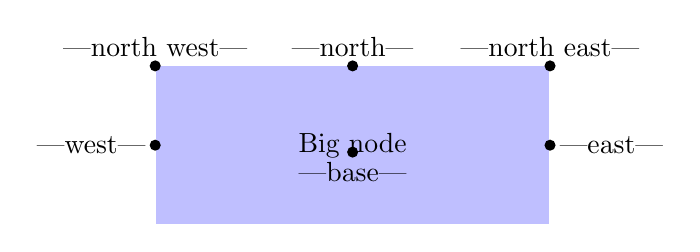
\begin{tikzpicture}
  \path node[minimum height=2cm,minimum width=5cm,fill=blue!25](x) {Big node};
  \fill (x.north)      circle (2pt) node[above] {|north|}
        (x.north east) circle (2pt) node[above] {|north east|}
        (x.north west) circle (2pt) node[above] {|north west|}
        (x.west) circle (2pt)       node[left]  {|west|}
        (x.east) circle (2pt)       node[right] {|east|}
        (x.base) circle (2pt)       node[below] {|base|};
\end{tikzpicture}

Now, when you place a node at a certain coordinate, you can ask \tikzname\ to
place the node shifted around in such a way that a certain anchor is at the
coordinate. In the following example, we ask \tikzname\ to shift the first node
such that its  |north east| anchor is at coordinate |(0,0)| and that the |west|
anchor of the second node is at coordinate |(1,1)|.
%
\begin{codeexample}[]
\tikz \draw           (0,0) node[anchor=north east] {first node}
            rectangle (1,1) node[anchor=west] {second node};
\end{codeexample}

Since the default anchor is |center|, the default behavior is to shift the node
in such a way that it is centered on the current position.

\begin{key}{/tikz/anchor=\meta{anchor name}}
    Causes the node to be shifted such that its anchor \meta{anchor name} lies
    on the current coordinate.

    The only anchor that is present in all shapes is |center|. However, most
    shapes will at least define anchors in all ``compass directions''.
    Furthermore, the standard shapes also define a |base| anchor, as well as
    |base west| and |base east|, for placing things on the baseline of the
    text.

    The standard shapes also define a |mid| anchor (and |mid west| and
    |mid east|). This anchor is half the height of the character ``x'' above
    the base line. This anchor is useful for vertically centering multiple
    nodes that have different heights and depth. Here is an example:
    %
\begin{codeexample}[]
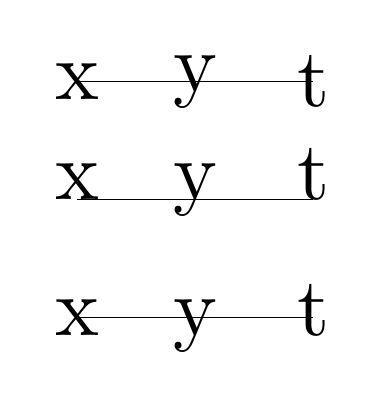
\begin{tikzpicture}[scale=3,transform shape]
  % First, center alignment -> wobbles
  \draw[anchor=center] (0,1)  node{x} -- (0.5,1)  node{y} -- (1,1)  node{t};
  % Second, base alignment -> no wobble, but too high
  \draw[anchor=base]   (0,.5) node{x} -- (0.5,.5) node{y} -- (1,.5) node{t};
  % Third, mid alignment
  \draw[anchor=mid]    (0,0)  node{x} -- (0.5,0)  node{y} -- (1,0)  node{t};
\end{tikzpicture}
\end{codeexample}
    %
\end{key}


\subsubsection{Basic Placement Options}

Unfortunately, while perfectly logical, it is often rather counter-intuitive
that in order to place a node \emph{above} a given point, you need to specify
the |south| anchor. For this reason, there are some useful options that allow
you to select the standard anchors more intuitively:

\begin{key}{/tikz/above=\meta{offset} (default 0pt)}
    Does the same as |anchor=south|. If the \meta{offset} is specified, the
    node is additionally shifted upwards by the given \meta{offset}.
    %
\begin{codeexample}[]
\tikz \fill (0,0) circle (2pt) node[above] {above};
\end{codeexample}
    %
\begin{codeexample}[]
\tikz \fill (0,0) circle (2pt) node[above=2pt] {above};
\end{codeexample}
    %
\end{key}

\begin{key}{/tikz/below=\meta{offset} (default 0pt)}
    Similar to |above|.
\end{key}

\begin{key}{/tikz/left=\meta{offset} (default 0pt)}
    Similar to |above|.
\end{key}

\begin{key}{/tikz/right=\meta{offset} (default 0pt)}
    Similar to |above|.
\end{key}

\begin{key}{/tikz/above left}
    Does the same as |anchor=south east|. Note that giving both |above| and
    |left| options does not have the same effect as |above left|, rather only
    the last |left| ``wins''. Actually, this option also takes an \meta{offset}
    parameter, but using this parameter without using the |positioning| library
    is deprecated. (The |positioning| library changes the meaning of this
    parameter to something more sensible.)
    %
\begin{codeexample}[]
\tikz \fill (0,0) circle (2pt) node[above left] {above left};
\end{codeexample}
    %
\end{key}

\begin{key}{/tikz/above right}
    Similar to  |above left|.
    %
\begin{codeexample}[]
\tikz \fill (0,0) circle (2pt) node[above right] {above right};
\end{codeexample}
    %
\end{key}

\begin{key}{/tikz/below left}
    Similar to |above left|.
\end{key}

\begin{key}{/tikz/below right}
    Similar to |above left|.
\end{key}

\begin{key}{/tikz/centered}
    A shorthand for |anchor=center|.
\end{key}

% A second set of options behaves similarly, namely the |above of|,
% |below of|, and so on options. They cause the same anchors to be set
% as the options without |of|, however, their parameter is different:
% You must provide the name of another node. The current node will then
% be placed, say, above this specified node at a distance given by the
% option |node distance|.
% \begin{key}{/tikz/above of=\meta{node}}
%   This option causes the node to be placed at the distance
%   |node distance| above of \meta{node}. The anchor is |center|.
% \begin{codeexample}[]
% \begin{tikzpicture}[node distance=1cm]
%   \draw[help lines] (0,0) grid (3,2);
%   \node (a)                    {a};
%   \node (b) [above of=a]       {b};
%   \node (c) [above of=b]       {c};
%   \node (d) [right of=c]       {d};
%   \node (e) [below right of=d] {e};
% \end{tikzpicture}
% \end{codeexample}
% \end{key}
%
% \begin{key}{/tikz/above left of=\meta{node}}
%   Works like |above of|, only the node is now put above and left. The
%   |node distance| is the Euclidean distance between the two nodes, not
%   the $L_1$-distance.
% \end{key}
%
% \begin{key}{/tikz/above right of=\meta{node}}
%   Works similarly.
% \end{key}
% \begin{key}{/tikz/left of=\meta{node}}
%   Works similarly.
% \end{key}
% \begin{key}{/tikz/right of=\meta{node}}
%   Works similarly.
% \end{key}
% \begin{key}{/tikz/below of=\meta{node}}
%   Works similarly.
% \end{key}
% \begin{key}{/tikz/below left of=\meta{node}}
%   Works similarly.
% \end{key}
% \begin{key}{/tikz/below right of=\meta{node}}
%   Works similarly.
% \end{key}
% \begin{key}{/tikz/node distance=\meta{dimension}}
%   Sets the distance between nodes that are placed using the
%   |... of| options. Note that this distance is the distance between
%   the centers of the nodes, not the distance between their borders.
% \end{key}


\subsubsection{Advanced Placement Options}

While the standard placement options suffice for simple cases, the
|positioning| library offers more convenient placement options.

\begin{tikzlibrary}{positioning}
    The library defines additional options for placing nodes conveniently. It
    also redefines the standard options like |above| so that they give you
    better control of node placement.
\end{tikzlibrary}

When this library is loaded, the options like |above| or |above left| behave
differently.

\begin{key}{/tikz/above=\opt{\meta{specification}} (default 0pt)}
    With the |positioning| library loaded, the |above| option does not take a
    simple \meta{dimension} as its parameter. Rather, it can (also) take a more
    elaborate \meta{specification} as parameter. This \meta{specification} has
    the following general form: It starts with an optional \meta{shifting part}
    and is followed by an optional \meta{of-part}. Let us start with the
    \meta{shifting part}, which can have three forms:
    %
    \begin{enumerate}
        \item It can simply be a \declare{\meta{dimension}} (or a mathematical
            expression that evaluates to a dimension) like |2cm| or
            |3cm/2+4cm|. In this case, the following happens: the node's anchor
            is set to |south| and the node is vertically shifted upwards by
            \meta{dimension}.
            %
\begin{codeexample}[]
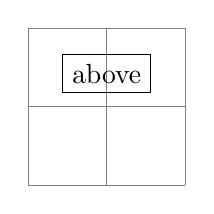
\begin{tikzpicture}
  \draw[help lines] (0,0) grid (2,2);
  \node at (1,1) [above=2pt+3pt,draw] {above};
\end{tikzpicture}
\end{codeexample}
            %
            This use of the |above| option is the same as if the |positioning|
            library were not loaded.
        \item It can be a \declare{\meta{number}} (that is, any mathematical
            expression that does not include a unit like |pt| or |cm|).
            Examples are |2| or |3+sin(60)|. In this case, the anchor is also
            set to |south| and the node is vertically shifted by the vertical
            component of the coordinate |(0,|\meta{number}|)|.
            %
\begin{codeexample}[]
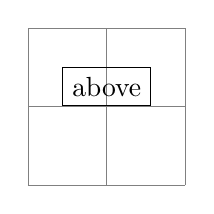
\begin{tikzpicture}
  \draw[help lines] (0,0) grid (2,2);
  \node at (1,1) [above=.2,draw] {above};
  % south border of the node is now 2mm above (1,1)
\end{tikzpicture}
\end{codeexample}
            %
        \item It can be of the form
            \declare{\meta{number or dimension 1}| and |\meta{number or dimension 2}}.
            This specification does not make particular sense for the |above|
            option, it is much more useful for options like |above left|. The
            reason it is allowed for the |above| option is that it is sometimes
            automatically used, as explained later.

            The effect of this option is the following. First, the point
            |(|\meta{number or dimension 2}|,|\meta{number or dimension 1}|)|
            is computed (note the inverted order), using the normal rules for
            evaluating such a coordinate, yielding some position. Then, the
            node is shifted by the vertical component of this point. The anchor
            is set to |south|.
            %
\begin{codeexample}[preamble={\usetikzlibrary{positioning}}]
\begin{tikzpicture}
  \draw[help lines] (0,0) grid (2,2);
  \node at (1,1) [above=.2 and 3mm,draw] {above};
  % south border of the node is also 2mm above (1,1)
\end{tikzpicture}
\end{codeexample}
    \end{enumerate}
    %
    The \meta{shifting part} can optionally be followed by a \meta{of-part},
    which has one of the following forms:
    %
    \begin{enumerate}
        \item The \meta{of-part} can be
            \declareandlabel{of}| |\meta{coordinate}, where \meta{coordinate} is
            \emph{not} in parentheses and it is \emph{not} just a node name. An
            example would be |of somenode.north| or |of {2,3}|. In this case, the
            following happens: First, the node's |at| parameter is set to the
            \meta{coordinate}. Second, the node is shifted according to the
            \meta{shift-part}. Third, the anchor is set to |south|.

            Here is a basic example:
            %
\begin{codeexample}[preamble={\usetikzlibrary{positioning}}]
\begin{tikzpicture}[every node/.style=draw]
  \draw[help lines] (0,0) grid (2,2);
  \node (somenode) at (1,1) {some node};

  \node [above=5mm of somenode.north east] {\tiny 5mm of somenode.north east};
  \node [above=1cm of somenode.north]      {\tiny 1cm of somenode.north};
\end{tikzpicture}
\end{codeexample}
            %
            As can be seen the |above=5mm of somenode.north east| option does,
            indeed, place the node 5mm above the north east anchor of
            |somenode|. The same effect could have been achieved writing
            |above=5mm| followed by |at=(somenode.north east)|.

            If the \meta{shifting-part} is missing, the shift is not zero, but
            rather the value of the |node distance| key is used, see below.
        \item The \meta{of-part} can be |of |\meta{node name}. An example would
            be |of somenode|. In this case, the following usually happens:
            %
            \begin{itemize}
                \item The anchor is set to |south|.
                \item The node is shifted according to the \meta{shifting part}
                    or, if it is missing, according to the value of
                    |node distance|.
                \item The node's |at| parameter is set to \meta{node
                    name}|.north|.
            \end{itemize}
            %
            The net effect of all this is that the new node will be placed in
            such a way that the distance between its south border and \meta{node
            name}'s north border is exactly the given distance.
            %
\begin{codeexample}[preamble={\usetikzlibrary{positioning}}]
\begin{tikzpicture}[every node/.style=draw]
  \draw[help lines] (0,0) grid (2,2);
  \node (some node) at (1,1) {some node};

  \node (other node) [above=1cm of some node] {\tiny above=1cm of some node};

  \draw [<->] (some node.north) -- (other node.south)
                                node [midway,right,draw=none] {1cm};
\end{tikzpicture}
\end{codeexample}
            %
            It is possible to change the behavior of this \meta{specification}
            rather drastically, using the following key:
            %
            \begin{key}{/tikz/on grid=\meta{boolean} (initially false)}
                When this key is set to |true|, an \meta{of-part} of the
                current form behaves differently: The anchors set for the
                current node as well as the anchor used for the other
                \meta{node name} are set to |center|.

                This has the following effect: When you say
                |above=1cm of somenode| with |on grid| set to true, the new
                node will be placed in such a way that its center is 1cm above
                the center of |somenode|. Repeatedly placing nodes in this way
                will result in nodes that are centered on ``grid coordinate'',
                hence the name of the option.
                %
\begin{codeexample}[preamble={\usetikzlibrary{positioning}}]
\begin{tikzpicture}[every node/.style=draw]
  \draw[help lines] (0,0) grid (2,3);

  % Not gridded
  \node (a1) at (0,0) {not gridded};
  \node (b1) [above=1cm of a1] {fooy};
  \node (c1) [above=1cm of b1] {a};

  % gridded
  \node (a2) at (2,0) {gridded};
  \node (b2) [on grid,above=1cm of a2] {fooy};
  \node (c2) [on grid,above=1cm of b2] {a};
\end{tikzpicture}
\end{codeexample}
            \end{key}
    \end{enumerate}

    \begin{key}{/tikz/node distance=\meta{shifting part} (initially 1cm and 1cm)}
        The value of this key is used as \meta{shifting part} is used if and
        only if a \meta{of-part} is present, but no \meta{shifting part}.
        %
\begin{codeexample}[preamble={\usetikzlibrary{positioning}}]
\begin{tikzpicture}[every node/.style=draw,node distance=5mm]
  \draw[help lines] (0,0) grid (2,3);

  % Not gridded
  \node (a1) at (0,0) {not gridded};
  \node (b1) [above=of a1] {fooy};
  \node (c1) [above=of b1] {a};

  % gridded
  \begin{scope}[on grid]
    \node (a2) at (2,0) {gridded};
    \node (b2) [above=of a2] {fooy};
    \node (c2) [above=of b2] {a};
  \end{scope}
\end{tikzpicture}
\end{codeexample}
    \end{key}
\end{key}

\begin{key}{/tikz/below=\opt{\meta{specification}}}
    This key is redefined in the same manner as |above|.
\end{key}

\begin{key}{/tikz/left=\opt{\meta{specification}}}
    This key is redefined in the same manner as |above|, only all vertical
    shifts are replaced by horizontal shifts.
\end{key}

\begin{key}{/tikz/right=\opt{\meta{specification}}}
    This key is redefined in the same manner as |left|.
\end{key}

\begin{key}{/tikz/above left=\opt{\meta{specification}}}
    This key is also redefined in a manner similar to the above, but behavior
    of the \meta{shifting part} is more complicated:
    %
    \begin{enumerate}
        \item When the \meta{shifting part} is of the form
            \meta{number or dimension}| and |\meta{number or dimension}, it has
            (essentially) the effect of shifting the node vertically upwards by
            the first \meta{number or dimension} and to the left by the second.
            To be more precise, the coordinate |(|\meta{second number or
            dimension}|,|\meta{first number or dimension}|)| is computed and
            then the node is shifted vertically by the $y$-part of the
            resulting coordinate and horizontally be the negated $x$-part of
            the result. (This is exactly what you expect, except possibly when
            you have used the |x| and |y| options to modify the |xy|-coordinate
            system so that the unit  vectors no longer point in the expected
            directions.)
        \item When the \meta{shifting part} is of the form \meta{number or
            dimension}, the node is shifted by this \meta{number or dimension}
            in the direction of $135^\circ$. This means that there is a
            difference between a \meta{shifting part} of |1cm| and of
            |1cm and 1cm|: In the second case, the node is shifted by 1cm
            upward and 1cm to the left; in the first case it is shifted by
            $\frac{1}{2}\sqrt{2}$cm upward and by the same amount to the left.
            A more mathematical way of phrasing this is the following: A plain
            \meta{dimension} is measured in the $l_2$-norm, while a
            \meta{dimension}| and |\meta{dimension} is measured in the
            $l_1$-norm.
    \end{enumerate}
    %
    The following example should help to illustrate the difference:
    %
\begin{codeexample}[preamble={\usetikzlibrary{positioning}}]
\begin{tikzpicture}[every node/.style={draw,circle}]
  \draw[help lines] (0,0) grid (2,5);
  \begin{scope}[node distance=5mm and 5mm]
    \node (b) at (1,4) {b};
    \node [left=of b] {1};       \node [right=of b] {2};
    \node [above=of b] {3};      \node [below=of b] {4};
    \node [above left=of b] {5}; \node [above right=of b] {6};
    \node [below left=of b] {7}; \node [below right=of b] {8};
  \end{scope}
  \begin{scope}[node distance=5mm]
    \node (a) at (1,1) {a};
    \node [left=of a] {1};       \node [right=of a] {2};
    \node [above=of a] {3};      \node [below=of a] {4};
    \node [above left=of a] {5}; \node [above right=of a] {6};
    \node [below left=of a] {7}; \node [below right=of a] {8};
  \end{scope}
\end{tikzpicture}
\end{codeexample}
    %
\begin{codeexample}[preamble={\usetikzlibrary{positioning}}]
\begin{tikzpicture}[every node/.style={draw,rectangle}]
  \draw[help lines] (0,0) grid (2,5);
  \begin{scope}[node distance=5mm and 5mm]
    \node (b) at (1,4) {b};
    \node [left=of b] {1};       \node [right=of b] {2};
    \node [above=of b] {3};      \node [below=of b] {4};
    \node [above left=of b] {5}; \node [above right=of b] {6};
    \node [below left=of b] {7}; \node [below right=of b] {8};
  \end{scope}
  \begin{scope}[node distance=5mm]
    \node (a) at (1,1) {a};
    \node [left=of a] {1};       \node [right=of a] {2};
    \node [above=of a] {3};      \node [below=of a] {4};
    \node [above left=of a] {5}; \node [above right=of a] {6};
    \node [below left=of a] {7}; \node [below right=of a] {8};
  \end{scope}
\end{tikzpicture}
\end{codeexample}
    %
\begin{codeexample}[preamble={\usetikzlibrary{positioning}}]
\begin{tikzpicture}[every node/.style={draw,rectangle},on grid]
  \draw[help lines] (0,0) grid (4,4);
  \begin{scope}[node distance=1]
    \node (a) at (2,3) {a};
    \node [left=of a] {1};       \node [right=of a] {2};
    \node [above=of a] {3};      \node [below=of a] {4};
    \node [above left=of a] {5}; \node [above right=of a] {6};
    \node [below left=of a] {7}; \node [below right=of a] {8};
  \end{scope}
  \begin{scope}[node distance=1 and 1]
    \node (b) at (2,0) {b};
    \node [left=of b] {1};       \node [right=of b] {2};
    \node [above=of b] {3};      \node [below=of b] {4};
    \node [above left=of b] {5}; \node [above right=of b] {6};
    \node [below left=of b] {7}; \node [below right=of b] {8};
  \end{scope}
\end{tikzpicture}
\end{codeexample}
    %
\end{key}

\begin{key}{/tikz/below left=\opt{\meta{specification}}}
    Works similar to |above left|.
\end{key}

\begin{key}{/tikz/above right=\opt{\meta{specification}}}
    Works similar to |above left|.
\end{key}

\begin{key}{/tikz/below right=\opt{\meta{specification}}}
    Works similar to |above left|.
\end{key}

The |positioning| package also introduces the following new placement keys:
%
\begin{key}{/tikz/base left=\opt{\meta{specification}}}
    This key works like the |left| key, only instead of the |east| anchor, the
    |base east| anchor is used and, when the second form of an \meta{of-part}
    is used, the corresponding |base west| anchor.

    This key is useful for chaining together nodes so that their base lines are
    aligned.
    %
\begin{codeexample}[preamble={\usetikzlibrary{positioning}}]
\begin{tikzpicture}[node distance=1ex]
  \draw[help lines] (0,0) grid (3,1);
  \huge
  \node (X) at (0,1)     {X};
  \node (a) [right=of X] {a};
  \node (y) [right=of a] {y};

  \node (X) at (0,0)          {X};
  \node (a) [base right=of X] {a};
  \node (y) [base right=of a] {y};
\end{tikzpicture}
\end{codeexample}
    %
\end{key}

\begin{key}{/tikz/base right=\opt{\meta{specification}}}
    Works like |base left|.
\end{key}
\begin{key}{/tikz/mid left=\opt{\meta{specification}}}
    Works like |base left|, but with |mid east| and |mid west| anchors instead
    of |base east| and |base west|.
\end{key}

\begin{key}{/tikz/mid right=\opt{\meta{specification}}}
    Works like |mid left|.
\end{key}


\subsubsection{Advanced Arrangements of Nodes}

The simple |above| and |right| options may not always suffice for arranging a
large number of nodes. For such situations \tikzname\ offers libraries that
make positioning easier: The |matrix| library and the |graphdrawing| library.
These libraries for positioning nodes are described in two separate
Sections~\ref{section-matrices} and~\ref{section-intro-gd}.


\subsection{Fitting Nodes to a Set of Coordinates}
\label{section-nodes-fitting}

It is sometimes desirable that the size and position of a node is not given
using anchors and size parameters, rather one would sometimes have a box be
placed and be sized such that it ``is just large enough to contain this, that,
and that point''. This situation typically arises when a picture has been drawn
and, afterwards, parts of the picture are supposed to be encircled or
highlighted.

In this situation the |fit| option from the |fit| library is useful, see
Section~\ref{section-library-fit} for the details. The idea is that you may
give the |fit| option to a node. The |fit| option expects a list of coordinates
(one after the other without commas) as its parameter. The effect will be that
the node's text area has exactly the necessary size so that it contains all the
given coordinates. Here is an example:
%
\begin{codeexample}[preamble={\usetikzlibrary{fit,shapes.geometric}}]
\begin{tikzpicture}[level distance=8mm]
  \node (root) {root}
    child { node (a) {a} }
    child { node (b) {b}
      child { node (d) {d} }
      child { node (e) {e} } }
    child { node (c) {c} };

  \node[draw=red,inner sep=0pt,thick,ellipse,fit=(root) (b) (d) (e)] {};
  \node[draw=blue,inner sep=0pt,thick,ellipse,fit=(b) (c) (e)] {};
\end{tikzpicture}
\end{codeexample}

If you want to fill the fitted node you will usually have to place it on a
background layer.
%
\begin{codeexample}[preamble={\usetikzlibrary{backgrounds,fit,shapes.geometric}}]
\begin{tikzpicture}[level distance=8mm]
  \node (root) {root}
    child { node (a) {a} }
    child { node (b) {b}
      child { node (d) {d} }
      child { node (e) {e} } }
    child { node (c) {c} };

  \begin{scope}[on background layer]
    \node[fill=red!20,inner sep=0pt,ellipse,fit=(root) (b) (d) (e)] {};
    \node[fill=blue!20,inner sep=0pt,ellipse,fit=(b) (c) (e)] {};
  \end{scope}
\end{tikzpicture}
\end{codeexample}


\subsection{Transformations}
\label{section-nodes-transformations}

It is possible to transform nodes, but, by default, transformations do not
apply to nodes. The reason is that you usually do \emph{not} want your text to
be scaled or rotated even if the main graphic is transformed. Scaling text is
evil, rotating slightly less so.

However, sometimes you \emph{do} wish to transform a node, for example, it
certainly sometimes makes sense to rotate a node by 90 degrees. There are two
ways to achieve this:
%
\begin{enumerate}
    \item You can use the following option:
        %
        \begin{key}{/tikz/transform shape}
            Causes the current ``external'' transformation matrix to be applied
            to the shape. For example, if you said |\tikz[scale=3]| and then
            say |node[transform shape] {X}|, you will get a ``huge'' X in your
            graphic.
        \end{key}
    \item You can give transformation options \emph{inside} the option list of
        the node. \emph{These} transformations always apply to the node.
        %
\begin{codeexample}[
    preamble={\usepgfmodule{nonlineartransformations}\usetikzlibrary{curvilinear}},
    pre={\makeatletter},
]
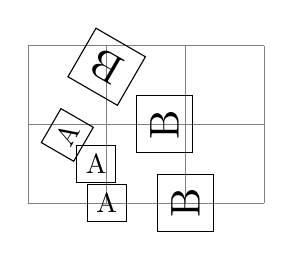
\begin{tikzpicture}[every node/.style={draw}]
  \draw[help lines](0,0) grid (3,2);
  \draw            (1,0) node{A}
                   (2,0) node[rotate=90,scale=1.5] {B};
  \draw[rotate=30] (1,0) node{A}
                   (2,0) node[rotate=90,scale=1.5] {B};
  \draw[rotate=60] (1,0) node[transform shape] {A}
                   (2,0) node[transform shape,rotate=90,scale=1.5] {B};
\end{tikzpicture}
\end{codeexample}
        %
\end{enumerate}

Even though \tikzname\ currently does not allow you to configure so-called
\emph{nonlinear transformations,} see
Section~\ref{section-nonlinear-transformations}, there is an option that
influences how nodes are transformed when nonlinear transformations are in
force:
%
\begin{key}{/tikz/transform shape nonlinear=\opt{\meta{true or false}}  (initially false)}
    When set to true, \tikzname\ will try to apply any current nonlinear
    transformation also to nodes. Typically, for the text in nodes this is not
    possible in general, in such cases a linear approximation of the nonlinear
    transformation is used. For more details, see
    Section~\ref{section-nonlinear-transformations}.
    %
\makeatletter
\begin{codeexample}[
    preamble={\usepgfmodule{nonlineartransformations}\usetikzlibrary{curvilinear}},
    pre={\makeatletter},
]
\begin{tikzpicture}
   % Install a nonlinear transformation:
   \pgfsetcurvilinearbeziercurve
      {\pgfpoint{0mm}{20mm}}
      {\pgfpoint{10mm}{20mm}}
      {\pgfpoint{10mm}{10mm}}
      {\pgfpoint{20mm}{10mm}}
   \pgftransformnonlinear{\pgfpointcurvilinearbezierorthogonal\pgf@x\pgf@y}%

   % Draw something:
   \draw [help lines] (0,-30pt) grid [step=10pt] (80pt,30pt);

   \foreach \x in {0,20,...,80}
     \node [fill=red!20]  at (\x pt, -20pt) {\x};

   \foreach \x in {0,20,...,80}
     \node [fill=blue!20, transform shape nonlinear] at (\x pt, 20pt) {\x};
\end{tikzpicture}
\end{codeexample}
    %
\end{key}


\subsection{Placing Nodes on a Line or Curve Explicitly}
\label{section-nodes-placing-1}

Until now, we always placed nodes on a coordinate that is mentioned in the path.
Often, however, we wish to place nodes on ``the middle'' of a line and we do
not wish to compute these coordinates ``by hand''. To facilitate such
placements, \tikzname\ allows you to specify that a certain node should be
somewhere ``on'' a line. There are two ways of specifying this: Either
explicitly by using the |pos| option or implicitly by placing the node
``inside'' a path operation. These two ways are described in the following.

    \label{section-pos-option}

\begin{key}{/tikz/pos=\meta{fraction}}
    When this option is given, the node is not anchored on the last coordinate.
    Rather, it is anchored on some point on the line from the previous
    coordinate to the current point. The \meta{fraction} dictates how ``far''
    on the line the point should be. A \meta{fraction} of 0 is the previous
    coordinate, 1 is the current one, everything else is in between. In
    particular, 0.5 is the middle.

    Now, what is ``the previous line''? This depends on the previous path
    construction operation.

    In the simplest case, the previous path operation was a ``line-to''
    operation, that is, a |--|\meta{coordinate} operation:
    %
\begin{codeexample}[]
\tikz \draw (0,0) -- (3,1)
    node[pos=0]{0} node[pos=0.5]{1/2} node[pos=0.9]{9/10};
\end{codeexample}

    For the |arc| operation, the position is simply the corresponding position
    on the arc:
    %
\begin{codeexample}[]
\tikz {
  \draw [help lines] (0,0) grid (3,2);
  \draw (2,0) arc [x radius=1, y radius=2, start angle=0, end angle=180]
              node foreach \t in {0,0.125,...,1} [pos=\t,auto] {\t};
}
\end{codeexample}

    The next case is the curve-to operation (the |..| operation). In this case,
    the ``middle'' of the curve, that is, the position |0.5| is not necessarily
    the point at the exact half distance on the line. Rather, it is some point
    at ``time'' 0.5 of a point traveling from the start of the curve, where it
    is at time 0, to the end of the curve, which it reaches at time 0.5. The
    ``speed'' of the point depends on the length of the support vectors (the
    vectors that connect the start and end points to the control points). The
    exact math is a bit complicated (depending on your point of view, of
    course); you may wish to consult a good book on computer graphics and
    Bézier curves if you are intrigued.
    %
\begin{codeexample}[]
\tikz \draw (0,0) .. controls +(right:3.5cm) and +(right:3.5cm) .. (0,3)
  node foreach \p in {0,0.125,...,1} [pos=\p]{\p};
\end{codeexample}

    Another interesting case are the horizontal/vertical line-to operations
    \verb!|-! and \verb!-|!. For them, the position (or time) |0.5| is exactly
    the corner point.
    %
\begin{codeexample}[]
\tikz \draw (0,0) |- (3,1)
  node[pos=0]{0} node[pos=0.5]{1/2} node[pos=0.9]{9/10};
\end{codeexample}

\begin{codeexample}[]
\tikz \draw (0,0) -| (3,1)
  node[pos=0]{0} node[pos=0.5]{1/2} node[pos=0.9]{9/10};
\end{codeexample}

    For all other path construction operations, \emph{the position placement
    does not work}, currently.
\end{key}

\begin{key}{/tikz/auto=\opt{\meta{direction}} (default \normalfont is scope's setting)}
    This option causes an anchor position to be calculated automatically
    according to the following rule. Consider a line between two points. If the
    \meta{direction} is |left|, then the anchor is chosen such that the node is
    to the left of this line. If the \meta{direction} is |right|, then the node
    is to the right of this line. Leaving out \meta{direction} causes automatic
    placement to be enabled with the last value of |left| or |right| used. A
    \meta{direction} of |false| disables automatic placement. This happens also
    whenever an anchor is given explicitly by the |anchor| option or by one of
    the |above|, |below|, etc.\ options.

    This option only has an effect for nodes that are placed on lines or
    curves.
    %
\begin{codeexample}[]
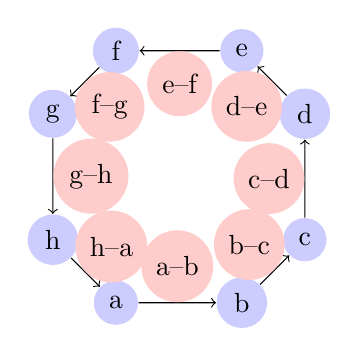
\begin{tikzpicture}
  [scale=.8,auto=left,every node/.style={circle,fill=blue!20}]
  \node (a) at (-1,-2) {a};
  \node (b) at ( 1,-2) {b};
  \node (c) at ( 2,-1) {c};
  \node (d) at ( 2, 1) {d};
  \node (e) at ( 1, 2) {e};
  \node (f) at (-1, 2) {f};
  \node (g) at (-2, 1) {g};
  \node (h) at (-2,-1) {h};

  \foreach \from/\to in {a/b,b/c,c/d,d/e,e/f,f/g,g/h,h/a}
    \draw [->] (\from) -- (\to)
               node[midway,fill=red!20] {\from--\to};
\end{tikzpicture}
\end{codeexample}
    %
\end{key}

\begin{key}{/tikz/swap}
    This option exchanges the roles of |left| and |right| in automatic
    placement. That is, if |left| is the current |auto| placement, |right| is
    set instead and the other way round.
    %
\begin{codeexample}[preamble={\usetikzlibrary{automata}}]
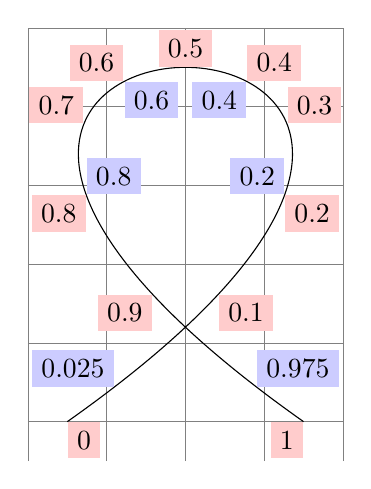
\begin{tikzpicture}[auto]
  \draw[help lines,use as bounding box] (0,-.5) grid (4,5);

  \draw (0.5,0) .. controls (9,6) and (-5,6) .. (3.5,0)
    node foreach \pos in {0,0.1,0.2,0.3,0.4,0.5,0.6,0.7,0.8,0.9,1}
         [pos=\pos,swap,fill=red!20] {\pos}
    node foreach \pos in {0.025,0.2,0.4,0.6,0.8,0.975}
         [pos=\pos,fill=blue!20] {\pos};
\end{tikzpicture}
\end{codeexample}
    %
\begin{codeexample}[preamble={\usetikzlibrary{automata}}]
\begin{tikzpicture}[shorten >=1pt,node distance=2cm,auto]
  \draw[help lines] (0,0) grid (3,2);

  \node[state] (q_0)                      {$q_0$};
  \node[state] (q_1) [above right of=q_0] {$q_1$};
  \node[state] (q_2) [below right of=q_0] {$q_2$};
  \node[state] (q_3) [below right of=q_1] {$q_3$};

  \path[->] (q_0) edge              node        {0} (q_1)
                  edge              node [swap] {1} (q_2)
            (q_1) edge              node        {1} (q_3)
                  edge [loop above] node        {0} ()
            (q_2) edge              node [swap] {0} (q_3)
                  edge [loop below] node        {1} ();
\end{tikzpicture}
\end{codeexample}
    %
\end{key}

\begin{key}{/tikz/'}
    This is a very short alias for |swap|.
\end{key}

\begin{key}{/tikz/sloped}
    This option causes the node to be rotated such that a horizontal line
    becomes a tangent to the curve. The rotation is normally done in such a way
    that text is never ``upside down''. To get upside-down text, use can use
    |[rotate=180]| or |[allow upside down]|, see below.
    %
\begin{codeexample}[]
\tikz \draw (0,0) .. controls +(up:2cm) and +(left:2cm) .. (1,3)
    node foreach \p in {0,0.25,...,1} [sloped,above,pos=\p]{\p};
\end{codeexample}
    %
\begin{codeexample}[]
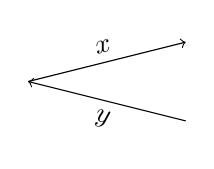
\begin{tikzpicture}[->]
  \draw (0,0)   -- (2,0.5) node[midway,sloped,above] {$x$};
  \draw (2,-.5) -- (0,0)   node[midway,sloped,below] {$y$};
\end{tikzpicture}
\end{codeexample}
    %
\end{key}


\begin{key}{/tikz/allow upside down=\meta{boolean} (default true, initially false)}
    If set to |true|, \tikzname\ will not ``righten'' upside down text.
    %
\begin{codeexample}[]
\tikz [allow upside down]
  \draw (0,0) .. controls +(up:2cm) and +(left:2cm) .. (1,3)
    node foreach \p in {0,0.25,...,1} [sloped,above,pos=\p]{\p};
\end{codeexample}
    %
\begin{codeexample}[]
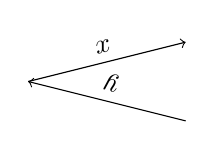
\begin{tikzpicture}[->,allow upside down]
  \draw (0,0)   -- (2,0.5) node[midway,sloped,above] {$x$};
  \draw (2,-.5) -- (0,0)   node[midway,sloped,below] {$y$};
\end{tikzpicture}
\end{codeexample}
    %
\end{key}

There exist styles for specifying positions a bit less ``technically'':

\begin{stylekey}{/tikz/midway}
    This has the same effect as |pos=0.5|.
    %
\begin{codeexample}[]
\tikz \draw (0,0) .. controls +(up:2cm) and +(left:3cm) .. (1,5)
       node[at end]          {\texttt{at end}}
       node[very near end]   {\texttt{very near end}}
       node[near end]        {\texttt{near end}}
       node[midway]          {\texttt{midway}}
       node[near start]      {\texttt{near start}}
       node[very near start] {\texttt{very near start}}
       node[at start]        {\texttt{at start}};
\end{codeexample}
    %
\end{stylekey}

\begin{stylekey}{/tikz/near start}
    Set to |pos=0.25|.
\end{stylekey}

\begin{stylekey}{/tikz/near end}
    Set to |pos=0.75|.
\end{stylekey}

\begin{stylekey}{/tikz/very near start}
    Set to |pos=0.125|.
\end{stylekey}

\begin{stylekey}{/tikz/very near end}
    Set to |pos=0.875|.
\end{stylekey}

\begin{stylekey}{/tikz/at start}
    Set to |pos=0|.
\end{stylekey}

\begin{stylekey}{/tikz/at end}
    Set to |pos=1|.
\end{stylekey}


\subsection{Placing Nodes on a Line or Curve Implicitly}
\label{section-nodes-placing-2}

When you wish to place a node on the line |(0,0) -- (1,1)|, it is natural to
specify the node not following the |(1,1)|, but ``somewhere in the middle''.
This is, indeed, possible and you can write |(0,0) -- node{a} (1,1)| to place a
node midway between |(0,0)| and |(1,1)|.

What happens is the following: The syntax of the line-to path operation is
actually |--| \opt{|node|\meta{node specification}}\meta{coordinate}. (It is
even possible to give multiple nodes in this way.) When the optional |node| is
encountered, that is, when the |--| is directly followed by |node|, then the
specification(s) are read and ``stored away''. Then, after the
\meta{coordinate} has finally been reached, they are inserted again, but with
the |pos| option set.

There are two things to note about this: When a node specification is
``stored'', its catcodes become fixed. This means that you cannot use overly
complicated verbatim text in them. If you really need, say, a verbatim text,
you will have to put it in a normal node following the coordinate and add the
|pos| option.

Second, which |pos| is chosen for the node? The position is inherited from the
surrounding scope. However, this holds only for nodes specified in this
implicit way. Thus, if you add the option |[near end]| to a scope, this does
not mean that \emph{all} nodes given in this scope will be put on near the end
of lines. Only the nodes for which an implicit |pos| is added will be placed
near the end. Typically, this is what you want. Here are some examples that
should make this clearer:
%
\begin{codeexample}[]
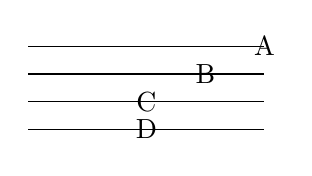
\begin{tikzpicture}[near end]
  \draw (0cm,4em) -- (3cm,4em) node{A};
  \draw (0cm,3em) --           node{B}          (3cm,3em);
  \draw (0cm,2em) --           node[midway] {C} (3cm,2em);
  \draw (0cm,1em) -- (3cm,1em) node[midway] {D} ;
\end{tikzpicture}
\end{codeexample}

Like the line-to operation, the curve-to operation |..| also allows you to
specify nodes ``inside'' the operation. After both the first |..| and also
after the second |..| you can place node specifications. Like for the |--|
operation, these will be collected and then reinserted after the operation with
the |pos| option set.


\subsection{The Label and Pin Options}

\subsubsection{Overview}

In addition to the |node| path operation, the two options |label| and |pin| can
be used to ``add a node next to another node''. As an example, suppose we want
to draw a graph in which the nodes are small circles:
%
\begin{codeexample}[preamble={\usetikzlibrary{positioning}}]
\tikz [circle] {
  \node [draw] (s) {};
  \node [draw] (a) [right=of s] {} edge (s);
  \node [draw] (b) [right=of a] {} edge (a);
  \node [draw] (t) [right=of b] {} edge (b);
}
\end{codeexample}

Now, in the above example, suppose we wish to indicate that the first node is
the start node and the last node is the target node. We could write
|\node (s) {$s$};|, but this would enlarge the first node. Rather, we want the
``$s$'' to be placed next to the node. For this, we need to create
\emph{another} node, but next to the existing node. The |label| and |pin|
option allow us to do exactly this without having to use the cumbersome |node|
syntax:
%
\begin{codeexample}[preamble={\usetikzlibrary{positioning}}]
\tikz [circle] {
  \node [draw] (s) [label=$s$]  {};
  \node [draw] (a) [right=of s] {} edge (s);
  \node [draw] (b) [right=of a] {} edge (a);
  \node [draw] (t) [right=of b, label=$t$] {} edge (b);
}
\end{codeexample}


\subsubsection{The Label Option}

\begin{key}{/tikz/label=\opt{|[|\meta{options}|]|\meta{angle}|:|}\meta{text}}
        \label{label-option}%
    When this option is given to a |node| operation, it causes \emph{another}
    node to be added to the path after the current node has been finished. This
    extra node will have the text \meta{text}. It is placed, in principle, in
    the direction \meta{angle} relative to the main node, but the exact rules
    are a bit complex. Suppose the |node| currently under construction is
    called |main node| and let us call the label node |label node|. Then the
    following happens:
    %
    \begin{enumerate}
        \item The \meta{angle} is used to determine a position on the border of
            the |main node|. If the \meta{angle} is missing, the value of the
            following key is used instead:
            %
            \begin{key}{/tikz/label position=\meta{angle} (initially above)}
                Sets the default position for labels.
            \end{key}
            %
            The \meta{angle} determines the position on the border of the shape
            in two different ways. Normally, the border position is given by
            |main node.|\meta{angle}. This means that the \meta{angle} can
            either be a number like |0| or |-340|, but it can also be an anchor
            like |north|. Additionally, the special angles |above|, |below|,
            |left|, |right|, |above left|, and so on are automatically replaced
            by the corresponding angles |90|, |270|, |180|, |0|, |135|, and so
            on.

            A special case arises when the following key is set:
            %
            \begin{key}{/tikz/absolute=\meta{true or false} (default true)}
                When this key is set, the \meta{angle} is interpreted
                differently: We still use a point on the border of the
                |main node|, but the angle is measured ``absolutely'', that is,
                an angle of |0| refers to the point on the border that lies on
                a straight line from the |main node|'s center to the right
                (relative to the paper, not relative to the local coordinate
                system of either the node or the scope).

                The difference can be seen in the following example:
                %
\begin{codeexample}[]
\tikz [rotate=-80,every label/.style={draw,red}]
  \node [transform shape,rectangle,draw,label=right:label] {main node};
\end{codeexample}
                %
\begin{codeexample}[]
\tikz [rotate=-80,every label/.style={draw,red},absolute]
  \node [transform shape,rectangle,draw,label=right:label] {main node};
\end{codeexample}
            \end{key}
        \item Then, an anchor point for the |label node| is computed. It is
            determined in such a way that the |label node| will ``face away''
            from the border of the |main node|. The anchor that is chosen
            depends on the position of the border point that is chosen and its
            position relative to the center of the |main node| and on whether
            the |transform shape| option is set. In detail, when the computed
            border point is at $0^\circ$, the anchor |west| will be used.
            Similarly, when the border point is at $90^\circ$, the anchor
            |south| will be used, and so on for $180^\circ$ and $270^\circ$.

            For angles between these ``major'' angles, like $30^\circ$ or
            $110^\circ$, combined anchors, like |south west| for $30^\circ$ or
            |south east| for $110^\circ$, are used. However, for angles close
            to the major angles, (differing by up to $2^\circ$ from the major
            angle), the anchor for the major angle is used. Thus, a label at a
            border point for $2^\circ$ will have the anchor |west|, while a
            label for $3^\circ$ will have the anchor |south west|, resulting in
            a ``jump'' of the anchor. You can set the anchor ``by hand'' using
            the |anchor| key or indirect keys like |left|.
            %
\begin{codeexample}[]
\tikz
  \node [circle, draw,
         label=default,
         label=60:$60^\circ$,
         label=below:$-90^\circ$,
         label=3:$3^\circ$,
         label=2:$2^\circ$,
         label={[below]180:$180^\circ$},
         label={[centered]135:$135^\circ$}] {my circle};
\end{codeexample}
        \item One \meta{angle} is special: If you set the \meta{angle} to
            |center|, then the label will be placed on the center of the main
            node. This is mainly useful for adding a label text to an existing
            node, especially if it has been rotated.
            %
\begin{codeexample}[]
\tikz \node [transform shape,rotate=90,
             rectangle,draw,label={[red]center:R}] {main node};
\end{codeexample}
    \end{enumerate}

    You can pass \meta{options} to the node |label node|. For this, you provide
    the options in square brackets before the \meta{angle}. If you do so, you
    need to add braces around the whole argument of the |label| option and this
    is also the case if you have brackets or commas or semicolons or anything
    special in the \meta{text}.
    %
\begin{codeexample}[]
\tikz \node [circle,draw,label={[red]above:X}] {my circle};
\end{codeexample}

\begin{codeexample}[]
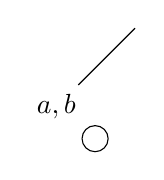
\begin{tikzpicture}
  \node [circle,draw,label={[name=label node]above left:$a,b$}] {};
  \draw (label node) -- +(1,1);
\end{tikzpicture}
\end{codeexample}

    If you provide multiple |label| options, then multiple extra label nodes
    are added in the order they are given.

    The following styles influence how labels are drawn:
    %
    \begin{key}{/tikz/label distance=\meta{distance} (initially 0pt)}
        The \meta{distance} is additionally inserted between the main node and
        the label node.
        %
\begin{codeexample}[]
\tikz[label distance=5mm]
  \node [circle,draw,label=right:X,
                     label=above right:Y,
                     label=above:Z]       {my circle};
\end{codeexample}
    \end{key}
    %
    \begin{stylekey}{/tikz/every label (initially \normalfont empty)}
        This style is used in every node created by the |label| option. The
        default is |draw=none,fill=none|.
    \end{stylekey}
\end{key}

See Section~\ref{section-label-quotes} for an easier syntax for specifying
nodes.


\subsubsection{The Pin Option}

\begin{key}{/tikz/pin=\opt{|[|\meta{options}|]|}\meta{angle}|:|\meta{text}}
    This option is quite similar to the |label| option, but there is one
    difference: In addition to adding an extra node to the picture, it also
    adds an edge from this node to the main node. This causes the node to look
    like a pin that has been added to the main node:
    %
\begin{codeexample}[]
\tikz \node [circle,fill=blue!50,minimum size=1cm,pin=60:$q_0$] {};
\end{codeexample}

    The meaning of the \meta{options} and the \meta{angle} and the \meta{text}
    is exactly the same as for the |node| option. Only, the options and styles
    the influence the way pins look are different:
    %
    \begin{key}{/tikz/pin distance=\meta{distance} (initially 3ex)}
        This \meta{distance} is used instead of the |label distance| for the
        distance between the main node and the label node.
        %
\begin{codeexample}[]
\tikz[pin distance=1cm]
  \node [circle,draw,pin=right:X,
                     pin=above right:Y,
                     pin=above:Z]       {my circle};
\end{codeexample}
        %
    \end{key}

    \begin{stylekey}{/tikz/every pin (initially {draw=none,fill=none})}
        This style is used in every node created by the |pin| option.
    \end{stylekey}

    \begin{key}{/tikz/pin position=\meta{angle} (initially above)}
        The default pin position. Works like |label position|.
    \end{key}

    \begin{stylekey}{/tikz/every pin edge (initially help lines)}
        This style is used in every edge created by the |pin| options.
        %
\begin{codeexample}[preamble={\usetikzlibrary{decorations.pathmorphing}}]
\tikz [pin distance=15mm,
       every pin edge/.style={<-,shorten <=1pt,decorate,
                              decoration={snake,pre length=4pt}}]
  \node [circle,draw,pin=right:X,
                     pin=above right:Y,
                     pin=above:Z]       {my circle};
\end{codeexample}
    \end{stylekey}

    \begin{key}{/tikz/pin edge=\meta{options} (initially \normalfont empty)}
        This option can be used to set the options that are to be used in the
        edge created by the |pin| option.
        %
\begin{codeexample}[]
\tikz[pin distance=10mm]
  \node [circle,draw,pin={[pin edge={blue,thick}]right:X},
                     pin=above:Z]       {my circle};
\end{codeexample}
        %
\begin{codeexample}[]
\tikz [every pin edge/.style={},
       initial/.style={pin={[pin distance=5mm,
                             pin edge={<-,shorten <=1pt}]left:start}}]
  \node [circle,draw,initial] {my circle};
\end{codeexample}
    \end{key}
\end{key}


\subsubsection{The Quotes Syntax}
\label{section-label-quotes}

The |label| and |pin| options provide a syntax for creating nodes next to
existing nodes, but this syntax is often a bit too verbose. By including the
following library, you get access to an even more concise syntax:

\begin{tikzlibrary}{quotes}
    Enables the quotes syntax for labels, pins, edge nodes, and pic texts.
\end{tikzlibrary}

Let us start with the basics of what this library does: Once loaded, inside the
options of a |node| command, instead of the usual \meta{key}|=|\meta{value}
pairs, you may also provide strings of the following form (the actual syntax is
slightly more general, see the detailed descriptions later on):
%
\begin{quote}
    |"|\meta{text}|"|\opt{\meta{options}}
\end{quote}
%
The \meta{options} must be surrounded in curly braces when they contain a
comma, otherwise the curly braces are optional. The \meta{options} may be
preceded by an optional space.

When a \meta{string} of the above form is encountered inside the options of a
|node|, then it is internally transformed to
%
% (the double vertical bar after = is needed to avoid the two opening brackets
%  being typeset in italics)
\begin{quote}
    |label=||{[|\meta{options}|]|\meta{text}|}|
\end{quote}

Let us have a look at an example:
%
\begin{codeexample}[preamble={\usetikzlibrary{quotes}}]
\tikz \node ["my label" red, draw] {my node};
\end{codeexample}
%
The above has the same effect as the following:
%
\begin{codeexample}[]
\tikz \node [label={[red]my label}, draw] {my node};
\end{codeexample}

Here are further examples, one where no \meta{options} are added to the
|label|, one where a position is specified, and examples with more complicated
options in curly braces:
%
\begin{codeexample}[preamble={\usetikzlibrary{quotes}}]
\begin{tikzpicture}
  \matrix [row sep=5mm] {
    \node [draw, "label"]                  {A}; \\
    \node [draw, "label" left]             {B}; \\
    \node [draw, "label" centered]         {C}; \\
    \node [draw, "label" color=red]        {D}; \\
    \node [draw, "label" {red,draw,thick}] {E}; \\
  };
\end{tikzpicture}
\end{codeexample}

Let us now have a more detailed look at what commands this library
provides:

\begin{key}{/tikz/quotes mean label}
    When this option is used (which is the default when this library is
    loaded), then, as described above, inside the options of a node a special
    syntax check is done.

    \medskip
    \noindent\textbf{The syntax.}
    For each string in the list of options it is tested whether it starts with
    a quotation mark (note that this will never happen for normal keys since
    the normal keys of \tikzname\ do not start with quotation marks). When this
    happens, the \meta{string} should not be a key--value pair, but, rather,
    must have the form:
    %
    \begin{quote}
        |"|\meta{text}|"|\opt{|'|}\opt{\meta{options}}
    \end{quote}

    (We will discuss the optional apostrophe in a moment. It is not really
    important for the current option, but only for edge labels, which are
    discussed later).

    \medskip
    \noindent\textbf{Transformation to a label option.}
    When a \meta{string} has the above form, it is treated (almost) as if you
    had written
    %
    \begin{quote}
        |label={[|\meta{options}|]|\meta{text}|}|
    \end{quote}
    %
    instead. The ``almost'' refers to the following additional feature: In
    reality, before the \meta{options} are executed inside the |label| command,
    the direction keys |above|, |left|, |below right| and so on are redefined
    so that |above| is a shorthand for |label position=90| and similarly for
    the other keys. The net effect is that in order to specify the position of
    the \meta{text} relative to the main node you can just put something like
    |left| or |above right| inside the \meta{options}:
    %
\begin{codeexample}[preamble={\usetikzlibrary{quotes}}]
\tikz
  \node ["$90^\circ$" above, "$180^\circ$" left, circle, draw] {circle};
\end{codeexample}

    Alternatively, you can also use \meta{direction}|:|\meta{actual text} as
    your \meta{text}. This works since the |label| command allows you to
    specify a direction at the beginning when it is separated by a colon:
    %
\begin{codeexample}[preamble={\usetikzlibrary{quotes}}]
\tikz
  \node ["90:$90^\circ$", "left:$180^\circ$", circle, draw] {circle};
\end{codeexample}
    %
    Arguably, placing |above| or |left| behind the \meta{text} seems more
    natural than having it inside the \meta{text}.

    In addition to the above, before the \meta{options} are executed, the
    following style is also executed:
    %
    \begin{stylekey}{/tikz/every label quotes}
\begin{codeexample}[preamble={\usetikzlibrary{quotes}}]
\tikz [every label quotes/.style=red]
  \node ["90:$90^\circ$", "left:$180^\circ$", circle, draw] {circle};
\end{codeexample}
    \end{stylekey}

    \medskip
    \noindent\textbf{Handling commas and colons inside the text.}
    The \meta{text} may not contain a comma, unless it is inside curly braces.
    The reason is that the key handler separates the total options of a |node|
    along the commas it finds. So, in order to have text containing a comma,
    just add curly braces around either the comma or just around the whole
    \meta{text}:
    %
\begin{codeexample}[preamble={\usetikzlibrary{quotes}}]
\tikz \node ["{yes, we can}", draw] {foo};
\end{codeexample}
    %
    The same is true for a colon, only in this case you may need to surround
    specifically the colon by curly braces to stop the |label| option from
    interpreting everything before the colon as a direction:
    %
\begin{codeexample}[preamble={\usetikzlibrary{quotes}}]
\tikz \node ["yes{:} we can", draw] {foo};
\end{codeexample}

    \medskip
    \noindent\textbf{The optional apostrophe.}
    Following the closing quotation marks in a \meta{string} there may (but
    need not) be a single quotation mark (an apostrophe), possibly surrounded
    by whitespaces. If it is present, it is simply added to the \meta{options}
    as another option (and, indeed, a single apostrophe is a legal option in
    \tikzname, it is a shorthand for |swap|):

    \begin{tabular}{ll}
        String         & has the same effect as \\\hline
        |"foo"'|       & |"foo" {'}| \\
        |"foo"' red|   & |"foo" {',red}| \\
        |"foo"'{red}|  & |"foo" {',red}| \\
        |"foo"{',red}| & |"foo" {',red}| \\
        |"foo"{red,'}| & |"foo" {red,'}| \\
        |"foo"{'red}|  & |"foo" {'red}| (illegal; there is no key |'red|)\\
        |"foo" red'|   & |"foo" {red'}| (illegal; there is no key |red'|)\\
    \end{tabular}
\end{key}

\begin{key}{/tikz/quotes mean pin}
    This option has exactly the same effect as |quotes mean label|, only
    instead of transforming quoted text to the |label| option, they get
    transformed to the |pin| option:
    %
\begin{codeexample}[preamble={\usetikzlibrary{quotes}}]
\tikz [quotes mean pin]
  \node ["$90^\circ$" above, "$180^\circ$" left, circle, draw] {circle};
\end{codeexample}
    %
    Instead of |every label quotes|, the following style is executed
    with each such pin:
    %
    \begin{stylekey}{/tikz/every pin quotes}
    \end{stylekey}
\end{key}

If instead of |label|s or |pin|s you would like quoted strings to be
interpreted in a different manner, you can also define your own handlers:

\begin{key}{/tikz/node quotes mean=\meta{replacement}}
    This key allows you to define your own handler for quotes options. Inside
    the options of a |node|, whenever a key--value pair with the syntax
    %
    \begin{quote}
        |"|\meta{text}|"|\opt{|'|}\opt{\meta{options}}
    \end{quote}
    %
    is encountered, the following happens: The above string gets replaced by
    \meta{replacement} where inside the \meta{replacement} the parameter |#1|
    is \meta{text} and |#2| is \meta{options}. If the apostrophe is present
    (see also the discussion of |quotes mean label|), the \meta{options} start
    with |',|.

    The \meta{replacement} is then parsed normally as options (using
    |\pgfkeys|).

    Here is an example, where the quotes are used to define labels that are
    automatically named according to the |text|:
    %
\begin{codeexample}[preamble={\usetikzlibrary{quotes}}]
\tikzset{node quotes mean={label={[#2,name={#1}]#1}}}

\tikz {
  \node ["1", "2" label position=left, circle, draw] {circle};
  \draw (1) -- (2);
}
\end{codeexample}
    %
\end{key}

Some further options provided by the |quotes| library concern labels next to
edges rather than nodes and they are described in
Section~\ref{section-edge-quotes}.


\subsection{Connecting Nodes: Using Nodes as Coordinates}
\label{section-nodes-connecting}

Once you have defined a node and given it a name, you can use this name to
reference it. This can be done in two ways, see also
Section~\ref{section-node-coordinates}. Suppose you have said
|\path(0,0) node(x) {Hello World!};| in order to define a node named |x|.
%
\begin{enumerate}
    \item Once the node |x| has been defined, you can use |(x.|\meta{anchor}|)|
        wherever you would normally use a normal coordinate. This will yield
        the position at which the given \meta{anchor} is in the picture. Note
        that transformations do not apply to this coordinate, that is,
        |(x.north)| will be the northern anchor of |x| even if you have said
        |scale=3| or |xshift=4cm|. This is usually what you would expect.
    \item You can also just use |(x)| as a coordinate. In most cases, this
        gives the same coordinate as |(x.center)|. Indeed, if the |shape| of
        |x| is |coordinate|, then |(x)| and |(x.center)| have exactly the same
        effect.

        However, for most other shapes, some path construction operations like
        |--| try to be ``clever'' when they are asked to draw a line from such
        a coordinate or to such a coordinate. When you say |(x)--(1,1)|, the
        |--| path operation will not draw a line from the center of |x|, but
        \emph{from the border} of |x| in the direction going towards |(1,1)|.
        Likewise, |(1,1)--(x)| will also have the line end on the border in the
        direction coming from |(1,1)|.

        If the specified coordinate is almost identical to the node center, for
        example |(x)--(0,0)|, no line will be drawn and a warning message will
        be printed.

        In addition to |--|, the curve-to path operation |..| and the path
        operations \verb!-|! and \verb!|-! will also handle nodes without
        anchors correctly. Here is an example, see also
        Section~\ref{section-node-coordinates}:
        %
\begin{codeexample}[]
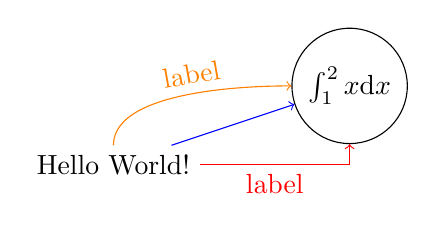
\begin{tikzpicture}
  \path (0,0) node             (x) {Hello World!}
        (3,1) node[circle,draw](y) {$\int_1^2 x \mathrm d x$};

  \draw[->,blue]   (x) -- (y);
  \draw[->,red]    (x) -| node[near start,below] {label} (y);
  \draw[->,orange] (x) .. controls +(up:1cm) and +(left:1cm) .. node[above,sloped] {label} (y);
\end{tikzpicture}
\end{codeexample}
        %
\end{enumerate}


\subsection{Connecting Nodes: Using the Edge Operation}
\label{section-nodes-edges}

\subsubsection{Basic Syntax of the Edge Operation}

The |edge| operation works like a |to| operation that is added after the main
path has been drawn, much like a node is added after the main path has been
drawn. This allows each |edge| to have a different appearance. As the |node|
operation, an |edge| temporarily suspends the construction of the current path
and a new path $p$ is constructed. This new path $p$ will be drawn after the
main path has been drawn. Note that $p$ can be totally different from the main
path with respect to its options. Also note that if there are several |edge|
and/or |node| operations in the main path, each creates its own path(s) and
they are drawn in the order that they are encountered on the main path.

\begin{pathoperation}{edge}{\opt{|[|\meta{options}|]|} \opt{\meta{nodes}} |(|\meta{coordinate}|)|}
    The effect of the |edge| operation is that after the main path the
    following path is added to the picture:
    %
    \begin{quote}
        |\path[every edge,|\meta{options}|] (\tikztostart) |\meta{path}|;|
    \end{quote}
    %
    Here, \meta{path} is the |to path|. Note that, unlike the path added by the
    |to| operation, the |(\tikztostart)| is added before the \meta{path} (which
    is unnecessary for the |to| operation, since this coordinate is already
    part of the main path).

    The |\tikztostart| is the last coordinate on the path just before the
    |edge| operation, just as for the |node| or |to| operations. However, there
    is one exception to this rule: If the |edge| operation is directly preceded
    by a |node| operation, then this just-declared node is the start coordinate
    (and not, as would normally be the case, the coordinate where this
    just-declared node is placed -- a small, but subtle difference). In this
    regard, |edge| differs from both |node| and |to|.

    If there are several |edge| operations in a row, the start coordinate is
    the same for all of them as their target coordinates are not, after all,
    part of the main path. The start coordinate is, thus, the coordinate
    preceding the first |edge| operation. This is similar to nodes insofar as
    the |edge| operation does not modify the current path at all. In
    particular, it does not change the last coordinate visited, see the
    following example:
    %
\begin{codeexample}[]
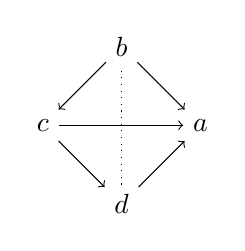
\begin{tikzpicture}
  \node (a) at   (0:1) {$a$};
  \node (b) at  (90:1) {$b$} edge [->]     (a);
  \node (c) at (180:1) {$c$} edge [->]     (a)
                             edge [<-]     (b);
  \node (d) at (270:1) {$d$} edge [->]     (a)
                             edge [dotted] (b)
                             edge [<-]     (c);
\end{tikzpicture}
\end{codeexample}

    A different way of specifying the above graph using the |edge| operation is
    the following:
    %
\begin{codeexample}[]
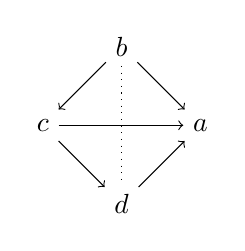
\begin{tikzpicture}
  \node foreach \name/\angle in {a/0,b/90,c/180,d/270}
        (\name) at (\angle:1) {$\name$};

  \path[->] (b) edge (a)
                edge (c)
                edge [-,dotted] (d)
            (c) edge (a)
                edge (d)
            (d) edge (a);
\end{tikzpicture}
\end{codeexample}

    As can be seen, the path of the |edge| operation inherits the options from
    the main path, but you can locally overrule them.
    %
\begin{codeexample}[]
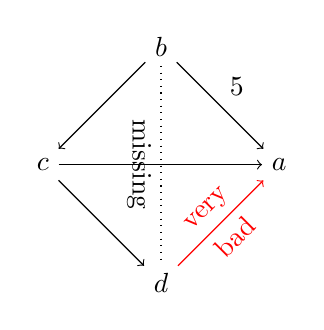
\begin{tikzpicture}
  \node foreach \name/\angle in {a/0,b/90,c/180,d/270}
        (\name) at (\angle:1.5) {$\name$};

  \path[->] (b) edge            node[above right]  {$5$}     (a)
                edge                                         (c)
                edge [-,dotted] node[below,sloped] {missing} (d)
            (c) edge                                         (a)
                edge                                         (d)
            (d) edge [red]      node[above,sloped] {very}
                                node[below,sloped] {bad}     (a);
\end{tikzpicture}
\end{codeexample}

    Instead of |every to|, the style |every edge| is installed at the beginning
    of the main path.
    %
    \begin{stylekey}{/tikz/every edge (initially draw)}
        Executed for each |edge|.
        %
\begin{codeexample}[]
\begin{tikzpicture}[every edge/.style={draw,dashed}]
  \path (0,0) edge (3,2);
\end{tikzpicture}
\end{codeexample}
    \end{stylekey}
\end{pathoperation}


\subsubsection{Nodes on Edges: Quotes Syntax}
\label{section-edge-quotes}

The standard way of specifying nodes that are placed ``on'' an edge (or on a
to-path; all of the following is also true for to--paths) is to put node
specifications after the |edge| keyword, but before the target coordinate.
Another way is to use the |edge node| option and its friends. Yet another way
is to use the quotes syntax.

The syntax is essentially the same as for labels added to nodes as described in
Section~\ref{section-label-quotes} and you also need to load the |quotes|
library.

In detail, when the |quotes| library is loaded, each time a key--value pair in
a list of options passed to an |edge| or a |to| path command starts with |"|,
the key--value pair must actually be a string of the following form:
%
\begin{quote}
    |"|\meta{text}|"|\opt{|'|}\opt{\meta{options}}
\end{quote}
%
This string is transformed into the following:
%
\begin{quote}
    |edge node=node [every edge quotes,|\meta{options}|]{|\meta{text}|}|
\end{quote}
%
As described in Section~\ref{section-label-quotes}, the apostrophe becomes part
of the \meta{options}, when present.

The following style is important for the placement of the labels:

\begin{stylekey}{/tikz/every edge quotes (initially auto)}
    This style is |auto| by default, which causes labels specified using the
    quotes-syntax to be placed next to the edges. Unless the setting of |auto|
    has been changed, they will be placed to the left.
    %
\begin{codeexample}[preamble={\usetikzlibrary{quotes}}]
\tikz \draw (0,0) edge ["left", ->] (2,0);
\end{codeexample}

    In order to place all labels to the right by default, change this style to
    |auto=right|:
    %
\begin{codeexample}[preamble={\usetikzlibrary{quotes}}]
\tikz [every edge quotes/.style={auto=right}]
  \draw (0,0) edge ["right", ->] (2,0);
\end{codeexample}

    To place all nodes ``on'' the edge, just make this style empty (and,
    possibly, make your labels opaque):
    %
\begin{codeexample}[preamble={\usetikzlibrary{quotes}}]
\tikz [every edge quotes/.style={fill=white,font=\footnotesize}]
  \draw (0,0) edge ["mid", ->] (2,1);
\end{codeexample}
    %
\end{stylekey}

You may often wish to place some edge nodes to the right of edges and some to
the left. For this, the special treatment of the apostrophe is particularly
convenient: Recall that in \tikzname\ there is an option just called |'|, which
is a shorthand for |swap|. Now, following the closing quotation mark come the
options of an edge node. Thus, if the closing quotation mark is followed by an
apostrophe, the |swap| option will be added to the edge label, causing it is be
placed on the other side. Because of the special treatment, you can even add
another option like |near end| after the apostrophe without having to add curly
braces and commas:
%
\begin{codeexample}[preamble={\usetikzlibrary{quotes}}]
\tikz
  \draw (0,0) edge ["left", "right"',
                    "start" near start,
                    "end"' near end] (4,0);
\end{codeexample}

In order to modify the distance between the edge labels and the edge, you
should consider introducing some styles:
%
\begin{codeexample}[preamble={\usetikzlibrary{quotes}}]
\tikz [tight/.style={inner sep=1pt}, loose/.style={inner sep=.7em}]
  \draw (0,0) edge ["left"   tight,
                    "right"' loose,
                    "start"  near start] (4,0);
\end{codeexample}


\subsection{Referencing Nodes Outside the Current Picture}
\label{section-cross-picture-tikz}

\subsubsection{Referencing a Node in a Different Picture}

It is possible (but not quite trivial) to reference nodes in pictures other
than the current one. This means that you can create a picture and a node
therein and, later, you can draw a line from some other position to this node.

To reference nodes in different pictures, proceed as follows:
%
\begin{enumerate}
    \item You need to add the |remember picture| option to all pictures that
        contain nodes that you wish to reference and also to all pictures from
        which you wish to reference a node in another picture.
    \item You need to add the |overlay| option to paths or to whole pictures
        that contain references to nodes in different pictures. (This option
        switches the computation of the bounding box off.)
    \item You need to use a driver that supports picture remembering and you
        need to run \TeX\ twice.
\end{enumerate}
%
(For more details on what is going on behind the scenes, see
Section~\ref{section-cross-pictures-pgf}.)

Let us have a look at the effect of these options.
%
\begin{key}{/tikz/remember picture=\meta{boolean} (initially false)}
    This option tells \tikzname\ that it should attempt to remember the
    position of the current picture on the page. This attempt may fail
    depending on which backend driver is used. Also, even if remembering works,
    the position may only be available on a second run of \TeX.

    Provided that remembering works, you may consider saying
    %
\begin{codeexample}[code only]
\tikzset{every picture/.append style={remember picture}}
\end{codeexample}
    %
    to make \tikzname\ remember all pictures. This will add one line in the
    |.aux| file for each picture in your document -- which typically is not
    very much. Then, you do not have to worry about remembered pictures at all.
\end{key}

\begin{key}{/tikz/overlay=\meta{boolean} (default true)}
    This option is mainly intended for use when nodes in other pictures are
    referenced, but you can also use it in other situations. The effect of this
    option is that everything within the current scope is not taken into
    consideration when the bounding box of the current picture is computed.

    You need to specify this option on all paths (or at least on all parts of
    paths) that contain a reference to a node in another picture. The reason is
    that, otherwise, \tikzname\ will attempt to make the current picture large
    enough to encompass \emph{the node in the other picture}. However, on a
    second run of \TeX\ this will create an even bigger picture, leading to
    larger and larger pictures. Unless you know what you are doing, I suggest
    specifying the |overlay| option with all pictures that contain references
    to other pictures.
\end{key}

Let us now have a look at a few examples. These examples work only if this
document is processed with a driver that supports picture remembering.
\medskip

\noindent%
\begin{minipage}{\textwidth}
Inside the current text we place two pictures, containing nodes named |n1| and
|n2|, using
%
\begin{codeexample}[code only]
\tikz[remember picture] \node[circle,fill=red!50] (n1) {};
\end{codeexample}
%
which yields \tikz[remember picture] \node[circle,fill=red!50] (n1) {};, and
%
\begin{codeexample}[code only]
\tikz[remember picture] \node[fill=blue!50] (n2) {};
\end{codeexample}
%
yielding the node \tikz[remember picture] \node[fill=blue!50] (n2) {};. To
connect these nodes, we create another picture using the |overlay| option and
also the |remember picture| option.
%
\begin{codeexample}[]
\begin{tikzpicture}[remember picture,overlay]
  \draw[->,very thick] (n1) -- (n2);
\end{tikzpicture}
\end{codeexample}
%
Note that the last picture is seemingly empty. What happens is that it has zero
size and contains an arrow that lies well outside its bounds. As a last
example, we connect a node in another picture to the first two nodes. Here, we
provide the |overlay| option only with the line that we do not wish to count as
part of the picture.
%
\begin{codeexample}[]
\begin{tikzpicture}[remember picture]
  \node (c) [circle,draw] {Big circle};

  \draw [overlay,->,very thick,red,opacity=.5]
    (c) to[bend left] (n1) (n1) -| (n2);
\end{tikzpicture}
\end{codeexample}
\end{minipage}


\subsubsection{Referencing the Current Page Node -- Absolute Positioning}

There is a special node called |current page| that can be used to access the
current page. It is a node of shape rectangle whose |south west| anchor is the
lower left corner of the page and whose |north east| anchor is the upper right
corner of the page. While this node is handled in a special way internally, you
can reference it as if it were defined in some remembered picture other than
the current one. Thus, by giving the |remember picture| and the |overlay|
options to a picture, you can position nodes \emph{absolutely} on a page.

The first example places some text in the lower left corner of the current
page:
%
\begin{codeexample}[]
\begin{tikzpicture}[remember picture,overlay]
  \node [xshift=1cm,yshift=1cm] at (current page.south west)
        [text width=7cm,fill=red!20,rounded corners,above right]
  {
    This is an absolutely positioned text in the
    lower left corner. No shipout-hackery is used.
  };
\end{tikzpicture}
\end{codeexample}

The next example adds a circle in the middle of the page.
%
\begin{codeexample}[]
\begin{tikzpicture}[remember picture,overlay]
  \draw [line width=1mm,opacity=.25]
    (current page.center) circle (3cm);
\end{tikzpicture}
\end{codeexample}

The final example overlays some text over the page (depending on where this
example is found on the page, the text may also be behind the page).
%
\begin{codeexample}[]
\begin{tikzpicture}[remember picture,overlay]
  \node [rotate=60,scale=10,text opacity=0.2]
    at (current page.center) {Example};
\end{tikzpicture}
\end{codeexample}


\subsection{Late Code and Late Options}
\label{section-node-also}

All options given to a node only locally affect this one node. While this is a
blessing in most cases, you may sometimes want to cause options to have effects
``later'' on. The other way round, you may sometimes note ``only later'' that
some options should be added to the options of a node. For this, the following
version of the |node| path command can be used:

\begin{pathoperation}{node also}{\opt{|[|\meta{late options}|]|}|(|\meta{name}|)|}
    Note that the \meta{name} is compulsory and that \emph{no} text may be
    given. Also, the ordering of options and node label must be as above.

    The effect of the above is the following effect: The node \meta{name} must
    already  be existing. Now, the \meta{late options} are executed in a local
    scope. Most of these options will have no effect since you \emph{cannot
    change the appearance of the node,} that is, you cannot change a red node
    into a green node using these ``late'' options. However, giving the
    |append after command| and |prefix after command| options inside the
    \meta{late options} (directly or indirectly) does have the desired effect:
    The given path gets executed with the |\tikzlastnode| set to the determined
    node.

    The net effect of all this is that you can provide, say, the |label| option
    inside the \meta{options} to a add a label to a node that has already been
    constructed.
    %
\begin{codeexample}[]
\begin{tikzpicture}
  \node      [draw,circle]       (a) {Hello};
  \node also [label=above:world] (a);
\end{tikzpicture}
\end{codeexample}
    %
\end{pathoperation}

As explained in Section~\ref{section-paths}, you can use the options
|append after command| and |prefix after command| to add a path after a node.
The following macro may be useful there:
%
\begin{command}{\tikzlastnode}
    Expands to the last node on the path.
\end{command}

Instead of the |node also| syntax, you can also use the following option:

\begin{key}{/tikz/late options=\meta{options}}
    This option can be given on a path (but not as an argument to a |node| path
    command) and has the same effect as the |node also| path command. Inside
    the \meta{options}, you should use the |name| option to specify the node
    for which you wish to add late options:
    %
\begin{codeexample}[]
\begin{tikzpicture}
  \node      [draw,circle]       (a) {Hello};
  \path [late options={name=a, label=above:world}];
\end{tikzpicture}
\end{codeexample}
    %
\end{key}


%%% Local Variables:
%%% mode: latex
%%% TeX-master: "pgfmanual"
%%% End:

\include{pgfmanual-en-tikz-pics}
% Copyright 2019 by Till Tantau
% Copyright 2019 by Jannis Pohlmann
%
% This file may be distributed and/or modified
%
% 1. under the LaTeX Project Public License and/or
% 2. under the GNU Free Documentation License.
%
% See the file doc/generic/pgf/licenses/LICENSE for more details.


\section{Specifying Graphs}
\label{section-library-graphs}

\subsection{Overview}

\tikzname\ offers a powerful path command for specifying how the nodes in a
graph are connected by edges and arcs: The |graph| path command, which becomes
available when you load the |graphs| library.

\begin{tikzlibrary}{graphs}
    The package must be loaded to use the |graph| path command.
\end{tikzlibrary}

In this section, by \emph{graph} we refer to a set of nodes together with some
edges (sometimes also called arcs, in case they are directed) such as the
following:
%
\begin{codeexample}[preamble={\usetikzlibrary{graphs}}]
\tikz \graph { a -> {b, c} -> d };
\end{codeexample}

\begin{codeexample}[preamble={\usetikzlibrary{graphs.standard}}]
\tikz \graph {
  subgraph I_nm [V={a, b, c}, W={1,...,4}];

  a -> { 1, 2, 3 };
  b -> { 1, 4 };
  c -> { 2 [>green!75!black], 3, 4 [>red]}
};
\end{codeexample}

\begin{codeexample}[preamble={\usetikzlibrary{graphs}}]
\tikz
  \graph [nodes={draw, circle}, clockwise, radius=.5cm, empty nodes, n=5] {
    subgraph I_n [name=inner] --[complete bipartite]
    subgraph I_n [name=outer]
  };
\end{codeexample}

\begin{codeexample}[
    preamble={\usetikzlibrary{graphs}},
    pre={\definecolor{graphicbackground}{rgb}{0.96,0.96,0.8}},
]
\tikz
  \graph [nodes={draw, circle}, clockwise, radius=.75cm, empty nodes, n=8] {
    subgraph C_n [name=inner] <->[shorten <=1pt, shorten >=1pt]
    subgraph C_n [name=outer]
  };
\end{codeexample}

\begin{codeexample}[width=6.6cm,preamble={\usetikzlibrary{graphs}}]
\tikz [>={To[sep]}, rotate=90, xscale=-1,
       mark/.style={fill=black!50}, mark/.default=]
  \graph [trie, simple,
          nodes={circle,draw},
          edges={nodes={
              inner sep=1pt, anchor=mid,
              fill=graphicbackground}}, % yellowish background
          put node text on incoming edges]
    {
      root[mark] -> {
        a -> n -> {
          g [mark],
          f -> a -> n -> g [mark]
        },
        f -> a -> n -> g [mark],
        g[mark],
        n -> {
          g[mark],
          f -> a -> n -> g[mark]
        }
      },
      { [edges=red] % highlight one path
        root -> f -> a -> n
      }
    };
\end{codeexample}

The nodes of a graph are normal \tikzname\ nodes, the edges are normal lines
drawn between nodes. There is nothing in the |graphs| library that you cannot
do using the normal |\node| and the |edge| commands. Rather, its purpose is to
offer a concise and powerful way of \emph{specifying} which nodes are present
and how they are connected. The |graphs| library only offers simple methods for
specifying \emph{where} the nodes should be shown, its main strength is in
specifying which nodes and edges are present in principle. The problem of
finding ``good positions on the canvas'' for the nodes of a graph is left to
\emph{graph drawing algorithms}, which are covered in Part~\ref{part-gd} of
this manual and which are not part of the |graphs| library; indeed, these
algorithms can be used also with graphs specified using |node| and |edge|
commands.
%
\ifluatex
As an example, consider the above drawing of a trie, which is drawn without
using the graph drawing libraries. Its layout can be somewhat improved by
loading the |layered| graph drawing library, saying |\tikz[layered layout,...|,
and then using Lua\TeX, resulting in the following drawing of the same graph:
\medskip

\tikz [layered layout, >={To[sep]}, rotate=90, xscale=-1,
       mark/.style={fill=black!50}, mark/.default=]
  \graph [trie, simple, sibling distance=8mm,
          nodes={circle,draw},
          edges={nodes={
              inner sep=1pt, anchor=mid, fill=white}},
          put node text on incoming edges]
    {
      root[mark] -> {
        a -> n -> {
          g [mark],
          f -> a -> n -> g [mark]
        },
        f -> a -> n -> g [mark],
        g[mark],
        n -> {
          g[mark],
          f -> a -> n -> g[mark]
        }
      },
      { [edges=red] % highlight one path
        root -> f -> a -> n
      }
    };
\medskip
\fi

The |graphs| library uses a syntax that is quite different from the normal
\tikzname\ syntax for specifying nodes. The reason for this is that for many
medium-sized graphs it can become quite cumbersome to specify all the nodes
using |\node| repeatedly and then using a great number of |edge| command;
possibly with complicated |\foreach| statements. Instead, the syntax of the
|graphs| library is loosely inspired by the \textsc{dot} format, which is quite
useful for specifying medium-sized graphs, with some extensions on top.


\subsection{Concepts}

The present section aims at giving a quick overview of the main concepts behind
the |graph| command. The exact syntax is explained in more detail in later
sections.


\subsubsection{Concept: Node Chains}

The basic way of specifying a graph is to write down a \emph{node chain} as in
the following example:
%
\begin{codeexample}[preamble={\usetikzlibrary{graphs}}]
\tikz [every node/.style = draw]
  \graph { foo -> bar -> blub };
\end{codeexample}

As can be seen, the text |foo -> bar -> blub| creates three nodes, one with
the text |foo|, one with |bar| and one with the text |blub|. These nodes are
connected by arrows, which are caused by the |->| between the node texts. Such
a sequence of node texts and arrows between them is called a \emph{chain} in
the following.

Inside a graph there can be more than one chain:
%
\begin{codeexample}[preamble={\usetikzlibrary{graphs}}]
\tikz \graph {
  a -> b -> c;
  d -> e -> f;
  g -> f;
};
\end{codeexample}

Multiple chains are separated by a semicolon or a comma (both have exactly the
same effect). As the example shows, when a node text is seen for the second
time, instead of creating a new node, a connection is created to the already
existing node.

When a node like |f| is created, both the node name and the node text are
identical by default. This is not always desirable and can be changed by using
the |as| key or by providing another text after a slash:
%
\begin{codeexample}[preamble={\usetikzlibrary{graphs}}]
\tikz \graph {
  x1/$x_1$ -> x2 [as=$x_2$, red] -> x34/{$x_3,x_4$};
  x1 -> [bend left] x34;
};
\end{codeexample}

When you wish to use a node name that contains special symbols like commas or
dashes, you must surround the node name by quotes. This allows you to use quite
arbitrary text as a ``node name'':
%
\begin{codeexample}[preamble={\usetikzlibrary{graphs}}]
\tikz \graph {
  "$x_1$" -> "$x_2$"[red] -> "$x_3,x_4$";
  "$x_1$" ->[bend left] "$x_3,x_4$";
};
\end{codeexample}


\subsubsection{Concept: Chain Groups}

Multiple chains that are separated by a semicolon or a comma and that are
surrounded by curly braces form what will be called a \emph{chain group} or
just a \emph{group}. A group in itself has no special effect. However, things
get interesting when you write down a node or even a whole group and connect it
to another group. In this case, the ``exit points'' of the first node or group
get connected to the ``entry points'' of the second node or group:
%
\begin{codeexample}[preamble={\usetikzlibrary{graphs}}]
\tikz \graph {
  a -> {
    b -> c,
    d -> e
  } -> f
};
\end{codeexample}

Chain groups make it easy to create tree structures:
%
\begin{codeexample}[width=10cm,preamble={\usetikzlibrary{graphs}}]
\tikz
  \graph [grow down,
          branch right=2.5cm] {
  root -> {
    child 1,
    child 2 -> {
      grand child 1,
      grand child 2
    },
    child 3 -> {
      grand child 3
    }
  }
};
\end{codeexample}

As can be seen, the placement is not particularly nice by default, use the
algorithms from the graph drawing libraries to get a better layout. For
instance, adding |tree layout| to the above code (and
|\usetikzlibrary{graphdrawing}| as well as |\usegdlibrary{trees}| to the
preamble) results in the following somewhat more pleasing rendering:
%
\ifluatex
\medskip

\tikz \graph [grow down, branch right=2.5cm, tree layout] {
  root -> {
    child 1,
    child 2 -> {
      grand child 1,
      grand child 2
    },
    child 3 -> {
      grand child 3
    }
  }
};
\else
    (You need to use Lua\TeX\ to typeset this graphic.)
\fi


\subsubsection{Concept: Edge Labels and Styles}

When connectors like |->| or |--| are used to connect nodes or whole chain
groups, one or more edges will typically be created. These edges can be styles
easily by providing options in square brackets directly after these connectors:
%
\begin{codeexample}[preamble={\usetikzlibrary{graphs}}]
\tikz \graph {
  a ->[red] b --[thick] {c, d};
};
\end{codeexample}

Using the quotes syntax, see Section~\ref{section-label-quotes}, you can even
add labels to the edges easily by putting the labels in quotes:
%
\begin{codeexample}[preamble={\usetikzlibrary{graphs,quotes}}]
\tikz \graph {
  a ->[red, "foo"] b --[thick, "bar"] {c, d};
};
\end{codeexample}

For the first edge, the effect is as desired, however between |b| and the group
|{c,d}| two edges are inserted and the options |thick| and the label option
|"bar"| is applied to both of them. While this is the correct and consistent
behavior, we typically might wish to specify different labels for the edge
going from |b| to |c| and the edge going from |b| to |d|. To achieve this
effect, we can no longer specify the label as part of the options of |--|.
Rather, we must pass the desired label to the nodes |c| and |d|, but we must
somehow also indicate that these options actually ``belong'' to the edge
``leading'' to nodes. This is achieved by preceding the options with a
greater-than sign:
%
\begin{codeexample}[preamble={\usetikzlibrary{graphs,quotes}}]
\tikz \graph {
  a -> b -- {c [> "foo"], d [> "bar"']};
};
\end{codeexample}

Symmetrically, preceding the options by |<| causes the options and labels to
apply to the ``outgoing'' edges of the node:
%
\begin{codeexample}[preamble={\usetikzlibrary{graphs,quotes}}]
\tikz \graph {
  a [< red] -> b -- {c [> blue], d [> "bar"']};
};
\end{codeexample}

This syntax allows you to easily create trees with special edge labels as in
the following example of a treap:
%
\begin{codeexample}[preamble={\usetikzlibrary{graphs,quotes}}]
\tikz
  \graph [edge quotes={fill=white,inner sep=1pt},
          grow down, branch right, nodes={circle,draw}] {
    "" -> h [>"9"] -> {
      c [>"4"] -> {
        a [>"2"],
        e [>"0"]
      },
      j [>"7"]
    }
  };
\end{codeexample}


\subsubsection{Concept: Node Sets}

When you write down some node text inside a |graph| command, a new node is
created by default unless this node has already been created inside the same
|graph| command. In particular, if a node has already been declared outside of
the current |graph| command, a new node of the same name gets created.

This is not always the desired behavior. Often, you may wish to make nodes part
of a graph than have already been defined prior to the use of the |graph|
command. For this, simply surround a node name by parentheses. This will cause
a reference to be created to an already existing node:
%
\begin{codeexample}[preamble={\usetikzlibrary{graphs}}]
\tikz {
  \node (a) at (0,0) {A};
  \node (b) at (1,0) {B};
  \node (c) at (2,0) {C};

  \graph { (a) -> (b) -> (c) };
}
\end{codeexample}

You can even go a step further: A whole collection of nodes can all be flagged
to belong to a \emph{node set} by adding the option |set=|\meta{node set name}.
Then, inside a |graph| command, you can collectively refer to these nodes by
surrounding the node set name in parentheses:
%
\begin{codeexample}[preamble={\usetikzlibrary{graphs,shapes.geometric}}]
\tikz [new set=my nodes] {
  \node [set=my nodes, circle,    draw] at (1,1)   {A};
  \node [set=my nodes, rectangle, draw] at (1.5,0) {B};
  \node [set=my nodes, diamond,   draw] at (1,-1)  {C};
  \node (d)           [star,      draw] at (3,0)   {D};

  \graph { X -> (my nodes) -> (d) };
}
\end{codeexample}


\subsubsection{Concept: Graph Macros}

Often, a graph will consist -- at least in parts -- of standard parts. For
instance, a graph might contain a cycle of certain size or a path or a clique.
To facilitate specifying such graphs, you can define a \emph{graph macro}. Once
a graph macro has been defined, you can use the name of the graph to make a
copy of the graph part of the graph currently being specified:
%
\begin{codeexample}[preamble={\usetikzlibrary{graphs.standard}}]
\tikz \graph { subgraph K_n [n=6, clockwise] };
\end{codeexample}

\begin{codeexample}[preamble={\usetikzlibrary{graphs.standard}}]
\tikz \graph { subgraph C_n [n=5, clockwise] -> mid };
\end{codeexample}

The library |graphs.standard| defines a number of such graphs, including the
complete clique $K_n$ on $n$ nodes, the complete bipartite graph $K_{n,m}$ with
shores sized $n$ and $m$, the cycle $C_n$ on $n$ nodes, the path $P_n$ on $n$
nodes, and the independent set $I_n$ on $n$ nodes.


\subsubsection{Concept: Graph Expressions and Color Classes}

When a graph is being constructed using the |graph| command, it is constructed
recursively by uniting smaller graphs to larger graphs. During this recursive
union process the nodes of the graph get implicitly \emph{colored}
(conceptually) and you can also explicitly assign colors to individual nodes
and even change the colors as the graph is being specified. All nodes having
the same color form what is called a \emph{color class}.

The power of color class is that special \emph{connector operators} allow you
to add edges between nodes having certain colors. For instance, saying
|clique=red| at the beginning of a group will cause all nodes that have been
flagged as being (conceptually) ``red'' to be connected as a clique. Similarly,
saying |complete bipartite={red}{green}| will cause edges to be added between
all red and all green nodes. More advanced connectors, like the |butterfly|
connector, allow you to add edges between color classes in a fancy manner.
%
\begin{codeexample}[preamble={\usetikzlibrary{graphs}}]
\tikz [x=8mm, y=6mm, circle]
  \graph [nodes={fill=blue!70}, empty nodes, n=8] {
    subgraph I_n [name=A] --[butterfly={level=4}]
    subgraph I_n [name=B] --[butterfly={level=2}]
    subgraph I_n [name=C] --[butterfly]
    subgraph I_n [name=D] --
    subgraph I_n [name=E]
  };
\end{codeexample}


\subsection{Syntax of the Graph Path Command}

\subsubsection{The Graph Command}

In order to construct a graph, you should use the |graph| path command, which
can be used anywhere on a path at any place where you could also use a command
like, say, |plot| or |--|.

\begin{command}{\graph}
    Inside a |{tikzpicture}| this is an abbreviation for |\path graph|.
\end{command}

\begin{pathoperation}{graph}{\opt{\oarg{options}}\meta{group specification}}
    When this command is encountered on a path, the construction of the current
    path is suspended (similarly to an |edge| command or a |node| command). In
    a local scope, the \meta{options} are first executed with the key path
    |/tikz/graphs| using the following command:
    %
    \begin{command}{\tikzgraphsset\marg{options}}
        Executes the \meta{options} with the path prefix |/tikz/graphs|.
    \end{command}
    %
    Apart from the keys explained in the following, further permissible keys
    will be listed during the course of the rest of this section.

    \begin{stylekey}{/tikz/graphs/every graph}
        This style is executed at the beginning of every |graph| path command
        prior to the \meta{options}.
    \end{stylekey}

    Once the scope has been set up and once the \meta{options} have been
    executed, a parser starts to parse the \meta{group specification}. The
    exact syntax of such a group specification in explained in detail in
    Section~\ref{section-library-graphs-group-spec}. Basically, a group
    specification is a list of chain specifications, separated by commas or
    semicolons.

    Depending on the content of the \meta{group specification}, two things will
    happen:
    %
    \begin{enumerate}
        \item A number of new nodes may be created. These will be inserted into
            the picture in the same order as if they had been created using
            multiple |node| path commands at the place where the |graph| path
            command was used. In other words, all nodes created in a |graph|
            path command will be painted on top of any nodes created earlier in
            the path and behind any nodes created later in the path. Like
            normal nodes, the newly created nodes always lie on top of the path
            that is currently being created (which is often empty, for instance
            when the |\graph| command is used).
        \item Edges between the nodes may be added. They are added in the same
            order as if the |edge| command had been used at the position where
            the |graph| command is being used.
    \end{enumerate}

    Let us now have a look at some common keys that may be used inside the
    \meta{options}:
    %
    \begin{key}{/tikz/graphs/nodes=\meta{options}}
        This option causes the \meta{options} to be applied to each newly
        created node inside the \meta{group specification}.
        %
\begin{codeexample}[preamble={\usetikzlibrary{graphs}}]
\tikz \graph [nodes=red] { a -> b -> c };
\end{codeexample}
        %
        Multiple uses of this key accumulate.
    \end{key}
    %
    \begin{key}{/tikz/graphs/edges=\meta{options}}
        This option causes the \meta{options} to be applied to each newly
        created edge inside the \meta{group specification}.
        %
\begin{codeexample}[preamble={\usetikzlibrary{graphs}}]
\tikz \graph [edges={red,thick}] { a -> b -> c };
\end{codeexample}
        %
        Again, multiple uses of this key accumulate.
    \end{key}
    %
    \begin{key}{/tikz/graphs/edge=\meta{options}}
        This is an alias for |edges|.
    \end{key}

    \begin{key}{/tikz/graphs/edge node=\meta{node specification}}
        This key specifies that the \meta{node specification} should be added
        to each newly created edge as an implicitly placed node.
        %
\begin{codeexample}[preamble={\usetikzlibrary{graphs}}]
\tikz \graph [edge node={node [red, near end] {X}}] { a -> b -> c };
\end{codeexample}
        %
        Again, multiple uses of this key accumulate.
        %
\begin{codeexample}[preamble={\usetikzlibrary{graphs}}]
\tikz \graph [edge node={node [near end] {X}},
              edge node={node [near start] {Y}}] { a -> b -> c };
\end{codeexample}
    \end{key}

    \begin{key}{/tikz/graphs/edge label=\meta{text}}
        This key is an abbreviation for |edge node=node[auto]{|\meta{text}|}|.
        The net effect is that the |text| is placed next to the newly created
        edges.
        %
\begin{codeexample}[preamble={\usetikzlibrary{graphs}}]
\tikz \graph [edge label=x] { a -> b -> {c,d} };
\end{codeexample}
    \end{key}

    \begin{key}{/tikz/graphs/edge label'=\meta{text}}
        This key is an abbreviation for |edge node=node[auto,swap]{|\meta{text}|}|.
        %
\begin{codeexample}[preamble={\usetikzlibrary{graphs.standard}}]
\tikz \graph [edge label=out, edge label'=in]
  { subgraph C_n [clockwise, n=5] };
\end{codeexample}
    \end{key}
\end{pathoperation}


\subsubsection{Syntax of Group Specifications}
\label{section-library-graphs-group-spec}

A \meta{group specification} inside a |graph| path command has the following
syntax:
%
\begin{quote}
    |{|\opt{\oarg{options}}\meta{list of chain specifications}|}|
\end{quote}
%
The \meta{chain specifications} must contain chain specifications, whose syntax
is detailed in the next section, separated by either commas or semicolons; you
can freely mix them. It is permissible to use empty lines (which are mapped to
|\par| commands internally) to structure the chains visually, they are simply
ignored by the parser.

In the following example, the group specification consists of three chain
specifications, namely of |a -> b|, then |c| alone, and finally |d -> e -> f|:
%
\begin{codeexample}[preamble={\usetikzlibrary{graphs}}]
\tikz \graph {
  a -> b,
  c;

  d -> e -> f
};
\end{codeexample}
%
The above has the same effect as the more compact group specification
|{a->b,c,d->e->f}|.

Commas are used to detect where chain specifications end. However, you will
often wish to use a comma also inside the options of a single node like in the
following example:
%
\begin{codeexample}[preamble={\usetikzlibrary{graphs}}]
\tikz \graph {
  a [red, draw] -> b [blue, draw],
  c [brown, draw, circle]
};
\end{codeexample}

Note that the above example works as expected: The first comma inside the
option list of |a| is \emph{not} interpreted as the end of the chain
specification ``|a [red|''. Rather, commas inside square brackets are
``protected'' against being interpreted as separators of group specifications.

The \meta{options} that can be given at the beginning of a group specification
are local to the group. They are executed with the path prefix |/tikz/graphs|.
Note that for the outermost group specification of a graph it makes no
difference whether the options are passed to the |graph| command or whether
they are given at the beginning of this group. However, for groups nested
inside other groups, it does make a difference:
%
\begin{codeexample}[preamble={\usetikzlibrary{graphs}}]
\tikz \graph {
  a -> { [nodes=red] % the option is local to these nodes:
    b, c
  } ->
  d
};
\end{codeexample}

\medskip
\textbf{Using foreach.}
There is special support for the |\foreach| statement inside groups: You may
use the statement inside a group specification at any place where a \meta{chain
specification} would normally go. In this case, the |\foreach| statement is
executed and for each iteration the content of the statement's body is treated
and parsed as a new chain specification.
%
\begin{codeexample}[preamble={\usetikzlibrary{graphs}}]
\tikz \graph [math nodes, branch down=5mm] {
  a -> {
    \foreach \i in {1,2,3} {
      a_\i -> { x_\i, y_\i }
    },
    b
  }
};
\end{codeexample}

\medskip
\textbf{Using macros.}
In some cases you may wish to use macros and \TeX\ code to compute which nodes
and edges are present in a group. You cannot use macros in the normal way
inside a graph specification since the parser does not expand macros as it
scans for the start and end of groups and node names. Rather, only after
commas, semicolons, and hyphens have already been detected and only after all
other parsing decisions have been made will macros be expanded. At this point,
when a macro expands to, say |a,b|, this will not result in two nodes to be
created since the parsing is already done. For these reasons, a special key is
needed to make it possible to ``compute'' which nodes should be present in a
group.

\begin{key}{/tikz/graph/parse=\meta{text}}
    This key can only be used inside the \meta{options} of a \meta{group
    specification}. Its effect is that the \meta{text} is inserted at the
    beginning of the current group as if you had entered it there. Naturally,
    it makes little sense to just write down some static \meta{text} since you
    could just as well directly place it at the beginning of the group. The
    real power of this command stems from the fact that the keys mechanism
    allows you to say, for instance, |parse/.expand once| to insert the text
    stored in some macro into the group.
    %
\begin{codeexample}[preamble={\usetikzlibrary{graphs}}]
\def\mychain{ a -> b -> c; }
\tikz \graph { [parse/.expand once=\mychain] d -> e };
\end{codeexample}
    %
    In the following, more fancy example we use a loop to create a chain of
    dynamic length.
    %
\begin{codeexample}[preamble={\usetikzlibrary{graphs}}]
\def\mychain#1{
  \def\mytext{1}
  \foreach \i in {2,...,#1} {
    \xdef\mytext{\mytext -> \i}
  }
}
\tikzgraphsset{my chain/.style={
    /utils/exec=\mychain{#1},
    parse/.expand once=\mytext}
}
\tikz \graph { [my chain=4] };
\end{codeexample}
    %
    Multiple uses of this key accumulate, that is, all the \text{text}s given
    in the different uses is inserted in the order it is given.
\end{key}


\subsubsection{Syntax of Chain Specifications}

A \meta{chain specification} has the following syntax: It consists of a
sequence of \meta{node specifications}, where subsequent node specifications
are separated by \meta{edge specifications}. Node specifications, which
typically consist of some text, are discussed in the next section in more
detail. They normally represent a single node that is either newly created or
exists already, but they may also specify a whole set of nodes.

An \meta{edge specification} specifies \emph{which} of the node(s) to the left
of the edge specification should be connected to which node(s) to the right of
it and it also specifies in which direction the connections go. In the
following, we only discuss how the direction is chosen, the powerful mechanism
behind choosing which nodes should be connect is detailed in
Section~\ref{section-library-graphs-color-classes}.

The syntax of an edge specification is always one of the following five
possibilities:
%
\begin{quote}
    |->| \opt{\oarg{options}}\\
    |--| \opt{\oarg{options}}\\
    |<-| \opt{\oarg{options}}\\
    |<->| \opt{\oarg{options}}\\
    |-!-| \opt{\oarg{options}}
\end{quote}

The first four correspond to a directed edge, an undirected edge, a
``backward'' directed edge, and a bidirected edge, respectively. The fifth edge
specification means that there should be no edge (this specification can be
used together with the |simple| option to remove edges that have previously
been added, see Section~\ref{section-library-graphs-simple}).

Suppose the nodes \meta{left nodes} are to the left of the \meta{edge
specification} and \meta{right nodes} are to the right and suppose we have
written |->| between them. Then the following happens:
%
\begin{enumerate}
    \item The \meta{options} are executed (inside a local scope) with the path
        |/tikz/graphs|.  These options may setup the connector algorithm (see
        below) and may also use keys like |edge| or |edge label| to specify how
        the edge should look like. As a convenience, whenever an unknown key is
        encountered for the path |/tikz/graphs|, the key is passed to the
        |edge| key. This means that you can directly use options like |thick|
        or |red| inside the \meta{options} and they will apply to the edge as
        expected.
    \item The chosen connector algorithm, see
        Section~\ref{section-library-graphs-color-classes}, is used to compute
        from which of the \meta{left nodes} an edge should lead to which of the
        \meta{right nodes}. Suppose that $(l_1,r_1)$, \dots, $(l_n,r_n)$ is the
        list of node pairs that result (so there should be an edge between
        $l_1$ and $r_1$ and another edge between $l_2$ and $r_2$ and so on).
    \item For each pair $(l_i,r_i)$ an edge is created. This is done by calling
        the following key (for the edge specification |->|, other keys are
        executed for the other kinds of specifications):
        %
        \begin{key}{/tikz/graphs/new ->=\marg{left node}\marg{right node}\marg{edge options}\marg{edge nodes}}
            This key will be called for a |->| edge specification with the
            following four parameters:
            %
            \begin{enumerate}
                \item \meta{left node} is the name of the ``left'' node, that
                    is, the name of $l_i$.
                \item \meta{right node} is the name of the right node.
                \item \meta{edge options} are the accumulated options from all
                    calls of |/tikz/graph/edges| in groups that surround the
                    edge specification.
                \item \meta{edge nodes} is text like |node {A} node {B}| that
                    specifies some nodes that should be put as labels on the
                    edge using \tikzname's implicit positioning mechanism.
            \end{enumerate}
            %
            By default, the key executes the following code:
            %
            \begin{quote}
                |\path [->,every new ->]|\\
                \hbox{}\quad|(|\meta{left node}|\tikzgraphleftanchor) edge [|%
                \meta{edge options}|]| \meta{edge nodes}||\\
                \hbox{}\quad|(|\meta{right node}|\tikzgraphrightanchor);|
            \end{quote}
            %
            You are welcome to change the code underlying the key.
            %
            \begin{stylekey}{/tikz/every new ->}
                This key gets executed by default for a |new ->|.
            \end{stylekey}
        \end{key}
        %
        \begin{key}{/tikz/graphs/left anchor=\meta{anchor}}
            This anchor is used for the node that is to the left of an edge
            specification. Setting this anchor to the empty string means that
            no special anchor is used (which is the default). The \meta{anchor}
            is stored in the macro |\tikzgraphleftanchor| with a leading dot.
            %
\begin{codeexample}[preamble={\usetikzlibrary{graphs}}]
\tikz \graph {
  {a,b,c} -> [complete bipartite] {e,f,g}
};
\end{codeexample}
            %
\begin{codeexample}[preamble={\usetikzlibrary{graphs}}]
\tikz \graph [left anchor=east, right anchor=west] {
  {a,b,c} -- [complete bipartite] {e,f,g}
};
\end{codeexample}
        \end{key}
        %
        \begin{key}{/tikz/graphs/right anchor=\meta{anchor}}
            Works like |left anchor|, only for |\tikzgraphrightanchor|.
        \end{key}
        %
        For the other three kinds of edge specifications, the following keys
        will be called:
        %
        \begin{key}{/tikz/graphs/new --=\marg{left node}\marg{right node}\marg{edge options}\marg{edge nodes}}
            This key is called for |--| with the same parameters as above. The
            only difference in the definition is that in the |\path| command
            the |->| gets replaced by |-|.
            %
            \begin{stylekey}{/tikz/every new --}
            \end{stylekey}
        \end{key}
        %
        \begin{key}{/tikz/graphs/new <->=\marg{left node}\marg{right node}\marg{edge options}\marg{edge nodes}}
            Called for |<->| with the same parameters as above. The |->| is
            replaced by |<-|
            %
            \begin{stylekey}{/tikz/every new <->}
            \end{stylekey}
        \end{key}
        %
        \begin{key}{/tikz/graphs/new <-=\marg{left node}\marg{right node}\marg{edge options}\marg{edge nodes}}
            Called for |<-| with the same parameters as above.%
            \footnote{%
                You might wonder why this key is needed: It seems more logical
                at first sight to just call |new edge directed| with swapped
                first parameters. However, a positioning algorithm might wish
                to take the fact into account that an edge is ``backward''
                rather than ``forward'' in order to improve the layout. Also,
                different arrow heads might be used.
            }
            %
            \begin{stylekey}{/tikz/every new <-}
            \end{stylekey}
        \end{key}
        %
        \begin{key}{/tikz/graphs/new -\protect\exclamationmarktext-=\marg{left node}\marg{right node}\marg{edge options}\marg{edge nodes}}
            Called for |-!-| with the same parameters as above. Does nothing by
            default.
        \end{key}
\end{enumerate}

Here is an example that shows the default rendering of the different edge
specifications:
%
\begin{codeexample}[preamble={\usetikzlibrary{graphs}}]
\tikz \graph [branch down=5mm] {
  a -> b;
  c -- d;
  e <- f;
  g <-> h;
  i -!- j;
};
\end{codeexample}


\subsubsection{Syntax of Node Specifications}
\label{section-library-graphs-node-spec}

Node specifications are the basic building blocks of a graph specification.
There are three different possible kinds of node specifications, each of which
has a different syntax:
%
\begin{description}
    \item[Direct Node Specification]
        \ \\
        \opt{|"|}\meta{node name}\opt{|"|}\opt{|/|\opt{|"|}\meta{text}\opt{|"|}} \opt{\oarg{options}}\\
        (note that the quotation marks are optional and only needed when the
        \meta{node name} contains special symbols)
    \item[Reference Node Specification]
        \ \\
        |(|\meta{node name or node set name}|)|
    \item[Group Node Specification]
        \ \\
        \meta{group specification}
\end{description}

The rule for determining which of the possible kinds is meant is as follows: If
the node specification starts with an opening parenthesis, a reference node
specification is meant; if it starts with an opening curly brace, a group
specification is meant; and in all other cases a direct node specification is
meant.

\medskip
\textbf{Direct Node Specifications.} If after reading the first symbol of a
node specification is has been detected to be \emph{direct}, \tikzname\ will
collect all text up to the next edge specification and store it as the
\meta{node name}; however, square brackets are used to indicate options and a
slash ends the \meta{node name} and start a special \meta{text} that is used as
a rendering text instead of the original \meta{node name}.

Due to the way the parsing works and due to the restrictions on node names,
most special characters are forbidding inside the \meta{node name}, including
commas, semicolons, hyphens, braces, dots, parentheses, slashes, dashes, and
more (but spaces, single underscores, and the hat character \emph{are}
allowed). To use special characters in the name of a node, you can optionally
surround the \meta{node name} and/or the \meta{text} by quotation marks. In
this case, you can use all of the special symbols once more. The details of
what happens, exactly, when the \meta{node name} is surrounded by quotation
marks is explained later; surrounding the \meta{text} by quotation marks has
essentially the same effect as surrounding it by curly braces.

Once the node name has been determined, it is checked whether the same node
name was already used inside the current graph. If this is the case, then we
say that the already existing node is \emph{referenced}; otherwise we say that
the node is \emph{fresh}.
%
\begin{codeexample}[preamble={\usetikzlibrary{graphs}}]
\tikz \graph {
  a -> b; % both are fresh
  c -> a; % only c is fresh, a is referenced
};
\end{codeexample}

This behavior of deciding whether a node is fresh or referenced can, however,
be modified by using the following keys:
%
\begin{key}{/tikz/graphs/use existing nodes=\opt{\meta{true or false}} (default true)}
    When this key is set to |true|, all nodes will be considered to the
    referenced, no node will be fresh. This option is useful if you have
    already created all the nodes of a graph prior to using the |graph| command
    and you now only wish to connect the nodes. It also implies that an error
    is raised if you reference a node which has not been defined previously.
\end{key}

\begin{key}{/tikz/graphs/fresh nodes=\opt{\meta{true or false}} (default true)}
    When this key is set to |true|, all nodes will be considered to be fresh.
    This option is useful when you create for instance a tree with many
    identical nodes.

    When a node name is encountered that was already used previously, a new
    name is chosen is follows: An apostrophe (|'|) is appended repeatedly until
    a node name is found that has not yet been used:
    %
\begin{codeexample}[preamble={\usetikzlibrary{graphs}}]
\tikz \graph [branch down=5mm] {
  { [fresh nodes]
    a -> {
      b -> {c, c},
      b -> {c, c},
      b -> {c, c},
    }
  },
  b' -- b''
};
\end{codeexample}
    %
\end{key}

\begin{key}{/tikz/graphs/number nodes=\opt{\meta{start number}} (default 1)}
    When this key is used in a scope, each encountered node name will get
    appended a new number, starting with \meta{start}. Typically, this ensures
    that all node names are different. Between the original node name and the
    appended number, the setting of the following will be inserted:
    %
    \begin{key}{/tikz/graphs/number nodes sep=\meta{text} (initially \normalfont space)}
    \end{key}
    %
\begin{codeexample}[preamble={\usetikzlibrary{graphs}}]
\tikz \graph [branch down=5mm] {
  { [number nodes]
    a -> {
      b -> {c, c},
      b -> {c, c},
      b -> {c, c},
    }
  },
  b 2 -- b 5
};
\end{codeexample}
    %
\end{key}

When a fresh node has been detected, a new node is created in the inside a
protecting scope. For this, the current placement strategy is asked to compute
a default position for the node, see
Section~\ref{section-library-graphs-placement} for details. Then, the command
%
\begin{quote}
    |\node (|\meta{full node name}|) [|\meta{node options}|] {|\meta{text}|};|
\end{quote}
%
is called. The different parameters are as follows:
%
\begin{itemize}
    \item The \meta{full node name} is normally the \meta{node name} that has
        been determined as described before. However, there are two exceptions:

        First, if the \meta{node name} is empty (which happens when there is no
        \meta{node name} before the slash), then a fresh internal node name is
        created and used as \meta{full node name}. This name is guaranteed to
        be different from all node names used in this or any other graph. Thus,
        a direct node starting with a slash represents an anonymous fresh node.

        Second, you can use the following key to prefix the \meta{node name}
        inside the \meta{full node name}:

        \begin{key}{/tikz/graphs/name=\meta{text}}
            This key prepends the \meta{text}, followed by a separating symbol
            (a space by default), to all \meta{node name}s inside a \meta{full
            node name}. Repeated calls of this key accumulate, leading to
            ever-longer ``name paths'':
            %
\begin{codeexample}[preamble={\usetikzlibrary{graphs}}]
\begin{tikzpicture}
  \graph {
    { [name=first]  1, 2, 3} --
    { [name=second] 1, 2, 3}
  };
  \draw [red] (second 1) circle [radius=3mm];
\end{tikzpicture}
\end{codeexample}
            %
            Note that, indeed, in the above example six nodes are created even
            though the first and second set of nodes have the same \meta{node
            name}. The reason is that the full names of the six nodes are all
            different. Also note that only the \meta{node name} is used as the
            node text, not the full name. This can be changed as described
            later on.

            This key can be used repeatedly, leading to ever longer node names.
        \end{key}

        \begin{key}{/tikz/graphs/name separator=\meta{symbols} (initially \string\space)}
            Changes the symbol that is used to separate the \meta{text} from
            the \meta{node name}. The default is |\space|, resulting in a
            space.
            %
\begin{codeexample}[preamble={\usetikzlibrary{graphs}}]
\begin{tikzpicture}
  \graph [name separator=] { % no separator
    { [name=first]  1, 2, 3} --
    { [name=second] 1, 2, 3}
  };
  \draw [red] (second1) circle [radius=3mm];
\end{tikzpicture}
\end{codeexample}
            %
\begin{codeexample}[preamble={\usetikzlibrary{graphs}}]
\begin{tikzpicture}
  \graph [name separator=-] {
    { [name=first]  1, 2, 3} --
    { [name=second] 1, 2, 3}
  };
  \draw [red] (second-1) circle [radius=3mm];
\end{tikzpicture}
\end{codeexample}
        \end{key}
    \item The \meta{node options} are
        %
        \begin{enumerate}
            \item The options that have accumulated in calls to |nodes| from
                the surrounding scopes.
            \item The local \meta{options}.
        \end{enumerate}
        %
        The options are executed with the path prefix |/tikz/graphs|, but any
        unknown key is executed with the prefix |/tikz|. This means, in
        essence, that some esoteric keys are more difficult to use inside the
        options and that any key with the prefix |/tikz/graphs| will take
        precedence over a key with the prefix |/tikz|.
    \item The \meta{text} that is passed to the |\node| command is computed as
        follows: First, you can use the following key to directly set the
        \meta{text}:
        %
        \begin{key}{/tikz/graphs/as=\meta{text}}
            The \meta{text} is used as the text of the node. This allows you to
            provide a text for the node that differs arbitrarily from the name
            of the node.
            %
\begin{codeexample}[preamble={\usetikzlibrary{graphs}}]
\tikz \graph { a [as=$x$] -- b [as=$y_5$] -> c [red, as={a--b}] };
\end{codeexample}
            %
            This key always takes precedence over all of the mechanisms
            described below.
        \end{key}
        %
        In case the |as| key is not used, a default text is chosen as follows:
        First, when a direct node specification contains a slash (or, for
        historical reasons, a double underscore), the text to the right of the
        slash (or double underscore) is stored in the macro
        |\tikzgraphnodetext|; if there is no slash, the \meta{node name} is
        stored in |\tikzgraphnodetext|, instead. Then, the current value of the
        following key is used as \meta{text}:
        %
        \begin{key}{/tikz/graphs/typeset=\meta{code}}
            The macro or code stored in this key is used as the \meta{text} of
            the node. Inside the \meta{code}, the following macros are
            available:
            %
            \begin{command}{\tikzgraphnodetext}
                This macro expands to the \meta{text} to the right of the
                double underscore or slash in a direct node specification or,
                if there is no slash, to the \meta{node name}.
            \end{command}
            %
            \begin{command}{\tikzgraphnodename}
                This macro expands to the name of the current node without the
                path.
            \end{command}
            %
            \begin{command}{\tikzgraphnodepath}
                This macro expands to the current path of the node. These paths
                result from the use of the |name| key as described above.
            \end{command}
            %
            \begin{command}{\tikzgraphnodefullname}
                This macro contains the concatenation of the above two.
            \end{command}
        \end{key}
        %
        By default, the typesetter is just set to |\tikzgraphnodetext|, which
        means that the default text of a node is its name. However, it may be
        useful to change this: For instance, you might wish that the text of
        all graph nodes is, say, surrounded by parentheses:
        %
\begin{codeexample}[preamble={\usetikzlibrary{graphs}}]
\tikz \graph [typeset=(\tikzgraphnodetext)]
  { a -> b -> c };
\end{codeexample}
        %
        A more advanced macro might take apart the node text and render it
        differently:
        %
\begin{codeexample}[preamble={\usetikzlibrary{graphs}}]
\def\mytypesetter{\expandafter\myparser\tikzgraphnodetext\relax}
\def\myparser#1 #2 #3\relax{%
  $#1_{#2,\dots,#3}$
}
\tikz \graph [typeset=\mytypesetter, grow down]
  { a 1 n -> b 2 m -> c 4 nm };
\end{codeexample}
        %
        The following styles install useful predefined typesetting macros:
        %
        \begin{key}{/tikz/graphs/empty nodes}
            Just sets |typeset| to nothing, which causes all nodes to have an
            empty text (unless, of course, the |as| option is used):
            %
\begin{codeexample}[preamble={\usetikzlibrary{graphs}}]
\tikz \graph [empty nodes, nodes={circle, draw}] { a -> {b, c} };
\end{codeexample}
        \end{key}
        %
        \begin{key}{/tikz/graphs/math nodes}
            Sets |typeset| to |$\tikzgraphnodetext$|, which causes all nodes
            names to be typeset in math mode:
            %
\begin{codeexample}[preamble={\usetikzlibrary{graphs}}]
\tikz \graph [math nodes, nodes={circle, draw}] { a_1 -> {b^2, c_3^n} };
\end{codeexample}
        \end{key}
\end{itemize}

If a node is referenced instead of fresh, then this node becomes the node that
will be connected by the preceding or following edge specification to other
nodes. The \meta{options} are executed even for a referenced node, but they
cannot be used to change the appearance of the node (because the node exists
already). Rather, the \meta{options} can only be used to change the logical
coloring of the node, see Section~\ref{section-library-graphs-color-classes}
for details.

\medskip
\textbf{Quoted Node Names.} When the \meta{node name} and/or the \meta{text} of
a node is surrounded by quotation marks, you can use all sorts of special
symbols as part of the text that are normally forbidden:
%
\begin{codeexample}[preamble={\usetikzlibrary{graphs}}]
\begin{tikzpicture}
  \graph [grow right=2cm] {
    "Hi, World!"       -> "It's \emph{important}!"[red,rotate=-45];
    "name"/actual text -> "It's \emph{important}!";
  };
  \draw (name) circle [radius=3pt];
\end{tikzpicture}
\end{codeexample}

In detail, for the following happens when quotation marks are encountered at
the beginning of a node name or its text:
%
\begin{itemize}
    \item Everything following the quotation mark up to the next single
        quotation mark is collected into a macro \meta{collected}. All sorts of
        special characters, including commas, square brackets, dashes, and even
        backslashes are allowed here. Basically, the only restriction is that
        braces must be balanced.
    \item A double quotation mark (|""|) does not count as the ``next single
        quotation mark''. Rather, it is replaced by a single quotation mark.
        For instance, |"He said, ""Hello world."""| would be stored inside
        \meta{collected} as |He said, "Hello world."| However, this rule
        applies only on the outer-most level of braces. Thus, in
        %
\begin{codeexample}[code only]
"He {said, ""Hello world.""}"
\end{codeexample}
        %
        we would get |He {said, ""Hello world.""}| as \meta{collected}.
    \item ``The next single quotation mark'' refers to the next quotation mark
        on the current level of braces, so in |"hello {"} world"|, the next
        quotation mark would be the one following |world|.
\end{itemize}

Now, once the \meta{collected} text has been gather, it is used as follows:
When used as \meta{text} (what is actually displayed), it is just used ``as
is''. When it is used as \meta{node name}, however, the following happens:
Every ``special character'' in \meta{collected} is replaced by its Unicode
name, surrounded by |@|-signs. For instance, if \meta{collected} is
|Hello, world!|, the \meta{node name} is the somewhat longer text
|Hello@COMMA@ world@EXCLAMATION MARK@|. Admittedly, referencing such a node
from outside the graph is cumbersome, but when you use exactly the same
\meta{collected} text once more, the same \meta{node name} will result. The
following characters are considered ``special'':
%
\begin{quote}
    \texttt{\char`\|}|$&^~_[](){}/.-,+*'`!":;<=>?@#%\{}|%$
\end{quote}
%
These are exactly the Unicode character with a decimal code number between 33
and 126 that are neither digits nor letters.

\medskip
\textbf{Reference Node Specifications.} A reference node specification is a
node specification that starts with an opening parenthesis. In this case,
parentheses must surround a \meta{name} as in |(foo)|, where |foo| is the
\meta{name}. The following will now happen:
%
\begin{enumerate}
    \item It is tested whether \meta{name} is the name of a currently active
        \emph{node set}. This case will be discussed in a moment.
    \item Otherwise, the \meta{name} is interpreted and treated as a referenced
        node, but independently of whether the node has already been fresh in
        the current graph or not. In other words, the node must have been
        defined either already inside the graph (in which case the parenthesis
        are more or less superfluous) or it must have been defined outside the
        current picture.

        The way the referenced node is handled is the same way as for a direct
        node that is a referenced node.

        If the node does not already exist, an error message is printed.
\end{enumerate}

Let us now have a look at node sets. Inside a |{tikzpicture}| you can locally
define a \emph{node set} by using the following key:
%
\begin{key}{/tikz/new set=\meta{set name}}
    This will setup a node set named \meta{set name} within the current scope.
    Inside the scope, you can add nodes to the node set using the |set| key. If
    a node set of the same name already exists in the current scope, it will be
    reset and made empty for the current scope.

    Note that this command has the path |/tikz| and is normally used
    \emph{outside} the |graph| command.
\end{key}
%
\begin{key}{/tikz/set=\meta{set name}}
    This key can be used as an option with a |node| command. The \meta{set
    name} must be the name of a node set that has previously been created
    inside some enclosing scope via the |new set| key. The effect is that the
    current node is added to the node set.
\end{key}

When you use a |graph| command inside a scope where some node set called
\meta{set name} is defined, then inside this |graph| command you use
|(|\meta{set name}|)| to reference \emph{all} of the nodes in the node set. The
effect is the same as if instead of the reference to the set name you had
created a group specification containing a list of references to all the nodes
that are part of the node set.
%
\begin{codeexample}[preamble={\usetikzlibrary{graphs}}]
\begin{tikzpicture}[new set=red, new set=green, shorten >=2pt]
  \foreach \i in {1,2,3} {
    \node [draw, red!80,         set=red]   (r\i) at (\i,1) {$r_\i$};
    \node [draw, green!50!black, set=green] (g\i) at (\i,2) {$g_\i$};
  }
  \graph {
    root [xshift=2cm] ->
    (red)             -> [complete bipartite, right anchor=south]
    (green)
  };
\end{tikzpicture}
\end{codeexample}

There is an interesting caveat with referencing node sets: Suppose that at the
beginning of a graph you just say |(foo);| where |foo| is a set name. Unless
you have specified special options, this will cause the following to happen: A
group is created whose members are all the nodes of the node set |foo|. These
nodes become referenced nodes, but otherwise nothing happens since, by default,
the nodes of a group are not connected automatically. However, the referenced
nodes have now been referenced inside the graph, you can thus subsequently
access them as if they had been defined inside the graph. Here is an example
showing how you can create nodes outside a |graph| command and then connect
them inside as if they had been declared inside:
%
\begin{codeexample}[preamble={\usetikzlibrary{graphs}}]
\begin{tikzpicture}[new set=import nodes]
  \begin{scope}[nodes={set=import nodes}] % make all nodes part of this set
    \node [red] (a) at (0,1) {$a$};
    \node [red] (b) at (1,1) {$b$};
    \node [red] (d) at (2,1) {$d$};
  \end{scope}

  \graph {
    (import nodes);         % "import" the nodes

    a -> b -> c -> d -> e;  % only c and e are new
  };
\end{tikzpicture}
\end{codeexample}

\medskip
\textbf{Group Node Specifications.} At a place where a node specification
should go, you can also instead provide a group specification. Since nodes
specifications are part of chain specifications, which in turn are part of
group specifications, this is a recursive definition.
%
\begin{codeexample}[preamble={\usetikzlibrary{graphs}}]
\tikz \graph { a -> {b,c,d} -> {e -> {f,g}, h} };
\end{codeexample}

As can be seen in the above example, when two groups of nodes are connected via
an edge specification, it is not immediately obvious which connecting edges are
added. This is detailed in Section~\ref{section-library-graphs-color-classes}.


\subsubsection{Specifying Tries}

In computer science, a \emph{trie} is a special kind of tree, where for each
node and each symbol of an alphabet, there is at most one child of the node
labeled with this symbol.

The |trie| key is useful for drawing tries, but it can also be used in other
situations. What it does, essentially, is to prepend the node names of all
nodes \emph{before} the current node of the current chain to the node's name.
This will often make it easier or more natural to specify graphs in which
several nodes have the same label.

\begin{key}{/tikz/graphs/trie=\opt{\meta{true or false}} (default true, initially false)}
    If this key is set to |true|, after a node has been created on a chain, the
    |name| key is executed with the node's \meta{node name}. Thus, all nodes
    later on this chain have the ``path'' of nodes leading to this node as
    their name. This means, in particular, that
    %
    \begin{enumerate}
        \item two nodes of the same name but in different parts of a chain will
            be different,
        \item while if another chain starts with the same nodes, no new nodes
            get created.
    \end{enumerate}
    %
    In total, this is exactly the behavior you would expect of a trie:
    %
\begin{codeexample}[preamble={\usetikzlibrary{graphs}}]
\tikz \graph [trie] {
  a -> {
    a,
    c -> {a, b},
    b
  }
};
\end{codeexample}
    %
    You can even ``reiterate'' over a path in conjunction with the |simple|
    option. However, in this case, the default placement strategies will not
    work and you will need options like |layered layout| from the graph drawing
    libraries, which need Lua\TeX.
    %
\ifluatex
\begin{codeexample}[preamble={\usetikzlibrary{graphs,graphdrawing}\usegdlibrary{layered}}]
\tikz \graph [trie, simple, layered layout] {
  a -> b -> a,
  a -> b -> c,
  a -> {d,a}
};
\end{codeexample}
    %
    In the following example, we setup the |typeset| key so that it shows the
    complete names of the nodes:
    %
\begin{codeexample}[preamble={\usetikzlibrary{graphs,graphdrawing}\usegdlibrary{layered}}]
\tikz \graph [trie, simple, layered layout,
              typeset=\tikzgraphnodefullname] {
  a -> b -> a,
  a -> b -> c,
  a -> {d,a}
};
\end{codeexample}
\fi
    %
    You can also use the |trie| key locally and later reference nodes using
    their full name:
    %
\begin{codeexample}[preamble={\usetikzlibrary{graphs}}]
\tikz \graph {
  { [trie, simple]
    a -> {
      b,
      c -> a
    }
  },
  a b ->[red] a c a
};
\end{codeexample}
    %
\end{key}


\subsection{Quick Graphs}
\label{section-library-graphs-quick}

The graph syntax is powerful, but this power comes at a price: parsing the
graph syntax, which is done by \TeX, can take some time. Normally, the parsing
is fast enough that you will not notice it, but it can be bothersome when you
have graphs with hundreds of nodes as happens frequently when nodes are
generated algorithmically by some other program. Fortunately, when another
program generated a graph specification, we typically do not need the full
power of the graph syntax. Rather, a small subset of the graph syntax would
suffice that allows to specify nodes and edges. For these reasons, the is a
special ``quick'' version of the graph syntax.

Note, however, that using this syntax will usually at most halve the time
needed to parse a graph. Thus, it really mostly makes sense in conjunction with
large, algorithmically generated graphs.

\begin{key}{/tikz/graphs/quick}
    When you provide this key with a graph, the syntax of graph specifications
    gets restricted. You are no longer allowed to use certain features of the
    graph syntax; but all features that are still allowed are also allowed in
    the same way when you do not provide the |quick| option. Thus, leaving out
    the |quick| option will never hurt.

    Since the syntax is so severely restricted, it is easier to explain which
    aspects of the graph syntax \emph{will} still work:
    %
    \begin{enumerate}
        \item A quick graph consists of a sequence of either nodes, edges
            sequences, or groups. These are separated by commas or semicolons.
        \item Every node is of the form
            %
            \begin{quote}
                |"|\meta{node name}|"|\opt{|/"|\meta{node text}|"[|\meta{options}|]|}
            \end{quote}

            The quotation marks are mandatory. The part |/"|\meta{node text}|"|
            may  be missing, in which case the node name is used as the node
            text. The \meta{options} may also be missing. The \meta{node name}
            may not contain any ``funny'' characters (unlike in the normal
            graph command).
        \item Every chain is of the form
            %
            \begin{quote}
                \meta{node spec} \meta{connector} \meta{node spec}
                \meta{connector} \dots \meta{connector} \meta{node spec}|;|
            \end{quote}

            Here, the \meta{node spec} are node specifications as described
            above, the \meta{connector} is one of the four connectors |->|,
            |<-|, |--|, and |<->| (the connector |-!-| is not allowed since the
            |simple| option is also not allowed). Each connector may be
            followed by options in square brackets. The semicolon may be
            replaced by a comma.
        \item Every group is of the form
            %
            \begin{quote}
                |{ [|\meta{options}|]| \meta{chains and groups} |};|
            \end{quote}
            %
            The \meta{options} are compulsory. The semicolon can, again, be
            replaced by a comma.
        \item The |number nodes| option will work as expected.
    \end{enumerate}

    Here is a typical way this syntax might be used:
    %
\begin{codeexample}[preamble={\usetikzlibrary{graphs,quotes}}]
\tikz \graph [quick] { "a" --["foo"] "b"[x=1] };
\end{codeexample}

\begin{codeexample}[preamble={\usetikzlibrary{graphs}}]
\tikz \graph [quick] {
  "a"/"$a$" -- "b"[x=1] --[red] "c"[x=2];
  { [nodes=blue] "a" -- "d"[y=1]; };
};
\end{codeexample}

    Let us now have a look at the most important things that will \emph{not}
    work when the |quick| option is used:

    \begin{itemize}
        \item Connecting a node and a group as in |a->{b,c}|.
        \item Node names without quotation marks as in |a--b|.
        \item Everything described in subsequent subsections, which includes
            subgraphs (graph macros), graph sets, graph color classes,
            anonymous nodes, the |fresh nodes| option, sublayouts, simple
            graphs, edge annotations.
        \item Placement strategies -- you either have to define all node
            positions explicitly using |at=| or |x=| and |y=| or you must use a
            graph drawing algorithm like |layered layout|.
    \end{itemize}
\end{key}


\subsection{Simple Versus Multi-Graphs}
\label{section-library-graphs-simple}

The |graphs| library allows you to construct both simple graphs and
multi-graphs. In a simple graph there can be at most one edge between any two
vertices, while in a multi-graph there can be multiple edges (hence the name).
The two keys |multi| and |simple| allow you to switch (even locally inside on
of the graph's scopes) between which kind of graph is being constructed. By
default, the |graph| command produces a multi-graph since these are faster to
construct.

\begin{key}{/tikz/graphs/multi}
    When this edge is set for a whole graph (which is the default) or just for
    a group (which is useful if the whole graph is simple in general, but a
    part is a multi-graph), then when you specify an edge between two nodes
    several times, several such edges get created:
    %
\begin{codeexample}[preamble={\usetikzlibrary{graphs}}]
\tikz \graph [multi] { % "multi" is not really necessary here
  a ->[bend left,  red]  b;
  a ->[bend right, blue] b;
};
\end{codeexample}
    %
    In case |multi| is used for a scope inside a larger scope where the
    |simple| option is specified, then inside the local |multi| scope edges are
    immediately created and they are completely ignored when it comes to
    deciding which kind of edges should be present in the surrounding simple
    graph. From the surrounding scope's point of view it is as if the local
    |multi| graph contained no edges at all.

    This means, in particular, that you can use the |multi| option with a
    single edge to ``enforce'' this edge to be present in a simple graph.
\end{key}

\begin{key}{/tikz/graphs/simple}
    In contrast a multi-graph, in a simple graph, at most one edge gets created
    for every pair of vertices:
    %
\begin{codeexample}[preamble={\usetikzlibrary{graphs}}]
\tikz \graph [simple]{
  a ->[bend left,  red]  b;
  a ->[bend right, blue] b;
};
\end{codeexample}
    %
    As can be seen, the second edge ``wins'' over the first edge. The general
    rule is as follows: In a simple graph, whenever an edge between two
    vertices is specified multiple times, only the very last specification and
    its options will actually be executed.

    The real power of the |simple| option lies in the fact that you can first
    create a complicated graph and then later redirect and otherwise modify
    edges easily:
    %
\begin{codeexample}[preamble={\usetikzlibrary{graphs}}]
\tikz \graph [simple, grow right=2cm] {
  {a,b,c,d} ->[complete bipartite] {e,f,g,h};

  { [edges={red,thick}] a -> e -> d -> g -> a };
};
\end{codeexample}

    One particularly interesting kind of edge specification for a simple graph
    is |-!-|. Recall that this is used to indicate that ``no edge'' should be
    added between certain nodes. In a multi-graph, this key usually has no
    effect (unless the key |new -!-| has been redefined) and is pretty
    superfluous. In a simple graph, however, it counts as an edge kind and you
    can thus use it to remove an edge that been added previously:
    %
\begin{codeexample}[preamble={\usetikzlibrary{graphs.standard}}]
\tikz \graph [simple] {
  subgraph K_n [n=8, clockwise];
  % Get rid of the following edges:
  1 -!- 2;
  3 -!- 4;
  6 -!- 8;
  % And make one edge red:
  1 --[red] 3;
};
\end{codeexample}

    Creating a graph such as the above in other fashions is pretty awkward.

    For every unordered pair $\{u,v\}$ of vertices at most one edge will be
    created in a simple graph. In particular, when you say |a -> b| and later
    also |a <- b|, then only the edge |a <- b| will be created. Similarly, when
    you say |a -> b| and later |b -> a|, then only the edge |b -> a| will be
    created.

    The power of the |simple| command comes at a certain cost: As the graph is
    being constructed, a (sparse) array is created that keeps track for each
    edge of the last edge being specified. Then, at the end of the scope
    containing the |simple| command, for every pair of vertices the edge is
    created. This is implemented by two nested loops iterating over all
    possible pairs of vertices -- which may take quite a while in a graph of,
    say, 1000 vertices. Internally, the |simple| command is implemented as an
    operator that adds the edges when it is called, but this should be
    unimportant in normal situations.
\end{key}


\subsection{Graph Edges: Labeling and Styling}

When the |graphs| library creates an edge between two nodes in a graph, the
appearance (called ``styling'' in \tikzname) can be specified in different
ways. Sometimes you will simply wish to say ``the edges between these two
groups of node should be red'', but sometimes you may wish to say ``this
particular edge going into this node should be red''. In the following,
different ways of specifying such styling requirements are discussed. Note that
adding labels to edges is, from \tikzname's point of view, almost the same as
styling edges, since they are also specified using options.


\subsubsection{Options For All Edges Between Two Groups}

When you write |... ->[options] ...| somewhere inside your graph specification,
this typically cause one or more edges to be created between the nodes in the
chain group before the |->| and the nodes in the chain group following it. The
|options| are applied to all of them. In particular, if you use the |quotes|
library and you write some text in quotes inside the |options|, this text will
be added as a label to each edge:
%
\begin{codeexample}[preamble={\usetikzlibrary{graphs,quotes}}]
\tikz
  \graph [edge quotes=near start] {
    { a, b } -> [red, "x", complete bipartite] { c, d };
  };
\end{codeexample}

As documented in the |quotes| library in more detail, you can easily modify the
appearance of edge labels created using the quotes syntax by adding options
after the closing quotes:
%
\begin{codeexample}[preamble={\usetikzlibrary{graphs,quotes}}]
\tikz \graph {
  a ->["x"] b ->["y"'] c ->["z" red] d;
};
\end{codeexample}

The following options make it easy to setup the styling of nodes created in
this way:
%
\begin{key}{/tikz/graphs/edge quotes=\opt{\meta{options}}}
    A shorthand for setting the style |every edge quotes| to \meta{options}.
    %
\begin{codeexample}[preamble={\usetikzlibrary{graphs,quotes}}]
  \tikz \graph [edge quotes={blue,auto}] {
  a ->["x"] b ->["y"'] c ->["b" red] d;
};
\end{codeexample}
    %
\end{key}

\begin{key}{/tikz/graphs/edge quotes center}
    A shorthand for |edge quotes| to |anchor=center|.
    %
\begin{codeexample}[preamble={\usetikzlibrary{graphs,quotes}}]
\tikz \graph [edge quotes center] {
  a ->["x"] b ->["y"] c ->["z" red] d;
};
\end{codeexample}
    %
\end{key}

\begin{key}{/tikz/graphs/edge quotes mid}
    A shorthand for |edge quotes| to |anchor=mid|.
    %
\begin{codeexample}[preamble={\usetikzlibrary{graphs,quotes}}]
\tikz \graph [edge quotes mid] {
  a ->["x"] b ->["y"] c ->["z" red] d;
};
\end{codeexample}
    %
\end{key}


\subsubsection{Changing Options For Certain Edges}

Consider the following tree-like graph:
%
\begin{codeexample}[preamble={\usetikzlibrary{graphs}}]
\tikz \graph { a -> {b,c} };
\end{codeexample}

Suppose we wish to specify that the edge from |a| to |b| should be red, while
the edge from |a| to |c| should be blue. The difficulty lies in the fact that
\emph{both} edges are created by the single |->| operator and we can only add
one of these option |red| or |blue| to the operator.

There are several ways to solve this problem. First, we can simply split up the
specification and specify the two edges separately:
%
\begin{codeexample}[preamble={\usetikzlibrary{graphs}}]
\tikz \graph {
  a -> [red]  b;
  a -> [blue] c;
};
\end{codeexample}
%
While this works quite well, we can no longer use the nice chain group syntax
of the |graphs| library. For the rather simple graph |a->{b,c}| this is not a
big problem, but if you specify a tree with, say, 30 nodes it is really
worthwhile being able to specify the tree ``in its natural form in the \TeX\
code'' rather than having to list all of the edges explicitly. Also, as can be
seen in the above example, the node placement is changed, which is not always
desirable.

One can sidestep this problem using the |simple| option: This option allows you
to first specify a graph and then, later on, replace edges by other edges and,
thereby, provide new options:
%
\begin{codeexample}[preamble={\usetikzlibrary{graphs}}]
\tikz \graph [simple] {
  a -> {b,c};
  a -> [red]  b;
  a -> [blue] c;
};
\end{codeexample}

The first line is the original specification of the tree, while the following
two lines replace some edges of the tree (in this case, all of them) by edges
with special options. While this method is slower and in the above example
creates even longer code, it is very useful if you wish to, say, highlight a
path in a larger tree: First specify the tree normally and, then, ``respecify''
the path or paths with some other edge options in force. In the following
example, we use this to highlight a whole subtree of a larger tree:
    %
\begin{codeexample}[preamble={\usetikzlibrary{graphs}}]
\tikz \graph [simple] {
  % The larger tree, no special options in force
  a -> {
    b -> {c,d},
    e -> {f,g},
    h
  },
  { [edges=red] % Now highlight a part of the tree
    a -> e -> {f,g}
  }
};
\end{codeexample}


\subsubsection{Options For Incoming and Outgoing Edges}

When you use the syntax |... ->[options] ...| to specify options, you specify
options for the ``connections between two sets of nodes''. In many cases,
however, it will be more natural to specify options ``for the edges lead to or
coming from a certain node'' and you will want to specify these options ``at
the node''. Returning to the example of the graph |a->{b,c}| where we want a
red edge between |a| and |b| and a blue edge between |a| and |c|, this could
also be phrased as follows: ``Make the edge leading to |b| red and make the
edge leading to |c| blue''.

For this situation, the |graphs| library offers a number of special keys, which
are documented in the following. However, most of the time you will not use
these keys directly, but, rather, use a special syntax explained in
Section~\ref{section-syntax-outgoing-incoming}.

\begin{key}{/tikz/graphs/target edge style=\meta{options}}
    This key can (only) be used with a \emph{node} inside a graph
    specification. When used, the \meta{options} will be added to every edge
    that is created by a connector like |->| in which the node is a
    \emph{target}. Consider the following example:
    %
\begin{codeexample}[preamble={\usetikzlibrary{graphs}}]
\tikz \graph {
  { a, b } ->
  { c [target edge style=red], d } ->
  { e, f }
};
\end{codeexample}
    %
    In the example, only when the edge from |a| to |c| is created, |c| is the
    ``target'' of the edge. Thus, only this edge becomes red.

    When an edge already has options set directly, the \meta{options} are
    executed after these direct options, thus, they ``overrule'' them:
    %
\begin{codeexample}[preamble={\usetikzlibrary{graphs}}]
\tikz \graph {
  { a, b } -> [blue, thick]
  { c [target edge style=red], d } ->
  { e, f }
};
\end{codeexample}

    The \meta{options} set in this way will stay attached to the node, so also
    for edges created later on that lead to the node will have these options
    set:
    %
\begin{codeexample}[preamble={\usetikzlibrary{graphs}}]
\tikz \graph {
  { a, b } ->
  { c [target edge style=red], d } ->
  { e, f },
  b -> c
};
\end{codeexample}

    Multiple uses of this key accumulate. However, you may sometimes also wish
    to ``clear'' these options for a key since at some later point you no
    longer wish the \meta{options} to be added when some further edges are
    added. This can be achieved using the following key:
    %
    \begin{key}{/tikz/graphs/target edge clear}
        Clears all \meta{options} for edges with the node as a target and
        also edge labels (see below) for this node.
    \end{key}
    %
\begin{codeexample}[preamble={\usetikzlibrary{graphs}}]
\tikz \graph {
  { a, b } ->
  { c [target edge style=red], d },
  b -> c[target edge clear]
};
\end{codeexample}
    %
\end{key}

\begin{key}{/tikz/graphs/target edge node=\meta{node specification}}
    This key works like |target edge style|, only the \meta{node specification}
    will not be added as options to any newly created edges with the current
    node as their target, but rather it will be added as a node specification.
    %
\begin{codeexample}[preamble={\usetikzlibrary{graphs}}]
\tikz \graph {
  { a, b } ->
  { c [target edge node=node{X}], d } ->
  { e, f }
};
\end{codeexample}
    %
    As for |target edge style| multiple uses of this key accumulate and the key
    |target edge clear| will (also) clear all target edge nodes that have been
    set for a node earlier on.
\end{key}

\begin{key}{/tikz/graphs/source edge style=\meta{options}}
    Works exactly like |target edge style|, only now the \meta{options} are
    only added when the node is a source of a newly created edge:
    %
\begin{codeexample}[preamble={\usetikzlibrary{graphs}}]
\tikz \graph {
  { a, b } ->
  { c [source edge style=red], d } ->
  { e, f }
};
\end{codeexample}
    %
    If both for the source and also for the target of an edge \meta{options}
    have been specified, the options are applied in the following order:
    %
    \begin{enumerate}
        \item First come the options from the edge itself.
        \item Then come the options contributed by the source node using this
            key.
        \item Then come the options contributed by the target node using
            |target node style|.
    \end{enumerate}
    %
\begin{codeexample}[preamble={\usetikzlibrary{graphs}}]
\tikz \graph {
  a [source edge style=red] ->[green]
  b [target edge style=blue]  % blue wins
};
\end{codeexample}
    %
\end{key}

\begin{key}{/tikz/graphs/source edge node=\meta{node specification}}
    Works like |source edge style| and |target edge node|.
\end{key}

\begin{key}{/tikz/graphs/source edge clear=\meta{node specification}}
    Works like |target edge clear|.
\end{key}


\subsubsection{Special Syntax for Options For Incoming and Outgoing Edges}
\label{section-syntax-outgoing-incoming}

The keys |target node style| and its friends are powerful, but a bit cumbersome
to write down. For this reason, the |graphs| library introduces a special
syntax that is based on what I call the ``first-char syntax'' of keys. Inside
the options of a node inside a graph, the following special rules apply:
%
\begin{enumerate}
    \item Whenever an option starts with |>|, the rest of the options are
        passed to |target edge style|. For instance, when you write |a[>red]|,
        then this has the same effect as if you had written
        %
\begin{codeexample}[code only]
a[target edge style={red}]
\end{codeexample}
        %
    \item Whenever an options starts with |<|, the rest of the options are
        passed to |source edge style|.
    \item In both of the above case, in case the options following the |>| or
        |<| sign start with a quote, the created edge label is passed to
        |source edge node| or |target edge node|, respectively.

        This is exactly what you want to happen.
\end{enumerate}
%
Additionally, the following styles provide shorthands for ``clearing'' the
target and source options:
%
\begin{key}{/tikz/graphs/clear >}
    A more easy-to-remember shorthand for |target edge clear|.
\end{key}
%
\begin{key}{/tikz/graphs/clear <}
    A more easy-to-remember shorthand for |source edge clear|.
\end{key}

These mechanisms make it especially easy to create trees in which the edges are
labeled in some special way:
%
\begin{codeexample}[preamble={\usetikzlibrary{graphs,quotes}}]
\tikz
  \graph [edge quotes={fill=white,inner sep=1pt},
          grow down, branch right] {
    / -> h [>"9"] -> {
      c [>"4" text=red,] -> {
        a [>"2", >thick],
        e [>"0"]
      },
      j [>"7"]
    }
  };
\end{codeexample}


\subsubsection{Placing Node Texts on Incoming Edges}

Normally, the text of a node is shown (only) inside the node. In some case, for
instance when drawing certain kind of trees, the nodes themselves should not
get any text, but rather the edge leading to the node should be labeled as in
the following example:
%
\begin{codeexample}[preamble={\usetikzlibrary{graphs,quotes}}]
\tikz \graph [empty nodes]
{
  root -> {
    a [>"a"],
    b [>"b"] -> {
      c [>"c"],
      d [>"d"]
    }
  }
};
\end{codeexample}
%
As the example shows, it is a bit cumbersome that we have to label the nodes
and then specify the same text once more using the incoming edge syntax.

For these cases, it would be better if the text of the node where not used with
the node but, rather, be passed directly to the incoming or the outgoing edge.
The following styles do exactly this:

\begin{key}{/tikz/graphs/put node text on incoming edges=\opt{\meta{options}}}
    When this key is used with a node or a group, the following happens:
    %
    \begin{enumerate}
        \item The command
            |target edge node={node[|\meta{options}|]{\tikzgraphnodetext}}| is
            executed. This means that all incoming edges of the node get a
            label with the text that would usually be displayed in the node.
            You can use keys like |math nodes| normally.
        \item The command |as={}| is executed. This means that the node itself
            will display nothing.
    \end{enumerate}
    %
    Here is an example that show how this command is used.
    %
\begin{codeexample}[preamble={\usetikzlibrary{graphs}}]
\tikz \graph [put node text on incoming edges,
              math nodes, nodes={circle,draw}]
  { a -> b -> {c, d} };
\end{codeexample}
    %
\end{key}

\begin{key}{/tikz/graphs/put node text on outgoing edges=\opt{\meta{options}}}
    Works like the previous key, only with |target| replaced by |source|.
\end{key}


\subsection{Graph Operators, Color Classes, and Graph Expressions}
\label{section-library-graphs-color-classes}

\tikzname's |graph| command employs a powerful mechanism for adding edges
between nodes and sets of nodes. To a graph theorist, this mechanism may be
known as a \emph{graph expression}: A graph is specified by starting with small
graphs and then applying \emph{operators} to them that form larger graphs and
that connect and recolor colored subsets of the graph's node in different ways.


\subsubsection{Color Classes}
\label{section-library-graph-coloring}

\tikzname\ keeps track of a \emph{(multi)coloring} of the graph as it is being
constructed. This does not mean that the actual color of the nodes on the page
will be different, rather, in the following we refer to ``logical'' colors in
the way graph theoreticians do. These ``logical'' colors are only important
while the graph is being constructed and they are ``thrown away'' at the end of
the construction. The actual (``physical'') colors of the nodes are set
independently of these logical colors.

As a graph is being constructed, each node can be part of one or more
overlapping \emph{color classes}. So, unlike what is sometimes called a
\emph{legal coloring}, the logical colorings that \tikzname\ keeps track of may
assign multiple colors to the same node and two nodes connected by an edge may
well have the same color.

Color classes must be declared prior to use. This is done using the following
key:
%
\begin{key}{/tikz/graphs/color class=\meta{color class name}}
    This sets up a new color class called \meta{color class name}. Nodes and
    whole groups of nodes can now be colored with \meta{color class name}. This
    is done using the following keys, which become
    available inside the current scope:
    %
    \begin{key}{/tikz/graphs/\meta{color class name}}
        This key internally uses the |operator| command to setup an operator
        that will cause all nodes of the current group to get the ``logical
        color'' \meta{color class name}. Nodes retain this color in all
        encompassing scopes, unless it is explicitly changed (see below) or
        unset (again, see below).
        %
\begin{codeexample}[preamble={\usetikzlibrary{graphs}}]
\tikz \graph [color class=red] {
  [cycle=red]  % causes all "logically" red nodes to be connected in
               % a cycle
  a,
  b [red],
  { [red] c ->[bend right] d },
  e
};
\end{codeexample}
        %
\begin{codeexample}[preamble={\usetikzlibrary{graphs}}]
\tikz \graph [color class=red, color class=green,
              math nodes, clockwise, n=5] {
  [complete bipartite={red}{green}]
  { [red]   r_1, r_2 },
  { [green] g_1, g_2, g_3 }
};
\end{codeexample}
    \end{key}
    %
    \begin{key}{/tikz/graphs/not \meta{color class name}}
        Sets up an operator for the current scope so that all nodes in it loose
        the color \meta{color class name}. You can also use |!|\meta{color
        class name} as an alias for this key.
        %
\begin{codeexample}[preamble={\usetikzlibrary{graphs}}]
\tikz \graph [color class=red, color class=green,
              math nodes, clockwise, n=5] {
  [complete bipartite={red}{green}]
  { [red]   r_1, r_2 },
  { [green] g_1, g_2, g_3 },
  g_2 [not green]
};
\end{codeexample}
    \end{key}
    %
    \begin{key}{/tikz/graphs/recolor \meta{color class name} by=\meta{new color}}
        Causes all keys having color \meta{color class name} to get \meta{new
        color} instead. They loose having color \meta{color class name}, but
        other colors are not affected.
        %
\begin{codeexample}[preamble={\usetikzlibrary{graphs}}]
\tikz \graph [color class=red, color class=green,
              math nodes, clockwise, n=5] {
  [complete bipartite={red}{green}]
  { [red]   r_1, r_2 },
  { [green] g_1, g_2, g_3 },
  g_2 [recolor green by=red]
};
\end{codeexample}
    \end{key}
\end{key}

The following color classes are available by default:
%
\begin{itemize}
    \item Color class |all|. Every node is part of this class by default. This
        is useful to access all nodes of a (sub)graph, since you can simply
        access all nodes of this color class.
    \item Color classes |source| and |target|. These classes are used to
        identify nodes that lead ``into'' a group of nodes and nodes from which
        paths should ``leave'' the group. Details on how these colors are
        assigned are explained in Section~\ref{section-library-graphs-join}. By
        saying |not source| or |not target| with a node, you can influence how
        it is connected:
        %
\begin{codeexample}[preamble={\usetikzlibrary{graphs}}]
\tikz \graph { a -> { b, c, d } -> e };
\end{codeexample}
        %
\begin{codeexample}[preamble={\usetikzlibrary{graphs}}]
\tikz \graph { a -> { b[not source], c, d[not target] } -> e };
\end{codeexample}
        %
    \item Color classes |source'| and |target'|. These are temporary colors
        that are also explained in Section~\ref{section-library-graphs-join}.
\end{itemize}


\subsubsection{Graph Operators on Groups of Nodes}

Recall that the |graph| command constructs graphs recursively from nested
\meta{group specifications}. Each such \meta{group specification} describes a
subset of the nodes of the final graph. A \emph{graph operator} is an algorithm
that gets the nodes of a group as input and (typically) adds edges between
these nodes in some sensible way. For instance, the |clique| operator will
simply add edges between all nodes of the group.

\begin{key}{/tikz/graphs/operator=\meta{code}}
    This key has an effect in three places:
    %
    \begin{enumerate}
        \item It can be used in the \meta{options} of a \meta{direct node
            specification}.
        \item It can be used in the \meta{options} of a \meta{group
            specification}.
        \item It can be used in the \meta{options} of an \meta{edge
            specification}.
    \end{enumerate}
    %
    The first case is a special case of the second, since it is treated like a
    group specification containing a single node. The last case is more
    complicated and discussed in the next section. So, let us focus on the
    second case.

    Even though the \meta{options} of a group are given at the beginning of the
    \meta{group specification}, the \meta{code} is only executed when the group
    has been parsed completely and all its nodes have been identified. If you
    use the |operator| multiple times in the \meta{options}, the effect
    accumulates, that is, all code passed to the different calls of |operator|
    gets executed in the order it is encountered.

    The \meta{code} can do ``whatever it wants'', but it will typically add
    edges between certain nodes. You can configure what kind of edges
    (directed, undirected, etc.) are created by using the following keys:
    %
    \begin{key}{/tikz/graphs/default edge kind=\meta{value} (initially -\/-)}
        This key stores one of the five edge kinds |--|, |<-|, |->|, |<->|, and
        |-!-|. When an operator wishes to create a new edge, it should
        typically set
        %
\begin{codeexample}[code only]
\tikzgraphsset{new \pfkeysvalueof{/tikz/graphs/default edge kind}=...}
\end{codeexample}
        %
        While this key can be set explicitly, it may be more convenient to use
        the abbreviating keys listed below. Also, this key is automatically set
        to the current value of \meta{edge specification} when a joining
        operator is called, see the discussion of joining operators in
        Section~\ref{section-library-graphs-join}.
    \end{key}
    %
    \begin{key}{/tikz/graphs/--}
        Sets the |default edge kind| to |--|.
        %
\begin{codeexample}[preamble={\usetikzlibrary{graphs.standard}}]
\tikz \graph { subgraph K_n [--, n=5, clockwise, radius=6mm] };
\end{codeexample}
    \end{key}
    %
    \begin{key}{/tikz/graphs/->}
        Sets the |default edge kind| to |->|.
        %
\begin{codeexample}[preamble={\usetikzlibrary{graphs.standard}}]
\tikz \graph { subgraph K_n [->, n=5, clockwise, radius=6mm] };
\end{codeexample}
    \end{key}
    %
    \begin{key}{/tikz/graphs/<-}
        Sets the |default edge kind| to |<-|.
        %
\begin{codeexample}[preamble={\usetikzlibrary{graphs.standard}}]
\tikz \graph { subgraph K_n [<-, n=5, clockwise, radius=6mm] };
\end{codeexample}
    \end{key}
    %
    \begin{key}{/tikz/graphs/<->}
        Sets the |default edge kind| to |<->|.
        %
\begin{codeexample}[preamble={\usetikzlibrary{graphs.standard}}]
\tikz \graph { subgraph K_n [<->, n=5, clockwise, radius=6mm] };
\end{codeexample}
    \end{key}
    %
    \begin{key}{/tikz/graphs/-\protect\exclamationmarktext-}
        Sets the |default edge kind| to |-!-|.
    \end{key}

    When the \meta{code} of an operator is executed, the following commands can
    be used to find the nodes that should be connected:
    %
    \begin{command}{\tikzgraphforeachcolorednode\marg{color name}\marg{macro}}
        When this command is called inside \meta{code}, the following will
        happen: \tikzname\ will iterate over all nodes inside the
        just-specified group that have the color \meta{color name}. The order
        in which they are iterated over is the order in which they appear
        inside the group specification (if a node is encountered several times
        inside the specification, only the first occurrence counts). Then, for
        each node the \meta{macro} is executed with the node's name as the only
        argument.

        In the following example we use an operator to connect every node
        colored |all| inside the subgroup to he node |root|.
        %
\begin{codeexample}[preamble={\usetikzlibrary{graphs}}]
\def\myconnect#1{\tikzset{graphs/new ->={root}{#1}{}{}}}

\begin{tikzpicture}
  \node (root) at (-1,-1) {root};

  \graph {
    x,
    {
      [operator=\tikzgraphforeachcolorednode{all}{\myconnect}]
      a, b, c
    }
  };
\end{tikzpicture}
\end{codeexample}
    \end{command}

    \begin{command}{\tikzgraphpreparecolor\marg{color name}\marg{counter}\marg{prefix}}
        This command is used to ``prepare'' the nodes of a certain color for
        random access. The effect is the following: It is counted how many
        nodes there are having color \meta{color name} in the current group and
        the result is stored in \meta{counter}. Next, macros named
        \meta{prefix}|1|, \meta{prefix}|2|, and so on are defined, that store
        the names of the first, second, third, and so on node having the color
        \meta{color name}.

        The net effect is that after you have prepared a color, you can quickly
        iterate over them. This is especially useful when you iterate over
        several color at the same time.

        As an example, let us create an operator then adds a zig-zag path
        between two color classes:
        %
\begin{codeexample}[preamble={\usetikzlibrary{graphs}}]
\newcount\leftshorecount   \newcount\rightshorecount
\newcount\mycount          \newcount\myothercount
\def\zigzag{
  \tikzgraphpreparecolor{left shore}\leftshorecount{left shore prefix}
  \tikzgraphpreparecolor{right shore}\rightshorecount{right shore prefix}
  \mycount=0\relax
  \loop
    \advance\mycount by 1\relax%
    % Add the "forward" edge
    \tikzgraphsset{new ->=
      {\csname left shore prefix\the\mycount\endcsname}
      {\csname right shore prefix\the\mycount\endcsname}{}{}}
    \myothercount=\mycount\relax%
    \advance\myothercount by1\relax%
    \tikzgraphsset{new <-=
      {\csname left shore prefix\the\myothercount\endcsname}
      {\csname right shore prefix\the\mycount\endcsname}{}{}}
  \ifnum\myothercount<\leftshorecount\relax
  \repeat
}
\begin{tikzpicture}
  \graph [color class=left shore, color class=right shore]
  { [operator=\zigzag]
    { [left shore, Cartesian placement]                      a, b, c },
    { [right shore, Cartesian placement, nodes={xshift=1cm}] d, e, f }
  };
\end{tikzpicture}
\end{codeexample}
        %
        Naturally, in order to turn the above code into a usable operator, some
        more code would be needed (like default values and taking care of
        shores of different sizes).
    \end{command}
\end{key}

There are a number of predefined operators, like |clique| or |cycle|, see the
reference Section~\ref{section-library-graphs-reference} for a complete list.


\subsubsection{Graph Operators for Joining Groups}
\label{section-library-graphs-join}

When you join two nodes |foo| and |bar| by the edge specification |->|, it is
fairly obvious, what should happen: An edge from |(foo)| to |(bar)| should be
created. However, suppose we use an edge specification between two node sets
like |{a,b,c}| and |{d,e,f}|. In this case, it is not so clear which edges
should be created. One might argue that all possible edges from any node in the
first set to any node in the second set should be added. On the other hand, one
might also argue that only a matching between these two sets should be created.
Things get even more muddy when a longer chain of node sets are joined.

Instead of fixing how edges are created between two node sets, \tikzname\ takes
a somewhat more general, but also more complicated approach, which can be
broken into two parts. In the following, assume that the following chain
specification is given:
%
\begin{quote}
    \meta{spec$_1$} \meta{edge specification} \meta{spec$_2$}
\end{quote}
%
An example might be |{a,b,c} -> {d, e->f}|.

\medskip
\textbf{The source and target vertices.} Let us start with the question of
which vertices of the first node set should be connected to vertices in the
second node set.

There are two predefined special color classes that are used for this: |source|
and |target|. For every group specification, some vertices are colored as
|source| vertices and some vertices are |target| vertices (a node can both be a
target and a source). Initially, every vertex is both a source and a target,
but that can change as we will see in a moment.

The intuition behind source and target vertices is that, in some sense, edges
``from the outside'' lead into the group via the source vertices and lead out
of the group via the target vertices. To be more precise, the following
happens:
%
\begin{enumerate}
    \item The target vertices of the first group are connected to the source
        vertices of the second group.
    \item In the group resulting from the union of the nodes from
        \meta{spec$_1$} and \meta{spec$_2$}, the source vertices are only those
        from the first group, and the target vertices are only those from the
        second group.
\end{enumerate}

Let us go over the effect of these rules for the example
|{a,b,c} -> {d, e->f}|. First, each individual node is initially both a
|source| and a |target| vertex. Then, in |{a,b,c}| all nodes are still both
source and target vertices since just grouping vertices does not change their
colors. Now, in |e->f| something interesting happens for the first time: the
target vertices of the ``group'' |e| (which is just the node |e|) are connected
to the source vertices of the ``group'' |f|. This means, that an edge is added
from |e| to |f|. Then, in the resulting group |e->f| the only source vertex is
|e| and the only target vertex is |f|. This implies that in the group
|{d,e->f}| the sources are |d| and |e| and the targets are |d| and~|f|.

Now, in |{a,b,c} -> {d,e->f}| the targets  of |{a,b,c}| (which are all three of
them) are connected to the sources of |{d,e->f}| (which are just |d| and~|e|).
Finally, in the whole graph only |a|, |b|, and |c| are sources while only  |d|
and |f| are targets.
%
\begin{codeexample}[preamble={\usetikzlibrary{graphs}}]
\def\hilightsource#1{\fill [green, opacity=.25] (#1) circle [radius=2mm]; }
\def\hilighttarget#1{\fill [red,   opacity=.25] (#1) circle [radius=2mm]; }
\tikz \graph
  [operator=\tikzgraphforeachcolorednode{source}{\hilightsource},
   operator=\tikzgraphforeachcolorednode{target}{\hilighttarget}]
  { {a,b,c} -> {d, e->f} };
\end{codeexample}

The next objective is to make more precise what it means that ``the targets of
the first graph'' and the ``sources of the second graph'' should be connected.
We know already of a general way of connecting nodes of a graph: operators!
Thus, we use an operator for this job. For instance, the |complete bipartite|
operator adds an edge from every node having a certain color to every node have
a certain other color. This is exactly what we need here: The first color is
``the color |target| restricted to the nodes of the first graph'' and the
second color is ``the color |source| restricted to the nodes of the second
graph''.

However, we cannot really specify that only nodes from a certain subgraph are
meant -- the |operator| machinery only operates on all nodes of the current
graph. For this reason, what really happens is the following: When the |graph|
command encounters \meta{spec$_1$} \meta{edge specification} \meta{spec$_2$},
it first computes and colors the nodes of the first and the second
specification independently. Then, the |target| nodes of the first graph are
recolored to |target'| and the |source| nodes of the second graph are recolored
to |source'|. Then, the two graphs are united into one graph and a
\emph{joining operator} is executed, which should add edges between |target'|
and |source'|. Once this is done, the colors |target'| and |source'| get
erased. Note that in the resulting graph only the |source| nodes from the first
graph are still |source| nodes and likewise for the |target| nodes of the
second graph.

\medskip
\textbf{The joining operators.} The job of a joining operator is to add edges
between nodes colored |target'| and |source'|. The following rule is used to
determine which operator should be chosen for performing this job:
%
\begin{enumerate}
    \item If the \meta{edge specification} explicitly sets the |operator| key
        to something non-empty (and also not to |\relax|), then the \meta{code}
        of this |operator| call is used.
    \item Otherwise, the current value of the following key is used:
        %
        \begin{key}{/tikz/graphs/default edge operator=\meta{key} (initially matching and star)}
            This key stores the name of a \meta{key} that is executed for every
            \meta{edge specification} whose \meta{options} do not contain the
            |operator| key.
            %
\begin{codeexample}[preamble={\usetikzlibrary{graphs}}]
\tikz \graph [default edge operator=matching] {
  {a, b}    ->[matching and star]
  {c, d, e} --[complete bipartite]
  {f, g, h} --
  {i, j, k}
};
\end{codeexample}
        \end{key}
\end{enumerate}

A typical joining operator is |complete bipartite|. It takes the names of two
color classes as input and adds edges from all vertices of the first class to
all vertices of the second class. Now, the trick is that the default value for
the |complete bipartite| key is |{target'}{source'}|. Thus, if you just write
|->[complete bipartite]|, the same happens as if you had written
%
\begin{quote}
    |->[complete bipartite={target'}{source'}]|
\end{quote}
%
This is exactly what we want to happen. The same default values are also set
for other joining operators like |matching| or |butterfly|.

Even though an operator like |complete bipartite| is typically used together
with an edge specification, it can also be used as a normal operator together
with a group specification. In this case, however, the color classes must be
named explicitly:
%
\begin{codeexample}[preamble={\usetikzlibrary{graphs}}]
\begin{tikzpicture}
  \graph [color class=red, color class=green, math nodes]
  { [complete bipartite={red}{green}]
    { [red,   Cartesian placement]                      r_1, r_2, r_3 },
    { [green, Cartesian placement, nodes={xshift=1cm}]  g_1, g_2, g_3 }
  };
\end{tikzpicture}
\end{codeexample}

A list of predefined joining operators can be found in the reference
Section~\ref{section-library-graphs-reference}.

The fact that joining operators can also be used as normal operators leads to a
subtle problem: A normal operator will typically use the current value of
|default edge kind| to decide which kind of edges should be put between the
identified vertices, while a joining operator should, naturally, use the kind
of edge specified by the \meta{edge specification}. This problem is solved as
follows: Like a normal operator, a joining operator should also use the current
value of |default edge kind| for the edges it produces. The trick is that this
will automatically be set to the current \meta{edge specification} when the
operator explicitly in the \meta{options} of the edge specification or
implicitly in the |default edge operator|.


\subsection{Graph Macros}
\label{section-library-graphs-macros}

A \emph{graph macro} is a small graph that is inserted at some point into the
graph that is currently being constructed. There is special support for such
graph macros in \tikzname. You might wonder why this is necessary -- can't one
use \TeX's normal macro mechanism? The answer is ``no'': one cannot insert new
nodes into a graph using normal macros because the chains, groups, and nodes
are determined prior to macro expansion. Thus, any macro encountered where some
node text should go will only be expanded when this node is being named and
typeset.

A graph macro is declared using the following key:

\begin{key}{/tikz/graphs/declare=\marg{graph name}\marg{specification}}
    This key declares that \meta{graph name} can subsequently be used as a
    replacement for a \meta{node name}. Whenever the \meta{graph name} is used
    in the following, a graph group will be inserted instead whose content is
    exactly \meta{specification}. In case \meta{graph name} is used together
    with some \meta{options}, they are executed prior to inserting the
    \meta{specification}.
    %
\begin{codeexample}[preamble={\usetikzlibrary{graphs}}]
\tikz \graph [branch down=4mm, declare={claw}{1 -- {2,3,4}}] {
  a;
  claw;
  b;
};
\end{codeexample}
    %
    In the next example, we use a key to configure a subgraph:
    %
\begin{codeexample}[preamble={\usetikzlibrary{graphs}}]
\tikz \graph [ n/.code=\def\n{#1}, branch down=4mm,
               declare={star}{root -- { \foreach \i in {1,...,\n} {\i} }}]
{ star [n=5]; };
\end{codeexample}
    %
    Actually, the |n| key is already defined internally for a similar purpose.

    As a last example, let us define a somewhat more complicated graph macro.
    %
\begin{codeexample}[preamble={\usetikzlibrary{graphs}}]
\newcount\mycount
\tikzgraphsset{
  levels/.store in=\tikzgraphlevel,
  levels=1,
  declare={bintree}{%
    [/utils/exec={%
      \ifnum\tikzgraphlevel=1\relax%
        \def\childtrees{ / }%
      \else%
        \mycount=\tikzgraphlevel%
        \advance\mycount by-1\relax%
        \edef\childtrees{
          / -> {
            bintree[levels=\the\mycount],
            bintree[levels=\the\mycount]
          }}
      \fi%
    },
    parse/.expand once=\childtrees
    ]
    % Everything is inside the \childtrees...
  }
}
\tikz \graph [grow down=5mm, branch right=5mm] { bintree [levels=5] };
\end{codeexample}
    %
\end{key}

Note that when you use a graph macro several time inside the same graph, you
will typically have to use the |name| option so that different copies of the
subgraph are created:
%
\begin{codeexample}[preamble={\usetikzlibrary{graphs}}]
\tikz \graph [branch down=4mm, declare={claw}{1 -- {2,3,4}}] {
  claw [name=left],
  claw [name=right]
};
\end{codeexample}

You will find a list of useful graph macros in the reference section,
Section~\ref{section-library-graphs-reference-macros}.


\subsection{Online Placement Strategies}
\label{section-library-graphs-placement}

The main job of the |graphs| library is to make it easy to specify which nodes
are present in a graph and how they are connected. In contrast, it is
\emph{not} the primary job of the library to compute good positions for nodes
in a graph -- use for instance a |\matrix|, specify good positions ``by hand''
or use the graph drawing facilities. Nevertheless, some basic support for
automatic node placement is provided for simple cases. The |graphs| library
will provide you with information about the position of nodes inside their
groups and chains.

As a graph is being constructed, a \emph{placement strategy} is used to
determine a (reasonably good) position for the nodes as they are created. These
placement strategies get some information about what \tikzname\ has already
seen concerning the already constructed nodes, but it gets no information
concerning the upcoming nodes. Because of this lack of information concerning
the future, the strategies need to be what is called an \emph{online strategy}
in computer science. (The opposite are \emph{offline strategies}, which get
information about the whole graph and all the sizes of the nodes in it. The
graph drawing libraries employ such offline strategies.)

Strategies are selected using keys like |no placement| or
|Cartesian placement|. It is permissible to use different strategies inside
different parts of a graph, even though the different strategies do not always
work together in perfect harmony.


\subsubsection{Manual Placement}
\label{section-graphs-xy}

\begin{key}{/tikz/graphs/no placement}
    This strategy simply ``switches off'' the whole placement mechanism,
    causing all nodes to be placed at the origin by default. You need to use
    this strategy if you position nodes ``by hand''. For this, you can use the
    |at| key, the |shift| keys:
    %
\begin{codeexample}[preamble={\usetikzlibrary{graphs}}]
\tikz \graph [no placement]
{
  a[at={(0:0)}] -> b[at={(1,0)}] -> c[yshift=1cm];
};
\end{codeexample}
    %
    Since the syntax and the many braces and parentheses are a bit cumbersome,
    the following two keys might also be useful:
    %
    \begin{key}{/tikz/graphs/x=\meta{x dimension}}
        When you use this key, it will have the same effect as if you had
        written |at={(|\meta{x dimension}|,|\meta{y dimension}|)}|, where
        \meta{y dimension} is a value set using the |y| key:
        %
\begin{codeexample}[preamble={\usetikzlibrary{graphs}}]
\tikz \graph [no placement]
{
  a[x=0,y=0] -> b[x=1,y=0] -> c[x=0,y=1];
};
\end{codeexample}
        %
        Note that you can specify an |x| or a |y| key for a whole scope and
        then vary only the other key:
        %
\begin{codeexample}[preamble={\usetikzlibrary{graphs}}]
\tikz \graph [no placement]
{
  a ->
  { [x=1] % group option
    b [y=0] -> c[y=1]
  };
};
\end{codeexample}
        %
        Note that these keys have the path |/tikz/graphs/|, so they will be
        available inside |graph|s and will not clash with the usual |x| and |y|
        keys of \tikzname, which are used to specify the basic lengths of
        vectors.
    \end{key}
    %
    \begin{key}{/tikz/graphs/y=\meta{y dimension}}
        See above.
    \end{key}
\end{key}


\subsubsection{Placement on a Grid}

\begin{key}{/tikz/graphs/Cartesian placement}
    This strategy is the default strategy. It works, roughly, as follows: For
    each new node on a chain, advance a ``logical width'' counter and for each
    new node in a group, advance a ``logical depth'' counter. When a chain
    contains a whole group, then the ``logical width'' taken up by the group is
    the maximum over the logical widths taken up by the chains inside the
    group; and symmetrically the logical depth of a chain is the maximum of the
    depths of the groups inside it.

    This slightly confusing explanation is perhaps best exemplified. In the
    below example, the two numbers indicate the two logical width and depth of
    each node as computed by the |graphs| library. Just ignore the arcane code
    that is used to print these numbers.
    %
\begin{codeexample}[preamble={\usetikzlibrary{graphs}}]
\tikz
  \graph [nodes={align=center, inner sep=1pt}, grow right=7mm,
          typeset={\tikzgraphnodetext\\[-4pt]
                   \tiny\mywidth\\[-6pt]\tiny\mydepth},
          placement/compute position/.append code=
            \pgfkeysgetvalue{/tikz/graphs/placement/width}{\mywidth}
            \pgfkeysgetvalue{/tikz/graphs/placement/depth}{\mydepth}]
{
  a,
  b,
  c -> d -> {
    e -> f -> g,
    h -> i
  } -> j,
  k -> l
};
\end{codeexample}
    %
    You will find a detailed description of how these logical units are
    computed, exactly, in Section~\ref{section-library-graphs-new-online}.

    Now, even though we talk about ``widths'' and ``depths'' and even though by
    default a graph ``grows'' to the right and down, this is by no means fixed.
    Instead, you can use the following keys to change how widths and heights
    are interpreted:
    %
    \begin{key}{/tikz/graphs/chain shift=\meta{coordinate} (initially {(1,0)})}
        Under the regime of the |Cartesian placement| strategy, each node is
        shifted by the current logical width times this \meta{coordinate}.
        %
\begin{codeexample}[preamble={\usetikzlibrary{graphs}}]
\tikz \graph [chain shift=(45:1)] {
  a -> b -> c;
  d -> e;
  f -> g -> h;
};
\end{codeexample}
    \end{key}
    %
    \begin{key}{/tikz/graphs/group shift=\meta{coordinate} (initially {(0,-1)})}
        Like for |chain shift|, each node is shifted by the current logical
        depth times this \meta{coordinate}.
        %
\begin{codeexample}[preamble={\usetikzlibrary{graphs}}]
\tikz \graph [chain shift=(45:7mm), group shift=(-45:7mm)] {
  a -> b -> c;
  d -> e;
  f -> g -> h;
};
\end{codeexample}
    \end{key}
\end{key}

\begin{key}{/tikz/graphs/grow up=\meta{distance} (default 1)}
    Sets the |chain shift| to |(0,|\meta{distance}|)|, so that chains ``grow
    upward''. The distance by which the center of each new element is removed
    from the center of the previous one is \meta{distance}.
    %
\begin{codeexample}[preamble={\usetikzlibrary{graphs}}]
\tikz \graph [grow up=7mm] { a -> b -> c};
\end{codeexample}
    %
\end{key}

\begin{key}{/tikz/graphs/grow down=\meta{distance} (default 1)}
    Like |grow up|.
    %
\begin{codeexample}[preamble={\usetikzlibrary{graphs}}]
\tikz \graph [grow down=7mm] { a -> b -> c};
\end{codeexample}
    %
\end{key}

\begin{key}{/tikz/graphs/grow left=\meta{distance} (default 1)}
    Like |grow up|.
    %
\begin{codeexample}[preamble={\usetikzlibrary{graphs}}]
\tikz \graph [grow left=7mm] { a -> b -> c};
\end{codeexample}
    %
\end{key}

\begin{key}{/tikz/graphs/grow right=\meta{distance} (default 1)}
    Like |grow up|.
    %
\begin{codeexample}[preamble={\usetikzlibrary{graphs}}]
\tikz \graph [grow right=7mm] { a -> b -> c};
\end{codeexample}
    %
\end{key}

\begin{key}{/tikz/graphs/branch up=\meta{distance} (default 1)}
    Sets the |group shift| so that groups ``branch upward''.  The distance by
    which the center of each new element is removed from the center of the
    previous one is \meta{distance}.
    %
\begin{codeexample}[preamble={\usetikzlibrary{graphs}}]
\tikz \graph [branch up=7mm] { a -> b -> {c, d, e} };
\end{codeexample}
    %
    Note that when you draw a tree, the |branch ...| keys specify how siblings
    (or adjacent branches) are arranged, while the |grow ...| keys specify in
    which direction the branches ``grow''.
\end{key}

\begin{key}{/tikz/graphs/branch down=\meta{distance} (default 1)}
%
\begin{codeexample}[preamble={\usetikzlibrary{graphs}}]
\tikz \graph [branch down=7mm] { a -> b -> {c, d, e}};
\end{codeexample}
%
\end{key}

\begin{key}{/tikz/graphs/branch left=\meta{distance} (default 1)}
%
\begin{codeexample}[preamble={\usetikzlibrary{graphs}}]
\tikz \graph [branch left=7mm, grow down=7mm] { a -> b -> {c, d, e}};
\end{codeexample}
%
\end{key}

\begin{key}{/tikz/graphs/branch right=\meta{distance} (default 1)}
%
\begin{codeexample}[preamble={\usetikzlibrary{graphs}}]
\tikz \graph [branch right=7mm, grow down=7mm] { a -> b -> {c, d, e}};
\end{codeexample}
%
\end{key}

The following key place nodes in a $N\times M$ grid.
%
\begin{key}{/tikz/graphs/grid placement}
    This key works similar to |Cartesian placement|. As for that placement
    strategy, a node has logical width and depth 1. However, the computed total
    width and depth are mapped to a $N\times M$ grid. The values of $N$ and $M$
    depend on the size of the graph and the value of |wrap after|. The number
    of columns $M$ is either set to |wrap after| explicitly or computed
    automatically as $\sqrt{\texttt{\string|V\string|}}$. $N$ is the number of
    rows needed to lay out the graph in a grid with $M$ columns.
    %
\begin{codeexample}[preamble={\usetikzlibrary{graphs.standard}}]
% An example with 6 nodes, 3 columns and therefor 2 rows
\tikz \graph [grid placement] { subgraph I_n[n=6, wrap after=3] };
\end{codeexample}
    %
\begin{codeexample}[preamble={\usetikzlibrary{graphs.standard}}]
% An example with 9 nodes with columns and rows computed automatically
\tikz \graph [grid placement] { subgraph Grid_n [n=9] };
\end{codeexample}
    %
\begin{codeexample}[preamble={\usetikzlibrary{graphs.standard}}]
% Directions can be changed
\tikz \graph [grid placement, branch up, grow left] { subgraph Grid_n [n=9] };
\end{codeexample}
    %
    In case a user-defined graph instead of a pre-defined |subgraph| is to be
    laid out using |grid placement|, |n| has to be specified explicitly:
    %
\begin{codeexample}[preamble={\usetikzlibrary{graphs}}]
\tikz \graph [grid placement] {
  [n=6, wrap after=3]
  a -- b -- c -- d -- e -- f
};
\end{codeexample}
    %
\end{key}


\subsubsection{Placement Taking Node Sizes Into Account}

Options like |grow up| or |branch right| do not take the sizes of the
to-be-positioned nodes into account -- all nodes are placed quite ``dumbly'' at
grid positions. It turns out that the |Cartesian placement| can also be used to
place nodes in such a way that their height and/or width is taken into account.
Note, however, that while the following options may yield an adequate placement
in many situations, when you need advanced alignments you should use a |matrix|
or advanced offline strategies to place the nodes.

\begin{key}{/tikz/graphs/grow right sep=\meta{distance} (default 1em)}
    This key has several effects, but let us start with the bottom line: Nodes
    along a chain are placed in such a way that the left end of a new node is
    \meta{distance} from the right end of the previous node:
    %
\begin{codeexample}[preamble={\usetikzlibrary{graphs}}]
\tikz \graph [grow right sep, left anchor=east, right anchor=west] {
  start -- {
    long text -- {short, very long text} -- more text,
    long -- longer -- longest
  } -- end
};
\end{codeexample}
    %
    What happens internally is the following: First, the |anchor| of the nodes
    is set to |west| (or |north west| or |south west|, see below). Second, the
    logical width of a node is no longer |1|, but set to the actual width of
    the node (which we define as the horizontal difference between the |west|
    anchor and the |east| anchor) in points. Third, the |chain shift| is set to
    |(1pt,0pt)|.
\end{key}

\begin{key}{/tikz/graphs/grow left sep=\meta{distance} (default 1em)}
%
\begin{codeexample}[preamble={\usetikzlibrary{graphs}}]
\tikz \graph [grow left sep] { long -- longer -- longest };
\end{codeexample}
%
\end{key}

\begin{key}{/tikz/graphs/grow up sep=\meta{distance} (default 1em)}
%
\begin{codeexample}[preamble={\usetikzlibrary{graphs}}]
\tikz \graph [grow up sep] {
  a / $a=x$ --
  b / {$b=\displaystyle \int_0^1 x dx$} --
  c [draw, circle, inner sep=7mm]
};
\end{codeexample}
%
\end{key}

\begin{key}{/tikz/graphs/grow down sep=\meta{distance} (default 1em)}
    As above.
\end{key}

\begin{key}{/tikz/graphs/branch right sep=\meta{distance} (default 1em)}
    This key works like |grow right sep|, only it affects groups rather than
    chains.
    %
\begin{codeexample}[preamble={\usetikzlibrary{graphs}}]
\tikz \graph [grow down, branch right sep] {
  start -- {
    an even longer text -- {short, very long text} -- more text,
    long -- longer -- longest,
    some text -- a -- b
  } -- end
};
\end{codeexample}
    %
    When both this key and, say, |grow down sep| are set, instead of the |west|
    anchor, the |north west| anchor will be selected automatically.
\end{key}

\begin{key}{/tikz/graphs/branch left sep=\meta{distance} (default 1em)}
%
\begin{codeexample}[preamble={\usetikzlibrary{graphs}}]
\tikz \graph [grow down sep, branch left sep] {
  start -- {
    an even longer text -- {short, very long text} -- more text,
    long -- longer,
    some text -- a -- b
  } -- end
};
\end{codeexample}
%
\end{key}

\begin{key}{/tikz/graphs/branch up sep=\meta{distance} (default 1em)}
%
\begin{codeexample}[preamble={\usetikzlibrary{graphs}}]
\tikz \graph [branch up sep] { a, b, c[draw, circle, inner sep=7mm] };
\end{codeexample}
%
\end{key}

\begin{key}{/tikz/graphs/branch down sep=\meta{distance} (default 1em)}
\end{key}


\subsubsection{Placement On a Circle}

The following keys place nodes on circles. Note that, typically, you do not use
|circular placement| directly, but rather use one of the two keys |clockwise|
or |counterclockwise|.

\begin{key}{/tikz/graphs/circular placement}
    This key works quite similar to |Cartesian placement|. As for that
    placement strategy, a node has logical width and depth |1|. However, the
    computed total width and depth are mapped to polar coordinates rather than
    Cartesian coordinates.

    \begin{key}{/tikz/graphs/chain polar shift=|(|\meta{angle}|:|\meta{radius}|)| (initially {(0:1)})}
        Under the regime of the |circular placement| strategy, each node on a
        chain is shifted by
        |(|\meta{logical width}\meta{angle}|:|\meta{logical width}\meta{angle}|)|.
        %
\begin{codeexample}[preamble={\usetikzlibrary{graphs}}]
\tikz \graph [circular placement] {
  a -> b -> c;
  d -> e;
  f ->  g -> h;
};
\end{codeexample}
        %
    \end{key}
    %
    \begin{key}{/tikz/graphs/group polar shift=|(|\meta{angle}|:|\meta{radius}|)| (initially {(45:0)})}
        Like for |group shift|, each node on a chain is shifted by
        |(|\meta{logical depth}\meta{angle}|:|\meta{logical depth}\meta{angle}|)|.
        %
\begin{codeexample}[preamble={\usetikzlibrary{graphs}}]
\tikz \graph [circular placement, group polar shift=(30:0)] {
  a -> b -> c;
  d -> e;
  f -> g -> h;
};
\end{codeexample}
        %
\begin{codeexample}[preamble={\usetikzlibrary{graphs}}]
\tikz \graph [circular placement,
              chain polar shift=(30:0),
              group polar shift=(0:1cm)] {
  a -- b -- c;
  d -- e;
  f -- g -- h;
};
\end{codeexample}
    \end{key}
    %
    \begin{key}{/tikz/graphs/radius=\meta{dimension} (initially 1cm)}
        This is an initial value that is added to the total computed radius
        when the polar shift of a node has been calculated. Essentially, this
        key allows you to set the \meta{radius} of the innermost circle.
        %
\begin{codeexample}[preamble={\usetikzlibrary{graphs}}]
\tikz \graph [circular placement, radius=5mm] { a, b, c, d };
\end{codeexample}
        %
\begin{codeexample}[preamble={\usetikzlibrary{graphs}}]
\tikz \graph [circular placement, radius=1cm] { a, b, c, d };
\end{codeexample}
    \end{key}
    %
    \begin{key}{/tikz/graphs/phase=\meta{angle} (initially 90)}
        This is an initial value that is added to the total computed angle when
        the polar shift of a node has been calculated.
        %
\begin{codeexample}[preamble={\usetikzlibrary{graphs}}]
\tikz \graph [circular placement] { a, b, c, d };
\end{codeexample}
        %
\begin{codeexample}[preamble={\usetikzlibrary{graphs}}]
\tikz \graph [circular placement, phase=0] { a, b, c, d };
\end{codeexample}
    \end{key}
\end{key}

\label{key-graphs-clockwise}%
\begin{key}{/tikz/graphs/clockwise=\meta{number} (default \string\tikzgraphVnum)}
    This key sets the |group shift| so that if there are exactly \meta{number}
    many nodes in a group, they will form a complete circle. If you do not
    provide a \meta{number}, the current value of |\tikzgraphVnum| is used,
    which is exactly what you want when you use predefined graph macros like
    |subgraph K_n|.
    %
\begin{codeexample}[preamble={\usetikzlibrary{graphs}}]
\tikz \graph [clockwise=4] { a, b, c, d };
\end{codeexample}
    %
\begin{codeexample}[preamble={\usetikzlibrary{graphs.standard}}]
\tikz \graph [clockwise] { subgraph K_n [n=5] };
\end{codeexample}
    %
\end{key}

\label{key-graphs-counterclockwise}%
\begin{key}{/tikz/graphs/counterclockwise=\meta{number} (default \string\tikzgraphVnum)}
    Works like |clockwise|, only the direction is inverted.
\end{key}


\subsubsection{Levels and Level Styles}

As a graph is being parsed, the |graph| command keeps track of a parameter
called the \emph{level} of a node. Provided that the graph is actually
constructed in a tree-like manner, the level is exactly equal to the level of
the node inside this tree.

\begin{key}{/tikz/graphs/placement/level}
    This key stores a number that is increased for each element on a chain, but
    gets reset at the end of a group:
    %
\begin{codeexample}[preamble={\usetikzlibrary{graphs}}]
\tikz \graph [ branch down=5mm, typeset=
    \tikzgraphnodetext:\pgfkeysvalueof{/tikz/graphs/placement/level}]
{
  a -> {
    b,
    c -> {
      d,
      e -> {f,g},
      h
    },
    j
  }
};
\end{codeexample}
    %
    Unlike the parameters |depth| and |width| described in the next section,
    the key |level| is always available.
\end{key}

In addition to keeping track of the value of the |level| key, the |graph|
command also executes the following keys whenever it creates a node:

\begin{stylekey}{/tikz/graph/level=\meta{level}}
    This key gets executed for each newly created node with \meta{level} set to
    the current level of the node. You can use this key to, say, reconfigure
    the node distance or the node color.
\end{stylekey}

\begin{stylekey}{/tikz/graph/level \meta{level}}
    This key also gets executed for each newly created node with \meta{level}
    set to the current level of the node.
    %
\begin{codeexample}[preamble={\usetikzlibrary{graphs}}]
\tikz \graph [
  branch down=5mm,
  level 1/.style={nodes=red},
  level 2/.style={nodes=green!50!black},
  level 3/.style={nodes=blue}]
{
  a -> {
    b,
    c -> {
      d,
      e -> {f,g},
      h
    },
    j
  }
};
\end{codeexample}
    %
\begin{codeexample}[preamble={\usetikzlibrary{graphs}}]
\tikz \graph [
  branch down=5mm,
  level 1/.style={grow right=2cm},
  level 2/.style={grow right=1cm},
  level 3/.style={grow right=5mm}]
{
  a -> {
    b,
    c -> {
      d,
      e -> {f,g},
      h
    },
    j
  }
};
\end{codeexample}
    %
\end{stylekey}


\subsubsection{Defining New Online Placement Strategies}
\label{section-library-graphs-new-online}

In the following the details of how to define a new placement strategy are
explained. Most readers may wish to skip this section.

As a graph specification is being parsed, the |graphs| library will keep track
of different numbers that identify the positions of the nodes. Let us start
with what happens on a chain. First, the following counter is increased for
each element of the chain:
%
\begin{key}{/tikz/graphs/placement/element count}
    This key stores a number that tells us the position of the node on the
    current chain. However, you only have access to this value inside the code
    passed to the macro |compute position|, explained later on.
    %
\begin{codeexample}[preamble={\usetikzlibrary{graphs}}]
\tikz \graph [
  grow right sep, typeset=\tikzgraphnodetext:\mynum,
  placement/compute position/.append code=
    \pgfkeysgetvalue{/tikz/graphs/placement/element count}{\mynum}]
{
  a -> b -> c,
  d -> {e, f->h} -> j
};
\end{codeexample}
    %
    As can be seen, each group resets the element counter.
\end{key}

The second value that is computed is more complicated to explain, but it also
gives more interesting information:
%
\begin{key}{/tikz/graphs/placement/width}
    This key stores the ``logical width'' of the nodes parsed up to now in the
    current group or chain (more precisely, parsed since the last call of
    |place| in an enclosing group). This is not necessarily the ``total
    physical width'' of the nodes, but rather a number representing how ``big''
    the elements prior to the current element were. This \emph{may} be their
    width, but it may also be their height or even their number (which,
    incidentally, is the default). You can use the |width| to perform shifts or
    rotations of to-be-created nodes (to be explained later).

    The logical width is defined recursively as follows. First, the width of a
    single node is computed by calling the following key:
    %
    \begin{key}{/tikz/graphs/placement/logical node width=\meta{full node name}}
        This key is called to compute a physical or logical width of the node
        \meta{full node name}. You can change the code of this key. The code
        should return the computed value in the macro |\pgfmathresult|. By
        default, this key returns |1|.
    \end{key}
    %
    The width of a chain is the sum of the widths of its elements. The width of
    a group is the maximum of the widths of its elements.

    To get a feeling what the above rules imply in practice, let us first have
    a look at an example where each node has logical width and height |1|
    (which is the default). The arcane options at the beginning of the code
    just setup things so that the computed width and depth of each node is
    displayed at the bottom of each node.
    %
\begin{codeexample}[preamble={\usetikzlibrary{graphs}}]
\tikz
  \graph [nodes={align=center, inner sep=1pt}, grow right=7mm,
          typeset={\tikzgraphnodetext\\[-4pt]
                   \tiny\mywidth\\[-6pt]\tiny\mydepth},
          placement/compute position/.append code=
            \pgfkeysgetvalue{/tikz/graphs/placement/width}{\mywidth}
            \pgfkeysgetvalue{/tikz/graphs/placement/depth}{\mydepth}]
{
  a,
  b,
  c -> d -> {
    e -> f -> g,
    h -> i
  } -> j,
  k -> l
};
\end{codeexample}
    %
    In the next example the ``logical'' width and depth actually match the
    ``physical'' width and height. This is caused by the |grow right sep|
    option, which internally sets the |logical node width| key so that it
    returns the width of its parameter in points.
    %
\begin{codeexample}[preamble={\usetikzlibrary{graphs}}]
\tikz
  \graph [grow right sep, branch down sep, nodes={align=left, inner sep=1pt},
          typeset={\tikzgraphnodetext\\[-4pt] \tiny Width: \mywidth\\[-6pt] \tiny Depth: \mydepth},
          placement/compute position/.append code=
            \pgfkeysgetvalue{/tikz/graphs/placement/width}{\mywidth}
            \pgfkeysgetvalue{/tikz/graphs/placement/depth}{\mydepth}]
{
  a,
  b,
  c -> d -> {
    e -> f -> g,
    h -> i
  } -> j,
  k -> l
};
\end{codeexample}
    %
\end{key}

Symmetrically to chains, as a group is being constructed, counters are
available for the number of chains encountered so far in the current group and
for the logical depth of the current group:
%
\begin{key}{/tikz/graphs/placement/chain count}
    This key stores a number that tells us the sequence number of the
    chain in the current group.
    %
\begin{codeexample}[preamble={\usetikzlibrary{graphs}}]
\tikz \graph [
  grow right sep, branch down=5mm, typeset=\tikzgraphnodetext:\mynum,
  placement/compute position/.append code=
    \pgfkeysgetvalue{/tikz/graphs/placement/chain count}{\mynum}]
{
  a -> b -> {c,d,e},
  f,
  g -> h
};
\end{codeexample}
    %
\end{key}

\begin{key}{/tikz/graphs/placement/depth}
    Similarly to the |width| key, this key stores the ``logical depth'' of the
    nodes parsed up to now in the current group or chain and, also similarly,
    this key may or may not be related to the actual depth/height of the
    current node. As for the |width|, the exact definition is as follows: For a
    single node, the depth is computed by the following key:
    %
    \begin{key}{/tikz/graphs/placement/logical node depth=\meta{full node name}}
        The code behind this key should return the ``logical height'' of the
        node \meta{full node name} in the macro |\pgfmathresult|.
    \end{key}
    %
    Second, the depth of a group is the sum of the depths of its elements.
    Third, the depth of a chain is the maximum of the depth of its elements.
\end{key}

The |width|, |depth|, |element count|, and |chain count| keys get updated
automatically, but do not have an effect by themselves. This is to the
following two keys:

\begin{key}{/tikz/graphs/placement/compute position=\meta{code}}
    The \meta{code} is called by the |graph| command just prior to creating a
    new node (the exact moment when this key is called is detailed in the
    description of the |place| key). When the \meta{code} is called, all of the
    keys described above will hold numbers computed in the way described above.

    The job of the \meta{code} is to setup node options appropriately so that
    the to-be-created node will be placed correctly. Thus, the \meta{code}
    should typically set the key |nodes={shift=|\meta{coordinate}|}| where
    \meta{coordinate} is the computed position for the node. The \meta{code}
    could also set other options like, say, the color of a node depending on
    its depth.

    The following example appends some code to the standard code of
    |compute position| so that ``deeper'' nodes of a tree are lighter.
    (Naturally, the same effect could be achieved much more easily using the
    |level| key.)
    %
\begin{codeexample}[preamble={\usetikzlibrary{graphs}}]
\newcount\mycount
\def\lightendeepernodes{
  \pgfmathsetcount{\mycount}{
    100-20*\pgfkeysvalueof{/tikz/graphs/placement/width}
  }
  \edef\mydepth{\the\mycount}
  \tikzset{nodes={fill=red!\mydepth,circle,text=white}}
}
\tikz
  \graph [placement/compute position/.append code=\lightendeepernodes]
   {
     a -> {
       b -> c -> d,
       e -> {
         f,
         g
       },
       h
     }
   };
\end{codeexample}
    %
\end{key}

\begin{key}{/tikz/graphs/placement/place}
    Executing this key has two effects: First, the key |compute position| is
    called to compute a good position for future nodes (usually, these ``future
    nodes'' are just a single node that is created immediately). Second, all of
    the above counters like |depth| or |width| are reset (but not |level|).

    There are two places where this key is sensibly called: First, just prior
    to creating a node, which happens automatically. Second, when you change
    the online strategy. In this case, the computed width and depth values from
    one strategy typically make no sense in the other strategy, which is why
    the new strategy should proceed ``from a fresh start''. In this case, the
    implicit call of |compute position| ensures that the new strategy gets the
    last place the old strategy would have used as its starting point, while
    the computation of its positions is now relative to this new starting
    point.

    For these reasons, when an online strategy like |Cartesian placement| is
    called, this key gets called implicitly. You will rarely need to call this
    key directly, except when you define a new online strategy.
\end{key}


\subsection{Reference: Predefined Elements}
\label{section-library-graphs-reference}

\subsubsection{Graph Macros}
\label{section-library-graphs-reference-macros}

\begin{tikzlibrary}{graphs.standard}
    This library defines a number of graph macros that are often used in the
    literature. When new graphs are added to this collection, they will follow
    the definitions in the Mathematica program, see
    \url{mathworld.wolfram.com/topics/SimpleGraphs.html}.
\end{tikzlibrary}

\begin{graph}{subgraph I\_n}
    This graph consists just of $n$ unconnected vertices. The following key is
    used to specify the set of these vertices:
    %
    \begin{key}{/tikz/graphs/V=\marg{list of vertices} (initially 1)}
        Sets a list of vertex names for use with graphs like |subgraph I_n| and
        also other graphs. This list is available in the macro |\tikzgraphV|.
        The number of elements of this list is available in |\tikzgraphVnum|.
    \end{key}
    %
    \begin{key}{/tikz/graphs/n=\meta{number}}
        This is an abbreviation for
        |V={1,...,|\meta{number}|}, name shore V/.style={name=V}|.
    \end{key}
    %
\begin{codeexample}[preamble={\usetikzlibrary{graphs.standard}}]
\tikz \graph [branch right, nodes={draw, circle}]
  { subgraph I_n [V={a,b,c}] };
\end{codeexample}
    %
    This graph is not particularly exciting by itself. However, it is often
    used to introduce nodes into a graph that are then connected as in the
    following example:
    %
\begin{codeexample}[preamble={\usetikzlibrary{graphs.standard}}]
\tikz \graph [clockwise, clique] { subgraph I_n [n=4] };
\end{codeexample}
    %
\end{graph}

\begin{graph}{subgraph I\_nm}
    This graph consists of two sets of once $n$ unconnected vertices and then
    $m$ unconnected vertices. The first set consists of the vertices set by the
    key |V|, the other set consists of the vertices set by the key |W|.
    %
\begin{codeexample}[preamble={\usetikzlibrary{graphs.standard}}]
\tikz \graph { subgraph I_nm [V={1,2,3}, W={a,b,c}] };
\end{codeexample}
    %
    In order to set the graph path name of the two sets, the following keys get
    executed:
    %
    \begin{stylekey}{/tikz/graphs/name shore V (initially \normalfont empty)}
        Set this style to, say, |name=my V set| in order to set a name for the
        |V| set.
    \end{stylekey}
    %
    \begin{stylekey}{/tikz/graphs/name shore W (initially \normalfont empty)}
        Same as for |name shore V|.
    \end{stylekey}
    %
    \begin{key}{/tikz/graphs/W=\marg{list of vertices}  (initially 1)}
        Sets the list of vertices for the |W| set. The elements and their
        number are available in the macros |\tikzgraphW| and |\tikzgraphWnum|,
        respectively.
    \end{key}
    %
    \begin{key}{/tikz/graphs/m=\meta{number}}
        This is an abbreviation for
        |W={1,...,|\meta{number}|}, name shore W/.style={name=W}|.
    \end{key}
    %
    The main purpose of this subgraph is to setup the nodes in a bipartite
    graph:
    %
\begin{codeexample}[preamble={\usetikzlibrary{graphs.standard}}]
\tikz \graph {
  subgraph I_nm [n=3, m=4];

  V 1 -- { W 2, W 3 };
  V 2 -- { W 1, W 3 };
  V 3 -- { W 1, W 4 };
};
\end{codeexample}
    %
\end{graph}

\begin{graph}{subgraph K\_n}
    This graph is the complete clique on the vertices from the |V| key.
    %
\begin{codeexample}[preamble={\usetikzlibrary{graphs.standard}}]
\tikz \graph [clockwise] { subgraph K_n [n=7] };
\end{codeexample}
    %
\end{graph}

\begin{graph}{subgraph K\_nm}
    This graph is the complete bipartite graph with the two shores |V| and |W|
    as in |subgraph I_nm|.
    %
\begin{codeexample}[preamble={\usetikzlibrary{graphs.standard}}]
\tikz \graph [branch right, grow down]
  { subgraph K_nm [V={6,...,9}, W={b,...,e}] };
\end{codeexample}
    %
\begin{codeexample}[preamble={\usetikzlibrary{graphs.standard}}]
\tikz \graph [simple, branch right, grow down]
{
  subgraph K_nm [V={1,2,3}, W={a,b,c,d}, ->];
  subgraph K_nm [V={2,3},   W={b,c},     <-];
};
\end{codeexample}
    %
\end{graph}

\begin{graph}{subgraph P\_n}
    This graph is the path on the vertices in |V|.
    %
\begin{codeexample}[preamble={\usetikzlibrary{graphs.standard}}]
\tikz \graph [branch right] { subgraph P_n [n=3] };
\end{codeexample}
    %
\end{graph}

\begin{graph}{subgraph C\_n}
    This graph is the cycle on the vertices in |V|.
    %
\begin{codeexample}[preamble={\usetikzlibrary{graphs.standard}}]
\tikz \graph [clockwise] { subgraph C_n [n=7, ->] };
\end{codeexample}
    %
\end{graph}

\begin{graph}{subgraph Grid\_n}
    This graph is a grid of the vertices in |V|.
    %
    \begin{key}{/tikz/graphs/wrap after=\meta{number}}
        Defines the number of nodes placed in a single row of the grid. This
        value implicitly defines the number of grid columns as well. In the
        following example a |grid placement| is used to visualize the edges
        created between the nodes of a |Grid_n| |subgraph| using different
        values for |wrap after|.
        %
\begin{codeexample}[preamble={\usetikzlibrary{graphs.standard}}]
\tikz \graph [grid placement] { subgraph Grid_n [n=3,wrap after=1] };
\tikz \graph [grid placement] { subgraph Grid_n [n=3,wrap after=3] };
\end{codeexample}
        %
\begin{codeexample}[preamble={\usetikzlibrary{graphs.standard}}]
\tikz \graph [grid placement] { subgraph Grid_n [n=4,wrap after=2] };
\tikz \graph [grid placement] { subgraph Grid_n [n=4] };
\end{codeexample}
  \end{key}
\end{graph}

\begin{graph}{subgraph G\_np}
    This graph randomly connects vertices in |V|. Each edge is included with
    probability |p| independent from every other edge.
    %
    \begin{key}{/tikz/graphs/p=\meta{number} (initially 0.5)}
        The probability parameter.
    \end{key}
    %
\begin{codeexample}[preamble={\usetikzlibrary{graphs.standard}}]
\tikz \graph [clockwise, n=5] { subgraph I_n; subgraph G_np };
\end{codeexample}
    %
\end{graph}

% TODO: Implement the Grid_nm subgraph described here:
%
%\begin{graph}{subgraph Grid\_nm}
%  This graph is a grid built from the cartesian product of the two node
%  sets |V| and |W| which are either defined using the keys
%  |/tikz/graphs/V| and |/tikz/graphs/W| or |/tikz/graphs/n| and
%  |/tikz/graphs/m| or a mixture of both.
%
%  The resulting |Grid_nm| subgraph has $n$ ``rows'' and $m$ ``columns'' and
%  the nodes are named |V i W j| with $1\le i\le n$ and $1\le j\le n$.
%  The names of the two shores |V| and |W| can be changed as described in
%  the documentation of the keys |/tikz/graphs/name shore V| and
%  |/tikz/graphs/name shore W|.
%  \begin{codeexample}[preamble={\usetikzlibrary{graphs}}]
%\tikz \graph [grid placement] { subgraph Grid_nm [V={1,2,3}, W={4, 5, 6}] };
%  \end{codeexample}
%\end{graph}


\subsubsection{Group Operators}

The following keys use the |operator| key to setup operators that connect the
vertices of the current group having a certain color in a specific way.

\begin{key}{/tikz/graphs/clique=\meta{color} (default all)}
    Adds an edge between all vertices of the current group having the (logical)
    color \meta{color}. Since, by default, this color is set to |all|, which is
    a color that all nodes get by default, when you do not specify anything,
    all nodes will be connected.
    %
\begin{codeexample}[preamble={\usetikzlibrary{graphs}}]
\tikz \graph [clockwise, n=5] {
  a,
  b,
  {
    [clique]
    c, d, e
  }
};
\end{codeexample}
    %
\begin{codeexample}[preamble={\usetikzlibrary{graphs}}]
\tikz \graph [color class=red, clockwise, n=5] {
  [clique=red, ->]
  a, b[red], c[red], d, e[red]
};
\end{codeexample}
    %
\end{key}

\begin{key}{/tikz/graphs/induced independent set=\meta{color} (default all)}
    This key is the ``opposite'' of a |clique|: It removes all edges in the
    current group having belonging to color class \meta{color}. More precisely,
    an edge of kind |-!-| is added for each pair of vertices. This means that
    edge only get removed if you specify the |simple| option.
    %
\begin{codeexample}[preamble={\usetikzlibrary{graphs.standard}}]
\tikz \graph [simple] {
  subgraph K_n [<->, n=7, clockwise]; % create lots of edges

  { [induced independent set] 1, 3, 4, 5, 6 }
};
\end{codeexample}
    %
\end{key}

\begin{key}{/tikz/graphs/cycle=\meta{color} (default all)}
    Connects the nodes colored \meta{color} is a cyclic fashion. The ordering
    is the ordering in which they appear in the whole graph specification.
    %
\begin{codeexample}[preamble={\usetikzlibrary{graphs}}]
\tikz \graph [clockwise, n=6, phase=60] {
  { [cycle, ->] a, b, c },
  { [cycle, <-] d, e, f }
};
\end{codeexample}
    %
\end{key}

\begin{key}{/tikz/graphs/induced cycle=\meta{color} (default all)}
    While the |cycle| command will only add edges, this key will also remove
    all other edges between the nodes of the cycle, provided we are
    constructing a |simple| graph.
    %
\begin{codeexample}[preamble={\usetikzlibrary{graphs.standard}}]
\tikz \graph [simple] {
  subgraph K_n [n=7, clockwise]; % create lots of edges

  { [induced cycle, ->, edge=red] 2, 3, 4, 6, 7 },
};
\end{codeexample}
    %
\end{key}

\begin{key}{/tikz/graphs/path=\meta{color} (default all)}
    Works like |cycle|, only there is no edge from the last to the first
    vertex.
    %
\begin{codeexample}[preamble={\usetikzlibrary{graphs}}]
\tikz \graph [clockwise, n=6] {
  { [path, ->] a, b, c },
  { [path, <-] d, e, f }
};
\end{codeexample}
    %
\end{key}

\begin{key}{/tikz/graphs/induced path=\meta{color} (default all)}
    Works like |induced cycle|, only there is no edge from the last to the
    first vertex.
    %
\begin{codeexample}[preamble={\usetikzlibrary{graphs.standard}}]
\tikz \graph [simple] {
  subgraph K_n [n=7, clockwise]; % create lots of edges

  { [induced path, ->, edges=red] 2, 3, 4, 6, 7 },
};
\end{codeexample}
    %
\end{key}


\subsubsection{Joining Operators}

The following keys are typically used as options of an \meta{edge
specification}, but can also be called in a group specification (however, then,
the colors need to be set explicitly).

\begin{key}{/tikz/graphs/complete bipartite=\meta{from color}\meta{to color} (default \char`\{source'\char`\}\char`\{target'\char`\})}
    Adds all possible edges from every node having color \meta{from color} to
    every node having color \meta{to color}:
    %
\begin{codeexample}[preamble={\usetikzlibrary{graphs}}]
\tikz \graph { {a, b}       ->[complete bipartite]
               {c, d, e}    --[complete bipartite]
               {g, h, i, j} --[complete bipartite]
               k };
\end{codeexample}
    %
\begin{codeexample}[preamble={\usetikzlibrary{graphs}}]
\tikz \graph [color class=red, color class=green, clockwise, n=6] {
  [complete bipartite={red}{green}, ->]
  a [red], b[red], c[red], d[green], e[green], f[green]
};
\end{codeexample}
    %
\end{key}

\begin{key}{/tikz/graphs/induced complete bipartite}
    Works like the |complete bipartite| operator, but in a |simple| graph any
    edges between the vertices in either shore are removed (more precisely,
    they get replaced by |-!-| edges).
    %
\begin{codeexample}[preamble={\usetikzlibrary{graphs.standard}}]
\tikz \graph [simple] {
  subgraph K_n [n=5, clockwise];  % Lots of edges

  {2, 3} ->[induced complete bipartite] {4, 5}
};
\end{codeexample}
    %
\end{key}

\begin{key}{/tikz/graphs/matching=\meta{from color}\meta{to color} (default \char`\{source'\char`\}\char`\{target'\char`\})}
    This joining operator forms a maximum \emph{matching} between the nodes of
    the two sets of nodes having colors \meta{from color} and \meta{to color},
    respectively. The first node of the from set is connected to the first node
    of to set, the second node of the from set is connected to the second node
    of the to set, and so on. If the sets have the same size, what results is
    what graph theoreticians call a \emph{perfect matching}, otherwise only a
    maximum, but not perfect matching results.
    %
\begin{codeexample}[preamble={\usetikzlibrary{graphs}}]
\tikz \graph {
  {a, b, c} ->[matching]
  {d, e, f} --[matching]
  {g, h}    --[matching]
  {i, j, k}
};
\end{codeexample}
    %
\end{key}

\begin{key}{/tikz/graphs/matching and star=\meta{from color}\meta{to color} (default \char`\{source'\char`\}\char`\{target'\char`\})}
    The |matching and star| connector works like the |matching| connector, only
    it behaves differently when the two to-be-connected sets have different
    size. In this case, all the surplus nodes get connected to the last node of
    the other set, resulting in what is known as a \emph{star} in graph theory.
    This simple rule allows for some powerful effects (since this connector is
    the one initially set, there is no need to add it here):
    %
\begin{codeexample}[preamble={\usetikzlibrary{graphs}}]
\tikz \graph { a -> {b, c} -> {d, e} -- f};
\end{codeexample}
    %
    The |matching and star| connector also makes it easy to create trees and
    series-parallel graphs.
\end{key}

\begin{key}{/tikz/graphs/butterfly=\opt{\meta{options}}}
    The |butterfly| connector is used to create the kind of connections present
    between layers of a so-called \emph{butterfly network}. As for other
    connectors, two sets of nodes are connected, which are the nodes having
    color |target'| and |source'| by default. In a \emph{level $l$} connection,
    the first $l$ nodes of the first set are connected to the second $l$ nodes
    of the second set, while the second $l$ nodes of the first set get
    connected to the first $l$ nodes of the second set. Then, for next $2l$
    nodes of both sets a similar kind of connection is installed. Additionally,
    each node gets connected to the corresponding node in the other set with
    the same index (as in a |matching|):
    %
\begin{codeexample}[preamble={\usetikzlibrary{graphs.standard}}]
\tikz \graph [left anchor=east, right anchor=west,
              branch down=4mm, grow right=15mm] {
  subgraph I_n [n=12, name=A] --[butterfly={level=3}]
  subgraph I_n [n=12, name=B] --[butterfly={level=2}]
  subgraph I_n [n=12, name=C]
};
\end{codeexample}
    %
    Unlike most joining operators, the colors of the nodes in the first and the
    second set are not passed as parameters to the |butterfly| key. Rather,
    they can be set using the \meta{options}, which are executed with the path
    prefix |/tikz/graphs/butterfly|.
    %
    \begin{key}{/tikz/graphs/butterfly/level=\meta{level} (initially 1)}
        Sets the level $l$ for the connections.
    \end{key}
    %
    \begin{key}{/tikz/graphs/butterfly/from=\meta{color} (initially target')}
        Sets the color class of the from nodes.
    \end{key}
    %
    \begin{key}{/tikz/graphs/butterfly/to=\meta{color} (initially source')}
        Sets the color class of the to nodes.
    \end{key}
\end{key}


%%% Local Variables:
%%% mode: latex
%%% TeX-master: "pgfmanual-pdftex-version"
%%% End:

\include{pgfmanual-en-tikz-matrices}
\include{pgfmanual-en-tikz-trees}
\include{pgfmanual-en-tikz-plots}
\include{pgfmanual-en-tikz-transparency}
\include{pgfmanual-en-tikz-decorations}
\include{pgfmanual-en-tikz-transformations}
\include{pgfmanual-en-tikz-animations}



\part{Graph Drawing}
\label{part-gd}

{\Large \emph{by Till Tantau et al.}}

\bigskip
\noindent
\emph{Graph drawing algorithms} do the tough work of computing a layout of a
graph for you. \tikzname\ comes with powerful such algorithms, but you can also
implement new algorithms in the Lua programming language. \vskip1cm

\ifluatex
\begin{codeexample}[
    graphic=white,
    preamble={\usetikzlibrary{arrows.meta,graphs,graphdrawing}
\usegdlibrary{layered}}]
\tikz [nodes={text height=.7em, text depth=.2em,
              draw=black!20, thick, fill=white, font=\footnotesize},
       >={Stealth[round,sep]}, rounded corners, semithick]
  \graph [layered layout, level distance=1cm, sibling sep=.5em, sibling distance=1cm] {
    "5th Edition" -> { "6th Edition", "PWB 1.0" };
    "6th Edition" -> { "LSX" [>child anchor=45],  "1 BSD", "Mini Unix", "Wollongong", "Interdata" };
    "Interdata" -> { "Unix/TS 3.0", "PWB 2.0", "7th Edition" };
    "7th Edition" -> { "8th Edition", "32V", "V7M", "Ultrix-11", "Xenix", "UniPlus+" };
    "V7M" -> "Ultrix-11";
    "8th Edition" -> "9th Edition";
    "1 BSD" -> "2 BSD" -> "2.8 BSD" -> { "Ultrix-11", "2.9 BSD" };
    "32V" -> "3 BSD" -> "4 BSD" -> "4.1 BSD" -> { "4.2 BSD", "2.8 BSD", "8th Edition" };
    "4.2 BSD" -> { "4.3 BSD", "Ultrix-32" };
    "PWB 1.0" -> { "PWB 1.2" -> "PWB 2.0", "USG 1.0" -> { "CB Unix 1", "USG 2.0" }};
    "CB Unix 1" -> "CB Unix 2" -> "CB Unix 3" -> { "Unix/TS++", "PDP-11 Sys V" };
    { "USG 2.0" -> "USG 3.0", "PWB 2.0", "Unix/TS 1.0" } -> "Unix/TS 3.0";
    { "Unix/TS++", "CB Unix 3", "Unix/TS 3.0" } -> "TS 4.0" -> "System V.0" -> "System V.2" -> "System V.3";
  };
\end{codeexample}

\else
    You need to use Lua\TeX\ to typeset this part of the manual (and, also, to
    use algorithmic graph drawing).
\fi


\include{pgfmanual-en-gd-overview}
\include{pgfmanual-en-gd-usage-tikz}
% Copyright 2010-2019 by Renée Ahrens
% Copyright 2010-2019 by Olof Frahm
% Copyright 2010-2019 by Jens Kluttig
% Copyright 2010-2019 by Matthias Schulz
% Copyright 2010-2019 by Stephan Schuster
% Copyright 2019 by Jannis Pohlmann
% Copyright 2019 by Till Tantau
%
% This file may be distributed and/or modified
%
% 1. under the LaTeX Project Public License and/or
% 2. under the GNU Free Documentation License.
%
% See the file doc/generic/pgf/licenses/LICENSE for more details.


\section{Using Graph Drawing in PGF}
\label{section-gd-pgf}

{\noindent {\emph{by Till Tantau}}}

\begin{purepgflibrary}{graphdrawing}
    This package provides the core support for graph drawing inside \pgfname.
    It does so by providing \pgfname\ macros for controlling the graph drawing
    system, but also implements the binding to the graph drawing system (see
    Section~\ref{section-gd-binding-layer} for details on bindings).
\end{purepgflibrary}

\ifluatex
\else
    This section of the manual can only be typeset using Lua\TeX.
    \expandafter\endinput
\fi


\subsection{Overview}

Just like everywhere else in \pgfname, \tikzname\ is ``just a convenient
syntax'' in the context of graph drawing. The ``hard work'' of binding the
internal representations of nodes and edges with the graph drawing system
written in Lua is not done by \tikzname, but rather by a set of macros that are
part of the basic \pgfname\ layer.

The documentation of the \pgfname\ part of the graph drawing system that is
presented in the following includes only those macros that other \TeX\ packages
could conceivably call in order to use the graph drawing system without using
\tikzname; for instance, for efficiency reasons. (The internal callback
functions defined in the |graphdrawing| library that are part of the binding
between \pgfname\ and the graph drawing system are not documented, should not
be called, and may change in the future.)


\subsection{How Graph Drawing in PGF Works}

The core idea behind graph drawing in \pgfname\ is that inside special
\emph{graph drawing scopes} whenever \pgfname\ creates a node, we intercept
this node creation and \emph{do not} immediately place the node. Rather, we
pass it down to Lua part of the graph drawing system via calls to appropriate
methods of the (Lua) class |InterfaceToDisplay|. The effect will be that the
nodes are ``tucked away'' in some internal tables. For edges, we introduce a
special command called |\pgfgdedge| that tells the graph drawing system that
there is an edge between two tucked-away nodes. Then, at the end of the graph
drawing scope, a graph drawing algorithm written in Lua starts to work on the
graph by computing new positions for the nodes. Once the algorithm has
finished, the graph drawing system starts sending back the nodes and edges to
\pgfname\ via the methods of the class |BindingToPGF|. These methods reinsert
some code into the \TeX\ output stream that finally places the nodes at their
final positions. Note that graph drawing algorithms are perfectly oblivious to
all of this; indeed, the graph drawing algorithms can even be used
independently of \TeX.

Let us have a look at a simple example to see what happens when a graph is
specified:
%
\begin{codeexample}[preamble={\usetikzlibrary{graphs,graphdrawing}
\usegdlibrary{trees}}]
\tikz[tree layout]
  \graph {root [as=Hello] -> World[fill=blue!20]};
\end{codeexample}

The key |tree layout| internally calls the key |request scope and layout|,
which in turn calls the macro |\pgfgdbeginscope|, which starts a graph drawing
scope inside the graph drawing system. Once this macro has been called, until
the next call of |\pgfgdendscope|, all nodes that are created actually get
passed down to the graph drawing engine. This is implemented on the lowest
layer, namely by directly intercepting nodes freshly created using |\pgfnode|.
In our example, this happens in two places: For the |root| node and for the
|World| node. The |graphs| library and \tikzname\ internally call the
|\pgfnode| macro for these two nodes (after a large number of internal syntax
translations, but the graph drawing system does not care about them).

Note that the node boxes will have been fully created before they are passed
down to the graph drawing engine -- only their final position is not yet fixed.
It is not possible to modify the size of nodes inside the graph drawing engine,
but you can create new nodes in certain situations.

In contrast, the single edge of the graph that is created by the |->| command
is not fully created before it is passed down to the graph drawing system. This
would not really make sense since before the final positions of the nodes are
fixed, we cannot even begin to compute the length of this edge, let alone where
it should start or end. For this reason, on the upper \tikzname\ layer, the
normal edge creation that would be caused by |->| via |new ->| is suppressed.
Instead, the command |\pgfgdedge| is called. Similarly, inside a graph drawing
scope, \tikzname\ will suppress both the |edge| and the |edge from parent|
command and cause |\pgfgdedge| to be called instead.

An overview of what happens is illustrated by the following call graph:

\bigskip

\begin{tikzpicture}[
    class name/.style={draw,minimum size=20pt, fill=blue!20},
    object node/.style={draw,minimum size=15pt, fill=yellow!20},
    p/.style={->,>={Stealth[round,sep]}},
    livespan/.style={very thick},
    xscale=0.8,
]
    % class names above
    \node (tikz) at (0,4) [class name] {\tikzname\ layer (\TeX)};
    \node (tex) at (6,4) [class name] {\pgfname\ layer (\TeX)};
    \node (interface) at (13,4) [class name] {Display layer (Lua)};
    % lines from the class names to the bottom of the picture
    \draw[livespan] (tikz) -- (0,-6.5);
    \draw[livespan] (tex) -- (6,-6.5);
    \draw[livespan] (interface) -- (13,-6.5);
    % first command: \graph{  -- generates new graph in lua interface
    \node (tikz-begin-graph) at (0,3) [object node] {|\graph[... layout]{|}; %}
    \node (tex-begin-graph) at (6,3) [object node] {|\pgfgdbeginscope|};
    \node (interface-new-graph) at (13,3) [object node] {|beginGraphDrawingScope(|...|)|};
    \draw [p] (tikz-begin-graph.east) -- (tex-begin-graph.west);
    \draw [p] (tex-begin-graph.east) -- (interface-new-graph.west);
    % second command: a -> b   -- generates two nodes in lua
    % and one edge
    \node (tikz-node) at (0,2) [object node] {|a -> b;|};
    \node (tex-node) at (6,2) [object node, double copy shadow] {|\pgfnode|};
    \draw[p] (tikz-node.east) -- (tex-node.west);

    \node (interface-add-node) at (13,2) [object node, double copy shadow] {|createVertex(|...|)|};
    \draw[p] (tex-node.east) -- (interface-add-node.west);

    \node (tex-add-edge) at (6,1) [object node, double copy shadow] {|\pgfgdedge|};
    \node (interface-add-edge) at (13,1) [object node, double copy shadow] {|createEdge(|...|)|};
    \draw[p] (tikz-node.east) -- (1.5,2) -- (1.5,1) -- (tex-add-edge.west);
    \draw[p] (tex-add-edge.east) -- (interface-add-edge.west);

    % scope ends -- cloes graph, layouts it and draws it
    \node (tikz-end) at (0,0) [object node] {|};|};
    \node (tex-end) at (6,0) [object node] {|\pgfgdendscope|};
    \node (interface-draw-graph) at (13,0) [object node] {|runGraphDrawingAlgorithm()|};
    \node (interface-finish-graph) at (13,-2) [object node] {|endGraphDrawingScope()|};

    \node (invoke-algorithm) at (15.5,-1) [object node] {invoke algorithm};
    \draw[p] (tikz-end.east) -- (tex-end.west);
    \draw[p] (tex-end.east) -- (interface-draw-graph.west);
    \draw[p] (interface-draw-graph.east) -| (invoke-algorithm.20);
    \draw[p] (tex-end.east) -- (9.5,0) -- (9.5,-2) -- (interface-finish-graph.west);

    % begin shipout
    \node (tex-begin-shipout) at (6,-3) [object node] {|\pgfgdcallbackbeginshipout|};

    \node (tex-puttexbox) at (6,-4) [object node, double copy shadow] {|\pgfgdcallbackrendernode|};
    \node (tex-putedge) at (6,-5) [object node, double copy shadow] {|\pgfgddefaultedgecallback|};

    \node (tex-end-shipout) at (6,-6) [object node] {|\pgfgdcallbackendshipout|};

    \draw [p] (interface-finish-graph.-170) |- (tex-begin-shipout.east);
    \draw [p] (interface-finish-graph.-170) |- (tex-puttexbox.east);
    \draw [p] (interface-finish-graph.-170) |- (tex-putedge.east);
    \draw [p] (interface-finish-graph.-170) |- (tex-end-shipout.east);
    %(interface-finish-graph.east) -- (12.5,-2) -- (12.5,-4) -- (sys-puttexbox.west);

    % put edge
    %(interface-finish-graph.east) -- (12.5,-2) -- (12.5,-5) -- (sys-put-edge.west);
    % end shipout
    %(interface-finish-graph.east) -- (12.5,-2) -- (12.5,-6) -- (sys-end-shipout.west);
\end{tikzpicture}
\medskip

The above diagram glosses over the fact that the display layer does not
actually call any of the macros of \TeX\ directly, but uses a so called
\emph{binding} (see the class |BindingToPGF|). However, this will not be
important for the present section since you cannot access the binding directly.


\subsubsection{Graph Drawing Scopes}
\label{section-gd-scopes}

When the graph drawing system is active, some pretty basic things inside
\pgfname\ change -- such as the fact that nodes are no longer created in the
normal manner. For this reason, the graph drawing system must be switched on
and of explicitly through opening and closing a so called \emph{graph drawing
scope}. These scopes can, in principle, be nested, namely a graph contains a
node that contains some text that in turn contains a subpicture that contains a
drawing of a graph. However, this is \emph{not} the same as subgraphs nodes and
sublayouts, which are all part of the same graph drawing scope. Normally, graph
drawing scopes are not nested.

Graph drawing scopes are created using the following commands:

\begin{command}{\pgfgdbeginscope}
    This macro starts a \TeX\ scope inside which the following things happen:
    %
    \begin{enumerate}
        \item The display layer method |beginGraphDrawingScope| is called,
            which created a new graph drawing scope inside the graph drawing
            system and places it on top of an internal stack. From now on, all
            subsequent interface calls will refer to this scope until
            |\pgfgdendscope| is called, which will pop the scope once more.
        \item Inside the \TeX\ scope, nodes are not placed immediately. Rather,
            |\pgfpositionnodelater|, see
            Section~\ref{section-shapes-deferred-node-positioning}, is used to
            call |InterfaceToDisplay.createVertex| for all nodes created inside
            the scope. This will cause them to be put inside some internal
            table.
        \item Some additional \meta{code} is executed, which has been set using
            the following command:
            %
            \begin{command}{\pgfgdaddspecificationhook\marg{code}}
                This command adds the \meta{code} to the code that is executed
                whenever a graph drawing scope starts. For instance, the
                \tikzname\ library |graphdrawing| uses this macro to add some
                \meta{code} that will redirect the |edge| and
                |edge from parent| path commands to |\pgfgdedge|.
            \end{command}
        \item |\pgftransformreset| is called.
        \item The following \TeX-if is set to true:
            {
                \let\ifpgfgdgraphdrawingscopeactive=\relax
                \begin{textoken}{\ifpgfgdgraphdrawingscopeactive}
                    Will be true inside a graph drawing scope.
                \end{textoken}
            }
    \end{enumerate}
    %
    The above has a number of consequences for what can happen inside a graph
    drawing scope:
    %
    \begin{itemize}
        \item Since nodes are not actually created before the end of the scope,
            you cannot reference these nodes. Thus, you cannot write
            %
\begin{codeexample}[code only]
\tikz [spring layout] {
  \node (a) {a};
  \node (b) {b};
  \draw (a) -- (b);
}
\end{codeexample}
            %
            The problem is that we cannot connect |(a)| and |(b)| via a
            straight line since these nodes do not exist at that point (they
            are available only deeply inside the Lua).
        \item In order to create edges between nodes inside a graph drawing
            scope, you need to call the |\pgfgdedge| command, described below.
    \end{itemize}

    Additionally, when \tikzname\ is used, the following things also happen:
    %
    \begin{itemize}
        \item If the |graphs| library has been loaded, the default positioning
            mechanisms of this library are switched off, leaving the
            positioning to the graph drawing engine. Also, when an edge is
            created by the |graphs| library, this is signalled to the
            |graphdrawing| library. (To be more precise: The keys |new ->| and
            so on are redefined so that they call |\pgfgdedge| instead of
            creating an edge.
        \item The |edge| path command is modified so that it also calls
            |\pgfgdedge| instead of immediately creating any edges.
        \item The |edge from parent| path command is modified so that is also
            calls |\pgfgdedge|.
        \item The keys |append after command| and |prefix after command| keys
            are modified so that they are executed only via |late options| when
            the node has ``reached its final parking position''.
    \end{itemize}

    Note that inside a graph drawing scope you first have to open a (main)
    layout scope (using the |\pgfgdbeginlayout| command described later on)
    before you can add nodes and edges to the scope.
\end{command}

\begin{command}{\pgfgdendscope}
    This macro is used to end a graph drawing scope. It must be given on the
    same \TeX\ grouping level as the corresponding |\pgfgdbeginscope|. When the
    macro is called, it triggers a lot of new calls:
    %
    \begin{enumerate}
        \item The special treatment of newly created boxes is ended. Nodes are
            once more created normally.
        \item The effects of the \meta{code} that was inserted via the
            specification hook command also ends (provided it had no global
            effects).
        \item We call |InterfaceToDisplay.runGraphDrawingAlgorithm|. This will
            cause the algorithm(s) for the graph to be executed (since a graph
            can have sublayouts, several algorithms may be run). See
            Section~\ref{section-gd-layout-scopes} below.
        \item Next, we call |InterfaceToDisplay.endGraphDrawingScope|. This
            causes all nodes that were intercepted during the graph drawing
            scope to be reinserted into the output stream at the positions that
            were computed for them. Also, for each edge that was requested via
            |\pgfgdedge|, the callback macro is called (see below).
    \end{enumerate}
\end{command}

Inside a graph drawing scope, nodes are automatically passed down to the graph
drawing engine, while for edges a command has to be called explicitly:

\begin{command}{\pgfgdedge\marg{first node}\marg{second node}\marg{edge direction}\marg{edge options}\marg{edge nodes}}
    This command is used to tell the graph drawing engine that there is an edge
    between \meta{first node} and \meta{second node} in your graph. The
    ``kind'' of connection is indicated by \meta{direction}, which may be one
    of the following:
    %
    \begin{itemize}
        \item |->| indicates a directed edge (also known as an arc) from
            \meta{first node} to \meta{second node}.
        \item |--| indicates an undirected edge between \meta{first node} and
            \meta{second node},
        \item |<-| indicates a directed edge from \meta{second node} to
            \meta{first node}, but with the ``additional hint'' that this is a
            ``backward'' edge. A graph drawing algorithm may  or may not take
            this hint into account.
        \item |<->| indicates a bi-directed edge between \meta{first node} and
            \meta{second node}.
        \item |-!-| indicates that the edge from \meta{first node} to
            \meta{second node} is ``missing''.
    \end{itemize}
    %
    Note that in all cases, the syntactic digraph will contain an arc from
    \meta{first node} to \meta{second node}, regardless of the value of
    \meta{direction}. The \meta{direction} is ``just'' a ``semantic
    annotation''.

    The parameters \meta{edge options} and \meta{edge nodes} are a bit more
    tricky. When an edge between two vertices of a graph is created via
    |\pgfgdedge|, nothing is actually done immediately. After all, without
    knowing the final positions of the nodes \meta{first node} and \meta{second
    node}, there is no way of creating the actual drawing commands for the
    edge. Thus, the actual drawing of the edge is done only when the graph
    drawing algorithm is done (namely in the macro |\pgfgdedgecallback|, see
    later).

    Because of this ``delayed'' drawing of edges, options that influence the
    edge must be retained until the moment when the edge is actually drawn.
    Parameters \meta{edge options} and \meta{edge nodes} store such options.

    Let us start with \meta{edge options}. This parameter should be set to a
    list of key--value pairs like
    %
\begin{codeexample}[code only]
/tikz/.cd, color=red, very thick, orient=down
\end{codeexample}
    %
    Some of these options may be of interest to the graph drawing algorithm
    (like the last option) while others will only be important during the
    drawing of edge (like the first option). The options that are important for
    the graph drawing algorithm must be pushed onto the graph drawing system's
    option stack.

    The tricky part is that options that are of interest to the graph drawing
    algorithm must be executed \emph{before} the algorithm starts, but the
    options as a whole are usually only executed during the drawing of the
    edges, which is \emph{after} the algorithm has finished. To overcome this
    problem, the following happens:

    The options in \meta{edge options} are executed ``tentatively'' inside
    |\pgfgdedge|. However, this execution is done in a ``heavily guarded
    sandbox'' where all effects of the options (like changing the color or the
    line width) do not propagate beyond the sandbox. Only the changes of the
    graph drawing edge parameters leave the sandbox. These parameters are then
    passed down to the graph drawing system.

    Later, when the edge is drawn using |\pgfgdedgecallback|, the options
    \meta{edge options} are available once more and then they are executed
    normally.

    Note that when the options in \meta{edge options} are executed, no path is
    preset. Thus, you typically need to start it with, say, |/tikz/.cd|. Also
    note that the sandbox is not perfect and changing global values will have
    an effect outside the sandbox. Indeed, ``putting things in a sandbox'' just
    means that the options are executed inside a \TeX\ scope inside an
    interrupted path inside a \TeX\ box that is thrown away immediately.

    The text in \meta{edge nodes} is some ``auxiliary'' text that is simply
    stored away and later directed to |\pgfgdedgecallback|. This is used for
    instance by \tikzname\ to store its node labels.
\end{command}

\begin{command}{\pgfgdsetedgecallback\marg{macro}}
    This command allows you to change the \meta{macro} that gets called form
    inside the graph drawing system at the end of the creation of a graph, when
    the nodes have been positioned. The \meta{macro} will be called once for
    each edge with the following parameters:
    %
    \begin{quote}
        \meta{macro}\marg{first node}\marg{second node}\marg{direction}\marg{edge options}\marg{edge nodes}\\
        \marg{algorithm-generated options}\marg{bend information}\marg{animations}
    \end{quote}

    The first five parameters are the original values that were passed down to
    the |\pgfgdedge| command.

    The \meta{algorithm-generated options} have been ``computed by the
    algorithm''. For instance, an algorithm might have determined, say, flow
    capacities for edges and it might now wish to communicate this information
    back to the upper layers. These options should be executed with the path
    |/graph drawing|.

    The parameter \meta{bend information} contains algorithmically-computed
    information concerning how the edge should bend. This will be a text like
    |(10pt,20pt)--(30pt,40pt)| in \tikzname-syntax and may include the path
    commands |--|,  |..| (followed by Bézier coordinates), and |--cycle|.

    The parameter \meta{animations} contains algorithmically-generated
    animation commands (calls to \\|\pgfanimateattribute|. The |whom| will be set
    to |pgf@gd|.

    The default \meta{macro} simply draws a line between the nodes. When the
    |graphdrawing| library of the \tikzname\ layer is loaded, a more fancy
    \meta{macro} is used that takes all of the parameters into account.
\end{command}


\subsection{Layout Scopes}
\label{section-gd-layout-scopes}

As described in Section~\ref{section-gd-sublayouts}, the graph drawing engine
does not always apply only a single algorithm. Rather, several different
algorithm may be applied to different parts of the graph. How this happens,
exactly, is governed by a hierarchy of layouts, which are setup using the
commands |\pgfgdbeginlayout| and |\pgfgdendlayout|.

\begin{command}{\pgfgdbeginlayout}
    This command first starts a new \TeX\ scope and then informs the display
    layer that a new (sub)layout should be started. For each graph there may be
    a hierarchy of layouts, each of which contains a certain number of vertices
    and edges. This hierarchy is created through calls to this macros and the
    corresponding calls of |\pgfgdendlayout|. For each graph drawing scope
    there has to be exactly one main layout that encompasses all nodes and
    edges and also all sublayouts. Thus, after a graph drawing scope has been
    opened, a layout scope also needs to be opened almost immediately.

    For each layout created via this macro, a graph drawing algorithm will be
    run later on the subgraph of all nodes that make up the layout. Which
    algorithm is run for the layout is dictated by which layout key (one of the
    |... layout| keys) is ``in force'' when the macro is called. Thus, using a
    layout key for selecting an algorithm must always be done \emph{before} the
    layout is started. (However, see the discussion of layout keys in the next
    subsection for more details on what really happens.)

    A vertex can be part of several layouts, either because they are nested or
    because they overlap (this happens when a node is later on added to another
    layout by calling |\pgfgdsetlatenodeoption|). This means that it is not
    immediately obvious how conflicts arising from the different ways different
    algorithms ``would like to place nodes'' should be resolved. The method for
    this resolving is detailed in Section~\ref{section-gd-layout-resolve}.
\end{command}

\begin{command}{\pgfgdendlayout}
    This command ends the \TeX\ scope of the current layout. Once closed, no
    nodes or edges can be added to a layout.
\end{command}

\begin{command}{\pgfgdsetlatenodeoption\marg{node name}}
    This command can only be called when the node named \meta{node name} has
    already been created inside the current graph drawing scope. The effect of
    calling this macro will be that all options currently on the graph drawing
    system's option stack will be added to the node's option, possibly
    overwriting the original option settings. Furthermore, the node will become
    part of all layouts currently on the option stack. This means that you can
    use this command to add a node to several layouts that are not included in
    one another.
\end{command}


\subsection{Layout Keys}

\emph{Layout keys} are keys like |tree layout| or |layered layout| that are
used to select a specific graph drawing algorithm. From the graph drawing
system's point of view, these keys ``just'' select an algorithm and when
several layout keys are used in a row, the last one would ``win''; just as when
you say |orient=90| directly followed by |orient=0|, the result is that the
|orient| key is set to |0| because the last key ``wins''.

Unfortunately, if keys like |tree layout| were ``just'' to select an algorithm,
we would still need a key or some special syntax to actually start a
(sub)layout. In early versions of the system this was exactly what people had
to do and this was somewhat awkward. Because of this problem, the behavior of
the layout keys in \pgfname\ (and only there, other display layers need to
implement their own behavior) is now a bit more involved. When you use a key
like |tree layout| (more precisely, any key that was declared as an algorithm
key on the algorithm layer of the graph drawing system) in any scope in
\pgfname, the following happens:
%
\begin{enumerate}
    \item The graph drawing system is told that a specific algorithm has been
        selected (the Reingold--Tilford-algorithm in this case; this
        information was communicated to the graph drawing system during the
        declaration of the algorithm). Being ``told'' about this means that a
        special entry is pushed onto the current options stack of the graph
        drawing system.
    \item An internal ``request'' for a ``scope and a layout'' is made. This
        has several effects:
    \item We first test whether we are already inside a layout scope. If not,
        we use |\pgfgdbeginscope| to open a graph drawing scope. This scope
        will be closed appropriately (see |\pgfgdsetrequestcallback| for
        details).
    \item Next, a layout scope is opened using |\pgfgdbeginlayout|. It will
        also be closed appropriately.
\end{enumerate}

The net effect of the above is that the first use of a layout key in a picture
starts both a graph drawing scope and also a main layout, while subsequent uses
of layout keys inside a picture will only open sublayouts.

\begin{command}{\pgfgdsetrequestcallback\marg{macro}}
    This command sets up \meta{macro} as the macro that is called whenever a
    layout key ``requests'' that a layout and, possibly, a graph drawing scope
    is opened. When \meta{macro} is called, it gets two parameters, the
    \meta{begin code} and the \meta{end code}. In addition to whatever setup
    the \meta{macro} would like to do, it should execute the \meta{begin code}
    at the beginning of a \TeX\ scope (the code will open graph drawing and
    layout scopes) and the \meta{end code} at the end of the same \TeX\ scope.

    The need for this slightly strange macro arises from the fact that in
    \tikzname\ we often write things like |[spring layout,node sep=2cm]|. The
    point is that when the |spring layout| key is executed, we do \emph{not}
    wish to open a layout scope immediately. Rather, this should happen only
    after the option |nodes sep=2cm| has been executed. For this reason,
    \tikzname\ sets up a special \meta{macro} that ``delays'' the execution of
    the \meta{begin code} until the end of the opening of the next scope.

    Because of this, in \tikzname\ layout keys can only be used as an option
    when a \tikzname\ scope is started. Thus, you can pass them to |\tikz|, to
    |{tikzpicture}|, to |\scoped|, to |{scope}|, to |graph|, and to |{graph}|.
    For instance, the |tree layout| option can be used in the following ways:
    %
\begin{codeexample}[preamble={\usetikzlibrary{graphs,graphdrawing}
\usegdlibrary{trees}}]
\tikz [tree layout] \graph        {1 -> {b,c}};
\tikz \graph [tree layout]        {2 -> {b,c}};
\tikz \path graph [tree layout]   {3 -> {b,c}};

\begin{tikzpicture}[tree layout]
  \graph                          {4 -> {b,c}};
\end{tikzpicture}

\begin{tikzpicture}
  \scoped [tree layout] \graph    {5 -> {b,c}};

  \begin{scope}[tree layout, xshift=1.5cm]
    \graph                        {6 -> {b,c}};
  \end{scope}
\end{tikzpicture}
\end{codeexample}

    You can \emph{not} use layout keys with a single node or on a path. In
    particular, to typeset a tree given in the |child| syntax somewhere inside
    a |{tikzpicture}|, you must prefix it with the |\scoped| command:
    %
\begin{codeexample}[preamble={\usetikzlibrary{graphdrawing}
\usegdlibrary{trees}}]
\begin{tikzpicture}
  \scoped [tree layout]
    \node {root}
    child { node {left child} }
    child { node {right child} };
\end{tikzpicture}
\end{codeexample}
    %
    Naturally, the above could have been written more succinctly as
    %
\begin{codeexample}[preamble={\usetikzlibrary{graphdrawing}
\usegdlibrary{trees}}]
\tikz [tree layout]
  \node {root}
  child { node {left child} }
  child { node {right child} };
\end{codeexample}
    %
    Or even more succinctly:
    %
\begin{codeexample}[preamble={\usetikzlibrary{graphs,graphdrawing}
\usegdlibrary{trees}}]
\tikz \graph [tree layout] { root -- {left child, right child} };
\end{codeexample}
    %
\end{command}


\subsection{Parameters}
\label{section-gd-parameters}

When a graph drawing algorithm starts working, a set of options, called ``graph
drawing parameters'' or just ``parameters'' can influence the way the algorithm
works. For instance, a graph drawing parameter might be the average distance
between vertices which the algorithm should take into account. Another example
might be the fact the certain nodes are special nodes and that a certain edge
should have a large label.

These graph drawing parameters are different from ``usual'' \pgfname\ options:
An algorithmic parameter influences the way the algorithm works, while usual
options influence the way the result looks like. For instance, the fact that a
node is red is not a graph drawing parameter, while the shape of a node might
be an graph drawing parameter.

The possible graph parameters are declared by the algorithmic layer through the
|declare| method; you cannot declare parameters on the \pgfname\ layer since
this would not be compatible across different display systems.

Users use a graph parameter in the same way as a normal key. The difference is
that each time a key representing a graph drawing parameter is used, a special
function of the graph drawing system's interface is called to ``push'' the
parameter onto an internal option stack (and elements are popped from this
stack whenever the \TeX\ scope closes in which the key was used).

The net effect of all of this is that the graph drawing system keeps track of a
stack of option in parallel to \TeX. You cannot, however, access the current
values of graph drawing parameters from \TeX\ since they are tucked away deep
inside the graph drawing system.


\subsection{Events}

\emph{Events} are used to pass information from the parser about the syntactic
structure of a graph to graph drawing algorithms. Consider, for instance, a
graph that is actually a tree in which some node ``misses'' its first child. In
this case, the information that the child is missing is neither part of any
node (because the node is missing, after all) nor is it an option of the whole
graph. However, events are created by the parser the allow an algorithm to
reconstruct the fact that the child is missing. Naturally, graph drawing
algorithms may choose to ignore events and most will.

Most of the creation and handling of events is done automatically. The only
reason you might wish to use the following commands is when you write a
``parser extension'' together with a new graph drawing algorithm. For instance,
you might come up with new options that, when used, trigger events.

\begin{command}{\pgfgdevent\marg{kind}\marg{parameter}}
    Calls |createEvent| of the graph drawing system's interface class. This
    creates a new |Event| object on the Lua layer whose |kind| field is set to
    \meta{kind} and the |parameters| field to \meta{parameter}. You must be
    inside a graph drawing scope to use this command.
\end{command}

\begin{command}{\pgfgdbegineventgroup\marg{parameter}}
    Starts an event group. This just means that an |Event| of kind |begin| is
    created with the given \meta{parameter}.
\end{command}

\begin{command}{\pgfgdendeventgroup}
    Ends an event group. This is done by adding an event of kind |end| without
    any parameters to the event string.
\end{command}

\begin{command}{\pgfgdeventgroup\marg{parameters}}
    Starts an event group just like |\pgfgdbegineventgroup|, but adds a
    corresponding closing |end| event at the end of the current \TeX\ group
    (using |\aftergroup|).
\end{command}


\subsection{Subgraph Nodes}

\begin{command}{\pgfgdsubgraphnode\marg{name}\marg{node options}\marg{node text}}
    A subgraph node is a node that ``surrounds'' the nodes of a subgraph. The
    special property of a subgraph node opposed to a normal node is that it is
    created only after the subgraph has been laid out. However, the difference
    to a collection like |hyper| is that the node is available immediately as a
    normal node in the sense that you can connect edges to it.

    What happens internally is that subgraph nodes get ``registered''
    immediately both on the \pgfname\ level and on the Lua level, but the
    actual node is only created inside the layout pipeline using a callback.
    The actual node creation happens when the innermost layout in which the
    subgraph node is declared has finished.

    When you create a subgraph node using this macro, you also start a
    collection (of an internal kind) that stores the subgraph. All following
    nodes in the current \TeX\ scope will become part of this collection.

    The \meta{name} is the node name by which you can refer to this node in the
    following. The \meta{node options} are normal \pgfname\ options (like |red|
    or |draw| or |circle|) that will influence the appearance when it is
    created later on. The \meta{node text} is the text that will be passed to
    |\pgfnode| upon creation of the node.

    See |InterfaceToDisplay.pushSubgraphVertex| for more details.
\end{command}

\include{pgfmanual-en-gd-trees}
\include{pgfmanual-en-gd-layered}
\include{pgfmanual-en-gd-force}
\include{pgfmanual-en-gd-circular}
\include{pgfmanual-en-gd-phylogenetics}
\include{pgfmanual-en-gd-edge-routing}
%
% XXX : disabled because of
% 1. compile-time dependencies which are hard to resolve
% 2. it is "hardly usable anyway" (TT)
%\include{pgfmanual-en-gd-ogdf}
\include{pgfmanual-en-gd-algorithm-layer}
\include{pgfmanual-en-gd-algorithms-in-c}
\include{pgfmanual-en-gd-display-layer}
\include{pgfmanual-en-gd-binding-layer}



\part{Libraries}
\label{part-libraries}

{\Large \emph{by Till Tantau}}


\bigskip
\noindent
In this part the library packages are documented. They provide additional
predefined graphic objects like new arrow heads or new plot marks, but
sometimes also extensions of the basic \pgfname\ or \tikzname\ system. The
libraries are not loaded by default since many users will not need them.

\medskip
\noindent
\begin{codeexample}[graphic=white,preamble={\usetikzlibrary{arrows,trees}}]
\tikzset{
  ld/.style={level distance=#1},lw/.style={line width=#1},
  level 1/.style={ld=4.5mm, trunk,          lw=1ex ,sibling angle=60},
  level 2/.style={ld=3.5mm, trunk!80!leaf a,lw=.8ex,sibling angle=56},
  level 3/.style={ld=2.75mm,trunk!60!leaf a,lw=.6ex,sibling angle=52},
  level 4/.style={ld=2mm,   trunk!40!leaf a,lw=.4ex,sibling angle=48},
  level 5/.style={ld=1mm,   trunk!20!leaf a,lw=.3ex,sibling angle=44},
  level 6/.style={ld=1.75mm,leaf a,         lw=.2ex,sibling angle=40},
}
\pgfarrowsdeclare{leaf}{leaf}
  {\pgfarrowsleftextend{-2pt} \pgfarrowsrightextend{1pt}}
{
  \pgfpathmoveto{\pgfpoint{-2pt}{0pt}}
  \pgfpatharc{150}{30}{1.8pt}
  \pgfpatharc{-30}{-150}{1.8pt}
  \pgfusepathqfill
}

\newcommand{\logo}[5]
{
  \colorlet{border}{#1}
  \colorlet{trunk}{#2}
  \colorlet{leaf a}{#3}
  \colorlet{leaf b}{#4}
  \begin{tikzpicture}
    \scriptsize\scshape
    \draw[border,line width=1ex,yshift=.3cm,
          yscale=1.45,xscale=1.05,looseness=1.42]
      (1,0) to [out=90, in=0]    (0,1)  to [out=180,in=90]  (-1,0)
            to [out=-90,in=-180] (0,-1) to [out=0,  in=-90] (1,0) -- cycle;

    \coordinate (root) [grow cyclic,rotate=90]
    child {
      child [line cap=round] foreach \a in {0,1} {
        child foreach \b in {0,1} {
          child foreach \c in {0,1} {
            child foreach \d in {0,1} {
              child foreach \leafcolor in {leaf a,leaf b}
                { edge from parent [color=\leafcolor,-#5] }
        } } }
      } edge from parent [shorten >=-1pt,serif cm-,line cap=butt]
    };

    \node [align=center,below] at (0pt,-.5ex)
    { \textcolor{border}{T}heoretical \\ \textcolor{border}{C}omputer \\
      \textcolor{border}{S}cience };
  \end{tikzpicture}
}
\begin{minipage}{3cm}
  \logo{green!80!black}{green!25!black}{green}{green!80}{leaf}\\
  \logo{green!50!black}{black}{green!80!black}{red!80!green}{leaf}\\
  \logo{red!75!black}{red!25!black}{red!75!black}{orange}{leaf}\\
  \logo{black!50}{black}{black!50}{black!25}{}
\end{minipage}
\end{codeexample}


\include{pgfmanual-en-library-3d}
\include{pgfmanual-en-library-angles}
\include{pgfmanual-en-library-arrows}
\include{pgfmanual-en-library-automata}
\include{pgfmanual-en-library-babel}
\include{pgfmanual-en-library-backgrounds}
\include{pgfmanual-en-library-calc}
\include{pgfmanual-en-library-calendar}
\include{pgfmanual-en-library-chains}
% Copyright 2019 by Till Tantau and Mark Wibrow
%
% This file may be distributed and/or modified
%
% 1. under the LaTeX Project Public License and/or
% 2. under the GNU Free Documentation License.
%
% See the file doc/generic/pgf/licenses/LICENSE for more details.


\section{Circuit Libraries}
\label{section-library-circuits}

\emph{Written and documented by Till Tantau, and Mark Wibrow. Inspired
by the work of Massimo Redaelli.}


\subsection{Introduction}

The circuit libraries can be used to draw different kinds of electrical or
logical circuits. There is not a single library for this, but a whole hierarchy
of libraries that work in concert. The main design goal was to create a balance
between ease-of-use and ease-of-extending, while creating high-quality
graphical representations of circuits.
%
\begin{codeexample}[setup code,hidden]
\tikzset{
  % from `shape` library
  shape example/.style= {color      = black!30,
                         draw,
                         fill       = yellow!30,
                         line width =  .5cm,
                         inner xsep = 2.5cm,
                         inner ysep = 0.5cm}
}
\end{codeexample}


\subsubsection{A First Example}

\begin{codeexample}[preamble={\usetikzlibrary{circuits.ee.IEC}}]
\begin{tikzpicture}[circuit ee IEC,x=3cm,y=2cm,semithick,
                    every info/.style={font=\footnotesize},
                    small circuit symbols,
                    set resistor graphic=var resistor IEC graphic,
                    set diode graphic=var diode IEC graphic,
                    set make contact graphic= var make contact IEC graphic]
  % Let us start with some contacts:
  \foreach \contact/\y in {1/1,2/2,3/3.5,4/4.5,5/5.5}
  {
    \node [contact] (left contact \contact) at (0,\y) {};
    \node [contact] (right contact \contact) at (1,\y) {};
  }
  \draw (right contact 1) -- (right contact 2) -- (right contact 3)
     -- (right contact 4) -- (right contact 5);

  \draw (left contact 1) to [diode] ++(down:1)
                         to [voltage source={near start,
                                             direction info={volt=3}},
                             resistor={near end,ohm=3}] ++(right:1)
                         to (right contact 1);
  \draw (left contact 1) to [resistor={ohm=4}] (right contact 1);
  \draw (left contact 1) to [resistor={ohm=3}] (left contact 2);
  \draw (left contact 2) to [voltage source={near start,
                                             direction info={<-,volt=8}},
                             resistor={ohm=2,near end}] (right contact 2);
  \draw (left contact 2) to [resistor={near start,ohm=1},
                             make contact={near end,info'={[red]$S_1$}}]
                         (left contact 3);
  \draw (left contact 3) to [current direction'={near start,info=$\iota$},
                             resistor={near end,info={$R=4\Omega$}}]
                         (right contact 3);
  \draw (left contact 4) to [voltage source={near start,
                                             direction info={<-,volt=8}},
                             resistor={ohm=2,near end}] (right contact 4);
  \draw (left contact 3) to [resistor={ohm=1}] (left contact 4);
  \draw (left contact 4) to [resistor={ohm=3}] (left contact 5);
  \draw (left contact 5) to [resistor={ohm=4}] (right contact 5);
  \draw (left contact 5) to [diode] ++(up:1)
                         to [voltage source={near start,
                                             direction info={volt=3}},
                             resistor={near end,ohm=3}] ++(right:1)
                         to (right contact 5);
\end{tikzpicture}
\end{codeexample}

An important feature of the |circuits| library is that the appearance of a
circuit can be configured in general ways and that the labels are placed
automatically by default. Here is the graphic once more, generated from
\emph{exactly the same source code}, with only the options of the
|{tikzpicture}| environment replaced by
|[rotate=-90,circuit ee IEC,x=3.25cm,y=2.25cm]|:

\begin{tikzpicture}[rotate=-90,circuit ee IEC,x=3cm,y=2.25cm]
  % Let us start with some contacts:
  \foreach \contact/\y in {1/1,2/2,3/3.5,4/4.5,5/5.5}
  {
    \node [contact] (left contact \contact) at (0,\y) {};
    \node [contact] (right contact \contact) at (1,\y) {};
  }
  \draw (right contact 1) -- (right contact 2) -- (right contact 3)
     -- (right contact 4) -- (right contact 5);

  \draw (left contact 1) to [diode] ++(down:1)
                      to [voltage source={near start,direction info={volt=3}},
                          resistor={near end,ohm=3}] ++(right:1)
                      to (right contact 1);
  \draw (left contact 1) to [resistor={ohm=4}] (right contact 1);
  \draw (left contact 1) to [resistor={ohm=3}] (left contact 2);
  \draw (left contact 2) to [voltage source={near start,
                                          direction info={<-,volt=8}},
                          resistor={ohm=2,near end}] (right contact 2);
  \draw (left contact 2) to [resistor={near start,ohm=1},
                          make contact={near end,info'={[red]$S_1$}}] (left contact 3);
  \draw (left contact 3) to [current direction'={near start,info=$\iota$},
                          resistor={near end,info={$R=4\Omega$}}]
                            (right contact 3);
  \draw (left contact 4) to [voltage source={near start,
                                          direction info={<-,volt=8}},
                          resistor={ohm=2,near end}] (right contact 4);
  \draw (left contact 3) to [resistor={ohm=1}] (left contact 4);
  \draw (left contact 4) to [resistor={ohm=3}] (left contact 5);
  \draw (left contact 5) to [resistor={ohm=4}] (right contact 5);
  \draw (left contact 5) to [diode] ++(up:1)
                      to [voltage source={near start,direction info={volt=3}},
                          resistor={near end,ohm=3}] ++(right:1)
                      to (right contact 5);
\end{tikzpicture}


\subsubsection{Symbols}

A circuit typically consists of numerous electronic elements like logical gates
or resistors or diodes that are connected by wires. In \pgfname/\tikzname, we
use nodes for the electronic elements and normal lines for the wires.
\tikzname\ offers a large number of different ways of positioning and
connecting nodes in general, all of which can be used here. Additionally, the
|circuits| library defines an additional useful |to|-path that is particularly
useful for elements like a resistor on a line.

There are many different names that are used to refer to electrical
``elements'', so a bit of terminology standardization is useful: We will call
such elements \emph{symbols}. A \emph{symbol shape} is a \pgfname\ shape
declared using the |\pgfdeclareshape| command. A \emph{symbol node} is a node
whose shape is a symbol shape.


\subsubsection{Symbol Graphics}

Symbols can be created by |\node[shape=some symbol shape]|. However, in order
to represent some symbols correctly, just using standard \pgfname\ shapes is
not sufficient. For instance, most symbols have a visually appealing ``default
size'', but the size of a symbol shape depends only on the current values of
parameters like |minimum height| or |inner xsep|.

For these reasons, the circuit libraries introduce the concept of a
\emph{symbol graphic}. This is a style that causes a |\node| to not only have
the correct shape, but also the correct size and the correct path usage. More
generally, this style may set up things in any way so that the ``symbol looks
correct''. When you write, for instance, |\node[diode]|, then the style called
|diode graphic| is used, which in turn is set to something like
|shape=diode IEC,draw,minimum height=...|.

Here is an overview of the different kinds of circuit libraries:
%
\begin{itemize}
    \item The \tikzname-library |circuits| defines general keys for creating
        circuits. Mostly, these keys are useful for defining more specialized
        libraries.

        You normally do not use this library directly since it does not define
        any symbol graphics.
    \item The \tikzname-library |circuits.logic| defines keys for creating
        logical gates like and-gates or xor-gates. However, this library also
        does not actually define any symbol graphics; this is done by two
        sublibraries:
        %
        \begin{itemize}
            \item The library |circuits.logic.US| defines symbol graphics that
                cause the logical gates to be rendered in the ``US-style''. It
                includes all of the above libraries and you can use this
                library directly.
            \item The library |circuits.logic.IEC| also defines symbol graphics
                for logical gates, but it uses rectangular gates rather that
                the round US-gates. This library can coexist peacefully with
                the above library, you can change which symbol graphics are
                used ``on the fly''.
        \end{itemize}
    \item The \tikzname-library |circuits.ee| defines keys for symbols from
        electrical engineering like resistors or capacitors. Again,
        sublibraries define the actual symbol graphics.
        %
        \begin{itemize}
            \item The library |circuits.ee.IEC| defines symbol shapes that
                follow the IEC norm.
        \end{itemize}
    \item The \pgfname-libraries |shapes.gates.*| define (circuit) symbol
        shapes. However, you normally do not use these shapes directly, rather
        you use a style that uses an appropriate symbol graphic, which in turn
        uses one of these shapes.
\end{itemize}

Let us have a look at a simple example. Suppose we wish to create a logical
circuit. Then we first have to decide which symbol graphics we would like to
use. Suppose we wish to use the US-style, then we would include the library
|circuits.logic.US|. If you wish to use IEC-style symbols, use
|circuits.logic.IEC|. If you cannot decide, include both:
%
\begin{codeexample}[code only]
\usetikzlibrary{circuits.logic.US,circuits.logic.IEC}
\end{codeexample}
%
To create a picture that contains a US-style circuit you can now use the option
|circuit logic US|. This will set up keys like |and gate| to create use an
appropriate symbol graphic for rendering an |and gate|. Using the
|circuit logic IEC| instead will set up |and gate| to use another symbol
graphic.
%
\begin{codeexample}[preamble={\usetikzlibrary{circuits.logic.US}}]
\begin{tikzpicture}[circuit logic US]
  \matrix[column sep=7mm]
  {
    \node (i0) {0}; &                            & \\
                    & \node [and gate] (a1) {};  & \\
    \node (i1) {0}; &                            & \node [or gate] (o) {};\\
                    & \node [nand gate] (a2) {}; & \\
    \node (i2) {1}; &                            & \\
  };
  \draw (i0.east) -- ++(right:3mm) |- (a1.input 1);
  \draw (i1.east) -- ++(right:3mm) |- (a1.input 2);
  \draw (i1.east) -- ++(right:3mm) |- (a2.input 1);
  \draw (i2.east) -- ++(right:3mm) |- (a2.input 2);
  \draw (a1.output) -- ++(right:3mm) |- (o.input 1);
  \draw (a2.output) -- ++(right:3mm) |- (o.input 2);
  \draw (o.output) -- ++(right:3mm);
\end{tikzpicture}
\end{codeexample}

\begin{codeexample}[preamble={\usetikzlibrary{circuits.logic.IEC}}]
\begin{tikzpicture}[circuit logic IEC]
  \matrix[column sep=7mm]
  {
    \node (i0) {0}; &                            & \\
                    & \node [and gate] (a1) {};  & \\
    \node (i1) {0}; &                            & \node [or gate] (o) {};\\
                    & \node [nand gate] (a2) {}; & \\
    \node (i2) {1}; &                            & \\
  };
  \draw (i0.east) -- ++(right:3mm) |- (a1.input 1);
  \draw (i1.east) -- ++(right:3mm) |- (a1.input 2);
  \draw (i1.east) -- ++(right:3mm) |- (a2.input 1);
  \draw (i2.east) -- ++(right:3mm) |- (a2.input 2);
  \draw (a1.output) -- ++(right:3mm) |- (o.input 1);
  \draw (a2.output) -- ++(right:3mm) |- (o.input 2);
  \draw (o.output) -- ++(right:3mm);
\end{tikzpicture}
\end{codeexample}


\subsubsection{Annotations}

An \emph{annotation} is a little extra drawing that can be added to a symbol.
For instance, when you add two little parallel arrows pointing away from some
electrical element, this usually means that the element is light emitting.

Instead of having one symbol for ``diode'' and another for ``light emitting
diode'', there is just one |diode| symbol, but you can add the |light emitting|
annotation to it. This is done by passing the annotation as a parameter to the
symbol as in the following example:
%
\begin{codeexample}[preamble={\usetikzlibrary{circuits.ee.IEC}}]
\tikz [circuit ee IEC]
  \draw (0,0) to [diode={light emitting}] (3,0)
              to [resistor={adjustable}]  (3,2);
\end{codeexample}


\subsection{The Base Circuit Library}

\begin{tikzlibrary}{circuits}
    This library is a base library that is included by other circuit libraries.
    You do not include it directly, but you will typically use some of the
    general keys, described below.
\end{tikzlibrary}

\begin{key}{/tikz/circuits}
  This key should be passed as an option to a picture or a scope that contains
  a circuit. It will do some internal setups. This key is normally called by
  more specialized keys like |circuit ee IEC|.
\end{key}


\subsubsection{Symbol Size}

\begin{key}{/tikz/circuit symbol unit=\meta{dimension} (initially 7pt)}
    This dimension is a ``unit'' for the size of symbols. The libraries
    generally define the sizes of symbols relative to this dimension. For
    instance, the longer side of an inductor is, by default, in the IEC library
    equal to five times this \meta{dimension}. When you change this
    \meta{dimension}, the size of all symbols will automatically change
    accordingly.

    Note, that it is still possible to overwrite the size of any particular
    symbol. These settings apply only to the default sizes.
    %
\begin{codeexample}[preamble={\usetikzlibrary{circuits.ee.IEC}}]
\begin{tikzpicture}[circuit ee IEC]
  \draw (0,1) to [resistor] (3.5,1);
  \draw[circuit symbol unit=14pt]
        (0,0) to [resistor] (3.5,0);
\end{tikzpicture}
\end{codeexample}
    %
\end{key}

\begin{stylekey}{/tikz/huge circuit symbols}
    This style sets the default circuit symbol unit to |10pt|.
\end{stylekey}
%
\begin{stylekey}{/tikz/large circuit symbols}
    This style sets the default circuit symbol unit to |8pt|.
\end{stylekey}
%
\begin{stylekey}{/tikz/medium circuit symbols}
    This style sets the default circuit symbol unit to |7pt|.
\end{stylekey}
%
\begin{stylekey}{/tikz/small circuit symbols}
    This style sets the default circuit symbol unit to |6pt|.
\end{stylekey}
%
\begin{stylekey}{/tikz/tiny circuit symbols}
    This style sets the default circuit symbol unit to |5pt|.
\end{stylekey}

\begin{key}{/tikz/circuit symbol size=|width| \meta{width} |height| \meta{height}}
    This key sets |minimum height| to \meta{height} times the current value of
    the circuit symbol unit and the |minimum width| to \meta{width} times this
    value. Thus, this option can be used with a node command to set the size of
    the node as a multiple of the circuit symbol unit.
    %
\begin{codeexample}[preamble={\usetikzlibrary{circuits.ee.IEC}}]
\begin{tikzpicture}[circuit ee IEC]
  \draw (0,1) to [resistor] (2,1) to[inductor] (4,1);

  \begin{scope}
    [every resistor/.style={circuit symbol size=width 3 height 1}]
    \draw (0,0) to [resistor] (2,0) to[inductor] (4,0);
  \end{scope}
\end{tikzpicture}
\end{codeexample}
    %
\end{key}


\subsubsection{Declaring New Symbols}

\begin{key}{/tikz/circuit declare symbol=\meta{name}}
    This key is used to declare a symbol. It does not cause this symbol to be
    shown nor does it set a graphic to be used for the symbol, it simply
    ``prepares'' several keys that can later be used to draw a symbol and to
    configure it.

    In detail, the first key that is defined is just called \meta{name}. This
    key should be given as an option to a |node| or on a |to| path, as
    explained below. The key will take options, which can be used to influence
    the way the symbol graphic is rendered.

    Let us have a look at an example. Suppose we want to define a symbol called
    |foo|, which just looks like a simple rectangle. We could then say
    %
\begin{codeexample}[code only]
\tikzset{circuit declare symbol=foo}
\end{codeexample}
    %
    The symbol could now be used like this:
    %
\begin{codeexample}[code only]
  \node [foo]       at (1,1) {};
  \node [foo={red}] at (2,1) {};
\end{codeexample}

    However, in the above example we would not actually see anything since we
    have not yet set up the graphic to be used by |foo|. For this, we must use
    a key called |set foo graphic| or, generally, |set| \meta{name} |graphic|.
    This key gets graphic options as parameter that will be set when a symbol
    |foo| should be shown:
    %
\begin{codeexample}[preamble={\usetikzlibrary{circuits}}]
\begin{tikzpicture}
  [circuit declare symbol=foo,
   set foo graphic={draw,shape=rectangle,minimum size=5mm}]

  \node [foo]       at (1,1) {};
  \node [foo={red}] at (2,1) {};
\end{tikzpicture}
\end{codeexample}

    In detail, when you use the key \meta{name}=\meta{options} with a node, the
    following happens:
    %
    \begin{enumerate}
        \item The |inner sep| is set to |0.5pt|.
        \item The following style is executed:
            %
            \begin{stylekey}{/tikz/every circuit symbol}
                Use this style to set up things in general.
            \end{stylekey}
        \item The graphic options that have been set using |set| \meta{name}
            |graphic| are set.
        \item The style |every |\meta{name} is executed. You can use it to
            configure the symbol further.
        \item The \meta{options} are executed.
  \end{enumerate}

    The key \meta{name} will have a different effect when it is used on a |to|
    path command inside a |circuit| environment (the |circuit| environment sets
    up |to| paths in such a way that the use of a key declared using
    |circuit declare symbol| is automatically detected). When \meta{name} is
    used on a |to| path, the above actions also happen (setting the inner
    separation, using the symbol graphic, and so on), but they are passed to
    the key |circuit handle symbol|, which is explained next.
\end{key}

\begin{key}{/tikz/circuit handle symbol=\meta{options}}
    This key is mostly used internally. Its purpose is to render a symbol. The
    effect of this key differs, depending on whether it is used as the optional
    argument of a |to| path command or elsewhere.

    If the key is not used as an argument of a |to| path command, the
    \meta{options} are simply executed.

    The more interesting case happens when the key is given on a |to| path
    command. In this case, several things happen:
    %
    \begin{enumerate}
        \item The |to| path is locally changed and set to an internal path
            (which you should not try to change) that consists mostly of a
            single straight line.
        \item The \meta{options} are tentatively executed with filtering
            switched on. Everything is filtered out, except for the key |pos|
            and also the styles |at start|, |very near start|, |near start|,
            |midway|, |near end|, |very near end|, and |at end|. If none of
            them is found, |midway| is used.
        \item The filtered option is used to determine a position for the
            symbol on the path. At the given position (with |pos=0|
            representing the start and |pos=1| representing the end), a node
            will be added to the path (in a manner to be described presently).
        \item This node gets \meta{options} as its option list.
        \item The node is added by virtue of a special |markings| decoration.
            This means that a |mark| command is executed that causes the node
            to be placed as a mark on the path.
        \item The marking decoration will automatically subdivide the path and
            cause a line to be drawn from the start of the path to the node's
            border (at the position that lies on a line from the node's center
            to the start of the path) and then from the node's border (at a
            position on the other side of the node) to the end of the path.
        \item The marking decoration will also take care of the case that
            multiple marks are present on a path, in this case the lines from
            and to the borders of the nodes are only between consecutive nodes.
        \item The marking decoration will also rotate the coordinate system in
            such a way that the $x$-axis points along the path. Thus, if you
            use the |transform shape| option, the node will ``point along'' the
            path.
        \item In case a node is at |pos=0| or at |pos=1| some special code will
            suppress the superfluous lines to the start or end of the path.
    \end{enumerate}

    The net effect of all of the above is that a node will be placed ``on the
    path'' and the path will have a ``gap'' just large enough to encompass the
    node. Another effect is that you can use this key multiple times on a path
    to add several node to a path, provided they do not overlap.
    %
\begin{codeexample}[preamble={\usetikzlibrary{circuits}}]
\begin{tikzpicture}[circuit]
  \draw (0,0) to [circuit handle symbol={draw,shape=rectangle,near start},
                  circuit handle symbol={draw,shape=circle,near end}] (3,2);
  \end{tikzpicture}
\end{codeexample}
    %
\begin{codeexample}[preamble={\usetikzlibrary{circuits}}]
\begin{tikzpicture}[transform shape,circuit]
  \draw (0,0) to [circuit handle symbol={draw,shape=rectangle,at start},
                  circuit handle symbol={draw,shape=circle,near end}] (3,2);
\end{tikzpicture}
\end{codeexample}
    %
\end{key}


\subsubsection{Pointing Symbols in the Right Direction}

Unlike normal nodes, which generally should not be rotated since this will make
their text hard to read, symbols often need to be rotated. There are two ways
of achieving such rotations:
%
\begin{enumerate}
    \item When you place a symbol on a |to| path, the graphic symbol is
        automatically rotated such that it ``points along the path''. Here is
        an examples that shows how the inductor shape (which looks, unrotated,
        like this: \tikz[circuit ee IEC]\node[inductor]{};) is automatically
        rotated around:
        %
\begin{codeexample}[preamble={\usetikzlibrary{circuits.ee.IEC}}]
\tikz [circuit ee IEC]
  \draw (3,0) to[inductor] (1,0) to[inductor] (0,2);
\end{codeexample}
        %
    \item Many shapes cannot be placed ``on'' a path in this way, namely
        whenever there are more than two possible inputs. Also, you may wish to
        place the nodes first, possibly using a matrix, and connect them
        afterwards. In this case, you can simply add rotations like |rotate=90|
        to the shapes to rotate them. The following four keys make this
        slightly more convenient:
        %
        \begin{key}{/tikz/point up}
            This is the same as |rotate=90|.
            %
\begin{codeexample}[preamble={\usetikzlibrary{circuits.ee.IEC}}]
\tikz [circuit ee IEC] \node [diode,point up] {};
\end{codeexample}
        \end{key}
        %
        \begin{key}{/tikz/point down}
            This is the same as |rotate=-90|.
            %
\begin{codeexample}[preamble={\usetikzlibrary{circuits.ee.IEC}}]
\tikz [circuit ee IEC] \node [diode,point down] {};
\end{codeexample}
        \end{key}
        %
        \begin{key}{/tikz/point left}
            This is the same as |rotate=-180|.
            %
\begin{codeexample}[preamble={\usetikzlibrary{circuits.ee.IEC}}]
\tikz [circuit ee IEC] \node [diode,point left] {};
\end{codeexample}
        \end{key}
        %
        \begin{key}{/tikz/point right}
            This key has no effect.
            %
\begin{codeexample}[preamble={\usetikzlibrary{circuits.ee.IEC}}]
\tikz [circuit ee IEC] \node [diode,point right] {};
\end{codeexample}
        \end{key}
\end{enumerate}


\subsubsection{Info Labels}

Info labels are used to add text to a circuit symbol. Unlike normal nodes like
a rectangle, circuit symbols typically do not have text ``on'' them, but the
text is placed next to them (like the text ``$3\,\Omega$'' next to a resistor).

\tikzname\ already provides the |label| option for this purpose. The |info|
option is built on top of this option, but it comes in some predefined variants
that are especially useful in conjunction with circuits.

\begin{key}{/tikz/info=\opt{|[|\meta{options}|]|\meta{angle}|:|}\meta{text}}
    This key has nearly the same effect as the |label| key, only the following
    style is used additionally automatically:
    %
    \begin{stylekey}{/tikz/every info}
        Set this style to configure the styling of info labels. Since this
        key is \emph{not} used with normal labels, it provides an easy way
        of changing the way info labels look without changing other
        labels.
    \end{stylekey}
    %
    The \meta{options} and \meta{angle} are passed directly to the |label|
    command.
    %
\begin{codeexample}[preamble={\usetikzlibrary{circuits.ee.IEC}}]
\begin{tikzpicture}[circuit ee IEC,every info/.style=red]
  \node [resistor,info=$3\Omega$] {};
\end{tikzpicture}
\end{codeexample}

    You will find a detailed discussion of the |label| option on
    page~\pageref{label-option}.

    Hint: To place some text \emph{on} the main node, use |center| as the
    \meta{angle}:
    %
\begin{codeexample}[preamble={\usetikzlibrary{circuits.ee.IEC}}]
\begin{tikzpicture}[circuit ee IEC,every info/.style=red]
  \node [resistor,info=center:$3\Omega$] {};
  \node [resistor,point up,info=center:$R_1$] at (2,0) {};
\end{tikzpicture}
\end{codeexample}
    %
\end{key}

\begin{key}{/tikz/info'=\opt{|[|\meta{options}|]|\meta{angle}|:|}\meta{text}}
    This key works exactly like the |info| key, only in case the \meta{angle}
    is missing, it defaults to |below| instead of the current value of
    |label position|, which is usually |above|. This means that when you use
    |info|, you get a label above the node, while when you use the |info'| key
    you get a label below the node. In case the node has been rotated, the
    positions of the info nodes are rotated accordingly.
    %
\begin{codeexample}[preamble={\usetikzlibrary{circuits.ee.IEC}}]
\begin{tikzpicture}[circuit ee IEC,every info/.style=red]
  \draw (0,0) to[resistor={info={$3\Omega$},info'={$R_1$}}] (3,0)
              to[resistor={info={$4\Omega$},info'={$R_2$}}] (3,2);
\end{tikzpicture}
\end{codeexample}
    %
\end{key}

\begin{key}{/tikz/info sloped=\opt{|[|\meta{options}|]|\meta{angle}|:|}\meta{text}}
    This key works like |info|, only the |transform shape| option is set when
    the label is drawn, causing it to follow the sloping of the main node.
    %
\begin{codeexample}[preamble={\usetikzlibrary{circuits.ee.IEC}}]
\begin{tikzpicture}[circuit ee IEC,every info/.style=red]
  \draw (0,0) to[resistor={info sloped={$3\Omega$}}] (3,0)
              to[resistor={info sloped={$4\Omega$}}] (3,2);
\end{tikzpicture}
\end{codeexample}
    %
\end{key}

\begin{key}{/tikz/info' sloped=}
    This is a combination of |info'| and |info sloped|.
    %
\begin{codeexample}[preamble={\usetikzlibrary{circuits.ee.IEC}}]
\begin{tikzpicture}[circuit ee IEC,every info/.style=red]
  \draw (0,0) to[resistor={info' sloped={$3\Omega$}}] (3,0)
              to[resistor={info' sloped={$4\Omega$}}] (3,2);
\end{tikzpicture}
\end{codeexample}
    %
\end{key}

\begin{key}{/tikz/circuit declare unit=\marg{name}\marg{unit}}
    This key is used to declare keys that make it easy to attach physical units
    to nodes. The idea is that instead of |info=$3\Omega$| you can write
    |ohm=3| or instead of |info'=$5\mathrm{S}$| you can write |siemens'=5|.

    In detail, four keys are defined, namely |/tikz/|\meta{name},
    |/tikz/|\meta{name}|'|, |/tikz/|\meta{name} |sloped|, and
    |/tikz/|\meta{name}|'| |sloped|. The arguments of all of these keys are of
    the form \opt{|[|\meta{options}|]|\meta{angle}|:|}\meta{value} and it is
    passed (slightly modified) to the corresponding key |info|, |info'|, |info|
    |sloped|, or |info'| |sloped|. The ``slight modification'' is the
    following: The text that is passed to the, say, |info| key is not
    \meta{value}, but rather |$\mathrm{|\meta{value}\meta{unit}|}$|

    This means that after you said |circuit declare unit={ohm}{\Omega}|, then
    |ohm=5k| will have the same effect as
    |info={[every ohm]$\mathrm{5k\Omega}$}|. Here, |every ohm| is a style that
    allows you to configure the appearance of this unit. Since the |info| key
    is used internally, by changing the |every info| style, you can change the
    appearance of all units infos.
    %
\begin{codeexample}[preamble={\usetikzlibrary{circuits.ee.IEC}}]
\begin{tikzpicture}[circuit ee IEC,circuit declare unit={my ohm}{O}]
  \draw (0,0) to[resistor={my ohm' sloped=3}] (3,2);
\end{tikzpicture}
\end{codeexample}
    %
\end{key}


\subsubsection{Declaring and Using Annotations}

Annotations are quite similar to info labels. The main difference is that they
generally cause something to be drawn by default rather than some text to be
added (although an annotation might also add some text).

Annotations can be declared using the following key:

\begin{key}{/tikz/circuit declare annotation=\marg{name}\marg{distance}\marg{path}}
    This key is used to declare an annotation named \meta{name}. Once declared,
    it can be used as an argument of a symbol and will add the drawing in
    \meta{path} to the symbol. In detail, the following happens:


    \textbf{The Main Keys.}
    Two keys called \meta{name} and \meta{name}|'| are defined. The second
    causes the annotation to be ``mirrored and placed on the other side'' of
    the symbol. Both of these keys may also take further keys as parameter like
    |info| keys. Whenever the \meta{name} key is used, a local scope is opened
    and in this scope the following things are done:
    %
    \begin{enumerate}
        \item The style |every| \meta{name} is executed.
        \item The following style is executed and then |arrows=->|:
            %
            \begin{stylekey}{/tikz/annotation arrow}
                This style should set the |>| key to some desirable arrow tip.
            \end{stylekey}
        \item The coordinate system is shifted such that the origin is at the
            north anchor of the symbol. (For the \meta{name}|'| key the
            coordinate system is flipped and shifted such that the origin is at
            the south anchor of the symbol.)
        \item The |label distance| is locally set to \meta{distance}.
        \item The parameter options given to the \meta{name} key are executed.
        \item The \meta{path} is executed.
    \end{enumerate}


    \textbf{Usage.}
    What all of the above amounts to is best explained by an example. Suppose
    we wish to create an annotation that looks like a little circular arrow
    (like \tikz \draw [->] (0,0) arc (-270:80:1ex);). We could then say:
    %
\begin{codeexample}[code only]
\tikzset{circuit declare annotation=
  {circular annotation}
  {9pt}
  {(0pt,8pt) arc (-270:80:3.5pt)}
}
\end{codeexample}
    %
    We can then use it like this:
    %
\tikzset{circuit declare annotation=
  {circular annotation}
  {8pt}
  {(0pt,8pt) arc (-270:80:3.5pt)}
}
\begin{codeexample}[
    preamble={\usetikzlibrary{circuits.ee.IEC}}
    pre={\tikzset{circuit declare annotation=
  {circular annotation}
  {8pt}
  {(0pt,8pt) arc (-270:80:3.5pt)}
}}]
\tikz[circuit ee IEC]
  \draw (0,0) to [resistor={circular annotation}]   (3,0);
\end{codeexample}
    %
    Well, not very impressive since we do not see anything. This is due to the
    fact that the \meta{path} becomes part of a path that contains the symbol
    node an nothing else. This path is not drawn or filled, so we do not see
    anything. What we must do is to use an |edge| path operation:
    %
\begin{codeexample}[preamble={\usetikzlibrary{circuits.ee.IEC}}]
\tikzset{circuit declare annotation={circular annotation}{9pt}
  {(0pt,8pt) edge[to path={arc(-270:80:3.5pt)}] ()}
}
\tikz[circuit ee IEC]
  \draw (0,0) to [resistor={circular annotation}]   (3,0)
              to [capacitor={circular annotation'}] (3,2);
\end{codeexample}
    %
    The \meta{distance} is important for the correct placement of additional
    |info| labels. When an annotation is present, the info labels may need to
    be moved further away from the symbol, but not always. For this reason, an
    annotation defines an additional \meta{distance} that is applied to all
    info labels given as parameters to the annotation. Here is an example, that
    shows the difference:
    %
\tikzset{circuit declare annotation={circular annotation}{9pt}
  {(0pt,8pt) edge[to path={arc (-270:80:3.5pt)}] ()}
}
\begin{codeexample}[preamble={\usetikzlibrary{circuits.ee.IEC}}
    pre={\tikzset{circuit declare annotation=
  {circular annotation}
  {8pt}
  {(0pt,8pt) arc (-270:80:3.5pt)}
}}]
\tikz[circuit ee IEC]
  \draw (0,0) to [resistor={circular annotation,ohm=5}]   (2,0)
              to [resistor={circular annotation={ohm=5}}] (4,0);
\end{codeexample}
    %
\end{key}


\subsubsection{Theming Symbols}
\label{section-theming-symbols}

For each symbol, a certain graphical representation is chosen to actually show
the symbol. You can modify this graphical representation in several ways:
%
\begin{itemize}
    \item You can select a different library and use a different |circuit ...|
        key. This will change all graphics used for the symbols.
    \item You can generally change the size of graphic symbols by setting
        |circuit size unit| to a different value or using a key like
        |small circuit symbols|.
    \item You can add options to the graphics used by symbols either globally
        by setting the |every circuit| |symbol| style or locally by setting the
        |every| \meta{name} style, where \meta{name} is the name of a symbol.
        For instance, in the following picture the symbols are ridiculously
        thick and resistors are red.
        %
\begin{codeexample}[preamble={\usetikzlibrary{circuits.ee.IEC}}]
\begin{tikzpicture}
  [circuit ee IEC,
   every circuit symbol/.style={ultra thick},
   every resistor/.style={red}]

  \draw (0,0) to [inductor] ++(right:3) to [resistor] ++(up:2);
\end{tikzpicture}
\end{codeexample}
        %
    \item You can selectively change the graphic used for a symbol by saying
        |set resistor graphic=|.
    \item You can change one or more of the following styles:
        %
        \begin{stylekey}{/tikz/circuit symbol open (initially draw)}
            This style is used with symbols that consist of lines that surround
            some area. For instance, the IEC version of a resistor is an open
            symbol.
            %
\begin{codeexample}[preamble={\usetikzlibrary{circuits.ee.IEC}}]
\tikz [circuit ee IEC,
       circuit symbol open/.style={thick,draw,fill=yellow}]
  \draw (0,0) to [inductor] ++(right:3) to [resistor] ++(up:2);
\end{codeexample}
        \end{stylekey}
        %
        \begin{stylekey}{/tikz/circuit symbol filled (initially {draw,fill=black})}
            This style is used with symbols that are completely filled. For
            instance, the variant IEC version of an inductor is a filled, black
            rectangle.
        \end{stylekey}
        %
        \begin{stylekey}{/tikz/circuit symbol lines (initially draw)}
            This style is used with symbols that consist only of lines that do
            not surround anything. Examples are a capacitor.
            %
\begin{codeexample}[preamble={\usetikzlibrary{circuits.ee.IEC}}]
\tikz [circuit ee IEC,
       circuit symbol lines/.style={thick,draw=red}]
  \draw (0,0) to [capacitor] ++(right:3) to [resistor] ++(up:2);
\end{codeexample}
        \end{stylekey}
        %
        \begin{stylekey}{/tikz/circuit symbol wires (initially draw)}
            This style is used for symbols that consist only of ``wires''. The
            difference to the previous style is that a symbol consisting of
            wires will look strange when the lines are thicker than the lines
            of normal wires, while for symbols consisting of lines (but not
            wires) it may look nice to make them thicker. An example is the
            |make contact| symbol.

            Compare
            %
\begin{codeexample}[preamble={\usetikzlibrary{circuits.ee.IEC}}]
\tikz [circuit ee IEC,circuit symbol lines/.style={draw,very thick}]
  \draw (0,0) to [capacitor={near start},
                  make contact={near end}] (3,0);
\end{codeexample}
            %
            to
            %
\begin{codeexample}[preamble={\usetikzlibrary{circuits.ee.IEC}}]
\tikz [circuit ee IEC,circuit symbol wires/.style={draw,very thick}]
  \draw (0,0) to [capacitor={near start},
                  make contact={near end}] (3,0);
\end{codeexample}
        \end{stylekey}
\end{itemize}

All circuit environments like |circuit logic IEC| mainly use options like
|set and gate graphic=...| to set up the graphics used for a certain symbol. It
turns out that graphic hidden in the ``|...|'' part is also always available as
a separate style, whose name contains the library's initials. For instance, the
|circuit logic IEC| option actually contains the following command:
%
\begin{codeexample}[code only]
  set and gate graphic = and gate IEC graphic,
\end{codeexample}
%
The |and gate IEC graphic| style, in turn, is defined as follows:
%
\begin{codeexample}[code only]
\tikzset{and gate IEC graphic/.style=
  {
    circuit symbol open,
    circuit symbol size=width 2.5 height 4,
    shape=and gate IEC,
    inner sep=.5ex
  }
}
\end{codeexample}

Normally, you do not need to worry about this, since you will not need to
access a style like |and gate IEC graphic| directly; you will only use the
|and gate| key. However, sometimes libraries define \emph{variants} of a
graphic; for instance, there are two variants for the resistor graphic in the
IEC library. In this case you can set the graphic for the resistor to this
variant (or back to the original) by saying |set resistor graphic| yourself:
%
\begin{codeexample}[preamble={\usetikzlibrary{circuits.ee.IEC}}]
\begin{tikzpicture}[circuit ee IEC]
  % Standard resistor
  \draw (0,2) to [resistor] (3,2);

  % Var resistor
  \begin{scope}[set resistor graphic=var resistor IEC graphic]
    \draw (0,1) to [resistor] (3,1);

    % Back to original
    \draw [set resistor graphic=resistor IEC graphic]
      (0,0) to [resistor] (3,0);
  \end{scope}
\end{tikzpicture}
\end{codeexample}


\subsection{Logical Circuits}

\subsubsection{Overview}

A \emph{logical circuit} is a circuit that contains what we call \emph{logical
gates} like an |and gate| or an |xor gate|. The logical libraries are intended
to make it easy to draw such circuits.

In the following, we first have a look at the different libraries that can be
used in principle and how the symbols look like. Then we have a more detailed
look at how the symbols are used. Finally, we discuss the implementation
details.

There are different ways of depicting logical gates, which is why there are
different (sub-)libraries for drawing them. They provide the necessary
graphical representations of the symbols declared in the following library:

\begin{tikzlibrary}{circuits.logic}
    This library declares the logical gate symbols, but does not provide the
    symbol graphics. The library also defines the following key which, however,
    is also only used indirectly, namely by other libraries:
    %
    \begin{key}{/tikz/circuit logic}
        This style calls the keys |circuit| (which internally calls
        |every circuit|, then it defines the |inputs| key and it calls the
        |every circuit logic| key.
        %
        \begin{key}{/tikz/inputs=\meta{inputs}}
            This key is defined only inside the scope of a |circuit logic|.
            There, it has the same effect as |logic gate inputs|, described on
            page~\pageref{logic-gate-inputs}.
        \end{key}
        %
        \begin{stylekey}{/tikz/every circuit logic}
            Use this key to configure the appearance of logical circuits.
        \end{stylekey}
    \end{key}
\end{tikzlibrary}

Since the |circuits.logic| library does not define any actual graphics, you need
to use one of the following libraries, instead:

\begin{tikzlibrary}{circuits.logic.IEC}
    This library provides graphics based on gates recommended by the
    International Electrotechnical Commission.  When you include this library,
    you can use the following key to set up a scope that contains a logical
    circuit where the gates are shown in this style.

    \begin{key}{/tikz/circuit logic IEC}
        This key calls |circuit logic| and installs the IEC-like graphics for
        the logical symbols like |and gate|.

        As explained in Section~\ref{section-theming-symbols}, for each graphic
        symbol of the library there is also a style that stores this particular
        appearance. These keys are called |and gate IEC graphic|,
        |or gate IEC graphic|, and so on.
        %
\begin{codeexample}[preamble={\usetikzlibrary{circuits.logic.IEC}}]
\begin{tikzpicture}[circuit logic IEC,
                    every circuit symbol/.style={
                      logic gate IEC symbol color=black,
                      fill=blue!20,draw=blue,very thick}]
  \matrix[column sep=7mm]
  {
    \node (i0) {0}; &                            & \\
                    & \node [and gate] (a1) {};  & \\
    \node (i1) {0}; &                            & \node [or gate] (o) {};\\
                    & \node [nand gate] (a2) {}; & \\
    \node (i2) {1}; &                            & \\
  };
  \draw (i0.east) -- ++(right:3mm) |- (a1.input 1);
  \draw (i1.east) -- ++(right:3mm) |- (a1.input 2);
  \draw (i1.east) -- ++(right:3mm) |- (a2.input 1);
  \draw (i2.east) -- ++(right:3mm) |- (a2.input 2);
  \draw (a1.output) -- ++(right:3mm) |- (o.input 1);
  \draw (a2.output) -- ++(right:3mm) |- (o.input 2);
  \draw (o.output) -- ++(right:3mm);
\end{tikzpicture}
\end{codeexample}
    \end{key}
\end{tikzlibrary}

\begin{tikzlibrary}{circuits.logic.US}
    This library provides graphics showing ``American'' logic gates. It defines
    the following key:

    \begin{key}{/tikz/circuit logic US}
        This style calls |circuit logic| and installs US-like graphics for the
        logical symbols like |and gate|. For instance, it says
        %
\begin{codeexample}[code only]
set and gate graphic = and gate US graphic
\end{codeexample}

        Here is an example:
        %
\begin{codeexample}[preamble={\usetikzlibrary{circuits.logic.CDH}}]
\begin{tikzpicture}[circuit logic CDH,
                    tiny circuit symbols,
                    every circuit symbol/.style={
                      fill=white,draw}]
  \matrix[column sep=7mm]
  {
    \node (i0) {0}; &                            & \\
                    & \node [and gate] (a1) {};  & \\
    \node (i1) {0}; &                            & \node [or gate] (o) {};\\
                    & \node [nand gate] (a2) {}; & \\
    \node (i2) {1}; &                            & \\
  };
  \draw (i0.east) -- ++(right:3mm) |- (a1.input 1);
  \draw (i1.east) -- ++(right:3mm) |- (a1.input 2);
  \draw (i1.east) -- ++(right:3mm) |- (a2.input 1);
  \draw (i2.east) -- ++(right:3mm) |- (a2.input 2);
  \draw (a1.output) -- ++(right:3mm) |- (o.input 1);
  \draw (a2.output) -- ++(right:3mm) |- (o.input 2);
  \draw (o.output) -- ++(right:3mm);
\end{tikzpicture}
\end{codeexample}
    \end{key}
\end{tikzlibrary}

\begin{tikzlibrary}{circuits.logic.CDH}
    This library provides graphics based on the logic symbols used in A. Croft,
    R. Davidson, and M. Hargreaves (1992),  \emph{Engineering Mathematics},
    Addison-Wesley, 82--95. They are identical to the US-style symbols, except
    for the and- and nand-gates.

    \begin{key}{/tikz/circuit logic CDH}
        This key calls |circuit logic US| and installs the two special and- and
        nand-gates, that is, it uses |set and gate graphic| with
        |and gate CDH graphic| and likewise for nand-gates.
    \end{key}
\end{tikzlibrary}

Inside |circuit logic XYZ| scopes, you can now use the keys shown in
Section~\ref{section-logic-symbols}. We have a more detailed look at one of
them, all the other work the same way:

\begin{key}{/tikz/and gate}
    This key should be passed to a |node| command. It will cause the node to
    ``look like'' an |and gate|, where the exact appearance of the gate is
    dictated by the which circuit environment is used. To further configure the
    appearance of the |and gate|, see Section~\ref{section-theming-symbols}.
    %
\begin{codeexample}[preamble={\usetikzlibrary{circuits.logic.IEC}}]
\tikz [circuit logic IEC] \node [and gate] {$A$};
\end{codeexample}
    %
\begin{codeexample}[preamble={\usetikzlibrary{circuits.logic.US}}]
\tikz [circuit logic US]
{
  \node [and gate,point down] {$A$};
  \node [and gate,point down,info=center:$A$] at (1,0) {};
}
\end{codeexample}

    \medskip\textbf{Inputs.}
    Multiple inputs can be specified for a logic gate (provided they support
    multiple inputs: a not gate -- also known as an inverter -- does not).
    However, there is an upper limit for the number of inputs which has been
    set to 1024, which should be \emph{way} more than would ever be needed.

    The following key is used to configure the inputs. It is available only
    inside a |circuit logic| environment.

    \begin{key}{/tikz/inputs=\meta{input list} (initially \char`\{normal,normal\char`\})}
        If a gate has $n$ inputs, the \meta{input list} should consists of $n$
        letters, each being |i| for ``inverted'' or |n| for ``normal''.
        Inverted gates will be indicated by a little circle. In any case the
        anchors for the inputs will be set up appropriately, numbered from top
        to bottom |input 1|, |input 2|, \ldots and so on. If the gate only
        supports one input the anchor is simply called |input| with no
        numerical index.
        %
\begin{codeexample}[preamble={\usetikzlibrary{circuits.logic.IEC}}]
\begin{tikzpicture}[circuit logic IEC]
  \node[and gate,inputs={inini}] (A) {};
  \foreach \a in {1,...,5}
    \draw (A.input \a -| -1,0) -- (A.input \a);
  \draw (A.output) -- ++(right:5mm);
\end{tikzpicture}
\end{codeexample}
    \end{key}

    (This key is just a shorthand for |logic gate inputs|, described in detail
    on page~\pageref{logic-gate-inputs}. There you will also find descriptions
    of how to configure the size of the inverted circles and the way the symbol
    size increases when there are too many inputs.)

    \textbf{Output.}
    Every logic gate has one anchor called |output|.
\end{key}


\subsubsection{Symbols: The Gates}
\label{section-logic-symbols}

The following table shows which symbols are declared by the main
|circuits.logic| library and their appearance in the different sublibraries.
\medskip

\def\gateexamples#1{%
  \texttt{#1}
  \indexkey{#1} &
  \tikz[baseline,circuit logic IEC] \node[#1,label=] {}; &
  \tikz[baseline,circuit logic US]  \node[#1] {}; &
  \tikz[baseline,circuit logic CDH] \node[#1] {};
}
\begin{tabular}{lccc}
  \emph{Key} & \emph{Appearance inside} & \emph{Appearance inside} & \emph{Appearance inside} \\
      & |circuit logic IEC| & |circuit logic US| & |circuit logic CDH| \\
  \gateexamples{/tikz/and gate}\\
  \gateexamples{/tikz/nand gate}\\
  \gateexamples{/tikz/or gate}\\
  \gateexamples{/tikz/nor gate}\\
  \gateexamples{/tikz/xor gate}\\
  \gateexamples{/tikz/xnor gate}\\
  \gateexamples{/tikz/not gate}\\
  \gateexamples{/tikz/buffer gate}
\end{tabular}


\subsubsection{Implementation: The Logic Gates Shape Library}

The previous sections described the \tikzname\ interface for creating logical
circuits. In this section we take a closer look at the underlying \pgfname\
libraries.

Just as there are several \tikzname\ circuit libraries, there are two
underlying \pgfname\ shape libraries, one for creating US-style gates and one
for IEC-style gates. These libraries define \emph{shapes} only. It is the job
of the circuit libraries to ``theme'' them so that they ``look nice''. However,
in principle, you can also use these shapes directly.

Let us begin with the base library that defines the handling of inputs.

\begin{pgflibrary}{shapes.gates.logic}
    This library defines common keys used by all logical gate shapes.

    \begin{key}{/pgf/logic gate inputs=\meta{input list} (initially \char`\{normal,normal\char`\})}
    \label{logic-gate-inputs}%
        Specify the inputs for the logic gate. The keyword |inverted| indicates
        an inverted input which will mean \pgfname{} will draw a circle
        attached to the main shape of the logic gate. Any keyword that is not
        |inverted| will be treated as a ``normal'' or ``non-inverted'' input
        (however, for readability, you may wish to use |normal| or
        |non-inverted|), and \pgfname{} will not draw the circle. In both cases
        the anchors for the inputs will be set up appropriately, numbered from
        top to bottom |input 1|, |input 2|, \ldots and so on. If the gate only
        supports one input the anchor is simply called |input| with no
        numerical index.
        %
\begin{codeexample}[preamble={\usetikzlibrary{circuits.logic.IEC}}]
\begin{tikzpicture}[minimum height=0.75cm]
  \node[and gate IEC, draw, logic gate inputs={inverted, normal, inverted}]
    (A) {};
  \foreach \a in {1,...,3}
    \draw (A.input \a -| -1,0) -- (A.input \a);
  \draw (A.output) -- ([xshift=0.5cm]A.output);
\end{tikzpicture}
\end{codeexample}

        For multiple inputs it may be somewhat unwieldy to specify a long list,
        thus, the following ``shorthand'' is permitted (this is an extension of
        ideas due to Jürgen Werber and Christoph Bartoschek): Using |i| for
        inverted and |n| for normal inputs, \meta{input list} can be specified
        \emph{without the commas}. So, for example, |ini| is equivalent to
        |inverted, normal, inverted|.
        %
\begin{codeexample}[preamble={\usetikzlibrary{circuits.logic.US}}]
\begin{tikzpicture}[minimum height=0.75cm]
  \node[or gate US, draw,logic gate inputs=inini] (A) {};
  \foreach \a in {1,...,5}
    \draw (A.input \a -| -1,0) -- (A.input \a);
  \draw (A.output) -- ([xshift=0.5cm]A.output);
\end{tikzpicture}
\end{codeexample}
    \end{key}

    The height of the gate may be increased to accommodate the number of
    inputs. In fact, it depends on three variables: $n$, the number of inputs,
    $r$, the radius of the circle used to indicate an inverted input and $s$,
    the distance between the centers of the inputs. The default height is then
    calculated according to the expression $(n+1)\times\max(2r,s)$. This then
    may be increased to accommodate the node contents or any minimum size
    specifications.

    The radius of the inverted input circle and the distance between the
    centers of the inputs can be customized using the following keys:

    \begin{key}{/pgf/logic gate inverted radius=\meta{length} (initially 2pt)}
        Set the radius of the circle that is used to indicate inverted inputs.
        This is also the radius of the circle used for the inverted output of
        the |nand|, |nor|, |xnor| and |not| gates.
        %
\begin{codeexample}[preamble={\usetikzlibrary{circuits.logic.CDH}}]
\begin{tikzpicture}[minimum height=0.75cm]
  \tikzset{every node/.style={shape=nand gate CDH, draw, logic gate inputs=ii}}
  \node[logic gate inverted radius=2pt] {A};
  \node[logic gate inverted radius=4pt] at (0,-1) {B};
\end{tikzpicture}
\end{codeexample}
        %
    \end{key}

    \begin{key}{/pgf/logic gate input sep=\meta{length} (initially .125cm)}
        Set the distance between the \emph{centers} of the inputs to the logic
        gate.
        %
\begin{codeexample}[preamble={\usetikzlibrary{circuits.logic.IEC}}]
\begin{tikzpicture}[minimum size=0.75cm]
  \draw [help lines] grid (3,2);
  \tikzset{every node/.style={shape=and gate IEC, draw, logic gate inputs=ini}}
  \node[logic gate input sep=0.33333cm] at (1,1)(A) {A};
  \node[logic gate input sep=0.5cm]     at (3,1) (B) {B};
  \foreach \a in {1,...,3}
    \draw (A.input \a -| 0,0) -- (A.input \a)
          (B.input \a -| 2,0) -- (B.input \a);
\end{tikzpicture}
\end{codeexample}
        %
    \end{key}

    \pgfname{} will increase the size of the logic gate to accommodate the
    number of inputs, and the size of the inverted radius and the separation
    between the inputs. However with all shapes in this library, any increase
    in size (including any minimum size requirements) will be applied so that
    the default aspect ratio is unaltered. This means that changing the height
    will change the width and vice versa.
\end{pgflibrary}


\subsubsection{Implementation: The US-Style Logic Gates Shape Library}

\begin{pgflibrary}{shapes.gates.logic.US}
    This library provides ``American'' logic gate shapes whose names are
    suffixed with the identifier |US|. Additionally, alternative |and| and
    |nand| gates are provided which are based on the logic symbols used in A.
    Croft, R. Davidson, and M. Hargreaves (1992), \emph{Engineering
    Mathematics}, Addison-Wesley, 82--95. These two shapes are suffixed with
    |CDH|.

    The ``compass point'' anchors apply to the main part of the shape and do
    not include any inverted inputs or outputs. This library provides an
    additional feature to facilitate the relative positioning of logic gates:

    \begin{key}{/pgf/logic gate anchors use bounding box=\meta{boolean} (initially false)}
        When set to |true| this key will ensure that the compass point anchors
        use the bounding rectangle of the main shape, which, ignore any
        inverted inputs or outputs, but includes any |outer sep|. This
        \emph{only} affects the compass point anchors and is not set on a shape
        by shape basis: whether the bounding box is used is determined by value
        of this key when the anchor is accessed.
        %
\begin{codeexample}[preamble={\usetikzlibrary{circuits.logic.US}}]
\begin{tikzpicture}[minimum height=1.5cm]
  \node[xnor gate US, draw, gray!50,line width=2pt] (A) {};
  \foreach \x/\y/\z in {false/blue/1pt, true/red/2pt}
    \foreach \a in {north, south, east, west, north east,
      south east, north west, south west}
      \draw[logic gate anchors use bounding box=\x, color=\y]
        (A.\a) circle(\z);
\end{tikzpicture}
\end{codeexample}
        %
    \end{key}

    The library defines a number of shapes. For each shape the allowed number
    of inputs is also shown:
    %
    \begin{itemize}
        \item |and gate US|, two or more inputs
        \item |and gate CDH|, two or more inputs
        \item |nand gate US|, two or more inputs
        \item |nand gate CDH|, two or more inputs
        \item |or gate US|, two or more inputs
        \item |nor gate US|, two or more Inputs
        \item |xor gate US|, two inputs
        \item |xnor gate US|, two inputs
        \item |not gate US|, one input
        \item |buffer gate US|, one input
    \end{itemize}

    In the following, we only have a detailed look at the anchors defined by
    one of them. We choose the |nand gate US| because it shows all the
    ``interesting'' anchors.

    \begin{shape}{nand gate US}
        This shape is a nand gate, which supports two or more inputs. If less
        than two inputs are specified an error will result. The anchors for
        this gate with two non-inverted inputs (using the normal compass point
        anchors) are shown below. Anchor |30| is an example of a border anchor.
        %
\begin{codeexample}[preamble={\usetikzlibrary{circuits.logic.US}}]
\Huge
\begin{tikzpicture}
  \node[name=s,shape=nand gate US,shape example, inner sep=0cm,
  logic gate inputs={in},
  logic gate inverted radius=.5cm] {Nand Gate\vrule width1pt height2cm};
  \foreach \anchor/\placement in
    {center/above, text/above, 30/above right,
     mid/right, mid east/left, mid west/above,
     base/below, base east/below, base west/left,
     north/above, south/below, east/above, west/above,
     north east/above, south east/below, south west/below, north west/above,
     output/right, input 1/above, input 2/below}
     \draw[shift=(s.\anchor)] plot[mark=x] coordinates{(0,0)}
       node[\placement] {\scriptsize\texttt{(s.\anchor)}};
\end{tikzpicture}
\end{codeexample}

        (For the definition of the |shape example| style, see
        Section~\ref{section-libs-shapes}.)
    \end{shape}
\end{pgflibrary}


\subsubsection{Implementation: The IEC-Style Logic Gates Shape Library}

\begin{pgflibrary}{shapes.gates.logic.IEC}
    This library provides rectangular logic gate shapes. These shapes are
    suffixed with |IEC| as they are based on gates recommended by the
    International Electrotechnical Commission.

    By default each gate is drawn with a symbol, $\char`\&$ for |and| and
    |nand| gates, $\geq1$ for |or| and |nor| gates, $1$ for |not| and |buffer|
    gates, and $=1$ for |xor| and |xnor| gates. These symbols are drawn
    automatically (internally they are drawn using the ``foreground'' path),
    and are not strictly speaking part of the node contents. However, the gate
    is enlarged to make sure the symbols are within the border of the node. It
    is possible to change the symbols and their position within the node using
    the following keys:

    \begin{key}{/pgf/and gate IEC symbol=\meta{text} (initially \char`\\char\char`\`\char`\\\char`\&)}
        Set the symbol for the |and gate|. Note that if the node is filled,
        this color will be used for the symbol, making it invisible, so it will
        be necessary set \meta{text} to something like |\color{black}\char`\&|.
        Alternatively, the |logic gate IEC symbol color| key can be used to set
        the color of all symbols simultaneously.

        In \tikzname, when the |use IEC style logic gates| key has been used,
        this key can be replaced by |and gate symbol|.
    \end{key}

    \begin{key}{/pgf/nand gate IEC symbol=\meta{text} (initially \char`\\char\char`\`\char`\\\char`\&)}
        Set the symbol for the |nand gate|. In \tikzname, when the
        |use IEC style logic gates| key has been used, this key can be replaced
        by |nand gate symbol|.
    \end{key}

    \begin{key}{/pgf/or gate IEC symbol=\meta{text} (initially \char`\$\char`\\geq1\char`\$)}
        Set the symbol for the |or gate|. In \tikzname, when the
        |use IEC style logic gates| key has been used, this key can be replaced
        by |or gate symbol|.
    \end{key}

    \begin{key}{/pgf/nor gate IEC symbol=\meta{text} (initially \char`\$\char`\\geq1\char`\$)}
        Set the symbol for the |nor gate|. In \tikzname, when the
        |use IEC style logic gates| key has been used, this key can be replaced
        by |nor gate symbol|.
    \end{key}

    \begin{key}{/pgf/xor gate IEC symbol=\meta{text} (initially \char`\{\char`\$=1\char`\$\char`\})}
        Set the symbol for the |xor gate|. Note the necessity for braces, as
        the symbol contains |=|. In \tikzname, when the
        |use IEC style logic gates| key has been used, this key can be replaced
        by |xor gate symbol|.
    \end{key}

    \begin{key}{/pgf/xnor gate IEC symbol=\meta{text} (initially  \char`\{\char`\$=1\char`\$\char`\})}
        Set the symbol for the |xnor gate|. In \tikzname, when the
        |use IEC style logic gates| key has been used, this key can be replaced
        by |xnor gate symbol|.
    \end{key}

    \begin{key}{/pgf/not gate IEC symbol=\meta{text} (initially 1)}
        Set the symbol for the |not gate|. In \tikzname, when the
        |use IEC style logic gates| key has been used, this key can be replaced
        by |not gate symbol|.
    \end{key}

    \begin{key}{/pgf/buffer gate IEC symbol=\meta{text} (initially 1)}
        Set the symbol for the |buffer gate|. In \tikzname, when the
        |use IEC style logic gates| key has been used, this key can be replaced
        by |buffer gate symbol|.
    \end{key}

    \begin{key}{/pgf/logic gate IEC symbol align=\meta{align} (initially top)}
        Set the alignment of the logic gate symbol (in \tikzname, when the
        |use IEC style logic gates| key has been used, |IEC| can be omitted).
        The specification in \meta{align} is a comma separated list from |top|,
        |bottom|, |left| or |right|. The distance between the border of the
        node and the outer edge of the symbol is determined by the values of
        the |inner xsep| and |inner ysep|.
        %
\begin{codeexample}[preamble={\usetikzlibrary{shapes.gates.logic.IEC}}]
\begin{tikzpicture}[minimum size=1cm, use IEC style logic gates]
    \tikzset{every node/.style={nor gate, draw}}
  \node (A) at (0,1.5) {};
  \node [logic gate symbol align={bottom, right}] (B) at (0,0) {};
  \foreach \g in {A, B}{
    \foreach \i in {1,2}
      \draw ([xshift=-0.5cm]\g.input \i) -- (\g.input \i);
    \draw (\g.output) -- ([xshift=0.5cm]\g.output);
  }
\end{tikzpicture}
\end{codeexample}
        %
    \end{key}

    \begin{key}{/pgf/logic gate IEC symbol color=\meta{color}}
        This key sets the color for all symbols simultaneously. This color can
        be overridden on a case by case basis by specifying a color when
        setting the symbol text.
    \end{key}

    The library defines the following shapes:
    %
    \begin{itemize}
        \item |and gate IEC|, two or more inputs
        \item |nand gate IEC|, two or more inputs
        \item |or gate IEC|, two or more inputs
        \item |nor gate IEC|, two or more inputs
        \item |xor gate IEC|, two inputs
        \item |xnor gate IEC|, two inputs
        \item |not gate IEC|, one input
        \item |buffer gate IEC|, one input
    \end{itemize}

    Again, we only have a look at the nand-gate in more detail:

    \begin{shape}{nand gate IEC}
        This shape is a nand gate. It supports two or more inputs. If less than
        two inputs are specified an error will result. The anchors for this
        gate with two inverted inputs are shown below. Anchor |30| is an
        example of a border anchor.
        %
\begin{codeexample}[preamble={\usetikzlibrary{circuits.logic.IEC}}]
\Huge
\begin{tikzpicture}
  \node[name=s,shape=nand gate IEC ,shape example, inner xsep=1cm, inner ysep=1cm,
    minimum height=6cm, nand gate IEC symbol=\color{black!30}\char`\&,
    logic gate inputs={in},
    logic gate inverted radius=0.65cm]
  {Nand Gate\vrule width1pt height2cm};
  \foreach \anchor/\placement in
    {center/above, text/above, 30/above right,
     mid/right, mid east/left, mid west/above,
     base/below, base east/below, base west/left,
     north/above, south/below, east/above, west/above,
     north east/above, south east/below, south west/below, north west/above,
     output/right, input 1/above, input 2/below}
     \draw[shift=(s.\anchor)] plot[mark=x] coordinates{(0,0)}
       node[\placement] {\scriptsize\texttt{(s.\anchor)}};
\end{tikzpicture}
\end{codeexample}
    \end{shape}
\end{pgflibrary}


\subsection{Electrical Engineering Circuits}

\subsubsection{Overview}

An \emph{electrical engineering circuit} contains symbols like resistors or
capacitors or voltage sources and annotations like the two arrows pointing
toward an element whose behaviour is light dependent. The electrical
engineering libraries, abbreviated ee-libraries, provide such symbols and
annotations.

Just as for logical gates, there are different ways of drawing ee-symbols.
Currently, there is one main library for drawing circuits, which uses the
graphics from the International Electrotechnical Commission, but you can add
your own libs. This is why, just as for logical gates, there is a base library
and more specific libraries.

\begin{tikzlibrary}{circuits.ee}
    This library declares the ee symbols, but (mostly) does not provide the
    symbol graphics, which is left to the sublibraries. Just like the logical
    gates library, a key is defined that is normally only used internally:
    %
    \begin{key}{/tikz/circuit ee}
        This style calls the keys |circuit| (which internally calls
        |every circuit| and the following style:
        %
        \begin{stylekey}{/tikz/every circuit ee}
            Use this key to configure the appearance of logical circuits.
        \end{stylekey}
    \end{key}

    The library also declares some standard annotations and units.
\end{tikzlibrary}

As for logical circuits, to draw a circuit the first step is to include a
library containing the symbols graphics. Currently, you have to include
|circuits.ee.IEC|.

\begin{tikzlibrary}{circuits.ee.IEC}
    When this library is loaded, you can use the following style:
    %
    \begin{key}{/tikz/circuit ee IEC}
        This style calls |circuit ee| and installs the IEC-like graphics for
        the logical symbols like |resistor|.
    \end{key}
\end{tikzlibrary}

Inside the |circuit ee IEC| scope, you can now use the keys for symbols, units,
and annotations listed in the later sections. We have a more detailed look at
one of each of them, all the others work the same way.

Let us start with an example of a symbol: the resistor symbol. The other
predefined symbols are listed in Section~\ref{section-circuits-ee-symbols} and
later sections.

\begin{key}{/tikz/resistor=\opt{\meta{options}}}
    This key should be used with a |node| path command or with the |to| path
    command.

    \medskip\textbf{Using the Key with Normal Nodes.}
    When used with a node, it will cause this node to ``look like'' a resistor
    (by default, in the IEC library, this is just a simple rectangle).
    %
\begin{codeexample}[preamble={\usetikzlibrary{circuits.ee.IEC}}]
\tikz [circuit ee IEC]
  \node [resistor] {};
\end{codeexample}

    Unlike normal nodes, a resistor node generally should not take any text (as
    in |node [resistor] {foo}|). Instead, the labeling of resistors should be
    done using the |label|, |info| and |ohm| options.
    %
\begin{codeexample}[preamble={\usetikzlibrary{circuits.ee.IEC}}]
\tikz [circuit ee IEC]
  \node [resistor,ohm=5] {};
\end{codeexample}

    The \meta{options} make no real sense when the |resistor| option is used
    with a normal node, you can just as well given them to the |node| itself.
    Thus, the following has the same effect as the above example:
    %
\begin{codeexample}[preamble={\usetikzlibrary{circuits.ee.IEC}}]
\tikz [circuit ee IEC]
  \node [resistor={ohm=5}] {};
\end{codeexample}

    In a circuit, you will often wish to rotate elements. For this, the options
    |point up|, |point down|, |point left| or |point right| may be especially
    useful. They are just shorthands for appropriate rotations like
    |rotate=90|.
    %
\begin{codeexample}[preamble={\usetikzlibrary{circuits.ee.IEC}}]
\tikz [circuit ee IEC] {
  \node (R1) [resistor,point up,ohm=5] at (3,1) {};
  \node (R2) [resistor,ohm=10k]        at (0,0) {};
  \draw (R2) -| (R1);
}
\end{codeexample}

    \medskip\textbf{Using the Key on a To Path.}
    When the |resistor| key is used on a |to| path inside a |circuit ee IEC|,
    the |circuit handle symbol| key is called internally. This has a whole
    bunch of effects:
    %
    \begin{enumerate}
        \item The path currently being constructed is cut up to make place for
            a node.
        \item This node will be a |resistor node| that is rotated so that it
            points ``along'' the path (unless an option like |shift only| or an
            extra rotation is used to change this).
        \item The \meta{options} passed to the |resistor| key are passed on to
            the node.
        \item The \meta{options} are pre-parsed to identify a |pos| key or a
            key like |at start| or |midway|. These keys are used to determine
            where on the |to| path the node will lie.
    \end{enumerate}

    Since the \meta{options} of the |resistor| key are passed on to the
    resistor node on the path, you can use it to add labels to the node. Here
    is a simple example:
    %
\begin{codeexample}[preamble={\usetikzlibrary{circuits.ee.IEC}}]
\tikz [circuit ee IEC]
  \draw (0,0) to [resistor=red]        (3,0)
              to [resistor={ohm=2\mu}] (3,2);
\end{codeexample}

    You can add multiple labels to a resistor and you can have multiple
    resistors (or other elements) on a single path.

    \medskip\textbf{Inputs, Outputs, and Anchors.}
    Like the logical gates, all ee-symbols have an |input| and an |output|
    anchor. Special-purpose-nodes may have even more anchors of this type.
    Furthermore, the ee-symbols-nodes also have four standard compass direction
    anchors.

    \medskip\textbf{Changing the Appearance.}
    To configure the appearance of all |resistor|s, see
    Section~\ref{section-theming-symbols}. You can use the \meta{options} to
    locally change the appearance of a single resistor.
\end{key}

Let us now have a look at an example of a unit: the Ohm unit. The other
predefined units are listed in Section~\ref{section-circuits-units}.

\begin{key}{/tikz/ohm=\meta{value}}
    This key is used to add an |info| label to a node with a special text:
    |$\mathrm{|\meta{value}|\Omega}$|. In other words, the |ohm| key can only
    be used with the options of a node and, when used, it will cause the
    \meta{value} to be placed next to the node, followed by $\Omega$. Since the
    \meta{value} is typeset inside a |\mathrm| command, when you write |ohm=5k|
    you get $\mathrm{5k\Omega}$, |ohm=5p| yields $\mathrm{5p\Omega}$, and
    |ohm=5.6\cdot 10^{2}\mu| yields $\mathrm{5.6\cdot 10^{2}\mu\Omega}$.
    %
\begin{codeexample}[preamble={\usetikzlibrary{circuits.ee.IEC}}]
\tikz [circuit ee IEC] \draw (0,0) to [resistor={ohm=5M}] (0,2);
\end{codeexample}

    Instead of |ohm| you can also use |ohm'|, which places the label on the
    other side.
    %
\begin{codeexample}[preamble={\usetikzlibrary{circuits.ee.IEC}}]
\tikz [circuit ee IEC] \draw (0,0) to [resistor={ohm'=5M}] (0,2);
\end{codeexample}

    Finally, there are also keys |ohm sloped| and |ohm' sloped| for having the
    info label rotate together with the main node.
    %
\begin{codeexample}[preamble={\usetikzlibrary{circuits.ee.IEC}}]
\tikz [circuit ee IEC]
  \draw (0,0) to [resistor={ohm sloped=5M}] (0,2)
        (2,0) to [resistor={ohm' sloped=6f}]  (2,2);
\end{codeexample}

    You can configure the appearance of an Ohm info label using the key
    |every ohm|.
\end{key}

Finally, let us have a look at an annotation: the |light emitting| annotation.
The other predefined units are listed in
Section~\ref{section-circuits-annotations}.

\begin{key}{/tikz/light emitting=\opt{\meta{options}}}
    Like a unit, an annotation should be given as an additional option to a
    node. It causes some drawings (in this case, two parallel lines) to be
    placed next to the node.
    %
\begin{codeexample}[preamble={\usetikzlibrary{circuits.ee.IEC}}]
\tikz [circuit ee IEC] \draw (0,0) to [diode=light emitting] (2,0);
\end{codeexample}

    The \meta{options} can be used for three different things:
    %
    \begin{enumerate}
        \item You can use keys like |red| to change the appearance of this
            annotation, locally.
        \item You can use keys like |<-|  or |-latex| to change the direction
            and kinds of arrows used in the annotation.
        \item You can use info labels like |ohm=5| or |info=foo| inside the
            \meta{options}. These info labels will be added to the main node
            (not to the annotation itself), but the label distance will have
            been changed to accommodate for the space taken up by the
            annotation.
            %
\begin{codeexample}[preamble={\usetikzlibrary{circuits.ee.IEC}}]
\tikz [circuit ee IEC]
{
  \draw (0,2) to [diode={light emitting,info=not good}] (2,2);
  \draw (0,0) to [diode={light emitting={info=better},
                         info'=also good}]  (2,0);
}
\end{codeexample}
    \end{enumerate}

    In addition to |light emitting| there is also a key called
    |light emitting'|, which simply places the annotation on the other side of
    the node.

    You can configure the appearance of annotations in three ways:
    %
    \begin{itemize}
        \item You can set the |every circuit annotation| style.
        \item You can set the |every light emitting| style.
        \item You can set the following key:
            %
            \begin{stylekey}{/tikz/annotation arrow}
                This style should set the default |>| arrow to some nice value.
            \end{stylekey}
    \end{itemize}
\end{key}

\def\eelineexample#1#2{%
  \texttt{#1}\indexkey{#1}
   &
  \tikz[baseline=-.5ex,circuit ee IEC] \draw (0,0) to [#1] (3,0);
  &
  \relax\def\temp{#2}
  \ifx\temp\empty\else
  {\tikz[baseline=-.5ex,circuit ee IEC,set #2 graphic=var #2 IEC graphic]
    \draw (0,0) to [#2] (3,0);}
  \fi \\[.2em]
}
\def\eeendexample#1#2{%
  \texttt{#1}\indexkey{#1}
   &
  \tikz[baseline=-.5ex,circuit ee IEC] \draw (0,0) to [#1={at end}] (1.5,0)(3,0);
  &
  \relax\def\temp{#2}
  \ifx\temp\empty\else
  {\tikz[baseline=-.5ex,circuit ee IEC,set #2 graphic=var #2 IEC graphic]
    \draw (0,0) to [#2={at end}] (1.5,0)(3,0);}
  \fi \\[.2em]
}
\def\unitexample#1{%
  \texttt{#1}\indexkey{#1}
  &
  \tikz [baseline,inner sep=0pt] \node[#1=1] {};\\
}
\def\annotationexample#1{%
  \texttt{#1}\indexkey{#1}
  &
  \tikz[baseline=-.5ex,circuit ee IEC]
    \draw (0,0) to [resistor={#1}] (2,0)
                to [diode   ={#1'}] (4,0);\\
}
\def\empty{}


\subsubsection{Symbols: Indicating Current Directions}
\label{section-ee-symbols}
\label{section-circuits-ee-symbols}

There \todosp{why two labels? The first doesn't seem to be used.} are two
symbols for indicating current directions. These symbols are defined directly
inside |circuit ee|.
\medskip

\noindent
\begin{tabular}{p{5cm}ll}
    \emph{Key} & \emph{Appearance}\\[.25em]
    \eelineexample{/tikz/current direction}{}
    \eelineexample{/tikz/current direction'}{}
\end{tabular}

\medskip
The examples have been produced by (in essence)
|\draw (0,0) to[|\meta{symbol name}|] (3,0);|.


\subsubsection{Symbols: Basic Elements}

The following table show basic symbols as they are depicted inside the
|circuit ee IEC| environment. To install one of alternate graphics, you have to
say |set| \meta{symbol name} |graphic=var| \meta{symbol name} |IEC graphic|.
\medskip

\noindent
\begin{tabular}{p{5cm}ll}
    \emph{Key} & \emph{Appearance}  & \emph{Alternate appearance} \\[.25em]
    \eelineexample{/tikz/resistor}{resistor}
    \eelineexample{/tikz/inductor}{inductor}
    \eelineexample{/tikz/capacitor}{}
    \eelineexample{/tikz/battery}{}
    \eelineexample{/tikz/bulb}{}
    \eelineexample{/tikz/current source}{}
    \eelineexample{/tikz/voltage source}{}
    \eelineexample{/tikz/ac source}{}
    \eelineexample{/tikz/dc source}{}
    \eeendexample{/tikz/ground}{}
\end{tabular}


\subsubsection{Symbols: Diodes}

The following table shows diodes as they are depicted inside the
|circuit ee IEC| environment.
\medskip

\noindent
\begin{tabular}{p{5cm}ll}
  \emph{Key} & \emph{Appearance}  & \emph{Alternate appearance} \\[.25em]
  \eelineexample{/tikz/diode}{diode}
  \eelineexample{/tikz/Zener diode}{Zener diode}
  \eelineexample{/tikz/Schottky diode}{Schottky diode}
  \eelineexample{/tikz/tunnel diode}{tunnel diode}
  \eelineexample{/tikz/backward diode}{backward diode}
  \eelineexample{/tikz/breakdown diode}{breakdown diode}
\end{tabular}


\subsubsection{Symbols: Contacts}

The following table shows contacts as they are depicted inside the
|circuit ee IEC| environment.
\medskip

\noindent
\begin{tabular}{p{5cm}ll}
    \emph{Key} & \emph{Appearance}  & \emph{Alternate appearance} \\[.25em]
    \eelineexample{/tikz/contact}{}
    \eelineexample{/tikz/make contact}{make contact}
    \eelineexample{/tikz/break contact}{}
\end{tabular}


\subsubsection{Symbols: Measurement devices}

The following table shows measurement devices as they are depicted inside the
|circuit ee IEC| environment.
\medskip

\noindent
\begin{tabular}{p{5cm}ll}
    \emph{Key} & \emph{Appearance} \\[.25em]
    \eelineexample{/tikz/amperemeter}{}
    \eelineexample{/tikz/voltmeter}{}
    \eelineexample{/tikz/ohmmeter}{}
\end{tabular}


\subsubsection{Units}
\label{section-circuits-units}

The |circuits.ee| library predefines the following unit keys:
\medskip

\noindent
\begin{tabular}{p{5cm}c}
    \emph{Key} & \emph{Appearance of $1$ unit} \\[.25em]
    \unitexample{/tikz/ampere}
    \unitexample{/tikz/volt}
    \unitexample{/tikz/ohm}
    \unitexample{/tikz/siemens}
    \unitexample{/tikz/henry}
    \unitexample{/tikz/farad}
    \unitexample{/tikz/coulomb}
    \unitexample{/tikz/voltampere}
    \unitexample{/tikz/watt}
    \unitexample{/tikz/hertz}
\end{tabular}


\subsubsection{Annotations}
\label{section-circuits-annotations}

The |circuits.ee.IEC| library defines the following annotations:
\medskip

\noindent
\begin{tabular}{p{5cm}ll}
    \emph{Key} & \emph{Appearance} \\[.25em]
    \annotationexample{/tikz/light emitting}
    \annotationexample{/tikz/light dependent}
    \annotationexample{/tikz/direction info}
    \annotationexample{/tikz/adjustable}
\end{tabular}
\medskip

The lines have been produced using, in essence,
%
\begin{codeexample}[code only]
\draw (0,0)  to [resistor=light emitting] (2,0)  to [diode=light emitting'] (4,0);
\end{codeexample}
%
and similarly for the other annotations.


\subsubsection{Implementation: The EE-Symbols Shape Library}

The \tikzname\ libraries depend on two shape libraries, which are included
automatically. Usually, you will not need to use these shapes directly.

\begin{pgflibrary}{shapes.gates.ee}
    This library defines basic shapes that can be used by all ee-circuit
    libraries. Currently, it defines the following shapes:
    %
    \begin{itemize}
        \item |rectangle ee|
        \item |circle ee|
        \item |direction ee|
    \end{itemize}
    %
    Additionally, the library defines the following arrow tip: The
    |direction ee| arrow tip is basically the same as a |triangle 45| arrow tip
    with rounded joins.

    \begin{tabular}{ll}
        \symarrow{direction ee}
    \end{tabular}

    However, unlike normal arrow tips, its size does \emph{not} depend on the
    current line width. Rather, it depends on the value of its arrow options,
    which should be set to the desired size. Thus, you should say something
    like |\pgfsetarrowoptions{direction ee}{5pt}| to set the size of the arrow.
\end{pgflibrary}

\begin{shape}{rectangle ee}
    This shape is completely identical to a normal |rectangle|, only there are
    two additional anchors: The |input| anchor is an alias for the |west|
    anchor, while the |output| anchor is an alias for the |east| anchor.
\end{shape}

\begin{shape}{circle ee}
    Like the |rectangle ee| shape, only for circles.
\end{shape}

\begin{shape}{direction ee}
    This shape is rather special. It is intended to be used to ``turn an arrow
    tip into a shape''. First, you should set the following key to the name of
    an arrow tip:
    %
    \begin{key}{/pgf/direction ee arrow=\meta{right arrow tip name}}
        The value of this key will be used for the arrow tip depicted in an
        |direction ee| shape.
    \end{key}
    %
    When a node of shape |direction ee| is created, several things happen:
    %
    \begin{enumerate}
        \item The size of the shape is computed according to the following
            rules: The width of the shape is set up so that the left border of
            the shape is at the left end of the arrow tip and the right border
            is at the right end of the arrow tip. These left and right ``ends''
            of the arrow are the tip end and the back end specified by the
            arrow itself (see Section~\ref{section-arrow-terminology} for
            details). You usually need not worry about this width setting.

            By comparison, the height of the arrow is given by the current
            setting of |minimum height|. Thus, this key must have been set up
            correctly to reflect the ``real'' height of the arrow tip. The
            reason is that the height of an arrow is not specified when arrows
            are declared and is, thus, not available, here.

            Possibly, the height computation will change in the future to
            reflect the real height of the arrow, so you should generally set
            up the |minimum height| to be the same as the real height.
        \item A straight line from left to right inside the shape's boundaries
            is added to the background path.
        \item The arrow tip, pointing right, is drawn before the background
            path.
    \end{enumerate}
    %
    The anchors of this shape are just the compass anchors, which lie on a
    rectangle whose width and height are the above-computed height and width.
    %
\begin{codeexample}[preamble={\usetikzlibrary{circuits.ee.IEC}}]
\begin{tikzpicture}
  \pgfsetarrowoptions{direction ee}{6cm}
  \node[name=s,shape=direction ee,shape example,minimum height=0.7654*6cm] {};
  \foreach \anchor/\placement in
    {center/above, 30/above right,
     north/above, south/below, east/left, west/right,
     north east/above, south east/below, south west/below, north west/above,
     input/left,output/right}
     \draw[shift=(s.\anchor)] plot[mark=x] coordinates{(0,0)}
       node[\placement] {\scriptsize\texttt{(s.\anchor)}};
\end{tikzpicture}
\end{codeexample}

\begin{codeexample}[preamble={\usetikzlibrary{circuits.ee.IEC}}]
\begin{tikzpicture}[direction ee arrow=angle 45]
  \node[name=s,shape=direction ee,shape example,minimum height=1.75cm] {};
  \foreach \anchor/\placement in {north/above, south/below,
                                  output/right, input/left}
     \draw[shift=(s.\anchor)] plot[mark=x] coordinates{(0,0)}
       node[\placement] {\scriptsize\texttt{(s.\anchor)}};
\end{tikzpicture}
\end{codeexample}
    %
\end{shape}


\subsubsection{Implementation: The IEC-Style EE-Symbols Shape Library}

\begin{pgflibrary}{shapes.gates.ee.IEC}
    This library defines shapes for depicting ee symbols according to the IEC
    recommendations. These shapes will typically be used in conjunction with
    the graphic mechanism detailed earlier, but you can also used them
    directly.
\end{pgflibrary}

\begin{shape}{generic circle IEC}
    This shape inherits from |circle ee|, which in turn is just a normal
    |circle| with additional |input| and |output| anchors at the left and right
    ends. However, additionally, this shape allows you to specify a path that
    should be added before the background path using the following key:
    %
    \begin{key}{/pgf/generic circle IEC/before background=\meta{code}}
        When a node of shape |generic circle IEC| is created, the current
        setting of this key is used as the ``before background path''. This
        means that after the circle's background has been
        drawn/filled/whatever, the \meta{code} is executed.

        When the \meta{code} is executed, the coordinate system will have been
        transformed in such a way that the point $(1\mathrm{pt},0\mathrm{pt})$
        lies at the right end of the circle and $(0\mathrm{pt},1\mathrm{pt})$
        lies at the top of the circle. (More precisely, these points will lie
        exactly on the middle of the radial line.)
    \end{key}
    %
    Here is an examples of how to use this shape:
    %
\begin{codeexample}[preamble={\usetikzlibrary{circuits.ee.IEC}}]
\tikz \node [generic circle IEC,
             /pgf/generic circle IEC/before background={
               \pgfpathmoveto{\pgfpointorigin}
               \pgfpathlineto{\pgfpoint{1pt}{0pt}}
               \pgfpathlineto{\pgfpoint{0pt}{1pt}}
               \pgfpathlineto{\pgfpoint{-0.5pt}{-0.5pt}}
               \pgfusepathqstroke
             },
             draw] {Hello world};
\end{codeexample}
    %
\end{shape}

\begin{shape}{generic diode IEC}
    This shape is used to depict diodes. The main shape is taken up by a
    ``right pointing'' triangle. The anchors are positioned on the border of a
    rectangle around the diode, see the below example. The diode's size is
    based on the current settings of |minimum width| and |minimum height|.
    %
\begin{codeexample}[preamble={\usetikzlibrary{circuits.ee.IEC}}]
\begin{tikzpicture}
  \node[name=s,shape=generic diode IEC,shape example,minimum size=6cm] {};
  \foreach \anchor/\placement in
    {center/above, 30/above right,
     north/above, south/below, east/left, west/right,
     north east/above, south east/below, south west/below, north west/above,
     input/left,output/right}
     \draw[shift=(s.\anchor)] plot[mark=x] coordinates{(0,0)}
       node[\placement] {\scriptsize\texttt{(s.\anchor)}};
\end{tikzpicture}
\end{codeexample}

    This shape, like the |generic circle IEC| shape, is generic in the sense
    that there is a special key that is used for the before background
    drawings:
    %
    \begin{key}{/pgf/generic diode IEC/before background=\meta{code}}
        Similarly to the |generic circle IEC| shape, when a node of shape
        |generic diode IEC| is created, the current setting of this key is used
        as the ``before background path''. When the \meta{code} is executed,
        the coordinate system will have been transformed in such a way that the
        origin is at the ``tip'' of the diode's triangle, the point
        $(0\mathrm{pt},1\mathrm{pt})$ is exactly half the diode's height above
        this origin, and the point $(1\mathrm{pt},0\mathrm{pt})$ is half the
        diode's height to the right of the origin.

        The idea is that you use this key to draw different kinds of diode
        endings.
        %
\begin{codeexample}[preamble={\usetikzlibrary{circuits.ee.IEC}}]
\tikz \node [minimum size=1cm,generic diode IEC,
             /pgf/generic diode IEC/before background={
               \pgfpathmoveto{\pgfqpoint{-.5pt}{-1pt}}
               \pgfpathlineto{\pgfqpoint{.5pt}{-1pt}}
               \pgfpathmoveto{\pgfqpoint{0pt}{-1pt}}
               \pgfpathlineto{\pgfqpoint{0pt}{1pt}}
               \pgfpathmoveto{\pgfqpoint{-.5pt}{1pt}}
               \pgfpathlineto{\pgfqpoint{.5pt}{1pt}}
               \pgfusepathqstroke
             },
             draw] {};
\end{codeexample}
    \end{key}
\end{shape}

\begin{shape}{breakdown diode IEC}
    This shape is used to depict a bidirectional breakdown diode. The diode's
    size is based on the current settings of |minimum width| and
    |minimum height|.
    %
\begin{codeexample}[preamble={\usetikzlibrary{circuits.ee.IEC}}]
\begin{tikzpicture}
  \node[name=s,shape=breakdown diode IEC,shape example,minimum width=6cm,minimum height=4cm] {};
  \foreach \anchor/\placement in
    {center/above, 30/above right,
     north/above, south/below, east/left, west/right,
     north east/above, south east/below, south west/below, north west/above,
     input/left,output/right}
     \draw[shift=(s.\anchor)] plot[mark=x] coordinates{(0,0)}
       node[\placement] {\scriptsize\texttt{(s.\anchor)}};
\end{tikzpicture}
\end{codeexample}
    %
\end{shape}

\begin{shape}{var resistor IEC}
    This shape is used to depict a variant version of a resistor. Its size is
    computed as for a rectangle (thus, its size depends things like the
    |minimum height|). Then, inside this rectangle, a background path is set up
    according to the following rule: Starting from the left end, zigzag
    segments are added to the path. Each segment consists of a line at a 45
    degree angle going up to the top of the rectangle, then going down to the
    bottom, then going up to mid height of the node. As many segments as
    possible are put inside as possible. The last segment is then connected to
    the output anchor via a straight line.

    All of this means that, in general, the shape should be much wider than
    high.
    %
\begin{codeexample}[preamble={\usetikzlibrary{circuits.ee.IEC}}]
\begin{tikzpicture}
  \node[name=s,shape=var resistor IEC,shape example,minimum width=7cm,minimum height=1cm] {};
  \foreach \anchor/\placement in
    {center/above, 30/above right,
     north/above, south/below, east/left, west/right,
     north east/above, south east/below, south west/below, north west/above,
     input/left,output/right}
     \draw[shift=(s.\anchor)] plot[mark=x] coordinates{(0,0)}
       node[\placement] {\scriptsize\texttt{(s.\anchor)}};
\end{tikzpicture}
\end{codeexample}
    %
\end{shape}

\begin{shape}{inductor IEC}
    This shape is used to depict an inductor, using a bumpy line. Its size is
    computed as follows: Any text and |inner sep| are ignored (and should
    normally not be given). The |minimum height| plus (twice) the |outer ysep|
    specify the distance between the |north| and |south| anchors, similarly for
    the |minimum width| plus the |outer xsep| for the |east| and |west|. The
    bumpy line is drawn starting from the lower left corner to the lower right
    corner with bumps being half-circles whose height is exactly the
    |minimum height|. The |center| of the shape is just above the |south|
    anchor, at a distance of the |outer ysep|.
    %
\begin{codeexample}[preamble={\usetikzlibrary{circuits.ee.IEC}}]
\begin{tikzpicture}
  \node[name=s,shape=inductor IEC,shape example,minimum width=7cm,minimum height=1cm] {};
  \foreach \anchor/\placement in
    {center/above, 30/above right,
     north/above, south/below, east/left, west/right,
     north east/above, south east/below, south west/below, north west/above,
     input/left,output/right}
     \draw[shift=(s.\anchor)] plot[mark=x] coordinates{(0,0)}
       node[\placement] {\scriptsize\texttt{(s.\anchor)}};
\end{tikzpicture}
\end{codeexample}
    %
    Just as for a |var resistor IEC|, as many bumps as possible are added and
    the last bump is connected to the output anchor via a straight line.
\end{shape}

\begin{shape}{capacitor IEC}
    This shape is based on a |rectangle ee|. However, instead of a rectangle as
    the background path, only the ``left and right lines'' that make up the
    rectangle are drawn.
    %
\begin{codeexample}[preamble={\usetikzlibrary{circuits.ee.IEC}}]
\begin{tikzpicture}
  \node[name=s,shape=capacitor IEC,shape example,
        minimum width=2cm,minimum height=3cm,inner sep=0pt] {};
  \foreach \anchor/\placement in
    {center/above, 30/above right,
     north/above, south/below, east/left, west/right,
     north east/above, south east/below, south west/below, north west/above,
     input/left,output/right}
     \draw[shift=(s.\anchor)] plot[mark=x] coordinates{(0,0)}
       node[\placement] {\scriptsize\texttt{(s.\anchor)}};
\end{tikzpicture}
\end{codeexample}
    %
\end{shape}

\begin{shape}{battery IEC}
    This shape is similar to a |capacitor IEC|, however, the right line is only
    half the height of the left line.
    %
\begin{codeexample}[preamble={\usetikzlibrary{circuits.ee.IEC}}]
\tikz \node[shape=battery IEC,shape example,minimum size=2cm,
            inner sep=0pt] {};
\end{codeexample}
    %
\end{shape}

\begin{shape}{ground IEC}
    This shape is similar to a |batter IEC|, only three lines of different
    heights are drawn.
    %
\begin{codeexample}[preamble={\usetikzlibrary{circuits.ee.IEC}}]
\tikz \node[shape=ground IEC,shape example,minimum size=2cm,
            inner sep=0pt] {};
\end{codeexample}
    %
\end{shape}

\begin{shape}{make contact IEC}
    This shape consists of a line going from the lower left corner to the upper
    right corner. The size and anchors of this shape are computed in the same
    way as for an |inductor IEC|.
    %
\begin{codeexample}[preamble={\usetikzlibrary{circuits.ee.IEC}}]
\begin{tikzpicture}
  \node[name=s,shape=make contact IEC,shape example,minimum width=3cm,minimum height=1cm] {};
  \foreach \anchor/\placement in
    {center/above, 30/above right,
     north/above, south/below, east/left, west/right,
     north east/above, south east/below, south west/below, north west/above,
     input/left,output/right}
     \draw[shift=(s.\anchor)] plot[mark=x] coordinates{(0,0)}
       node[\placement] {\scriptsize\texttt{(s.\anchor)}};
\end{tikzpicture}
\end{codeexample}
    %
\end{shape}

\begin{shape}{var make contact IEC}
    This shape works like |make contact IEC|, only a little circle is added to
    the path at the lower left corner. The radius of this circle is one twelfth
    of the width of the node.
    %
\begin{codeexample}[preamble={\usetikzlibrary{circuits.ee.IEC}}]
\tikz \node[shape=var make contact IEC,shape example,
            minimum height=1cm,minimum width=3cm,inner sep=0pt] {};
\end{codeexample}
    %
\end{shape}

\begin{shape}{break contact IEC}
    This shape depicts a contact that can be broken. It works like
    |make contact IEC|.
    %
\begin{codeexample}[preamble={\usetikzlibrary{circuits.ee.IEC}}]
\tikz \node[shape=break contact IEC,shape example,
            minimum height=1cm,minimum width=3cm,inner sep=0pt] {};
\end{codeexample}
    %
\end{shape}

\include{pgfmanual-en-library-decorations}
\include{pgfmanual-en-library-er}
\include{pgfmanual-en-library-external}
\include{pgfmanual-en-library-fadings}
\include{pgfmanual-en-library-fit}
\include{pgfmanual-en-library-fixedpoint}
\include{pgfmanual-en-library-fpu}
\include{pgfmanual-en-library-lsystems}
\include{pgfmanual-en-library-math}
\include{pgfmanual-en-library-matrices}
\include{pgfmanual-en-library-mindmaps}
\include{pgfmanual-en-library-folding}
\include{pgfmanual-en-library-patterns}
\include{pgfmanual-en-library-perspective}
\include{pgfmanual-en-library-petri}
\include{pgfmanual-en-library-plot-handlers}
\include{pgfmanual-en-library-plot-marks}
\include{pgfmanual-en-library-profiler}
\include{pgfmanual-en-library-rdf}
\include{pgfmanual-en-library-shadings}
\include{pgfmanual-en-library-shadows}
\include{pgfmanual-en-library-shapes}
\include{pgfmanual-en-library-spy}
\include{pgfmanual-en-library-svg-path}
\include{pgfmanual-en-library-edges}
\include{pgfmanual-en-library-through}
\include{pgfmanual-en-library-trees}
\include{pgfmanual-en-library-turtle}
\include{pgfmanual-en-library-views}



\part{Data Visualization}
\label{part-dv}

{\Large \emph{by Till Tantau}}

\bigskip
\noindent

\begin{codeexample}[graphic=white,preamble={\usetikzlibrary{datavisualization.formats.functions}}]
\tikz \datavisualization [scientific axes=clean]
[
  visualize as smooth line=Gaussian,
  Gaussian={pin in data={text={$e^{-x^2}$},when=x is 1}}
]
data [format=function] {
  var x : interval [-7:7] samples 51;
  func y = exp(-\value x*\value x);
}
[
  visualize as scatter,
  legend={south east outside},
  scatter={
    style={mark=*,mark size=1.4pt},
    label in legend={text={
        $\sum_{i=1}^{10} x_i$, where $x_i \sim U(-1,1) $}}}
]
data [format=function] {
  var i : interval [0:1] samples 20;
  func y = 0;
  func x = (rand + rand + rand + rand + rand +
            rand + rand + rand + rand + rand);
};
\end{codeexample}


\include{pgfmanual-en-dv-introduction}
\include{pgfmanual-en-dv-main}
\include{pgfmanual-en-dv-formats}
\include{pgfmanual-en-dv-axes}
\include{pgfmanual-en-dv-visualizers}
\include{pgfmanual-en-dv-stylesheets}
\include{pgfmanual-en-dv-polar}
\include{pgfmanual-en-dv-backend}



\part{Utilities}
\label{part-utilities}

{\Large \emph{by Till Tantau}}


\bigskip
\noindent
The utility packages are not directly involved in creating graphics, but you
may find them useful nonetheless. All of them either directly depend on
\pgfname\ or they are designed to work well together with \pgfname\ even though
they can be used in a stand-alone way.

\vskip2cm
\medskip
\noindent
\begin{codeexample}[graphic=white]
\begin{tikzpicture}[scale=2]
  \shade[top color=blue,bottom color=gray!50] (0,0) parabola (1.5,2.25) |- (0,0);
  \draw (1.05cm,2pt) node[above] {$\displaystyle\int_0^{3/2} \!\!x^2\mathrm{d}x$};

  \draw[help lines] (0,0) grid (3.9,3.9)
       [step=0.25cm]      (1,2) grid +(1,1);

  \draw[->] (-0.2,0) -- (4,0) node[right] {$x$};
  \draw[->] (0,-0.2) -- (0,4) node[above] {$f(x)$};

  \foreach \x/\xtext in {1/1, 1.5/1\frac{1}{2}, 2/2, 3/3}
    \draw[shift={(\x,0)}] (0pt,2pt) -- (0pt,-2pt) node[below] {$\xtext$};

  \foreach \y/\ytext in {1/1, 2/2, 2.25/2\frac{1}{4}, 3/3}
    \draw[shift={(0,\y)}] (2pt,0pt) -- (-2pt,0pt) node[left] {$\ytext$};

  \draw (-.5,.25) parabola bend (0,0) (2,4) node[below right] {$x^2$};
\end{tikzpicture}
\end{codeexample}


\include{pgfmanual-en-pgfkeys}
\include{pgfmanual-en-pgffor}
\include{pgfmanual-en-pgfcalendar}
\include{pgfmanual-en-pages}
\include{pgfmanual-en-xxcolor}
% Copyright 2019 by Till Tantau
% Copyright 2019 by Jonathan P. Spratte
%
% This file may be distributed and/or modified
%
% 1. under the LaTeX Project Public License and/or
% 2. under the GNU Free Documentation License.
%
% See the file doc/generic/pgf/licenses/LICENSE for more details.


\section{Parser Module}%
\label{section-module-parser}%

\begin{pgfmodule}{parser}%
    This module defines some commands for creating a simple letter-by-letter
    parser.
\end{pgfmodule}

\begin{package}{pgfparser}
    Because the parser module is almost independent of the rest of \pgfname, it
    can also be used as a standalone package with minimal dependencies.
\end{package}

This module provides commands for defining a parser that scans some given text
letter-by-letter. For each letter, some code is executed and, possibly a
state-switch occurs. The code for each letter might take mandatory or optional
arguments. The parsing process ends when a final state has been reached, and
optionally some code is executed afterwards.

\begin{command}{\pgfparserparse\marg{parser name}\meta{text}}%
  This command is used to parse the \meta{text} using the (previously defined)
  parser named \meta{parser name}.

  The \meta{text} is not contained in curly braces, rather it is all the text
  that follows. The end of the text is determined implicitly, namely when the
  final state of the parser has been reached. If you defined a final action for
  the parser using |\pgfparserdeffinal| it is executed now.

  The parser works as follows: At any moment, it is in a certain
  \emph{state}, initially this state is called |initial|. Then, the first
  letter of the \meta{text} is examined (using the |\futurelet| command). For
  each possible state and each possible letter, some action code is stored in
  the parser in a table. This code is then executed. This code may, but need
  not, trigger a \emph{state switch}, causing a new state to be set. The
  parser then moves on to the next character of the text and repeats the
  whole procedure, unless it is in the state |final|, which causes the
  parsing process to stop immediately.

  In the following example, the parser counts the number of |a|'s in the
  \text{text}, ignoring any |b|'s. The \meta{text} ends with the first~|c|.
  %
\begin{codeexample}[preamble={\usepgfmodule{parser}}]
\newcount\mycount
\pgfparserdef{myparser}{initial}{the letter a}%
{\advance\mycount by 1\relax}%
\pgfparserdef{myparser}{initial}{the letter b}%
{} % do nothing
\pgfparserdef{myparser}{initial}{the letter c}%
{\pgfparserswitch{final}}% done!

\pgfparserparse{myparser}aabaabababbbbbabaabcccc
There are \the\mycount\ a's.
\end{codeexample}%
    %
\end{command}%

\begin{command}%
  {%
    \pgfparserdef\marg{parser name}\marg{state}\meta{symbol meaning}%
    \oarg{arguments}\marg{action}%
  }%
  This command should be used repeatedly to define a parser named
  \meta{parser name}. With a call to this command you specify that the
  \meta{parser name} should do the following: When it is in state
  \meta{state} and reads the letter \meta{symbol meaning}, perform the code
  stored in \meta{action}.

  The \meta{symbol meaning} must be the text that results from applying the
  \TeX\ command |\meaning| to the given character. For instance, |\meaning a|
  yields |the letter a|, while |\meaning 1| yields |the character 1|. A space
  yields |blank space  |. Alternatively you can give the symbol you want without
  surrounding it in braces. So both\par
  \noindent\hskip10pt|\pgfparserdef{myparser}{initial}{the letter a}{foo}|\par
  and\par
  \noindent\hskip10pt|\pgfparserdef{myparser}{initial}a{foo}|\par
  define an \meta{action} for |the letter a|. This short form works for most
  tokens, but not for a space (in which case you can use
  |\pgfparserdef{myparser}{initial}{blank space}{foo}|), and opening braces
  (in which case you can use
  |\pgfparserdef{myparser}{initial}{\meaning\bgroup}{foo}|, and one might prefer
  to use |\pgfparserdef{myparser}{initial}{\meaning\egroup}{foo}| for closing
  braces as well). You can as well define an action for a macro's meaning (note
  that macros with different names can have the same meaning), so things like
  |\pgfparserdef{myparser}{initial}\texttt{foo}| are possible as well.

  The \meta{action} might require arguments which you can specify in the
  optional \meta{arguments} string. The argument string can contain up to nine
  argument specifications of the following types:

  \begingroup
  \def\argdesc#1#2%
    {%
      \par
      \begingroup
      \setbox0\hbox{\texttt #1}\makebox[1.5em][l]{\usebox0}%
      \ifdim\wd0>1.5em\\\null\hspace{1.5em}\fi
      \parbox[t]{\dimexpr\linewidth-1.5em\relax}{#2}%
      \endgroup
    }%
    \argdesc{m}%
      {a normal mandatory argument}%
    \argdesc{r\meta{delim}}%
      {a mandatory argument which is read up to the \meta{delim}}%
    \argdesc{o}%
      {an optional argument in |[]| defaulting to a special mark}%
    \argdesc{O\marg{default}}%
      {like |o| but defaulting to \meta{default}}%
    \argdesc{d\meta{delim1}\meta{delim2}}%
      {%
        an optional argument in \meta{delim1} and \meta{delim2} defaulting to a
        special mark%
      }%
    \argdesc{D\meta{delim1}\meta{delim2}\marg{default}}%
      {like |d| but defaulting to \meta{default}}%
    \argdesc{t\meta{token}}%
      {%
        tests whether the next letter is \meta{token}, if so gobbles it and
        the argument is set to a special mark.%
      }%
  \endgroup

  So if you want to define an \meta{action} that takes two mandatory arguments
  you use |[mm]|, if it should take an optional star, one optional argument in
  brackets that returns a marker if it's not used, one mandatory and finally an
  optional argument in parentheses that defaults to |something| you use
  |[t*omD(){something}]| as the argument string. If the argument should be
  anything up to a semicolon, you use |[r;]|. Spaces before argument
  specifications in the string are ignored. So |[r m]| will be one argument and
  read anything up to an |m|. Also spaces before any argument in the parsed
  letters are ignored, so if |a| was setup to take an optional argument the
  argument would be detected in |a []|. Like with normal \LaTeXe\ optional
  arguments you have to protect nested brackets: |[a[bc]d]| would be read as
  |a[bc| with a trailing |d]|, \emph{not} as |a[bc]d|. You'd have to use
  |[{a[bc]d}]| to get it correct.

  Inside the \meta{action} you can perform almost any kind of code. This code
  will not be surrounded by a scope, so its effect persists after the parsing
  is done. However, each time after the \meta{action} is executed, control
  goes back to the parser. You should not launch a parser inside the
  \meta{action} code, unless you put it in a scope.

  When you use |all| as the \meta{state}, the \meta{action} is performed
  in all states as a fallback, whenever \meta{symbol meaning} is encountered.
  This means that when you do not specify anything explicitly for a state and a
  letter, but you do specify something for |all| and this letter, then the
  specified \meta{action} will be used.

  When the parser encounters a letter for which nothing is specified in the
  current state (neither directly nor indirectly via |all|), an error occurs.
  Additionally you can specify an action that is executed after the error is
  thrown using |\pgfparserdefunknown|. To suppress these errors (but not the
  action specified with |\pgfparserdefunknown|) you can use the
  |/pgfparser/silent| key or the |silent| key of the current \meta{parser name}.
\end{command}%

\begin{command}%
  {%
    \pgfparserlet
    \marg{parser name 1}\marg{state 1}\meta{symbol meaning 1}%
    \oarg{opt 1}\oarg{opt 2}\meta{symbol meaning 2}%
  }%
  If none of the optional arguments are given in the following explanation
  \meta{parser name 2} and \meta{state 2} are the same as
  \meta{parser name 1} and \meta{state 1}. If only the first is given
  \meta{state 2} equals \meta{opt 1}. If both are given \meta{parser name 2}
  equals \meta{opt 1} and \meta{state 2} equals \meta{opt 2}.

  Defines an action for \meta{parser name 1} in \meta{state 1} for the
  \meta{symbol meaning 1} to do the same as the action of \meta{parser name 2}
  in \meta{state 2} for the \meta{symbol meaning 2}. For \meta{symbol meaning 1}
  and \meta{symbol meaning 2} the same parsing rules apply as for \meta{symbol
  meaning} in |\pgfparserdef| so you either give the meaning in braces or just
  the symbol.
\end{command}%

\begin{command}{\pgfparserdefunknown\marg{parser name}\marg{state}\marg{action}}%
  With this macro you can define an \meta{action} for the \meta{parser name}
  parser in \meta{state} if no action was defined for the letter which was
  encountered.
\end{command}%

\begin{command}{\pgfparserdeffinal\marg{parser name}\marg{action}}%
  Every parser can call a final \meta{action} after the state was switched to
  |final|. This \meta{action} is executed after everything else, so you can use
  something that grabs more arguments if you want to.
\end{command}%

\begin{command}{\pgfparserswitch\marg{state}}%
  This command can be called inside the action code of a parser to cause a
  state switch to \meta{state}.
\end{command}%

\begin{command}{\pgfparserifmark\marg{arg}\marg{true}\marg{false}}%
  Remember that some of the optional argument types set special marks? With
  |\pgfparserifmark| you can test whether \meta{arg} is such a mark. So if
  there was no optional argument for the argument types |o| and |d| the
  \meta{true} branch will be executed, else the \meta{false} branch. For the |t|
  type argument the \meta{true} branch is executed if the token was encountered.
\end{command}%

\begin{command}{\pgfparserreinsert}%
  You can use this as the final macro in an action of |\pgfparserdef| or
  |\pgfparserdefunknown|. This has the effect that the contents of
  |\pgfparserletter| will be parsed next. Without any redefinition the result
  will be that the last token will be parsed again. You can change the
  definition of |\pgfparserletter| just before |\pgfparserreinsert| as well to
  parse some specific tokens next.
\end{command}%

\begin{command}{\pgfparserstate}%
  Expands to the current state of the parser.
\end{command}%

\begin{command}{\pgfparsertoken}%
  This is the macro which is let to the following token with |\futurelet|. You
  can use it inside an action code.
\end{command}%

\begin{command}{\pgfparserletter}%
  This macro stores the letter to which |\pgfparsertoken| was let. So if
  you'd use |\pgfparserparse{foo}a| this macro would be defined with
  |\def\pgfparserletter{a}|. This definition is done before any action code is
  executed. There are four special cases: If the next token is of category code
  1, 2, 6, or 10, so with standard category codes the tokens |{|, |}|, |#|, and
  \textvisiblespace\ (a space), it would be treated differently. In those cases
  this macro expands to |\bgroup|, |\egroup|, |##|, and \textvisiblespace\ for
  the categories 1, 2, 6, and 10, respectively.
\end{command}%

\begin{command}{\pgfparserset\marg{key list}}%
  The |pgfparser| module has a few keys you can access through this macro. It
  is just a shortcut for |\pgfset{/pgfparser/.cd,#1}|. The available keys are
  listed in subsection~\ref{sec:parser:keys}.
\end{command}%


\subsection{Keys of the Parser Module}
\label{sec:parser:keys}

\begin{key}{/pgfparser/silent=\meta{boolean} (initially false)}%
  If |true| then no error will be thrown when a letter is parsed for which no
  action is specified, silently ignoring it. This holds true for every parser.
\end{key}%

\begin{key}{/pgfparser/status=\meta{boolean} (initially false)}%
  If |true| every parser prints a status message for every action executed. This
  might help in debugging and understanding what the parser does.
\end{key}%

Additionally to those keys for every \meta{parser name} for which
|\pgfparserdef|, |\pgfparserdefunknown| or |\pgfparserlet| was run at least once
the following will be defined:

\begin{key}{/pgfparser/\meta{parser name}/silent=\meta{boolean} (initially false)}%
  If |true| the parser \meta{parser name} will silently ignore undefined
  letters. This is an individual equivalent of |/pgfparser/silent| for each
  defined parser.
\end{key}%


\subsection{Examples}

The following example counts the different letters appearing in a more or less
random string of letters. Every letter is counted only once, this is achieved
by defining a new action for every encountered unknown letter that does
nothing. We can define such rule without knowing which letter is used, because
|\pgfparsertoken| has the same meaning as that letter.
%
\begin{codeexample}[
    preamble={\usepgfmodule{parser}},
    pre={\newcount\mycount},
]
\mycount=0
% using the shortcut syntax of just placing ; after the state
\pgfparserdef{different letters}{all};{\pgfparserswitch{final}}%
\pgfparserdefunknown{different letters}{all}%
  {\pgfparserdef{different letters}{all}\pgfparsertoken{}\advance\mycount1}%
\pgfparserdeffinal{different letters}%
  {\the\mycount\ different letters found}%
% don't throw errors for unknown letters
\pgfparserset{different letters/silent=true}%

\pgfparserparse{different letters}udiaternxqlchudiea;
\end{codeexample}%

Next we want to try something that uses some of the different argument types
available.
%
\begin{codeexample}[preamble={\usepgfmodule{parser}}]
% using the long syntax of \pgfparserdef
\pgfparserdef{arguments}{initial}{the letter a}[d()]
  {\pgfparserifmark{#1}{\textcolor{red}{\textit{use}}}{\textbf{#1}} }%
% using the shortcut syntax
\pgfparserdef{arguments}{initial}t[m]{\texttt{#1} }%
\pgfparserdef{arguments}{initial}c[t*O{blue}m]
  {\pgfparserifmark{#1}{#3}{\textcolor{#2}{#3}}}%
\pgfparserdef{arguments}{all};{\pgfparserswitch{final}}%

\pgfparserparse{arguments}t{nobody}a(will)ac[green]{P}c*{arse}c{r};
\end{codeexample}%




\part{Mathematical and Object-Oriented Engines}

{\Large \emph{by Mark Wibrow and Till Tantau}}


\bigskip
\noindent
\pgfname\ comes with two useful engines: One for doing mathematics, one for
doing object-oriented programming. Both engines can be used independently of
the main \pgfname.

The job of the mathematical engine is to support mathematical operations like
addition, subtraction, multiplication and division, using both integers and
non-integers, but also functions such as square-roots, sine, cosine, and
generate pseudo-random numbers. Mostly, you will use the mathematical
facilities of \pgfname\ indirectly, namely when you write a coordinate like
|(5cm*3,6cm/4)|, but the mathematical engine can also be used independently of
\pgfname\ and \tikzname.

The job of the object-oriented engine is to support simple object-oriented
programming in \TeX. It allows the definition of \emph{classes} (without
inheritance), \emph{methods}, \emph{attributes} and \emph{objects}.

\vskip1cm
\begin{codeexample}[graphic=white]
\pgfmathsetseed{1}
\foreach \col in {black,red,green,blue}
{
  \begin{tikzpicture}[x=10pt,y=10pt,ultra thick,baseline,line cap=round]
    \coordinate (current point) at (0,0);
    \coordinate (old velocity) at (0,0);
    \coordinate (new velocity) at (rand,rand);

    \foreach \i in {0,1,...,100}
    {
      \draw[\col!\i] (current point)
      .. controls ++([scale=-1]old velocity) and
                  ++(new velocity) .. ++(rand,rand)
         coordinate (current point);
      \coordinate (old velocity) at (new velocity);
      \coordinate (new velocity) at (rand,rand);
    }
  \end{tikzpicture}
}
\end{codeexample}


% Copyright 2018 by Mark Wibrow and Till Tantau
%
% This file may be distributed and/or modified
%
% 1. under the LaTeX Project Public License and/or
% 2. under the GNU Free Documentation License.
%
% See the file doc/generic/pgf/licenses/LICENSE for more details.


\section{Design Principles}

\pgfname{} needs to perform many computations while typesetting a picture. For
this, \pgfname\ relies on a mathematical engine, which can also be used
independently of \pgfname, but which is distributed as part of the \pgfname\
package nevertheless. Basically, the engine provides a parsing mechanism
similar to the \calcname{} package so that expressions like |2*3cm+5cm| can be
parsed; but the \pgfname\ engine is more powerful and can be extended and
enhanced.

\pgfname{} provides enhanced functionality, which permits the parsing of
mathematical operations involving integers and non-integers with or without
units. Furthermore, various functions, including trigonometric functions and
random number generators can also be parsed (see
Section~\ref{pgfmath-parsing}). The \calcname{} macros |\setlength| and friends
have \pgfname{} versions which can parse these operations and functions (see
Section~\ref{pgfmath-registers}). Additionally, each operation and function has
an independent \pgfname{} command associated with it (see
Section~\ref{pgfmath-commands}), and can be accessed outside the parser.

The mathematical engine of \pgfname\ is implicitly used whenever you specify a
number or dimension in a higher-level macro. For instance, you can write
|\pgfpoint{2cm+4cm/2}{3cm*sin(30)}| or suchlike. However, the mathematical
engine can also be used independently of the \pgfname\ core, that is, you can
also just load it to get access to a mathematical parser.


\subsection{Loading the Mathematical Engine}

The mathematical engine of \pgfname\ is loaded automatically by \pgfname, but
if you wish to use the mathematical engine but you do not need \pgfname\
itself, you can load the following package:

\begin{package}{pgfmath}
    This command will load the mathematical engine of \pgfname, but not
    \pgfname{} itself. It defines commands like |\pgfmathparse|.
\end{package}


\subsection{Layers of the Mathematical Engine}

Like \pgfname\ itself, the mathematical engine is also structured into
different layers:
%
\begin{enumerate}
    \item The top layer, which you will typically use directly, provides the
        command |\pgfmathparse|. This command parses a mathematical expression
        and evaluates it.

        Additionally, the top layer also defines some additional functions
        similar to the macros of the \calcname{} package for setting dimensions
        and counters. These macros are just wrappers around the |\pgfmathparse|
        macro.

    \item The calculation layer provides macros for performing one specific
        computation like computing a reciprocal or a multiplication. The parser
        uses these macros for the actual computation.
    \item The implementation layer provides the actual implementations of the
        computations. These can be changed (and possibly be made more
        efficient) without affecting the higher layers.
\end{enumerate}


\subsection{Efficiency and Accuracy of the Mathematical Engine}

Currently, the mathematical algorithms are all implemented in \TeX. This poses
some intriguing programming challenges as \TeX{} is a language for typesetting,
rather than for general mathematics, and as with any programming language,
there is a trade-off between accuracy and efficiency. If you find the level of
accuracy insufficient for your purposes, you will have to replace the
algorithms in the implementation layer.

All the fancy mathematical ``bells-and-whistles'' that the parser provides,
come with an additional processing cost, and in some instances, such as simply
setting a length to |1cm|, with no other operations involved, the additional
processing time is undesirable. To overcome this, the following feature is
implemented: when no mathematical operations are required, an expression can be
preceded by |+|. This will bypass the parsing process and the assignment will
be orders of magnitude faster. This feature \emph{only} works with the macros
for setting registers described in Section~\ref{pgfmath-registers}.
%
\begin{codeexample}[code only]
\pgfmathsetlength\mydimen{1cm}  % parsed     : slower.
\pgfmathsetlength\mydimen{+1cm} % not parsed : much faster.
\end{codeexample}

\include{pgfmanual-en-math-parsing}
\include{pgfmanual-en-math-commands}
% Copyright 2019 by Mark Wibrow
%
% This file may be distributed and/or modified
%
% 1. under the LaTeX Project Public License and/or
% 2. under the GNU Free Documentation License.
%
% See the file doc/generic/pgf/licenses/LICENSE for more details.


\section{Customizing the Mathematical Engine}
\label{pgfmath-reimplement}

Perhaps you have a desire for some function that \pgfname\ does not provide.
Perhaps you are not happy with the accuracy or efficiency of some of the
algorithms that are implemented in \pgfname. In these cases you will want to
add a function to the parser or replace the current implementations of the
algorithms with your own code.

The mathematical engine was designed with such customization in mind. It is
possible to add new functions, or modify the code for existing functions. Note,
however, that whilst adding new operators is possible, it can be a rather
tricky business and is only recommended for adventurous users.

To add a new function to the math engine the following command can be used:

\begin{command}{\pgfmathdeclarefunction\opt{|*|}\marg{function name}\marg{number of arguments}\marg{code}}
    This will set up the parser to recognize a function called \meta{function name}. The
    name of the function can consist of, uppercase or lowercase letters,
    numbers or the underscore |_|. In line with many programming languages, a
    function name cannot begin with a number or contain any spaces. The
    function may not have been declared earlier, unless the optional star (|*|)
    is provided, which forces an ``overwriting'' of the function by the new
    function. Note that you \emph{should never change the arity of standard
    functions} and you should normally use |\pgfmathredeclarefunction|,
    which does not allow you to do anything wrong here.

    The \meta{number of arguments} can be any positive integer, zero, or the
    value |...|, which indicates a variable number of arguments. \pgfname{}
    treats constants, such as |pi| and |e|, as functions with zero arguments.
    Functions with more than nine arguments or with a variable number of
    arguments are a ``bit special'' and are discussed below.

    The effect of \meta{code} should be to set the macro |\pgfmathresult| to
    the correct value (namely to the result of the computation without units).
    Furthermore, the function should have no other side effects, that is, it
    should not change any global values. As an example, consider the creation
    of a new function |double|, which takes one argument, and returns the value
    of that argument times two.
    %
\begin{codeexample}[]
\makeatletter
\pgfmathdeclarefunction{double}{1}{
  \begingroup
    \pgf@x=#1pt\relax
    \multiply\pgf@x by2\relax
    \pgfmathreturn\pgf@x
  \endgroup
}
\makeatother
\pgfmathparse{double(44.3)}\pgfmathresult
\end{codeexample}

    The macro |\pgfmathreturn|\meta{tokens} must be
    directly followed by an |\endgroup| and will save the result of the
    computation, by defining |\pgfmathresult| as the expansion of
    \meta{tokens} (without units) outside the group, so \meta{tokens}
    must be something that can be assigned to a dimension register.

    Alternatively, the |\pgfmathsmuggle|\meta{macro} can be used. This must
    also be directly followed by an |\endgroup| and will simply ``smuggle'' the
    definition of \meta{macro} outside the \TeX-group.

    By performing computations within a \TeX-group, \pgfname{} registers such
    as |\pgf@x|, |\pgf@y| and |\c@pgf@counta|, |\c@pgfcountb|, and so forth,
    can be used at will.

    Beyond setting up the parser, this command also defines two macros which
    provide access to the function independently of the parser:
    %
    \begin{itemize}
        \item |\pgfmath|\meta{function name}

            This macro will provide a ``public'' interface for the function
            \meta{function name} allowing the function to be called
            independently of the parser. All arguments passed to this macro are
            evaluated using |\pgfmathparse| and then passed on to the following
            macro:
        \item |\pgfmath|\meta{function name}|@|

            This macro is the ``private'' implementation of the function's
            algorithm (but note that, for speed, the parser calls this macro
            rather than the ``public'' one). Arguments passed to this macro are
            expected to be numbers without units. It is defined using
            \meta{code}, but need not be self-contained.
    \end{itemize}

    For functions that are declared with less than ten arguments, the public
    macro is defined in the same way as normal \TeX{} macros using, for
    example, |\def\pgfmathNoArgs{|\meta{code}|}| for a function with no
    arguments, or |\def\pgfmathThreeArgs#1#2#3{|\meta{code}|}| for a function
    with three arguments. The private macro is defined in the same way, and
    each argument can therefore be accessed in \meta{code} using |#1|, |#2| and
    so on.

    For functions with more than nine arguments, or functions with a variable
    number of arguments, these macros are only defined as taking \emph{one}
    argument. The public macro expects its arguments to be comma separated, for
    example, |\pgfmathVariableArgs{1.1,3.5,-1.5,2.6}|. Each argument is parsed
    and passed on to the private macro as follows:
    |\pgfmathVariableArgs@{{1.1}{3.5}{-1.5}{2.6}}|. This means that some
    ``extra work'' will be required to access each argument (although it is a
    fairly simple task).

    Note that there are two exceptions to this arrangement: the public versions
    of the |min| and |max| functions still take two arguments for compatibility
    with older versions, but each of these arguments can take several comma
    separated values.
\end{command}

To redefine a function use the following command:

\begin{command}{\pgfmathredeclarefunction\marg{function name}\marg{code}}
    This command redefines the |\pgfmath|\meta{function name}|@| macro with the
    new \meta{code}. See the description of the
    |\pgfmathdeclarefunction| for details. You cannot change the number of
    arguments for an existing function.
    %
\begin{codeexample}[]
\makeatletter
\pgfmathdeclarefunction{foo}{1}{
  \begingroup
    \pgf@x=#1pt\relax
    \multiply\pgf@x by2\relax
    \pgfmathreturn\pgf@x
  \endgroup
}
\pgfmathparse{foo(42)}\pgfmathresult
\pgfmathredeclarefunction{foo}{
  \begingroup
    \pgf@x=#1pt\relax
    \multiply\pgf@x by3\relax
    \pgfmathreturn\pgf@x
  \endgroup
}
\pgfmathparse{foo(42)}\pgfmathresult
\makeatother
\end{codeexample}
    %
\end{command}

    \pgfname{} uses the last known definition of a function within the
    prevailing scope, so it is possible for a function to be redefined locally.
    You should also remember that any |.sty| or |.tex| file containing any
    re-implementations should be loaded after |pgfmath|.

    In addition to the above commands, the following key is provided to quickly
    create simple ad hoc functions which can greatly improve the readability of
    code, and is particularly useful in \tikzname{}:

\begin{key}{/pgf/declare function=\meta{function definitions}}
    This key allows simple functions to be created locally. Its use is perhaps
    best illustrated by an example:
    %
\begin{codeexample}[]
\begin{tikzpicture}
  \draw [help lines] (0,0) grid (3,2);
  \draw [blue, thick, x=0.0085cm, y=1cm,
    declare function={
      sines(\t,\a,\b)=1 + 0.5*(sin(\t)+sin(\t*\a)+sin(\t*\b));
    }]
    plot [domain=0:360, samples=144, smooth] (\x,{sines(\x,3,5)});
\end{tikzpicture}
\end{codeexample}

    Each definition in \meta{function definitions} takes the form
    \meta{name}|(|\meta{arguments}|)=|\meta{definition}|;| (note the semicolon
    at the end, this is very important). If multiple functions are being
    defined, the semicolon is used to separate them (\emph{not} a comma). The
    function \meta{name} can be any name that is not already a function name in
    the current scope. The list of \meta{arguments} are commands such as |\x|,
    or |\y| (it is not possible to declare functions that take variable numbers
    of arguments using this key). If the function takes no arguments, then the
    parentheses need not be used. The \meta{definition} should be an expression
    that can be parsed by the mathematical engine and should use the commands
    specified in \meta{arguments}.

    When specifying multiple functions, functions that appear later on in
    \meta{function definitions} can refer to earlier functions:
    %
\begin{codeexample}[pre={\pgfmathsetseed{1}}]
\begin{tikzpicture}[
  declare function={
    excitation(\t,\w) = sin(\t*\w);
    noise             = rnd - 0.5;
    source(\t)        = excitation(\t,20) + noise;
    filter(\t)        = 1 - abs(sin(mod(\t, 90)));
    speech(\t)        = 1 + source(\t)*filter(\t);
  }
]
  \draw [help lines] (0,0) grid (3,2);
  \draw [blue, thick, x=0.0085cm, y=1cm] (0,1) --
    plot [domain=0:360, samples=144, smooth] (\x,{speech(\x)});
\end{tikzpicture}
\end{codeexample}
    %
\end{key}

\begin{key}{/pgf/declare function/execute at begin function=\meta{tokens}}
    These \meta{tokens} are inserted just before |\pgfmathdeclarefunction|
    scans the body of the function definition.  This is a rather low-level
    option, so you should read the implementation to figure out where the
    \meta{tokens} are inserted.
\end{key}

\begin{key}{/pgf/declare function/execute at end function=\meta{tokens}}
    These \meta{tokens} are inserted just after |\pgfmathdeclarefunction| has
    finished scanning the body of the function definition.  This is a rather
    low-level option, so you should read the implementation to figure out where
    the \meta{tokens} are inserted.
\end{key}

\begin{key}{/pgf/declare function/ignore spaces=\meta{boolean}}
    Uses the two previously described keys |/pgf/declare function/execute at begin function| and
    |/pgf/declare function/execute at end function| to install catcodes such
    that spaces inside the body of the function definition of
    |\pgfmathdeclarefunction| are ignored.  The usual \TeX\ tokenization rules
    apply, so if the body of the function had already been tokenized by other
    means this will become ineffective.  If you want to use a space you can use
    |~| in the function body which has its catcode set to 10 (space).
\end{key}

\include{pgfmanual-en-math-numberprinting}
\include{pgfmanual-en-oo}



\part{The Basic Layer}

{\Large \emph{by Till Tantau}}


\bigskip
\noindent
\vskip1cm
\begin{codeexample}[graphic=white]
\begin{tikzpicture}
  \draw[gray,very thin] (-1.9,-1.9) grid (2.9,3.9)
          [step=0.25cm] (-1,-1) grid (1,1);
  \draw[blue] (1,-2.1) -- (1,4.1); % asymptote

  \draw[->] (-2,0) -- (3,0) node[right] {$x(t)$};
  \draw[->] (0,-2) -- (0,4) node[above] {$y(t)$};

  \foreach \pos in {-1,2}
    \draw[shift={(\pos,0)}] (0pt,2pt) -- (0pt,-2pt) node[below] {$\pos$};

  \foreach \pos in {-1,1,2,3}
    \draw[shift={(0,\pos)}] (2pt,0pt) -- (-2pt,0pt) node[left] {$\pos$};

  \fill (0,0) circle (0.064cm);
  \draw[thick,parametric,domain=0.4:1.5,samples=200]
    % The plot is reparameterised such that there are more samples
    % near the center.
    plot[id=asymptotic-example] function{(t*t*t)*sin(1/(t*t*t)),(t*t*t)*cos(1/(t*t*t))}
    node[right] {$\bigl(x(t),y(t)\bigr) = (t\sin \frac{1}{t}, t\cos \frac{1}{t})$};

  \fill[red] (0.63662,0) circle (2pt)
    node [below right,fill=white,yshift=-4pt] {$(\frac{2}{\pi},0)$};
\end{tikzpicture}
\end{codeexample}


\include{pgfmanual-en-base-design}
\include{pgfmanual-en-base-scopes}
\include{pgfmanual-en-base-points}
\include{pgfmanual-en-base-paths}
\include{pgfmanual-en-base-decorations}
\include{pgfmanual-en-base-actions}
\include{pgfmanual-en-base-arrows}
\include{pgfmanual-en-base-nodes}
\include{pgfmanual-en-base-matrices}
\include{pgfmanual-en-base-transformations}
% Copyright 2019 by Till Tantau
%
% This file may be distributed and/or modified
%
% 1. under the LaTeX Project Public License and/or
% 2. under the GNU Free Documentation License.
%
% See the file doc/generic/pgf/licenses/LICENSE for more details.


\section{Patterns}
\label{section-patterns}

\subsection{Overview}

There are many ways of filling a path. First, you can fill it using a solid
color and this is also the fastest method. Second, you can also fill it using a
shading, which means that the color changes smoothly between two (or more)
different colors. Third, you can fill it using a tiling pattern and it is
explained in the following how this is done.

A tiling pattern can be imagined as a rectangular tile (hence the name) on
which a small picture is painted. There is not a single tile, but
(conceptually) an infinite number of tiles, all showing the same picture, and
these tiles are arranged horizontally and vertically to fill the plane. When
you use a tiling pattern to fill a path, what happens is that the path clips
out a ``window'' through which we see part of this infinite plane.

Patterns come in two versions: \emph{inherently colored patterns} and
\emph{form-only patterns}. (These are often called ``color patterns'' and
``uncolored patterns'', but these names are misleading since uncolored patterns
do have a color and the color changes. As I said, the name is misleading\dots)
An inherently colored pattern is just a colored tile like, say, a red star with
a black outline. A form-only pattern can be imagined as a tile that is a kind
of rubber stamp. When this pattern is used, the stamp is used to print copies
of the stamp picture onto the plane, but we can use a different stamp color
each time we use a form-only pattern.

\pgfname\ provides a special support for patterns. You can declare a pattern
and then use it very much like a fill color. \pgfname\ directly maps patterns
to the pattern facilities of the underlying graphic languages (PostScript,
\textsc{pdf}, and \textsc{svg}). This means that filling a path using a pattern
will be nearly as fast as if you used a uniform color.

There are a number of pitfalls and restrictions when using patterns. First,
once a pattern has been declared, you cannot change it anymore. In particular,
it is not possible to enlarge it or change the line width. Such flexibility
would require that the repeating of the pattern were not done by the graphic
language, but on the \pgfname\ level. This would make patterns orders of
magnitude slower to produce and to render. However, \pgfname{} does provide a
more-or-less successful emulation of ``mutable'' patterns, although internally,
a new (fixed) instance of a pattern is declared when the parameters of a
pattern change.

Second, the phase of patterns is not well-defined, that is, it is not clear
where the origin of the ``first'' tile is. To be more precise, PostScript and
\textsc{pdf} on the one hand and \textsc{svg} on the other hand define the
origin differently. PostScript and \textsc{pdf} define a fixed origin that is
independent of where the path lies. This has the highly desirable effect that
if you use the same pattern to fill multiple paths, the outcome is the same as
if you had filled a single path consisting of the union of all these paths. By
comparison, \textsc{svg} uses the upper-left (?) corner of the path to be
filled as the origin. However, the \textsc{svg} specification is a bit vague on
this question.


\subsection{Declaring a Pattern}

Before a pattern can be used, it must be declared. The following command is
used for this:

\begin{command}{\pgfdeclarepatternformonly%
    \opt{\oarg{variables}}%
    \marg{name}%
    \marg{bottom left}%
    \marg{top right}%
    \marg{tile size}%
    \marg{code}%
}
    This command declares a new form-only pattern. The \meta{name} is a name
    for later reference. The two parameters \meta{lower left} and \meta{upper
    right} must describe a bounding box that is large enough to encompass the
    complete tile.

    The size of a tile is given by \meta{tile size}, that is, a tile is a
    rectangle whose lower left   corner is the origin and whose upper right
    corner is given by \meta{tile size}. This might make you wonder why the
    second and third parameters are needed. First, the bounding box might be
    smaller than the tile size if the tile is larger than the picture on the
    tile. Second, the bounding box might be bigger, in which case the picture
    will ``bleed'' over the tile.

    The \meta{code} should be \pgfname\ code than can be protocolled. It should
    not contain any color code.
    %
\begin{codeexample}[preamble={\usetikzlibrary{patterns}}]
\pgfdeclarepatternformonly{stars}
{\pgfpointorigin}{\pgfpoint{1cm}{1cm}}
{\pgfpoint{1cm}{1cm}}
{
  \pgftransformshift{\pgfpoint{.5cm}{.5cm}}
  \pgfpathmoveto{\pgfpointpolar{0}{4mm}}
  \pgfpathlineto{\pgfpointpolar{144}{4mm}}
  \pgfpathlineto{\pgfpointpolar{288}{4mm}}
  \pgfpathlineto{\pgfpointpolar{72}{4mm}}
  \pgfpathlineto{\pgfpointpolar{216}{4mm}}
  \pgfpathclose%
  \pgfusepath{fill}
}
\begin{tikzpicture}
  \filldraw[pattern=stars] (0,0)   rectangle (1.5,2);
  \filldraw[pattern=stars,pattern color=red]
                           (1.5,0) rectangle (3,2);
\end{tikzpicture}
\end{codeexample}

    The optional argument \meta{variables} consists of a comma separated list
    of macros, registers or keys, representing the parameters of the pattern
    that may vary. If a variable is a key, then the full path name must be used
    (specifically, it must start with |/|). As an example, a list might look
    like the following: |\mymacro,\mydimen,/pgf/my key|. Note that macros and
    keys should be ``simple''. They should only store values in themselves.

    The effect of \meta{variables}, is the following: Normally, when this
    argument is empty, once a pattern has been declared, it becomes ``frozen''.
    This means that it is not possible to enlarge the pattern or change the
    line width later on. By specifying \meta{variables}, no pattern is actually
    created. Instead, the arguments are stored away (so the macros, registers
    or keys do not have to be defined in advance).

    When the fill pattern is set, \pgfname{} checks if the pattern has already
    been created with the \meta{variables} set to their current values
    (\pgfname{} is usually ``smart enough'' to distinguish between macros,
    registers and keys). If so, this already-declared-pattern is used as the
    fill pattern. If not, a new instance of the pattern (which will have a
    unique internal name) is declared using the current values of
    \meta{variables}. These values are then saved and the fill pattern set
    accordingly.

    The following shows an example of a pattern which varies according to the
    values of the macro |\size|, the key |/tikz/c radius|, and the \TeX{}
    dimension |\thickness|.
    %
\begin{codeexample}[preamble={\usetikzlibrary{patterns}}]
\pgfdeclarepatternformonly[/tikz/c radius,\thickness,\size]{rings}
{\pgfpoint{-0.5*\size}{-0.5*\size}}
{\pgfpoint{0.5*\size}{0.5*\size}}
{\pgfpoint{\size}{\size}}
{
  \pgfsetlinewidth{\thickness}
  \pgfpathcircle\pgfpointorigin{\pgfkeysvalueof{/tikz/c radius}}
  \pgfusepath{stroke}
}
\newdimen\thickness
\tikzset{
  c radius/.initial=4pt,
  c size/.store in=\size, c size=20pt,
  thickness/.code={\thickness=#1},
  thickness=0.75pt
}
\begin{tikzpicture}[rings/.style={pattern=rings}]
  \filldraw[rings, c radius=2pt, c size=6pt]    (0,0)   rectangle +(1.5,2);
  \filldraw[rings, c radius=2pt, c size=8pt]    (2,0)   rectangle +(1.5,2);
  \filldraw[rings, c radius=6pt, thickness=2pt] (0,2.5) rectangle +(1.5,2);
  \filldraw[rings, c radius=8pt, thickness=4pt] (2,2.5) rectangle +(1.5,2);
\end{tikzpicture}
\end{codeexample}
    %
\end{command}

\begin{command}{\pgfdeclarepatterninherentlycolored
    \opt{\oarg{variables}}
    \marg{name}
    \marg{lower left}
    \marg{upper right}
    \marg{tile size}
    \marg{code}%
}
    This command works like |\pgfdeclarepatternuncolored|, only the pattern
    will have an inherent color. To set the color, you should use \pgfname's
    color commands, not the |\color| command, since this fill is not
    protocolled.
    %
\begin{codeexample}[preamble={\usetikzlibrary{patterns}}]
\pgfdeclarepatterninherentlycolored{green stars}
{\pgfpointorigin}{\pgfpoint{1cm}{1cm}}
{\pgfpoint{1cm}{1cm}}
{
  \pgfsetfillcolor{green!50!black}
  \pgftransformshift{\pgfpoint{.5cm}{.5cm}}
  \pgfpathmoveto{\pgfpointpolar{0}{4mm}}
  \pgfpathlineto{\pgfpointpolar{144}{4mm}}
  \pgfpathlineto{\pgfpointpolar{288}{4mm}}
  \pgfpathlineto{\pgfpointpolar{72}{4mm}}
  \pgfpathlineto{\pgfpointpolar{216}{4mm}}
  \pgfpathclose%
  \pgfusepath{stroke,fill}
}
\begin{tikzpicture}
  \filldraw[pattern=green stars] (0,0) rectangle (3,2);
\end{tikzpicture}
\end{codeexample}
    %
\end{command}


\subsection{Setting a Pattern}

Once a pattern has been declared, it can be used.

\begin{command}{\pgfsetfillpattern\marg{name}\marg{color}}
    This command specifies that paths that are filled should be filled with the
    ``color'' by the pattern \meta{name}. For an inherently colored pattern,
    the \meta{color} parameter is ignored. For form-only patterns, the
    \meta{color} parameter specifies the color to be used for the pattern.
    %
\begin{codeexample}[
    preamble={\usetikzlibrary{patterns}
\pgfdeclarepatternformonly{stars}
{\pgfpointorigin}{\pgfpoint{1cm}{1cm}}
{\pgfpoint{1cm}{1cm}}
{
  \pgftransformshift{\pgfpoint{.5cm}{.5cm}}
  \pgfpathmoveto{\pgfpointpolar{0}{4mm}}
  \pgfpathlineto{\pgfpointpolar{144}{4mm}}
  \pgfpathlineto{\pgfpointpolar{288}{4mm}}
  \pgfpathlineto{\pgfpointpolar{72}{4mm}}
  \pgfpathlineto{\pgfpointpolar{216}{4mm}}
  \pgfpathclose%
  \pgfusepath{fill}
}
\pgfdeclarepatterninherentlycolored{green stars}
{\pgfpointorigin}{\pgfpoint{1cm}{1cm}}
{\pgfpoint{1cm}{1cm}}
{
  \pgfsetfillcolor{green!50!black}
  \pgftransformshift{\pgfpoint{.5cm}{.5cm}}
  \pgfpathmoveto{\pgfpointpolar{0}{4mm}}
  \pgfpathlineto{\pgfpointpolar{144}{4mm}}
  \pgfpathlineto{\pgfpointpolar{288}{4mm}}
  \pgfpathlineto{\pgfpointpolar{72}{4mm}}
  \pgfpathlineto{\pgfpointpolar{216}{4mm}}
  \pgfpathclose%
  \pgfusepath{stroke,fill}
}}]
\begin{tikzpicture}
  \pgfsetfillpattern{stars}{red}
  \filldraw (0,0) rectangle (1.5,2);

  \pgfsetfillpattern{green stars}{red}
  \filldraw (1.5,0) rectangle (3,2);
\end{tikzpicture}
\end{codeexample}
    %
\end{command}


%%% Local Variables:
%%% mode: latex
%%% TeX-master: "pgfmanual"
%%% End:

\include{pgfmanual-en-base-images}
\include{pgfmanual-en-base-external}
\include{pgfmanual-en-base-plots}
\include{pgfmanual-en-base-layers}
\include{pgfmanual-en-base-shadings}
\include{pgfmanual-en-base-transparency}
\include{pgfmanual-en-base-animations}
\include{pgfmanual-en-base-internalregisters}
\include{pgfmanual-en-base-quick}



\part{The System Layer}
\label{part-system}

{\Large \emph{by Till Tantau}}


\bigskip
\noindent
This part describes the low-level interface of \pgfname, called the
\emph{system layer}. This interface provides a complete abstraction of the
internals of the underlying drivers.

Unless you intend to port \pgfname\ to another driver or unless you intend to
write your own optimized frontend, you need not read this part.

In the following it is assumed that you are familiar with the basic workings of
the |graphics| package and that you know what \TeX-drivers are and how they
work.

\vskip1cm
\begin{codeexample}[graphic=white]
\begin{tikzpicture}
  [shorten >=1pt,->,
   vertex/.style={circle,fill=black!25,minimum size=17pt,inner sep=0pt}]

  \foreach \name/\x in {s/1, 2/2, 3/3, 4/4, 15/11, 16/12, 17/13, 18/14, 19/15, t/16}
    \node[vertex] (G-\name) at (\x,0) {$\name$};

  \foreach \name/\angle/\text in {P-1/234/5, P-2/162/6, P-3/90/7, P-4/18/8, P-5/-54/9}
    \node[vertex,xshift=6cm,yshift=.5cm] (\name) at (\angle:1cm) {$\text$};

  \foreach \name/\angle/\text in {Q-1/234/10, Q-2/162/11, Q-3/90/12, Q-4/18/13, Q-5/-54/14}
    \node[vertex,xshift=9cm,yshift=.5cm] (\name) at (\angle:1cm) {$\text$};

  \foreach \from/\to in {s/2,2/3,3/4,3/4,15/16,16/17,17/18,18/19,19/t}
    \draw (G-\from) -- (G-\to);

  \foreach \from/\to in {1/2,2/3,3/4,4/5,5/1,1/3,2/4,3/5,4/1,5/2}
    { \draw (P-\from) -- (P-\to); \draw (Q-\from) -- (Q-\to); }

  \draw (G-3) .. controls +(-30:2cm) and +(-150:1cm) .. (Q-1);
  \draw (Q-5) -- (G-15);
\end{tikzpicture}
\end{codeexample}


\include{pgfmanual-en-pgfsys-overview}
% Copyright 2019 by Till Tantau
%
% This file may be distributed and/or modified
%
% 1. under the LaTeX Project Public License and/or
% 2. under the GNU Free Documentation License.
%
% See the file doc/generic/pgf/licenses/LICENSE for more details.


\section{Commands of the System Layer}

\makeatletter

\subsection{Beginning and Ending a Stream of System Commands}

A ``user'' of the \pgfname\ system layer (like the basic layer or a frontend)
will interface with the system layer by calling a stream of commands starting
with |\pgfsys@|. From the system layer's point of view, these commands form a
long stream. Between calls to the system layer, control goes back to the user.

The driver files implement system layer commands by inserting |\special|
commands that implement the desired operation. For example, |\pgfsys@stroke|
will be mapped to |\special{pdf: S}| by the driver file for |pdftex|.

For many drivers, when such a stream of specials starts, it is necessary to
install an appropriate transformation and perhaps perform some more
bureaucratic tasks. For this reason, every stream will start with a
|\pgfsys@beginpicture| and will end with a corresponding ending command.

\begin{command}{\pgfsys@beginpicture}
    Called at the beginning of a |{pgfpicture}|. This command should ``set up
    things''.

    Most drivers will need to implement this command.
\end{command}

\begin{command}{\pgfsys@endpicture}
  Called at the end of a |{pgfpicture}|.

  Most drivers will need to implement this command.
\end{command}

\begin{command}{\pgfsys@typesetpicturebox\marg{box}}
    Called \emph{after} a |{pgfpicture}| has been typeset. The picture will
    have been put in box \meta{box}. This command should insert the box into
    the normal text. The box \meta{box} will still be a ``raw'' box that
    contains only the |\special|'s that make up the description of the picture.
    The  job of this command is to resize and shift \meta{box} according to the
    baseline shift and the size of the box.

    This command has a default implementation and need not be implemented by a
    driver file.
\end{command}

\begin{command}{\pgfsys@beginpurepicture}
    This version of the |\pgfsys@beginpicture| picture command can be used for
    pictures that are guaranteed not to contain any escaped boxes (see below).
    In this case, a driver might provide a more compact version of the command.

    This command has a default implementation and need not be implemented by a
    driver file.
\end{command}

\begin{command}{\pgfsys@endpurepicture}
    Called at the end of a ``pure'' |{pgfpicture}|.

    This command has a default implementation and need not be implemented by a
    driver file.
\end{command}

Inside a stream it is sometimes necessary to ``escape'' back into normal
typesetting mode; for example to insert some normal text, but with all of the
current transformations and clippings being in force. For this escaping, the
following command is used:

\begin{command}{\pgfsys@hbox\marg{box number}}
    Called to insert a (horizontal) TeX box inside a |{pgfpicture}|.

    Most drivers will need to (re-)implement this command.
\end{command}

\begin{command}{\pgfsys@hboxsynced\marg{box number}}
    Called to insert a (horizontal) TeX box inside a |{pgfpicture}|, but with
    the current coordinate transformation matrix synced with the canvas
    transformation matrix.

    This command should do the same as if you used |\pgflowlevelsynccm|
    followed by |\pgfsys@hbox|. However, the default implementation of this
    command will use a ``TeX-translation'' for the translation part of the
    transformation matrix. This will ensure that hyperlinks ``survive'' at
    least translations. On the other hand, a driver may choose to revert to a
    simpler implementation. This is done, for example, for the \textsc{svg}
    implementation, where a \TeX-translation makes no sense.
\end{command}

\begin{command}{\pgfsys@pictureboxsynced\marg{box number}}
    Basically, this should do the same as doing a (scoped) low level sync
    followed by inserting the box \meta{box number} directly into the output
    stream. However, the default implementation uses |\pgfsys@hboxsynced| in
    conjunction with |\pgfsys@beginpicture| to ensure that, if possible,
    hyperlinks survive in \textsc{pdf}s. Drivers that are sensitive to
    picture-in-picture scopes should replace this implementation by
    %
\begin{codeexample}[code only]
\pgfsys@beginscope\pgflowlevelsynccm\box#1\pgfsys@endscope
\end{codeexample}
    %
\end{command}


\subsection{Scoping System Commands}

The scoping commands are used to keep changes of the graphics state local.

\begin{command}{\pgfsys@beginscope}
    Saves the current graphic state on a graphic state stack. All changes to
    the graphic state parameters mentioned for |\pgfsys@stroke| and
    |\pgfsys@fill| will be local to the current graphic state and the old
    values will be restored after |\pgfsys@endscope| is used.

    \emph{Warning:} \pdf\ and PostScript differ with respect to the question of
    whether the current path is part of the graphic state or not. For this
    reason, you should never use this command unless the path is currently
    empty. For example, it might be a good idea to use |\pgfsys@discardpath|
    prior to calling this command.

    This command is protocolled, see Section~\ref{section-protocols}.
\end{command}

\begin{command}{\pgfsys@endscope}
  Restores the last saved graphic state.

  This command is protocolled, see Section~\ref{section-protocols}.
\end{command}


\subsection{Path Construction System Commands}

\begin{command}{\pgfsys@moveto\marg{x}\marg{y}}
    This command is used to start a path at a specific point $(x,y)$ or to move
    the current point of the current path to  $(x,y)$ without drawing anything
    upon stroking (the current path is ``interrupted'').

    Both \meta{x} and \meta{y} are given as \TeX\ dimensions. It is the
    driver's job to transform these to the coordinate system of the backend.
    Typically, this means converting the \TeX\ dimension into a dimensionless
    multiple of $\frac{1}{72}\mathrm{in}$. The function |\pgf@sys@bp| helps
    with this conversion.

    \example Draw a line from $(10\mathrm{pt},10\mathrm{pt})$ to the origin of
    the picture.
    %
\begin{codeexample}[code only]
\pgfsys@moveto{10pt}{10pt}
\pgfsys@lineto{0pt}{0pt}
\pgfsys@stroke
\end{codeexample}

    This command is protocolled, see Section~\ref{section-protocols}.
\end{command}

\begin{command}{\pgfsys@lineto\marg{x}\marg{y}}
    Continue the current path to $(x,y)$ with a straight line.

    This command is protocolled, see Section~\ref{section-protocols}.
\end{command}

\begin{command}{\pgfsys@curveto\marg{$x_1$}\marg{$y_1$}\marg{$x_2$}\marg{$y_2$}\marg{$x_3$}\marg{$y_3$}}
    Continue the current path to $(x_3,y_3)$ with a Bézier curve that has the
    two control points  $(x_1,y_1)$ and  $(x_2,y_2)$.

    \example Draw a good approximation of a quarter circle:
    %
\begin{codeexample}[code only]
\pgfsys@moveto{10pt}{0pt}
\pgfsys@curveto{10pt}{5.55pt}{5.55pt}{10pt}{0pt}{10pt}
\pgfsys@stroke
\end{codeexample}

    This command is protocolled, see Section~\ref{section-protocols}.
\end{command}

\begin{command}{\pgfsys@rect\marg{x}\marg{y}\marg{width}\marg{height}}
    Append a rectangle to the current path whose lower left corner is at
    $(x,y)$ and whose width and height in big points are  given by \meta{width}
    and \meta{height}.

    This command can be ``mapped back'' to |\pgfsys@moveto| and
    |\pgfsys@lineto| commands, but it is included since \pdf\ has a special,
    quick version of this command.

    This command is protocolled, see Section~\ref{section-protocols}.
\end{command}

\begin{command}{\pgfsys@closepath}
    Close the current path. This results in joining the current point of the
    path with the point specified by the last |\pgfsys@moveto| operation.
    Typically, this is preferable over using |\pgfsys@lineto| to the last point
    specified by a |\pgfsys@moveto|, since the line starting at this point and
    the line ending at this point will be smoothly joined by
    |\pgfsys@closepath|.

    \example Consider
    %
\begin{codeexample}[code only]
\pgfsys@moveto{0pt}{0pt}
\pgfsys@lineto{10bp}{10bp}
\pgfsys@lineto{0bp}{10bp}
\pgfsys@closepath
\pgfsys@stroke
\end{codeexample}
    %
    and
    %
\begin{codeexample}[code only]
\pgfsys@moveto{0bp}{0bp}
\pgfsys@lineto{10bp}{10bp}
\pgfsys@lineto{0bp}{10bp}
\pgfsys@lineto{0bp}{0bp}
\pgfsys@stroke
\end{codeexample}

    The difference between the above will be that in the second triangle the
    corner at the origin will be wrong; it will just be the overlay of two
    lines going in different directions, not a sharp pointed corner.

    This command is protocolled, see Section~\ref{section-protocols}.
\end{command}


\subsection{Canvas Transformation System Commands}

\begin{command}{\pgfsys@transformcm\marg{a}\marg{b}\marg{c}\marg{d}\marg{e}\marg{f}}
    Perform a concatenation of the canvas transformation matrix with the matrix
    given by the values \meta{a} to \meta{f}, see the \pdf\ or PostScript
    manual for details. The values \meta{a} to \meta{d} are dimensionless
    factors, \meta{e} and \meta{f} are \TeX\ dimensions

    \example |\pgfsys@transformcm{1}{0}{0}{1}{1cm}{1cm}|.

    This command is protocolled, see Section~\ref{section-protocols}.
\end{command}

\begin{command}{\pgfsys@transformshift\marg{x displacement}\marg{y displacement}}
    This command will change the origin of the canvas to $(x,y)$.

    This command has a default implementation and need not be implemented by a
    driver file.

    This command is protocolled, see Section~\ref{section-protocols}.
\end{command}

\begin{command}{\pgfsys@transformxyscale\marg{x scale}\marg{y scale}}
    This command will scale the canvas (and  everything that is drawn) by a
    factor of \meta{x scale} in the $x$-direction and \meta{y scale} in the
    $y$-direction. Note that this applies to everything, including  lines. So a
    scaled line will have a different width and may even have a different width
    when going along the $x$-axis and when going along the $y$-axis, if the
    scaling is different in these directions. Usually, you do not want this.

    This command has a default implementation and need not be implemented by a
    driver file.

    This command is protocolled, see Section~\ref{section-protocols}.
\end{command}

\begin{command}{\pgfsys@viewboxmeet\marg{$x_1$}\marg{$y_1$}\marg{$x_2$}\marg{$y_2$}%
    \marg{$x'_1$}\marg{$y'_1$}\marg{$x'_2$}\marg{$y'_2$}%
}
    Starts a ``view box'' scope, which must be ended using |\pgfsys@endviewbox|
    later on (with matching scopes).

    The effect of this command is as follows: Consider the rectangles $R$ with
    lower left corner $(x_1,y_1)$ and upper right corner $(x_2,y_2)$ and $R'$
    with corners $(x'_1,y'_1)$ and $(x'_2,y'_2)$. The command will install a
    canvas translation and uniform scaling such that $R'$ then has the same
    center as~$R$ and additionally, has maximum size such that it still fits
    inside~$R$. (Think of this as ``viewing'' $R'$ through $R$ such that the
    aspect ratio is kept.)

    This command has a default implementation. Its main purpose is to allow
    animations of the view box; for static drawings it is better to compute the
    necessary transformations directly.
\end{command}

\begin{command}{\pgfsys@viewboxslice\marg{$x_1$}\marg{$y_1$}\marg{$x_2$}\marg{$y_2$}%
    \marg{$x'_1$}\marg{$y'_1$}\marg{$x'_2$}\marg{$y'_2$}%
}
    Works like the previous command, but now $R'$ has minimal size such that it
    encompasses all of $R$.
\end{command}

\begin{command}{\pgfsys@endviewbox}
    Ends a viewbox previously started using |\pgfsys@viewboxmeet| or the
    |...slice| variant.
\end{command}


\subsection{Stroking, Filling, and Clipping System Commands}

\begin{command}{\pgfsys@stroke}
    Stroke the current path (as if it were drawn with a pen). A number of
    graphic state parameters influence this, which can be set using appropriate
    system commands described later.
    %
    \begin{description}
        \item[Line width] The ``thickness'' of the line. A width of 0 is the
            thinnest width renderable on the device. On a high-resolution
            printer this may become invisible and should be avoided. A good
            choice is 0.4pt, which is the default.
        \item[Stroke color] This special color is used for stroking. If it is
            not set, the current color is used.
        \item[Cap] The cap describes how the endings of lines are drawn. A
            round cap adds a little half circle to these endings. A butt cap
            ends the lines exactly at the end (or start) point without anything
            added. A rectangular cap ends the lines like the butt cap, but the
            lines protrude over the endpoint by the line thickness. (See also
            the \pdf\ manual.) If the path has been closed, no cap is drawn.
        \item[Join] This describes how a bend (a join) in a path is rendered. A
            round join draws bends using small arcs. A bevel join just draws
            the two lines and then fills the join minimally so that it becomes
            convex. A miter join extends the lines so that they form a single
            sharp corner, but only up to a certain miter limit. (See the \pdf\
            manual once more.)
        \item[Dash] The line may be dashed according to a dashing pattern.
        \item[Clipping area] If a clipping area is established, only those
            parts of the path that are inside the clipping area will be drawn.
    \end{description}

    In addition to stroking a path, the path may also be used for clipping
    after it has been stroked. This will happen if the |\pgfsys@clipnext| is
    used prior to this command, see there for details.

    This command is protocolled, see Section~\ref{section-protocols}.
\end{command}

\begin{command}{\pgfsys@closestroke}
    This command should have the same effect as first closing the path and then
    stroking it.

    This command has a default implementation and need not be implemented by a
    driver file.

    This command is protocolled, see Section~\ref{section-protocols}.
\end{command}


\begin{command}{\pgfsys@fill}
    This command fills the area surrounded by the current path. If the path has
    not yet been closed, it is closed prior to filling. The path itself is not
    stroked. For self-intersecting paths or paths consisting of multiple parts,
    the nonzero winding number rule is used to determine whether a point is
    inside or outside the path, except if |\ifpgfsys@eorule| holds -- in which
    case the even-odd rule should be used. (See the \pdf\ or PostScript manual
    for details.)

    The following graphic state parameters influence the filling:
    %
    \begin{description}
        \item[Interior rule] If |\ifpgfsys@eorule| is set, the even-odd rule is
            used, otherwise the non-zero winding number rule.
        \item[Fill color] If the fill color is not especially set, the current
            color is used.
        \item[Clipping area] If a clipping area is established, only those
            parts of the filling area that are inside the clipping area will be
            drawn.
    \end{description}

    In addition to filling the path, the path will also be used for clipping if
    |\pgfsys@clipnext| is used prior to this command.

    This command is protocolled, see Section~\ref{section-protocols}.
\end{command}

\begin{command}{\pgfsys@fillstroke}
    First, the path is filled, then the path is stroked. If the fill and stroke
    colors are the same (or if they are not specified and the current color is
    used), this yields almost the same as a |\pgfsys@fill|. However, due to the
    line thickness of the stroked path, the fill-stroked area will be slightly
    larger.

    In addition to stroking and filling the path, the path will also be used
    for clipping if |\pgfsys@clipnext| is used prior to this command.

    This command is protocolled, see Section~\ref{section-protocols}.
\end{command}

\begin{command}{\pgfsys@discardpath}
    Normally, this command should ``throw away'' the current path. However,
    after |\pgfsys@clipnext| has been called, the current path should
    subsequently be used for clipping. See |\pgfsys@clipnext| for details.

    This command is protocolled, see Section~\ref{section-protocols}.
\end{command}

\begin{command}{\pgfsys@clipnext}
    This command should be issued after a path has been constructed, but before
    it has been stroked and/or filled or discarded. When the command is used,
    the next stroking/filling/discarding command will first be executed
    normally. Then, afterwards, the just-used path will be used for subsequent
    clipping. If there has already been a clipping region, this region is
    intersected with the new clipping path (the clipping cannot get bigger).
    The nonzero winding number rule is used to determine whether a point is
    inside or outside the clipping area or the even-odd rule, depending on
    whether |\ifpgfsys@eorule| holds.
\end{command}


\subsection{Graphic State Option System Commands}

\begin{command}{\pgfsys@setlinewidth\marg{width}}
    Sets the width of lines, when stroked, to \meta{width}, which must be a
    \TeX\ dimension.

    This command is protocolled, see Section~\ref{section-protocols}.
\end{command}

\begin{command}{\pgfsys@buttcap}
    Sets the cap to a butt cap. See |\pgfsys@stroke|.

    This command is protocolled, see Section~\ref{section-protocols}.
\end{command}

\begin{command}{\pgfsys@roundcap}
    Sets the cap to a round cap. See |\pgfsys@stroke|.

    This command is protocolled, see Section~\ref{section-protocols}.
\end{command}

\begin{command}{\pgfsys@rectcap}
    Sets the cap to a rectangular cap. See |\pgfsys@stroke|.

    This command is protocolled, see Section~\ref{section-protocols}.
\end{command}

\begin{command}{\pgfsys@miterjoin}
    Sets the join to a miter join. See |\pgfsys@stroke|.

    This command is protocolled, see Section~\ref{section-protocols}.
\end{command}

\begin{command}{\pgfsys@setmiterlimit\marg{factor}}
    Sets the miter limit of lines to \meta{factor}. See the \pdf\ or PostScript
    for details on what the miter limit is.

    This command is protocolled, see Section~\ref{section-protocols}.
\end{command}

\begin{command}{\pgfsys@roundjoin}
    Sets the join to a round join. See |\pgfsys@stroke|.

    This command is protocolled, see Section~\ref{section-protocols}.
\end{command}

\begin{command}{\pgfsys@beveljoin}
    Sets the join to a bevel join. See |\pgfsys@stroke|.

    This command is protocolled, see Section~\ref{section-protocols}.
\end{command}

\begin{command}{\pgfsys@setdash\marg{pattern}\marg{phase}}
    Sets the dashing patter. \meta{pattern} should be a list of \TeX\
    dimensions separated by commas. \meta{phase} should be a single dimension.

    \example |\pgfsys@setdash{3pt,3pt}{0pt}|

    The list of values in \meta{pattern} is used to determine the lengths of
    the ``on'' and ``off'' phases of the dashing. For example, if
    \meta{pattern} is |3bp,4bp|, then the dashing pattern is ``3bp on followed
    by 4bp off, followed by 3bp on, followed by 4bp off, and so on''. A pattern
    of |.5pt,4pt,3pt,1.5pt| means ``.5pt on, 4pt off, 3pt on, 1.5pt off, .5pt
    on, \dots'' If the number of entries is odd, the last one is used twice, so
    |3pt| means ``3pt on, 3pt off, 3pt on, 3pt off, \dots'' An empty list means
    ``always on''.

    The second argument determines the ``phase'' of the pattern. For example,
    for a pattern of |3bp,4bp| and a phase of |1bp|, the pattern would start:
    ``2bp on, 4bp off, 3bp on, 4bp off, 3bp on, 4bp off, \dots''

    This command is protocolled, see Section~\ref{section-protocols}.
\end{command}

{\let\ifpgfsys@eorule=\relax
\begin{command}{\ifpgfsys@eorule}
    Determines whether the even odd rule is used for filling and clipping or
    not.
\end{command}
}


\subsection{Color System Commands}

The \pgfname\ system layer provides a number of system commands for setting
colors. These command coexist with commands from the |color| and |xcolor|
package, which perform similar functions. However, the |color| package does not
support having two different colors for stroking and filling, which is a useful
feature that is supported by \pgfname. For this reason, the \pgfname\ system
layer offers commands for setting these colors separately. Also, plain \TeX\
profits from the fact that \pgfname\ can set colors.

For \pdf, implementing these color commands is easy since \pdf\ supports
different stroking and filling colors directly. For PostScript, a more
complicated approach is needed in which the colors need to be stored in special
PostScript variables that are set whenever a stroking or a filling operation is
done.

\begin{command}{\pgfsys@color@rgb\marg{red}\marg{green}\marg{blue}}
    Sets the color used for stroking and filling operations to the given
    red/green/blue tuple (numbers between 0 and 1).

    This command is protocolled, see Section~\ref{section-protocols}.
\end{command}

\begin{command}{\pgfsys@color@rgb@stroke\marg{red}\marg{green}\marg{blue}}
    Sets the color used for stroking operations to the given red/green/blue
    tuple (numbers between 0 and 1).

    \example Make stroked text dark red: |\pgfsys@color@rgb@stroke{0.5}{0}{0}|

    The special stroking color is only used if the stroking color has been set
    since the last |\color| or |\pgfsys@color@...| command. Thus, each |\color|
    command will reset both the stroking and filling colors by calling
    |\pgfsys@color@reset|.

    This command is protocolled, see Section~\ref{section-protocols}.
\end{command}

\begin{command}{\pgfsys@color@rgb@fill\marg{red}\marg{green}\marg{blue}}
    Sets the color used for filling operations to the given red/green/blue
    tuple (numbers between 0 and 1). This color may be different from the
    stroking color.

    This command is protocolled, see Section~\ref{section-protocols}.
\end{command}

\begin{command}{\pgfsys@color@cmyk\marg{cyan}\marg{magenta}\marg{yellow}\marg{black}}
    Sets the color used for stroking and filling operations to the given cmyk
    tuple (numbers between 0 and 1).

    This command is protocolled, see Section~\ref{section-protocols}.
\end{command}

\begin{command}{\pgfsys@color@cmyk@stroke\marg{cyan}\marg{magenta}\marg{yellow}\marg{black}}
    Sets the color used for stroking operations to the given cmyk tuple
    (numbers between 0 and 1).

    This command is protocolled, see Section~\ref{section-protocols}.
\end{command}

\begin{command}{\pgfsys@color@cmyk@fill\marg{cyan}\marg{magenta}\marg{yellow}\marg{black}}
    Sets the color used for filling operations to the given cmyk tuple (numbers
    between 0 and 1).

    This command is protocolled, see Section~\ref{section-protocols}.
\end{command}

\begin{command}{\pgfsys@color@cmy\marg{cyan}\marg{magenta}\marg{yellow}}
    Sets the color used for stroking and filling operations to the given cmy
    tuple (numbers between 0 and 1).

    This command is protocolled, see Section~\ref{section-protocols}.
\end{command}

\begin{command}{\pgfsys@color@cmy@stroke\marg{cyan}\marg{magenta}\marg{yellow}}
    Sets the color used for stroking operations to the given cmy tuple (numbers
    between 0 and 1).

    This command is protocolled, see Section~\ref{section-protocols}.
\end{command}

\begin{command}{\pgfsys@color@cmy@fill\marg{cyan}\marg{magenta}\marg{yellow}}
    Sets the color used for filling operations to the given cmy tuple (numbers
    between 0 and 1).

    This command is protocolled, see Section~\ref{section-protocols}.
\end{command}

\begin{command}{\pgfsys@color@gray\marg{black}}
    Sets the color used for stroking and filling operations to the given black
    value, where 0 means black and 1 means white.

    This command is protocolled, see Section~\ref{section-protocols}.
\end{command}

\begin{command}{\pgfsys@color@gray@stroke\marg{black}}
    Sets the color used for stroking operations to the given black value, where
    0 means black and 1 means white.

    This command is protocolled, see Section~\ref{section-protocols}.
\end{command}

\begin{command}{\pgfsys@color@gray@fill\marg{black}}
    Sets the color used for filling operations to the given black value, where
    0 means black and 1 means white.

    This command is protocolled, see Section~\ref{section-protocols}.
\end{command}

\begin{command}{\pgfsys@color@reset}
    This command will be called when the |\color| command is used. It should
    purge any internal settings of stroking and filling color. After this call,
    till the next use of a command like |\pgfsys@color@rgb@fill|, the current
    color installed by the |\color| command should be used.

    If the \TeX-if |\pgfsys@color@reset@inorder| is set to true, this command
    may ``assume'' that any call to a color command that sets the fill or
    stroke color came ``before'' the call to this command and may try to
    optimize the output accordingly.

    An example of an incorrect ``out of order'' call would be using
    |\pgfsys@color@reset| at the beginning of a box that is constructed using
    |\setbox|. Then, when the box is constructed, no special fill or stroke
    color might be in force. However, when the box is later on inserted at some
    point, a special fill color might already have been set. In this case, this
    command is not guaranteed to reset the color correctly.
\end{command}

\begin{command}{\pgfsys@color@reset@inordertrue}
    Sets the optimized ``in order'' version of the color resetting. This is the
    default.
\end{command}

\begin{command}{\pgfsys@color@reset@inorderfalse}
    Switches off the optimized color resetting.
\end{command}

\begin{command}{\pgfsys@color@unstacked\marg{\LaTeX\ color}}
    This slightly obscure command causes the color stack to be tricked. When
    called, this command should set the current color to \meta{\LaTeX\ color}
    without causing any change in the color stack.

    \example |\pgfsys@color@unstacked{red}|
\end{command}


\subsection{Pattern System Commands}

\begin{command}{\pgfsys@declarepattern
    \marg{name}\marg{$x_1$}\marg{$y_1$}\marg{$x_2$}\marg{$y_2$}%
    \marg{$x$ step}\marg{$y$ step}%
    \marg{$a$}\marg{$b$}\marg{$c$}\marg{$d$}\allowbreak\marg{$e$}\marg{$f$}%
    \marg{code}\marg{flag}%
}
    This command declares a new colored or uncolored pattern, depending on
    whether \meta{flag} is |0|, which means uncolored, or |1|, which means
    colored. Uncolored patterns have no inherent color, the color is provided
    when they are set. Colored patters have an inherent color.

    The \meta{name} is a name for later use when the pattern is to be shown.
    The pairs $(x_1,y_1)$ and $(x_2,y_2)$ must describe a bounding box of the
    pattern \meta{code}.

    The tiling step of the pattern is given by \meta{$x$ step} and \meta{$y$
    step}.

    The parameters \meta{$a$} to \meta{$f$} are entries of the transformation
    matrix that is applied to the pattern, see |\pgfsys@patternmatrix| for more
    information.

    \example
    %
\begin{codeexample}[code only]
\pgfsys@declarepattern
    {hori}{-.5pt}{0pt}{.5pt}{3pt}{3pt}{3pt}%
    {1.0}{0.0}{0.0}{1.0}{0.0pt}{0.0pt}%
    {\pgfsys@moveto{0pt}{0pt}\pgfsys@lineto{0pt}{3pt}\pgfsys@stroke}
    {0}
\end{codeexample}
    %
\end{command}


\begin{command}{\pgfsys@patternmatrix}
    For convenience \pgfname\ defines the transformation matrix that is applied
    to all patterns defined with |\pgfdeclarepatternformonly| and
    |\pgfdeclarepatterninherentlycolored| in a macro.  This can be used as an
    extension point for ad-hoc transformation of existing patterns.  The
    default definition is the
    identity matrix:
    %
\begin{codeexample}[code only]
\def\pgfsys@patternmatrix{{1.0}{0.0}{0.0}{1.0}{0.0pt}{0.0pt}}
\end{codeexample}
    %
    The entries of the enclosed array
    |{|\meta{$a$}|}{|\meta{$b$}|}{|\meta{$c$}|}{|\meta{$d$}|}{|\meta{$e$}|}{|\meta{$f$}|}|
    are entries in the transformation matrix, identified as in the following
    transformation prescription:
    \begin{equation*}
        \begin{pmatrix}
            x' \\
            y' \\
            1 \\
        \end{pmatrix}
        =
        \begin{pmatrix}
            a & c & e \\
            b & d & f \\
            0 & 0 & 1 \\
        \end{pmatrix}
        \begin{pmatrix}
            x \\
            y \\
            1 \\
        \end{pmatrix} .
    \end{equation*}
    Carrying out the matrix multiplication results in the following system of
    equations
    \begin{align*}
        x' &= a x + c y + e , \\
        y' &= b x + d y + f .
    \end{align*}
    Evidently, the parameters \marg{$a$} to \marg{$d$} have to be dimensionless
    because they are scaling factors, but the parameters \marg{$e$} and
    \marg{$f$} are offsets, therefore they have to carry a unit.
\end{command}

\begin{command}{\pgfsys@setpatternuncolored\marg{name}\marg{red}\marg{green}\marg{blue}}
    Sets the fill color to the pattern named \meta{name}. This pattern must
    previously have been declared with \meta{flag} set to |0|. The color of the
    pattern is given in the parameters \meta{red}, \meta{green}, and
    \meta{blue} in the usual way.

    The fill color ``pattern'' will persist till the next color command that
    modifies the fill color.
\end{command}

\begin{command}{\pgfsys@setpatterncolored\marg{name}}
    Sets the fill color to the pattern named \meta{name}. This pattern must
    have been declared with the |1| flag.
\end{command}


\subsection{Image System Commands}

The system layer provides some commands for image inclusion.

\begin{command}{\pgfsys@imagesuffixlist}
    This macro should expand to a list of suffixes, separated by `:', that will
    be tried when searching for an image.

    \example |\def\pgfsys@imagesuffixlist{eps:epsi:ps}|
\end{command}

\begin{command}{\pgfsys@defineimage}
    Called, when an image should be defined.

    This command does not take any parameters. Instead, certain macros will be
    preinstalled with appropriate values when this command is invoked. These
    are:
    %
    \begin{itemize}
        \item\declare{|\pgf@filename|} File name of the image to be defined.
        \item\declare{|\pgf@imagewidth|} Will be set to the desired (scaled)
            width of the image.
        \item\declare{|\pgf@imageheight|} Will be set to the desired (scaled)
            height of the image.

            If this macro and also the height macro are empty, the image should
            have its ``natural'' size.

            If only one of them is specified, the undefined value the image is
            scaled so that the aspect ratio is kept.

            If both are set, the image is scaled in both directions
            independently, possibly changing the aspect ratio.
    \end{itemize}

    The following macros presumable mostly make sense for drivers that
    can handle \pdf:
    %
    \begin{itemize}
        \item \declare{|\pgf@imagepage|} The desired page number to be
            extracted from a multi-page ``image''.
        \item\declare{|\pgf@imagemask|} If set, it will be set to
            |/SMask x 0 R| where |x| is the \pdf\ object number of a soft mask
            to be applied to the image.
        \item\declare{|\pgf@imageinterpolate|} If set, it will be set to
            |/Interpolate true| or |/Interpolate false|, indicating whether the
            image should be interpolated in \pdf.
    \end{itemize}

    The command should now set up the macro |\pgf@image| such that calling this
    macro will result in typesetting the image. Thus, |\pgf@image| is the
    ``return value'' of the command.

    This command has a default implementation and need not be implemented by a
    driver file.
\end{command}


\subsection{Shading System Commands}

\begin{command}{\pgfsys@horishading\marg{name}\marg{height}\marg{specification}}
    Declares a horizontal shading for later use. The effect of this command
    should be the definition of a macro called |\@pgfshading|\meta{name}|!| (or
    |\csname @pdfshading|\meta{name}|!\endcsname|, to be precise). When
    invoked, this new macro should insert a shading at the current position.

    \meta{name} is the name of the shading, which is also used in the output
    macro name. \meta{height} is the height of the shading and must be given as
    a TeX dimension like |2cm| or |10pt|. \meta{specification} is a shading
    color specification as specified in Section~\ref{section-shadings}. The
    shading specification implicitly fixes the width of the shading.

    When |\@pgfshading|\meta{name}|!| is invoked, it should insert a box of
    height \meta{height} and the width implicit in the shading declaration.
\end{command}

\begin{command}{\pgfsys@vertshading\marg{name}\marg{width}\marg{specification}}
    Like the horizontal version, only for vertical shadings. This time, the
    height of the shading is implicit in \meta{specification} and the width is
    given as \meta{width}.
\end{command}

\begin{command}{\pgfsys@radialshading\marg{name}\marg{starting point}\marg{specification}}
    Declares a radial shading. Like the previous macros, this command should
    set up the macro |\@pgfshading|\meta{name}|!|, which upon invocation should
    insert a radial shading whose size is implicit in \meta{specification}.

    The parameter \meta{starting point} is a \pgfname\ point specifying the
    inner starting point of the shading.
\end{command}

\begin{command}{\pgfsys@functionalshading\marg{name}\marg{lower left corner}\meta{upper right corner}\marg{type 4 function}}
    Declares a shading using a PostScript-like function that provides a color
    for each point. Like the previous macros, this command should set up the
    macro |\@pgfshading|\meta{name}|!| so that it will produce a box containing
    the desired shading.

    Parameter \meta{name} is the name of the shading. Parameter \meta{type 4
    function} is a Postscript-like function (type 4 function of the PDF
    specification) as described in Section~3.9.4 of the PDF specification
    version 1.7. Parameters \meta{lower left corner} and \meta{upper right
    corner} are \pgfname\ points that specifies the lower left and upper right
    corners of the shading, respectively.

    When \meta{type 4 function} is evaluated, the coordinate of the current
    point will be on the (virtual) PostScript stack in bp units. After the
    function has been evaluated, the stack should consist of three numbers (not
    integers! -- the Apple PDF renderer is broken in this regard, so add cvrs
    at the end if needed) that represent the red, green, and blue components of
    the color.

    A buggy function will result is \emph{totally unpredictable chaos} during
    rendering.
\end{command}


\subsection{Transparency System Commands}

\begin{command}{\pgfsys@opacity\marg{value}}
    Sets the opacity of all operations, treating stroking and filling as a
    transparency group. Some drivers support this operations, others do not and
    set the fill and stroke individually. This difference can only be seen when
    a path is stroked and filled at the same time: When the drawing and fill
    opacities are set individually, the effect of filling and drawing a path at
    the same time is the same as first filling the path and then drawing it. On
    the other, if the opacity is set using this command, the effect should
    rather be that same as first filling and then drawing the path without any
    opacity in an off-screen area and then copying the result to the target
    area with a homogeneous opacity of \meta{value}.

    Since \textsc{pdf} does not support this form of opacity, this command is
    only present on the system layer and not supported in the basic layer.
\end{command}

\begin{command}{\pgfsys@stroke@opacity\marg{value}}
    Sets the opacity of stroking operations.
\end{command}

\begin{command}{\pgfsys@fill@opacity\marg{value}}
    Sets the opacity of filling operations.
\end{command}

\begin{command}{\pgfsys@blend@mode\marg{value}}
    Sets the blend mode, see Section~7.2.4 of the \textsc{pdf} Specification,
    Version~1.7.
\end{command}

\begin{command}{\pgfsys@transparencygroupfrombox\marg{box}}
    This takes a \TeX\ box and converts it into a transparency group. This
    means that any transparency settings apply to the box as a whole. For
    instance, if a box contains two overlapping black circles and you draw the
    box and, thus, the two circles normally with 50\% transparency, then the
    overlap will be darker than the rest. By comparison, if the circles are
    part of a transparency group, the overlap will get the same color as the
    rest.
\end{command}

A transparency group can be \emph{isolated} and/or a \emph{knockout} group (see
Sections~7.3.4 and 7.3.5 of the \textsc{pdf} Specification Version~1.7). Which
of these is the case is dictated by the current settings of the following two
ifs, which must be set before the above command is called:

{\let\ifpgfsys@transparency@group@isolated=\relax
\begin{command}{\ifpgfsys@transparency@group@isolated}
    Determines whether a transparency group should be isolated.
\end{command}
}

{\let\ifpgfsys@transparency@group@knockout=\relax
\begin{command}{\ifpgfsys@transparency@group@knockout}
    Determines whether a transparency group is a knockout group or not.
\end{command}
}

\begin{command}{\pgfsys@fadingfrombox\marg{name}\marg{box}}
    Declares the fading \meta{name}. The \meta{box} is a \TeX-box. Its
    content's luminosity determines the opacity of the resulting fading. This
    means that the lighter a pixel inside the box, the more opaque the fading
    will be at this position.
\end{command}

\begin{command}{\pgfsys@usefading\meta{name}\marg{a}\marg{b}\marg{c}\marg{d}\marg{e}\marg{f}}
    Installs a previously declared fading \meta{name} in the current graphics
    state. Afterwards, all drawings will be masked by the fading. The fading
    should be centered on the origin and have its original size, except that
    the parameters \meta{a} to \meta{f} specify a transformation matrix that
    should be applied additionally to the fading before it is installed. The
    transformation should not apply to the following graphics, however.
\end{command}

\begin{command}{\pgfsys@clipfading}
    This command has a default implementation and need not be implemented by
    driver files other than |pgfsys-dvips.def|. The macro is called
    in\par
      \noindent\hskip10pt|\pgfsetfadingforcurrentpath| and |\pgfsetfadingforcurrentpathstroked|\par
    of the basic layer, where it invokes the current path for clipping the
    shading just before installing it as an opacity mask for fading. The
    default implementation is actually a non-operation, but with |dvips| it
    is used to clip the fading as described.
\end{command}

\begin{command}{\pgfsys@definemask}
    This command declares a fading (known as a soft mask in this context) based
    on an image and for usage with images. It works similar to
    |\pgfsys@defineimage|: Certain macros are set when the command is called.
    The result should be to set the macro |\pgf@mask| to a pdf object count
    that can subsequently be used as a transparency mask. The following macros
    will be set when this command is invoked:
    %
    \begin{itemize}
        \item \declare{|\pgf@filename|}
            File name of the mask to be defined.
        \item \declare{|\pgf@maskmatte|}
            The so-called matte of the mask (see the \pdf\ documentation for
            details). The matte is a color specification consisting of 1, 3 or
            4 numbers between 0 and 1. The number of numbers depends on the
            number of color channels in the image (not in the mask!). It will
            be assumed that the image has been preblended with this color.
    \end{itemize}
\end{command}


\subsection{Animation Commands}

The animation system layer command (|\pgfsys@anim...|) are described in a
separate section, Section~\ref{section-pgfsys-anim}.


\subsection{Object Identification System Commands}
\label{section-sys-id}

The system layer provides commands for adding identification labels (ids) to
different objects in a graphic. These can be used for hyperlinking, which is
needed for instance in conjunction with animations.

The following ``objects'' can get an id assigned to them:
%
\begin{enumerate}
    \item Graphic scopes (namely when |\pgfsys@begin@idscope| is called),
    \item view boxes (namely when |\pgfsys@viewboxmeet| or
        |\pgfsys@viewboxslice| are called),
    \item paths (namely when |\pgfsys@fill|, |\pgfsys@stroke|, and so on are
        called),
    \item text boxes (namely when |\pgfsys@hbox| or |\pgfsys@hboxsynced| is
        called), and
    \item animations (namely when |\pgfsys@animate| is called).
\end{enumerate}

Creating and using ids is a two-step process. First, you create the id using
|\pgfsys@new@id|, which stores a fresh id in a macro. You can now pass this id
around and clone it. Then, at some point, you wish one of the above objects to
actually get this id. For this, you use |\pgfsys@use@id| just \emph{before} the
object since this command always influences the \emph{next} object.

The basic id management gets more powerful when you use \emph{id types}. The
idea is as follows: In reality, the objects from above do not get assigned only
an id, but rather a combination of an id and a type -- and you can set the type
independently of the id. This is used, for instance, to allow easy access to
the different parts of a node in animations: Each node has a single id, but
consists of several graphic objects (normally, at least a background path and a
text). Each of these uses the same underlying id of the node, but the path has
the type |path| (actually |background.path|) while the text has the type
|text|. The advantage is that for each node only one id must be stored instead
of a great number of the many different possible parts of a node.

\begin{command}{\pgfsys@new@id\marg{macro}}
    Creates a new id for later use and stores it in \meta{macro}. It is an
    internal text created by the driver and may not be changed or modified.
\end{command}

\begin{command}{\pgfsys@use@id\marg{id}}
    ``Uses'' an id previously created using |\pgfsys@new@id|. This causes the
    \emph{next} graphic object to get the \meta{id} (not the current one). Once
    used, the id-type-pair becomes \emph{invalid} and will not be attached to
    any other graphics objects. It is, however, not an error to try this. If
    \meta{id} is empty, no id-type-pair is attached to the next object.
\end{command}

\begin{command}{\pgfsys@use@type\marg{type}}
    Changes the type used with the next graphic object. As mentioned earlier,
    the id assigned to the next object is actually a pair consisting of the
    currently used id and the currently used type.
\end{command}

\begin{command}{\pgfsys@append@type\marg{text}}
    Appends the \meta{text} to the current type.
\end{command}

\begin{command}{\pgfsys@push@type}
    Pushes the current type on a global ``stack of types'' without opening a
    \TeX\ scope. The is useful when you temporarily wish to change the type
    (for instance, by appending something to it), but you cannot create a new
    scope.
\end{command}

\begin{command}{\pgfsys@pop@type}
    Restores the most recently pushed type.
\end{command}

\begin{command}{\pgfsys@begin@idscope}
    Starts a (graphics) scope whose sole purpose is to assign it an
    id-type-pair so that it can be referenced later. Note that this command
    does not always produce a graphics scope: If not id is currently in use or
    if the id-type-pair has already been used, a graphic scope may or may not
    be created as defined by the driver (but always a \TeX\ scope). This allows
    drivers to minimize the number of graphic scopes created.

    When an id scope is created, any code that has been ``attached'' to it
    using |\pgfsys@attach@to@id| gets executed, see that command.

    Note that |\pgfsys@beginscope| does not use the current id-type-pair. You
    need to call this command to attach an id to a group.
\end{command}

\begin{command}{\pgfsys@end@idscope}
    Ends the graphics id scope started by |\pgfsys@end@idscope|. It must nest
    correctly with other graphic scopes and \TeX\ scopes.
\end{command}

\begin{command}{\pgfsys@attach@to@id\marg{id}\marg{type}\marg{begin code}\marg{end code}\marg{setup code}}
    Attaches codes to the \meta{id}-\meta{type}-pair, where \meta{id} must have
    been created using |\pgfsys@new@id|. The effect is that just before the id
    scope for this pair is created, the \meta{setup code} is executed, then the
    scope is started, then the \meta{begin code} is executed at the beginning,
    and, finally, \meta{end code} gets executed just before the scope ends.
    Multiple calls of this macro accumulated.
\end{command}


\subsection{Resource Description Framework Annotations (RDFa)}
\label{section-sys-rdf}

With certain output formats (in particular, with \textsc{svg}) you can insert
annotations into the output file following the standard set by the
\emph{resource description framework} (\textsc{rdf}), please consult the
literature on \textsc{rdf} for an introduction to resource descriptions and
ontologies.

The support for \textsc{rdf} annotations works as follows in \pgfname: You use
the following commands before you create an id scope (using
|\pgfsys@begin@idscope|). Then the attributes set by the commands will be added
as an annotation to that object. Here is an example:
%
\begin{codeexample}[code only]
\pgfsys@rdf@resource{/fruits/apple}
\pgfsys@begin@idscope
  ...
\pgfsys@end@idscope
\end{codeexample}

If \textsc{svg} output is produced, this results in the following code in the
\textsc{svg} file:
%
\begin{codeexample}[code only]
<g resource="/fruits/apple">
  ...
</g>
\end{codeexample}

Note that a call to |\pgfsys@begin@idscope| adds all the set attributes, but
then clears the settings (globally). Thus, you should set all attributes more
or less right before the id scope is created. For most of these command, if you
call them multiple times before starting the id scope, the ``last call wins'',
that is, later values overwrite earlier ones. In contrast, for the commands
|\pgfsys@rdf@property|, |\pgfsys@rdf@rel|, |\pgfsys@rdf@rev|, as well as
|\pgfsys@rdf@typeof|, the calls accumulate, that is, the texts passed in each
call will all be added to the output, properly separated to form a list of
values. Consider for instance:
%
\begin{codeexample}[code only]
\pgfsys@rdf@resource{/fruits/apple}
\pgfsys@rdf@resource{/fruits/watermelon}
\pgfsys@rdf@property{http://foo.com/props/juicy}
\pgfsys@rdf@property{http://foo.com/props/green}
\pgfsys@begin@idscope
  ...
\pgfsys@end@idscope
\end{codeexample}

In the resulting id scope, we will have:
%
\begin{codeexample}[code only]
<g resource="/fruits/watermelon"
   property="http://foo.com/props/juicy http://foo.com/props/green">
  ...
</g>
\end{codeexample}

\begin{command}{\pgfsys@rdf@about\marg{text}}
    Adds the \textsc{rdf} attribute |about="|\meta{text}|"| to the next id
    scope (please see the \textsc{rdf}a specification for details on the
    semantics of |about| in the context of the resource description framework).
\end{command}

The following commands work the same way as the above command, except that the
set attribute is different. Please see the \textsc{rdf}a specification for
details on these attributes. Note that the |\pgfsys@rdf@inlist| command is the
only one that takes no argument.

\begin{command}{\pgfsys@rdf@content\marg{text}}
\end{command}

\begin{command}{\pgfsys@rdf@datatype\marg{text}}
\end{command}

\begin{command}{\pgfsys@rdf@href\marg{text}}
\end{command}

\begin{command}{\pgfsys@rdf@inlist}
\end{command}

\begin{command}{\pgfsys@rdf@prefix\marg{text}}
\end{command}

\begin{command}{\pgfsys@rdf@property\marg{text}}
\end{command}

\begin{command}{\pgfsys@rdf@rel\marg{text}}
\end{command}

\begin{command}{\pgfsys@rdf@resource\marg{text}}
\end{command}

\begin{command}{\pgfsys@rdf@rev\marg{text}}
\end{command}

\begin{command}{\pgfsys@rdf@src\marg{text}}
\end{command}

\begin{command}{\pgfsys@rdf@typeof\marg{text}}
\end{command}

\begin{command}{\pgfsys@rdf@vocab\marg{text}}
\end{command}


\subsection{Reusable Objects System Commands}

\begin{command}{\pgfsys@invoke\marg{literals}}
    This command gets protocolled literals and should insert them into the
    |.pdf| or |.dvi| file using an appropriate |\special|.
\end{command}

\begin{command}{\pgfsys@defobject\marg{name}\marg{lower left}\marg{upper right}\marg{code}}
    Declares an object for later use. The idea is that the object can be
    precached in some way and then be rendered more quickly when used several
    times. For example, an arrow head might be defined and prerendered in this
    way.

    The parameter \meta{name} is the name for later use. \meta{lower left} and
    \meta{upper right} are \pgfname\ points specifying a bounding box for the
    object. \meta{code} is the code for the object. The code should not be too
    fancy.

    This command has a default implementation and need not be implemented by a
    driver file.
\end{command}

\begin{command}{\pgfsys@useobject\marg{name}\marg{extra code}}
    Renders a previously declared object. The first parameter is the name of
    the object. The second parameter is extra code that should be executed
    right \emph{before} the object is rendered. Typically, this will be some
    transformation code.

    This command has a default implementation and need not be implemented by a
    driver file.
\end{command}

\begin{command}{\pgfsys@marker@declare\marg{macro}\marg{code}}
    Declares a \emph{marker} symbol for later use. The command is very similar
    to |\pgfsys@defobject|, but the use case is slightly different: The graphic
    object defined using the \meta{code} is stored in such a way that it can be
    used as an \emph{arrow tip marker symbol} in animations. The \meta{macro}
    is set to an identifier by which the marker can be referenced later on.

    This command has a default implementation and need not be implemented by a
    driver file.
\end{command}

\begin{command}{\pgfsys@marker@use\marg{macro}}
    Adds the marker object referenced by the \meta{macro} to the current
    output.

    This command has a default implementation and need not be implemented by a
    driver file.
\end{command}


\subsection{Invisibility System Commands}

All drawing or stroking or text rendering between calls of the following
commands should be suppressed. A similar effect can be achieved by clipping
against an empty region, but the following commands do not open a graphics
scope and can be opened and closed ``orthogonally'' to other scopes.

\begin{command}{\pgfsys@begininvisible}
    Between this command and the closing |\pgfsys@endinvisible| all output
    should be suppressed. Nothing should be drawn at all, which includes all
    paths, images and shadings. However, no groups (neither \TeX\ groups nor
    graphic state groups) should be opened by this command.

    This command has a default implementation and need not be implemented by a
    driver file.

    This command is protocolled, see Section~\ref{section-protocols}.
\end{command}

\begin{command}{\pgfsys@endinvisible}
    Ends the invisibility section, unless invisibility blocks have been nested.
    In this case, only the ``last'' one restores visibility.

    This command has a default implementation and need not be implemented by a
    driver file.

    This command is protocolled, see Section~\ref{section-protocols}.
\end{command}


\subsection{Page Size Commands}

The following commands can be used to set the page size of a document in a
``portable'' way. Note, however, that many packages also (try to) set the page
size.

These commands are typically not given inside a |{pgfpicture}|, but on the
outer level of compilation.

\begin{command}{\pgfsys@papersize\marg{width}\marg{height}}
    Inserts the necessary |\special|s for the current driver into the output
    stream to ``locally'' change the page size. Whether such a ``local'' change
    is possible depends strongly on the driver. For instance, |dvips| will
    honor the first call to this command that is part of the shipped-out
    document and will ignore all other uses. In contrast, |pdftex| will use the
    current value of the paper size for each page and, additionally, setting
    the papersize is local to the current \TeX\ group.
\end{command}

\begin{command}{\pgfsys@global@papersize\marg{width}\marg{height}}
    Like the previous command, only for drivers where setting the paper size
    parameters is a \TeX-group-local operation, |\global| is prefixed to the
    setting of the page sizes.
\end{command}

\begin{command}{\pgfsys@thepageheight}
    This macro expands to the current page's height, provided \LaTeX\ is used,
    otherwise a best guess is returned (currently just |\the\vsize|).
\end{command}

\begin{command}{\pgfsys@thepagewidth}
    As above.
\end{command}


\subsection{Position Tracking Commands}

The following commands are used to determine the position of text on a page.
This is a rather complicated process in general since at the moment when the
text is read by \TeX, the final position cannot be determined, yet. For
example, the text might be put in a box which is later put in the headline or
perhaps in the footline or perhaps even on a different page.

For these reasons, position tracking is typically a two-stage process. In a
first stage you indicate that a certain position is of interest by
\emph{marking} it. This will (depending on the details of the backend driver)
cause page coordinates or this position to be written to an |.aux| file when
the page is shipped. Possibly, the position might also be determined at an even
later stage. Then, on a second run of \TeX, the position is read from the
|.aux| file and can be used.

\begin{command}{\pgfsys@markposition\marg{name}}
    Marks a position on the page. This command should be given while normal
    typesetting is done such as in
    %
\begin{codeexample}[code only]
The value of $x$ is \pgfsys@markposition{here}important.
\end{codeexample}
    %
    It causes the position |here| to be saved when the page is shipped out.
\end{command}

\begin{command}{\pgfsys@getposition\marg{name}\marg{macro}}
    This command retrieves a position that has been marked on an earlier run of
    \TeX\ on the current file. The \meta{macro} must be a macro name such as
    |\mymacro|. It will be redefined such that it is
    %
    \begin{itemize}
        \item either just |\relax| or
        \item a |\pgfpoint...| command.
    \end{itemize}
    %
    The first case will happen when the position has not been marked at all or
    when the file is typeset for the first time, when the coordinates are not
    yet available.

    In the second case, executing \meta{macro} yields the position on the page
    that is to be interpreted as follows: A coordinate like
    |\pgfpoint{2cm}{3cm}| means ``2cm to the right and 3cm up from the origin
    of the page''. The position of the origin of the page is not guaranteed to
    be at the lower left corner, it is only guaranteed that all pictures on a
    page use the same origin.

    To determine the lower left corner of a page, you can call
    |\pgfsys@getposition| with \meta{name} set to the special name
    |pgfpageorigin|. By shifting all positions by the amount returned by this
    call you can position things absolutely on a page.

    \example Referencing a point of the page:
    %
\begin{codeexample}[code only]
The value of $x$ is \pgfsys@markposition{here}important.

Lots of text.

\hbox{\pgfsys@markposition{myorigin}%
\begin{pgfpicture}
  % Switch of size protocol
  \pgfpathmoveto{\pgfpointorigin}
  \pgfusepath{use as bounding box}

  \pgfsys@getposition{here}{\hereposition}
  \pgfsys@getposition{myorigin}{\thispictureposition}

  \pgftransformshift{\pgfpointscale{-1}{\thispictureposition}}
  \pgftransformshift{\hereposition}

  \pgfpathcircle{\pgfpointorigin}{1cm}
  \pgfusepath{draw}
\end{pgfpicture}}
\end{codeexample}
    %
\end{command}


\subsection{Internal Conversion Commands}

The system commands take \TeX\ dimensions as input, but the dimensions that
have to be inserted into \pdf\ and PostScript files need to be dimensionless
values that are interpreted as multiples of $\frac{1}{72}\mathrm{in}$. For
example, the \TeX\ dimension $2bp$ should be inserted as |2| into a \pdf\ file
and the \TeX\ dimension $10\mathrm{pt}$ as |9.9626401|. To make this conversion
easier, the following command may be useful:

\begin{command}{\pgf@sys@bp\marg{dimension}}
    Inserts how many multiples of $\frac{1}{72}\mathrm{in}$ the
    \meta{dimension} is into the current protocol stream (buffered).

    \example |\pgf@sys@bp{\pgf@x}| or |\pgf@sys@bp{1cm}|.
\end{command}

Note that this command is \emph{not} a system command that can/needs to be
overwritten by a driver.


%%% Local Variables:
%%% mode: latex
%%% TeX-master: "pgfmanual"
%%% End:

\include{pgfmanual-en-pgfsys-paths}
\include{pgfmanual-en-pgfsys-protocol}
\include{pgfmanual-en-pgfsys-animations}



\part{References and Index}

\vskip1cm
\begin{codeexample}[graphic=white]
\begin{tikzpicture}
  \draw[line width=0.3cm,color=red!30,line cap=round,line join=round] (0,0)--(2,0)--(2,5);
  \draw[help lines] (-2.5,-2.5) grid (5.5,7.5);
  \draw[very thick] (1,-1)--(-1,-1)--(-1,1)--(0,1)--(0,0)--
    (1,0)--(1,-1)--(3,-1)--(3,2)--(2,2)--(2,3)--(3,3)--
    (3,5)--(1,5)--(1,4)--(0,4)--(0,6)--(1,6)--(1,5)
    (3,3)--(4,3)--(4,5)--(3,5)--(3,6)
    (3,-1)--(4,-1);
  \draw[below left] (0,0) node(s){$s$};
  \draw[below left] (2,5) node(t){$t$};
  \fill (0,0) circle (0.06cm) (2,5) circle (0.06cm);
  \draw[->,rounded corners=0.2cm,shorten >=2pt]
    (1.5,0.5)-- ++(0,-1)-- ++(1,0)-- ++(0,2)-- ++(-1,0)-- ++(0,2)-- ++(1,0)--
    ++(0,1)-- ++(-1,0)-- ++(0,-1)-- ++(-2,0)-- ++(0,3)-- ++(2,0)-- ++(0,-1)--
    ++(1,0)-- ++(0,1)-- ++(1,0)-- ++(0,-1)-- ++(1,0)-- ++(0,-3)-- ++(-2,0)--
    ++(1,0)-- ++(0,-3)-- ++(1,0)-- ++(0,-1)-- ++(-6,0)-- ++(0,3)-- ++(2,0)--
    ++(0,-1)-- ++(1,0);
\end{tikzpicture}
\end{codeexample}

\printindex

%\typeout{Examples: \the\codeexamplecount}%
\end{document}


%%% Local Variables:
%%% mode: latex
%%% TeX-master: "pgfmanual"
%%% End:
